\documentclass[twoside]{book}

% Packages required by doxygen
\usepackage{fixltx2e}
\usepackage{calc}
\usepackage{doxygen}
\usepackage[export]{adjustbox} % also loads graphicx
\usepackage{graphicx}
\usepackage[utf8]{inputenc}
\usepackage{makeidx}
\usepackage{multicol}
\usepackage{multirow}
\PassOptionsToPackage{warn}{textcomp}
\usepackage{textcomp}
\usepackage[nointegrals]{wasysym}
\usepackage[table]{xcolor}

% Font selection
\usepackage[T1]{fontenc}
\usepackage[scaled=.90]{helvet}
\usepackage{courier}
\usepackage{amssymb}
\usepackage{sectsty}
\renewcommand{\familydefault}{\sfdefault}
\allsectionsfont{%
  \fontseries{bc}\selectfont%
  \color{darkgray}%
}
\renewcommand{\DoxyLabelFont}{%
  \fontseries{bc}\selectfont%
  \color{darkgray}%
}
\newcommand{\+}{\discretionary{\mbox{\scriptsize$\hookleftarrow$}}{}{}}

% Page & text layout
\usepackage{geometry}
\geometry{%
  a4paper,%
  top=2.5cm,%
  bottom=2.5cm,%
  left=2.5cm,%
  right=2.5cm%
}
\tolerance=750
\hfuzz=15pt
\hbadness=750
\setlength{\emergencystretch}{15pt}
\setlength{\parindent}{0cm}
\setlength{\parskip}{3ex plus 2ex minus 2ex}
\makeatletter
\renewcommand{\paragraph}{%
  \@startsection{paragraph}{4}{0ex}{-1.0ex}{1.0ex}{%
    \normalfont\normalsize\bfseries\SS@parafont%
  }%
}
\renewcommand{\subparagraph}{%
  \@startsection{subparagraph}{5}{0ex}{-1.0ex}{1.0ex}{%
    \normalfont\normalsize\bfseries\SS@subparafont%
  }%
}
\makeatother

% Headers & footers
\usepackage{fancyhdr}
\pagestyle{fancyplain}
\fancyhead[LE]{\fancyplain{}{\bfseries\thepage}}
\fancyhead[CE]{\fancyplain{}{}}
\fancyhead[RE]{\fancyplain{}{\bfseries\leftmark}}
\fancyhead[LO]{\fancyplain{}{\bfseries\rightmark}}
\fancyhead[CO]{\fancyplain{}{}}
\fancyhead[RO]{\fancyplain{}{\bfseries\thepage}}
\fancyfoot[LE]{\fancyplain{}{}}
\fancyfoot[CE]{\fancyplain{}{}}
\fancyfoot[RE]{\fancyplain{}{\bfseries\scriptsize Generated by Doxygen }}
\fancyfoot[LO]{\fancyplain{}{\bfseries\scriptsize Generated by Doxygen }}
\fancyfoot[CO]{\fancyplain{}{}}
\fancyfoot[RO]{\fancyplain{}{}}
\renewcommand{\footrulewidth}{0.4pt}
\renewcommand{\chaptermark}[1]{%
  \markboth{#1}{}%
}
\renewcommand{\sectionmark}[1]{%
  \markright{\thesection\ #1}%
}

% Indices & bibliography
\usepackage{natbib}
\usepackage[titles]{tocloft}
\setcounter{tocdepth}{3}
\setcounter{secnumdepth}{5}
\makeindex

% Packages requested by user
\usepackage{amsmath}

% Hyperlinks (required, but should be loaded last)
\usepackage{ifpdf}
\ifpdf
  \usepackage[pdftex,pagebackref=true]{hyperref}
\else
  \usepackage[ps2pdf,pagebackref=true]{hyperref}
\fi
\hypersetup{%
  colorlinks=true,%
  linkcolor=blue,%
  citecolor=blue,%
  unicode%
}

% Custom commands
\newcommand{\clearemptydoublepage}{%
  \newpage{\pagestyle{empty}\cleardoublepage}%
}

\usepackage{caption}
\captionsetup{labelsep=space,justification=centering,font={bf},singlelinecheck=off,skip=4pt,position=top}

%===== C O N T E N T S =====

\begin{document}

% Titlepage & ToC
\hypersetup{pageanchor=false,
             bookmarksnumbered=true,
             pdfencoding=unicode
            }
\pagenumbering{alph}
\begin{titlepage}
\vspace*{7cm}
\begin{center}%
{\Large I\+M-\/\+S\+R\+G++ \\[1ex]\large 0 }\\
\vspace*{1cm}
{\large Generated by Doxygen 1.8.13}\\
\end{center}
\end{titlepage}
\clearemptydoublepage
\pagenumbering{roman}
\tableofcontents
\clearemptydoublepage
\pagenumbering{arabic}
\hypersetup{pageanchor=true}

%--- Begin generated contents ---
\chapter{I\+M\+S\+R\+G++\+: an implementation of In-\/\+Medium Similarity Renormalization Group for nuclei, written in C++}
\label{index}\hypertarget{index}{}The in-\/medium similarity renormalization group (I\+M-\/\+S\+RG) is an ab initio method for solving many-\/body quantum systems. It has been thus far predominantly used in nuclear physics. For a review, see H. Hergert et al, Physics Reports 216, 165 (2016) doi\+: 10.\+1016/j.phys rep.\+2015.\+12.\+007, and references therein.

The main idea behind the I\+M-\/\+S\+RG is to obtain a unitary transformation $ U $ which transforms the Hamiltonian into a form which makes it easier to solve. This can either be by decoupling a single reference state from all other states, or by decoupling a valence space and diagonalizing within that space. We may parameterize the unitary transformation as the exponential of an anti-\/hermitian generator $ \Omega $ so that the transformed Hamiltonian is \[ H' = UHU^{\dagger} = e^{\Omega}He^{-\Omega} \]

This code contains a number of classes which may be used in the various specific schemes for implementing the above transformation. A subset of these classes are exposed as python classes, enabling rapid development of implementation schemes. The code and its documentation are very much a work in progress, so if you have any questions, or if you discover any bugs, please contact Ragnar Stroberg at sstroberg $<$at$>$ triumf.\+ca. 
\chapter{Namespace Index}
\section{Namespace List}
Here is a list of all documented namespaces with brief descriptions\+:\begin{DoxyCompactList}
\item\contentsline{section}{\hyperlink{namespaceAngMom}{Ang\+Mom} \\*Angular momentum related functions }{\pageref{namespaceAngMom}}{}
\item\contentsline{section}{\hyperlink{namespaceimsrg__util}{imsrg\+\_\+util} \\*Imsrg\+\_\+util namespace. Used to define some helpful functions }{\pageref{namespaceimsrg__util}}{}
\end{DoxyCompactList}

\chapter{Hierarchical Index}
\section{Class Hierarchy}
This inheritance list is sorted roughly, but not completely, alphabetically\+:\begin{DoxyCompactList}
\item \contentsline{section}{imsrg\+\_\+util\+:\+:F\+B\+C\+Integrand\+Parameters}{\pageref{structimsrg__util_1_1FBCIntegrandParameters}}{}
\item \contentsline{section}{Generator}{\pageref{classGenerator}}{}
\item \contentsline{section}{Hartree\+Fock}{\pageref{classHartreeFock}}{}
\item \contentsline{section}{std\+:\+:hash$<$ javier\+\_\+state\+\_\+t $>$}{\pageref{structstd_1_1hash_3_01javier__state__t_01_4}}{}
\item \contentsline{section}{I\+M\+S\+R\+G\+Profiler}{\pageref{classIMSRGProfiler}}{}
\item \contentsline{section}{I\+M\+S\+R\+G\+Solver}{\pageref{classIMSRGSolver}}{}
\item \contentsline{section}{javier\+\_\+state\+\_\+t}{\pageref{structjavier__state__t}}{}
\item \contentsline{section}{Ket}{\pageref{classKet}}{}
\item \contentsline{section}{Model\+Space}{\pageref{classModelSpace}}{}
\item \contentsline{section}{I\+M\+S\+R\+G\+Solver\+:\+:O\+D\+E\+\_\+\+Monitor}{\pageref{classIMSRGSolver_1_1ODE__Monitor}}{}
\item \contentsline{section}{Operator}{\pageref{classOperator}}{}
\item \contentsline{section}{Orbit}{\pageref{classOrbit}}{}
\item \contentsline{section}{Parameters}{\pageref{classParameters}}{}
\item \contentsline{section}{Read\+Write}{\pageref{classReadWrite}}{}
\item \contentsline{section}{Three\+Body\+ME}{\pageref{classThreeBodyME}}{}
\item \contentsline{section}{Two\+Body\+Channel}{\pageref{classTwoBodyChannel}}{}
\begin{DoxyCompactList}
\item \contentsline{section}{Two\+Body\+Channel\+\_\+\+CC}{\pageref{classTwoBodyChannel__CC}}{}
\end{DoxyCompactList}
\item \contentsline{section}{Two\+Body\+ME}{\pageref{classTwoBodyME}}{}
\item \contentsline{section}{boost\+:\+:numeric\+:\+:odeint\+:\+:vector\+\_\+space\+\_\+norm\+\_\+inf$<$ deque$<$ Operator $>$ $>$}{\pageref{structboost_1_1numeric_1_1odeint_1_1vector__space__norm__inf_3_01deque_3_01Operator_01_4_01_4}}{}
\item \contentsline{section}{Vector\+Stream}{\pageref{classVectorStream}}{}
\end{DoxyCompactList}

\chapter{Class Index}
\section{Class List}
Here are the classes, structs, unions and interfaces with brief descriptions\+:\begin{DoxyCompactList}
\item\contentsline{section}{\hyperlink{structimsrg__util_1_1FBCIntegrandParameters}{imsrg\+\_\+util\+::\+F\+B\+C\+Integrand\+Parameters} }{\pageref{structimsrg__util_1_1FBCIntegrandParameters}}{}
\item\contentsline{section}{\hyperlink{classGenerator}{Generator} }{\pageref{classGenerator}}{}
\item\contentsline{section}{\hyperlink{classHartreeFock}{Hartree\+Fock} }{\pageref{classHartreeFock}}{}
\item\contentsline{section}{\hyperlink{structstd_1_1hash_3_01javier__state__t_01_4}{std\+::hash$<$ javier\+\_\+state\+\_\+t $>$} }{\pageref{structstd_1_1hash_3_01javier__state__t_01_4}}{}
\item\contentsline{section}{\hyperlink{classIMSRGProfiler}{I\+M\+S\+R\+G\+Profiler} }{\pageref{classIMSRGProfiler}}{}
\item\contentsline{section}{\hyperlink{classIMSRGSolver}{I\+M\+S\+R\+G\+Solver} \\*Main O\+DE solver of I\+M\+S\+RG }{\pageref{classIMSRGSolver}}{}
\item\contentsline{section}{\hyperlink{structjavier__state__t}{javier\+\_\+state\+\_\+t} }{\pageref{structjavier__state__t}}{}
\item\contentsline{section}{\hyperlink{classKet}{Ket} }{\pageref{classKet}}{}
\item\contentsline{section}{\hyperlink{classModelSpace}{Model\+Space} }{\pageref{classModelSpace}}{}
\item\contentsline{section}{\hyperlink{classIMSRGSolver_1_1ODE__Monitor}{I\+M\+S\+R\+G\+Solver\+::\+O\+D\+E\+\_\+\+Monitor} \\*This is used to get flow info from odeint }{\pageref{classIMSRGSolver_1_1ODE__Monitor}}{}
\item\contentsline{section}{\hyperlink{classOperator}{Operator} }{\pageref{classOperator}}{}
\item\contentsline{section}{\hyperlink{classOrbit}{Orbit} }{\pageref{classOrbit}}{}
\item\contentsline{section}{\hyperlink{classParameters}{Parameters} \\*\hyperlink{classParameters}{Parameters} }{\pageref{classParameters}}{}
\item\contentsline{section}{\hyperlink{classReadWrite}{Read\+Write} }{\pageref{classReadWrite}}{}
\item\contentsline{section}{\hyperlink{classThreeBodyME}{Three\+Body\+ME} }{\pageref{classThreeBodyME}}{}
\item\contentsline{section}{\hyperlink{classTwoBodyChannel}{Two\+Body\+Channel} }{\pageref{classTwoBodyChannel}}{}
\item\contentsline{section}{\hyperlink{classTwoBodyChannel__CC}{Two\+Body\+Channel\+\_\+\+CC} \\*Cross-\/coupled two-\/body channel (allows $<$pp$\vert$$\vert$nn$>$ but no $<$pp$\vert$$\vert$pn$>$ i.\+e. same $\vert$\+T\+\_\+z$\vert$) }{\pageref{classTwoBodyChannel__CC}}{}
\item\contentsline{section}{\hyperlink{classTwoBodyME}{Two\+Body\+ME} }{\pageref{classTwoBodyME}}{}
\item\contentsline{section}{\hyperlink{structboost_1_1numeric_1_1odeint_1_1vector__space__norm__inf_3_01deque_3_01Operator_01_4_01_4}{boost\+::numeric\+::odeint\+::vector\+\_\+space\+\_\+norm\+\_\+inf$<$ deque$<$ Operator $>$ $>$} }{\pageref{structboost_1_1numeric_1_1odeint_1_1vector__space__norm__inf_3_01deque_3_01Operator_01_4_01_4}}{}
\item\contentsline{section}{\hyperlink{classVectorStream}{Vector\+Stream} }{\pageref{classVectorStream}}{}
\end{DoxyCompactList}

\chapter{Namespace Documentation}
\hypertarget{namespaceAngMom}{}\section{Ang\+Mom Namespace Reference}
\label{namespaceAngMom}\index{Ang\+Mom@{Ang\+Mom}}


Angular momentum related functions.  


\subsection*{Functions}
\begin{DoxyCompactItemize}
\item 
\mbox{\Hypertarget{namespaceAngMom_a7d60974f75948035f4d3dcbc84eaa75e}\label{namespaceAngMom_a7d60974f75948035f4d3dcbc84eaa75e}} 
int \hyperlink{namespaceAngMom_a7d60974f75948035f4d3dcbc84eaa75e}{phase} (int x)
\begin{DoxyCompactList}\small\item\em return $(-1)^x$ \end{DoxyCompactList}\item 
\mbox{\Hypertarget{namespaceAngMom_a4aeabcf56d4eeda4288b691d982bc926}\label{namespaceAngMom_a4aeabcf56d4eeda4288b691d982bc926}} 
double \hyperlink{namespaceAngMom_a4aeabcf56d4eeda4288b691d982bc926}{Tri} (double j1, double j2, double j3)
\begin{DoxyCompactList}\small\item\em $\Delta(abc)$ of Varshalovich book. eq 8.\+2.\+1 \end{DoxyCompactList}\item 
\mbox{\Hypertarget{namespaceAngMom_a04a7eee9133f74c10f2f0cc452281a59}\label{namespaceAngMom_a04a7eee9133f74c10f2f0cc452281a59}} 
bool \hyperlink{namespaceAngMom_a04a7eee9133f74c10f2f0cc452281a59}{Triangle} (double j1, double j2, double j3)
\begin{DoxyCompactList}\small\item\em check triangular relation of three j\textquotesingle{}s \end{DoxyCompactList}\item 
\mbox{\Hypertarget{namespaceAngMom_a59da9456b43ed70ab90963d8571a4ebd}\label{namespaceAngMom_a59da9456b43ed70ab90963d8571a4ebd}} 
double \hyperlink{namespaceAngMom_a59da9456b43ed70ab90963d8571a4ebd}{ThreeJ} (double j1, double j2, double j3, double m1, double m2, double m3)
\begin{DoxyCompactList}\small\item\em 3j symbol \end{DoxyCompactList}\item 
\mbox{\Hypertarget{namespaceAngMom_a3703b9fd8a8f6bd20111ce88aeb3634a}\label{namespaceAngMom_a3703b9fd8a8f6bd20111ce88aeb3634a}} 
double \hyperlink{namespaceAngMom_a3703b9fd8a8f6bd20111ce88aeb3634a}{CG} (double ja, double ma, double jb, double mb, double J, double M)
\begin{DoxyCompactList}\small\item\em Clebsch-\/\+Gordan coefficients. \end{DoxyCompactList}\item 
\mbox{\Hypertarget{namespaceAngMom_a6369652f8e2e35a532025b04bcfe94ae}\label{namespaceAngMom_a6369652f8e2e35a532025b04bcfe94ae}} 
double \hyperlink{namespaceAngMom_a6369652f8e2e35a532025b04bcfe94ae}{SixJ} (double j1, double j2, double j3, double J1, double J2, double J3)
\begin{DoxyCompactList}\small\item\em 6j symbol \end{DoxyCompactList}\item 
\mbox{\Hypertarget{namespaceAngMom_aabee1d422e1fc4b49d61eccdeb9786cd}\label{namespaceAngMom_aabee1d422e1fc4b49d61eccdeb9786cd}} 
double \hyperlink{namespaceAngMom_aabee1d422e1fc4b49d61eccdeb9786cd}{NineJ} (double j1, double j2, double J12, double j3, double j4, double J34, double J13, double J24, double J)
\begin{DoxyCompactList}\small\item\em 9j symbol \end{DoxyCompactList}\item 
\mbox{\Hypertarget{namespaceAngMom_a651874e08e2cdb65dca72a745df7ef90}\label{namespaceAngMom_a651874e08e2cdb65dca72a745df7ef90}} 
double \hyperlink{namespaceAngMom_a651874e08e2cdb65dca72a745df7ef90}{Norm\+NineJ} (double j1, double j2, double J12, double j3, double j4, double J34, double J13, double J24, double J)
\begin{DoxyCompactList}\small\item\em normalized 9j symbol \end{DoxyCompactList}\item 
double \hyperlink{namespaceAngMom_a3817ffc350f81e74b8efe074616b61b8}{Moshinsky} (int N, int L, int n, int l, int n1, int l1, int n2, int l2, int lam, double B)
\end{DoxyCompactItemize}


\subsection{Detailed Description}
Angular momentum related functions. 

angular momentum related functions (cg,3j,6j, moshinsky ..) 

\subsection{Function Documentation}
\mbox{\Hypertarget{namespaceAngMom_a3817ffc350f81e74b8efe074616b61b8}\label{namespaceAngMom_a3817ffc350f81e74b8efe074616b61b8}} 
\index{Ang\+Mom@{Ang\+Mom}!Moshinsky@{Moshinsky}}
\index{Moshinsky@{Moshinsky}!Ang\+Mom@{Ang\+Mom}}
\subsubsection{\texorpdfstring{Moshinsky()}{Moshinsky()}}
{\footnotesize\ttfamily double Ang\+Mom\+::\+Moshinsky (\begin{DoxyParamCaption}\item[{int}]{N,  }\item[{int}]{L,  }\item[{int}]{n,  }\item[{int}]{l,  }\item[{int}]{n1,  }\item[{int}]{l1,  }\item[{int}]{n2,  }\item[{int}]{l2,  }\item[{int}]{lam,  }\item[{double}]{B }\end{DoxyParamCaption})}

Talmi-\/\+Moshinsky Bracket, using the algorthm of Buck et al. Nuc. Phys. A 600 (1996) 387-\/402 Their phase convention differs from Moshinsky\textquotesingle{}s by a factor (-\/1)$\ast$$\ast$(L+l+lam). I correct for this in order to stick to Moshinsky\textquotesingle{}s phase convention.

$ \langle n l, N L; \Lambda | n_1 l_1 n_2 l_2;\Lambda\rangle $ ? what is B ? One have to check the convention ! 
\hypertarget{namespaceimsrg__util}{}\section{imsrg\+\_\+util Namespace Reference}
\label{namespaceimsrg__util}\index{imsrg\+\_\+util@{imsrg\+\_\+util}}


\hyperlink{namespaceimsrg__util}{imsrg\+\_\+util} namespace. Used to define some helpful functions.  


\subsection*{Classes}
\begin{DoxyCompactItemize}
\item 
struct \hyperlink{structimsrg__util_1_1FBCIntegrandParameters}{F\+B\+C\+Integrand\+Parameters}
\end{DoxyCompactItemize}
\subsection*{Functions}
\begin{DoxyCompactItemize}
\item 
\mbox{\Hypertarget{namespaceimsrg__util_add047e0dbcc85ad8b471e95bcb6abf72}\label{namespaceimsrg__util_add047e0dbcc85ad8b471e95bcb6abf72}} 
std\+::vector$<$ string $>$ {\bfseries split\+\_\+string} (string s, string delimiter)
\item 
\mbox{\Hypertarget{namespaceimsrg__util_ab1a2cdf32c06d7f8c6672a668021ef6a}\label{namespaceimsrg__util_ab1a2cdf32c06d7f8c6672a668021ef6a}} 
\hyperlink{classOperator}{Operator} {\bfseries Operator\+From\+String} (\hyperlink{classModelSpace}{Model\+Space} \&modelspace, string opname)
\item 
\mbox{\Hypertarget{namespaceimsrg__util_a23e781fc64db8aa28b00ccb08d5246f0}\label{namespaceimsrg__util_a23e781fc64db8aa28b00ccb08d5246f0}} 
\hyperlink{classOperator}{Operator} {\bfseries Number\+Op} (\hyperlink{classModelSpace}{Model\+Space} \&modelspace, int n, int l, int j2, int tz2)
\item 
\mbox{\Hypertarget{namespaceimsrg__util_a5eff649a6b88bf4324db34d84d2750d4}\label{namespaceimsrg__util_a5eff649a6b88bf4324db34d84d2750d4}} 
\hyperlink{classOperator}{Operator} {\bfseries Number\+Op\+Alln} (\hyperlink{classModelSpace}{Model\+Space} \&modelspace, int l, int j2, int tz2)
\item 
\mbox{\Hypertarget{namespaceimsrg__util_a32d3de8aa26f56a0ffbc68733e42b510}\label{namespaceimsrg__util_a32d3de8aa26f56a0ffbc68733e42b510}} 
double {\bfseries H\+O\+\_\+density} (int n, int l, double hw, double r)
\item 
\mbox{\Hypertarget{namespaceimsrg__util_a5370d789ca7843ff9fa85bb14832e5bb}\label{namespaceimsrg__util_a5370d789ca7843ff9fa85bb14832e5bb}} 
double {\bfseries H\+O\+\_\+\+Radial\+\_\+psi} (int n, int l, double hw, double r)
\item 
\mbox{\Hypertarget{namespaceimsrg__util_aba868a31cfcd7baf072b092bb7537151}\label{namespaceimsrg__util_aba868a31cfcd7baf072b092bb7537151}} 
vector$<$ double $>$ {\bfseries Get\+Occupations\+HF} (\hyperlink{classHartreeFock}{Hartree\+Fock} \&hf)
\item 
\mbox{\Hypertarget{namespaceimsrg__util_aaa2f5ceb4f1c996407d06bd470865297}\label{namespaceimsrg__util_aaa2f5ceb4f1c996407d06bd470865297}} 
vector$<$ double $>$ {\bfseries Get\+Occupations} (\hyperlink{classHartreeFock}{Hartree\+Fock} \&hf, \hyperlink{classIMSRGSolver}{I\+M\+S\+R\+G\+Solver} \&imsrgsolver)
\item 
\mbox{\Hypertarget{namespaceimsrg__util_a0861308a124f4d069d06d43282bfe3c5}\label{namespaceimsrg__util_a0861308a124f4d069d06d43282bfe3c5}} 
vector$<$ double $>$ {\bfseries Get\+Density} (vector$<$ double $>$ \&occupation, vector$<$ double $>$ \&R, vector$<$ int $>$ \&orbits, \hyperlink{classModelSpace}{Model\+Space} \&modelspace)
\item 
\mbox{\Hypertarget{namespaceimsrg__util_a4bf9faf889c6a1dc250e5628db3a9a95}\label{namespaceimsrg__util_a4bf9faf889c6a1dc250e5628db3a9a95}} 
\hyperlink{classOperator}{Operator} {\bfseries Single\+\_\+\+Ref\+\_\+1\+B\+\_\+\+Density\+\_\+\+Matrix} (\hyperlink{classModelSpace}{Model\+Space} \&modelspace)
\item 
\mbox{\Hypertarget{namespaceimsrg__util_a204a25658a656ba34205f79cd953fa86}\label{namespaceimsrg__util_a204a25658a656ba34205f79cd953fa86}} 
double {\bfseries Get\+\_\+\+Charge\+\_\+\+Density} (\hyperlink{classOperator}{Operator} \&DM, double r)
\item 
\mbox{\Hypertarget{namespaceimsrg__util_a8307ba0c5338ac3834923f5c12a5d6e2}\label{namespaceimsrg__util_a8307ba0c5338ac3834923f5c12a5d6e2}} 
\hyperlink{classOperator}{Operator} {\bfseries Kinetic\+Energy\+\_\+\+Op} (\hyperlink{classModelSpace}{Model\+Space} \&modelspace)
\item 
\hyperlink{classOperator}{Operator} \hyperlink{namespaceimsrg__util_ac417628e699933643474e0f48d9646c7}{Trel\+\_\+\+Op} (\hyperlink{classModelSpace}{Model\+Space} \&modelspace)
\item 
\hyperlink{classOperator}{Operator} \hyperlink{namespaceimsrg__util_a9b3d4919bee84bfc3887cddb802ea643}{T\+C\+M\+\_\+\+Op} (\hyperlink{classModelSpace}{Model\+Space} \&modelspace)
\item 
double \hyperlink{namespaceimsrg__util_a3aad21447b8e28d22597a79220ba805a}{Calculate\+\_\+p1p2} (\hyperlink{classModelSpace}{Model\+Space} \&modelspace, \hyperlink{classKet}{Ket} \&bra, \hyperlink{classKet}{Ket} \&ket, int J)
\item 
\hyperlink{classOperator}{Operator} \hyperlink{namespaceimsrg__util_ad98bde55827adc03ecbca03925e3f65a}{Trel\+\_\+\+Masscorrection\+\_\+\+Op} (\hyperlink{classModelSpace}{Model\+Space} \&modelspace)
\item 
\mbox{\Hypertarget{namespaceimsrg__util_a0ec2261db485bb5eb10b95cf6710daa6}\label{namespaceimsrg__util_a0ec2261db485bb5eb10b95cf6710daa6}} 
void {\bfseries Calculate\+\_\+p1p2\+\_\+all} (\hyperlink{classOperator}{Operator} \&Op\+In)
\item 
\hyperlink{classOperator}{Operator} \hyperlink{namespaceimsrg__util_a2d145f9a5e7bd930b22a6c951ea6c2e2}{R2\+C\+M\+\_\+\+Op} (\hyperlink{classModelSpace}{Model\+Space} \&modelspace)
\item 
\hyperlink{classOperator}{Operator} \hyperlink{namespaceimsrg__util_adbff85835e84cb1be8757c76a324fe40}{Rp2\+\_\+corrected\+\_\+\+Op} (\hyperlink{classModelSpace}{Model\+Space} \&modelspace, int A, int Z)
\item 
\mbox{\Hypertarget{namespaceimsrg__util_aeab5054dfaa30c6fae4cf054c0f1b750}\label{namespaceimsrg__util_aeab5054dfaa30c6fae4cf054c0f1b750}} 
\hyperlink{classOperator}{Operator} {\bfseries Rn2\+\_\+corrected\+\_\+\+Op} (\hyperlink{classModelSpace}{Model\+Space} \&modelspace, int A, int Z)
\item 
\mbox{\Hypertarget{namespaceimsrg__util_a29242fe1f3bca7d9ede1e00ae6da1959}\label{namespaceimsrg__util_a29242fe1f3bca7d9ede1e00ae6da1959}} 
\hyperlink{classOperator}{Operator} {\bfseries Rm2\+\_\+corrected\+\_\+\+Op} (\hyperlink{classModelSpace}{Model\+Space} \&modelspace, int A, int Z)
\item 
double \hyperlink{namespaceimsrg__util_aa5d72d0bd9c75beb54256188e9ccfcbe}{Calculate\+\_\+r1r2} (\hyperlink{classModelSpace}{Model\+Space} \&modelspace, \hyperlink{classKet}{Ket} \&bra, \hyperlink{classKet}{Ket} \&ket, int J)
\item 
\hyperlink{classOperator}{Operator} \hyperlink{namespaceimsrg__util_aeb2fd25d4b70870b0fa01f652d996185}{H\+C\+M\+\_\+\+Op} (\hyperlink{classModelSpace}{Model\+Space} \&modelspace)
\item 
\hyperlink{classOperator}{Operator} \hyperlink{namespaceimsrg__util_aba418ce4d7d189c21a564ce487c671bd}{R\+Squared\+Op} (\hyperlink{classModelSpace}{Model\+Space} \&modelspace)
\item 
\mbox{\Hypertarget{namespaceimsrg__util_a98b700ed249acb08e605181717aba58b}\label{namespaceimsrg__util_a98b700ed249acb08e605181717aba58b}} 
\hyperlink{classOperator}{Operator} {\bfseries R2\+\_\+p1\+\_\+\+Op} (\hyperlink{classModelSpace}{Model\+Space} \&modelspace)
\item 
\hyperlink{classOperator}{Operator} \hyperlink{namespaceimsrg__util_a300ae3fc79d6513d4d3f0ff8b624caf2}{R2\+\_\+1body\+\_\+\+Op} (\hyperlink{classModelSpace}{Model\+Space} \&modelspace, string option)
\item 
\mbox{\Hypertarget{namespaceimsrg__util_a5696a3fe971208fb1814a568bff93b08}\label{namespaceimsrg__util_a5696a3fe971208fb1814a568bff93b08}} 
\hyperlink{classOperator}{Operator} {\bfseries R2\+\_\+p2\+\_\+\+Op} (\hyperlink{classModelSpace}{Model\+Space} \&modelspace)
\item 
\hyperlink{classOperator}{Operator} \hyperlink{namespaceimsrg__util_a151e28afb63f6efabd79705c5e579b8d}{R2\+\_\+2body\+\_\+\+Op} (\hyperlink{classModelSpace}{Model\+Space} \&modelspace, string option)
\item 
\mbox{\Hypertarget{namespaceimsrg__util_a6d82db7f81919e9cf68f0be820e95ab4}\label{namespaceimsrg__util_a6d82db7f81919e9cf68f0be820e95ab4}} 
\hyperlink{classOperator}{Operator} {\bfseries Proton\+Density\+AtR} (\hyperlink{classModelSpace}{Model\+Space} \&modelspace, double R)
\item 
\mbox{\Hypertarget{namespaceimsrg__util_aae1de3189350277cb646e775f334203a}\label{namespaceimsrg__util_aae1de3189350277cb646e775f334203a}} 
\hyperlink{classOperator}{Operator} {\bfseries Neutron\+Density\+AtR} (\hyperlink{classModelSpace}{Model\+Space} \&modelspace, double R)
\item 
\mbox{\Hypertarget{namespaceimsrg__util_ab631992a39716b936fba29c6a4810a22}\label{namespaceimsrg__util_ab631992a39716b936fba29c6a4810a22}} 
\hyperlink{classOperator}{Operator} {\bfseries Rp\+Spin\+Orbit\+Correction} (\hyperlink{classModelSpace}{Model\+Space} \&modelspace)
\item 
\hyperlink{classOperator}{Operator} \hyperlink{namespaceimsrg__util_ad1e33474a16032712deea7f482ac4013}{E0\+Op} (\hyperlink{classModelSpace}{Model\+Space} \&modelspace)
\item 
\mbox{\Hypertarget{namespaceimsrg__util_ad2d3b69dd40d6f169c90fdc3a1c97406}\label{namespaceimsrg__util_ad2d3b69dd40d6f169c90fdc3a1c97406}} 
double {\bfseries F\+B\+C\+Integrand} (double x, void $\ast$p)
\item 
\mbox{\Hypertarget{namespaceimsrg__util_a972bcc628273b7c150efc8876e51c4ce}\label{namespaceimsrg__util_a972bcc628273b7c150efc8876e51c4ce}} 
\hyperlink{classOperator}{Operator} {\bfseries Fourier\+Bessel\+Coeff} (\hyperlink{classModelSpace}{Model\+Space} \&modelspace, int nu, double R, vector$<$ index\+\_\+t $>$ index\+\_\+list)
\item 
\mbox{\Hypertarget{namespaceimsrg__util_a66d5ba101ce5692e1ac0ee635bddf6d0}\label{namespaceimsrg__util_a66d5ba101ce5692e1ac0ee635bddf6d0}} 
\hyperlink{classOperator}{Operator} \hyperlink{namespaceimsrg__util_a66d5ba101ce5692e1ac0ee635bddf6d0}{Isospin2\+\_\+\+Op} (\hyperlink{classModelSpace}{Model\+Space} \&modelspace)
\begin{DoxyCompactList}\small\item\em Returns the $ T^{2} $ operator. \end{DoxyCompactList}\item 
\hyperlink{classOperator}{Operator} \hyperlink{namespaceimsrg__util_ac9117a9e43ab4994cd28e9eebeb845ac}{Electric\+Multipole\+Op} (\hyperlink{classModelSpace}{Model\+Space} \&modelspace, int L)
\item 
\hyperlink{classOperator}{Operator} \hyperlink{namespaceimsrg__util_a0845fbd56e8ec3b3e6ff84c2d41297ca}{Neutron\+Electric\+Multipole\+Op} (\hyperlink{classModelSpace}{Model\+Space} \&modelspace, int L)
\item 
\mbox{\Hypertarget{namespaceimsrg__util_ab52404f4fc6fd06cb2579b4c7a5212fa}\label{namespaceimsrg__util_ab52404f4fc6fd06cb2579b4c7a5212fa}} 
\hyperlink{classOperator}{Operator} \hyperlink{namespaceimsrg__util_ab52404f4fc6fd06cb2579b4c7a5212fa}{Magnetic\+Multipole\+Op} (\hyperlink{classModelSpace}{Model\+Space} \&modelspace, int L)
\begin{DoxyCompactList}\small\item\em Returns a reduced magnetic multipole operator with units $ \mu_{N}$ fm $ ^{\lambda-1} $. \end{DoxyCompactList}\item 
\hyperlink{classOperator}{Operator} \hyperlink{namespaceimsrg__util_ad8388f2d1ee6937ea106fcc59c9aeb1a}{Magnetic\+Multipole\+Op\+\_\+pn} (\hyperlink{classModelSpace}{Model\+Space} \&modelspace, int L, string pn)
\item 
\hyperlink{classOperator}{Operator} \hyperlink{namespaceimsrg__util_a1360d9a1bfc4b4f99f64078f50f47c3d}{Intrinsic\+Electric\+Multipole\+Op} (\hyperlink{classModelSpace}{Model\+Space} \&modelspace, int L)
\item 
double \hyperlink{namespaceimsrg__util_ae3faffcf58cb8213b3e41533a0cd87d3}{Radial\+Integral} (int na, int la, int nb, int lb, int L)
\item 
\mbox{\Hypertarget{namespaceimsrg__util_ad4c1c6fb8a28d60053eb7e023ebcbe55}\label{namespaceimsrg__util_ad4c1c6fb8a28d60053eb7e023ebcbe55}} 
double {\bfseries Radial\+Integral\+\_\+\+RpowK} (int na, int la, int nb, int lb, int k)
\item 
double \hyperlink{namespaceimsrg__util_abbae76adb7379aa8c1b9f95a74514aef}{TalmiI} (int p, double k)
\item 
double \hyperlink{namespaceimsrg__util_a817428b9475c73e39f5db8173de9c182}{TalmiB} (int na, int la, int nb, int lb, int p)
\item 
\mbox{\Hypertarget{namespaceimsrg__util_a3636d44cf1b0ad5372f9d36263dfdc6b}\label{namespaceimsrg__util_a3636d44cf1b0ad5372f9d36263dfdc6b}} 
\hyperlink{classOperator}{Operator} {\bfseries Allowed\+Fermi\+\_\+\+Op} (\hyperlink{classModelSpace}{Model\+Space} \&modelspace)
\item 
\hyperlink{classOperator}{Operator} \hyperlink{namespaceimsrg__util_a06db1031b1af9f760afd2014632dd36d}{Allowed\+Gamow\+Teller\+\_\+\+Op} (\hyperlink{classModelSpace}{Model\+Space} \&modelspace)
\item 
\mbox{\Hypertarget{namespaceimsrg__util_a1809ec33e42bf0946acb265fd67aad28}\label{namespaceimsrg__util_a1809ec33e42bf0946acb265fd67aad28}} 
\hyperlink{classOperator}{Operator} \hyperlink{namespaceimsrg__util_a1809ec33e42bf0946acb265fd67aad28}{Sigma\+\_\+\+Op} (\hyperlink{classModelSpace}{Model\+Space} \&modelspace)
\begin{DoxyCompactList}\small\item\em Pauli spin operator \[ \langle f \| \sigma \| i \rangle \]. \end{DoxyCompactList}\item 
\mbox{\Hypertarget{namespaceimsrg__util_a0b8543c18949ab3fc9dd22eebd0eab4e}\label{namespaceimsrg__util_a0b8543c18949ab3fc9dd22eebd0eab4e}} 
\hyperlink{classOperator}{Operator} \hyperlink{namespaceimsrg__util_a0b8543c18949ab3fc9dd22eebd0eab4e}{Sigma\+\_\+\+Op\+\_\+pn} (\hyperlink{classModelSpace}{Model\+Space} \&modelspace, string pn)
\begin{DoxyCompactList}\small\item\em Pauli spin operator \[ \langle f \| \sigma \| i \rangle \]. \end{DoxyCompactList}\item 
\mbox{\Hypertarget{namespaceimsrg__util_ae7af6b5f33adf3dabb5ab6628a1a8f32}\label{namespaceimsrg__util_ae7af6b5f33adf3dabb5ab6628a1a8f32}} 
void {\bfseries Reduce} (\hyperlink{classOperator}{Operator} \&X)
\item 
\mbox{\Hypertarget{namespaceimsrg__util_a3797cf0a0abd834c1c446f3948b64b58}\label{namespaceimsrg__util_a3797cf0a0abd834c1c446f3948b64b58}} 
void {\bfseries Un\+Reduce} (\hyperlink{classOperator}{Operator} \&X)
\item 
\mbox{\Hypertarget{namespaceimsrg__util_a765d6419342a01edb33d45f95286b2d6}\label{namespaceimsrg__util_a765d6419342a01edb33d45f95286b2d6}} 
void {\bfseries Split\+Up} (\hyperlink{classOperator}{Operator} \&Op\+In, \hyperlink{classOperator}{Operator} \&Op\+Low, \hyperlink{classOperator}{Operator} \&Op\+Hi, int ecut)
\item 
\mbox{\Hypertarget{namespaceimsrg__util_afd20ff9a544f755f3e26ea1328fca132}\label{namespaceimsrg__util_afd20ff9a544f755f3e26ea1328fca132}} 
\hyperlink{classOperator}{Operator} {\bfseries Radial\+Overlap} (\hyperlink{classModelSpace}{Model\+Space} \&modelspace)
\item 
\mbox{\Hypertarget{namespaceimsrg__util_a59effadf5bb5af39763fc2ba051d8f28}\label{namespaceimsrg__util_a59effadf5bb5af39763fc2ba051d8f28}} 
\hyperlink{classOperator}{Operator} {\bfseries Ldot\+S\+\_\+\+Op} (\hyperlink{classModelSpace}{Model\+Space} \&modelspace)
\item 
\mbox{\Hypertarget{namespaceimsrg__util_aa986d7b77ef7dc02fb620307bafc901c}\label{namespaceimsrg__util_aa986d7b77ef7dc02fb620307bafc901c}} 
\hyperlink{classOperator}{Operator} {\bfseries L\+C\+M\+\_\+\+Op} (\hyperlink{classModelSpace}{Model\+Space} \&modelspace)
\item 
\mbox{\Hypertarget{namespaceimsrg__util_a69a1c594ea2a97f14ffa971212f0e517}\label{namespaceimsrg__util_a69a1c594ea2a97f14ffa971212f0e517}} 
\hyperlink{classOperator}{Operator} {\bfseries Qdot\+Q\+\_\+\+Op} (\hyperlink{classModelSpace}{Model\+Space} \&modelspace)
\item 
double \hyperlink{namespaceimsrg__util_aa28f0db9ecf5d7a27908cda9fa579a31}{Calculate\+\_\+r1xp2} (\hyperlink{classModelSpace}{Model\+Space} \&modelspace, \hyperlink{classKet}{Ket} \&bra, \hyperlink{classKet}{Ket} \&ket, int Jab, int Jcd)
\item 
\hyperlink{classOperator}{Operator} \hyperlink{namespaceimsrg__util_ab286571384270b07d5b002c8c6f6dca2}{M0nu\+\_\+\+T\+B\+M\+E\+\_\+\+Op} (\hyperlink{classModelSpace}{Model\+Space} \&modelspace, int Nquad, string src)
\item 
double \hyperlink{namespaceimsrg__util_a9e2f7d969020b57db388ecb464314ebb}{C\+Prbme\+Gen} (\hyperlink{classModelSpace}{Model\+Space} \&modelspace, double rho, double x, int n, int l, int np, int lp, int mm, double pp)
\item 
\mbox{\Hypertarget{namespaceimsrg__util_a5e4f0da05037fbdbb7417248cbe3398e}\label{namespaceimsrg__util_a5e4f0da05037fbdbb7417248cbe3398e}} 
\hyperlink{classOperator}{Operator} {\bfseries L2rel\+\_\+\+Op} (\hyperlink{classModelSpace}{Model\+Space} \&modelspace)
\item 
\mbox{\Hypertarget{namespaceimsrg__util_a51ea2e1b73104c29f16a7ad606c7cb24}\label{namespaceimsrg__util_a51ea2e1b73104c29f16a7ad606c7cb24}} 
\hyperlink{classOperator}{Operator} {\bfseries E\+K\+K\+Shift} (\hyperlink{classOperator}{Operator} \&Hin, int Nlower, int Nupper)
\item 
\mbox{\Hypertarget{namespaceimsrg__util_afd759ab1c852c361f391feb5f84479c9}\label{namespaceimsrg__util_afd759ab1c852c361f391feb5f84479c9}} 
map$<$ index\+\_\+t, double $>$ {\bfseries Get\+Second\+Order\+Occupations} (\hyperlink{classOperator}{Operator} \&H, int emax)
\item 
void \hyperlink{namespaceimsrg__util_a4401971760847346e50bbfef08939f1e}{Embed1\+Body\+In2\+Body} (\hyperlink{classOperator}{Operator} \&op1, int A)
\item 
double \hyperlink{namespaceimsrg__util_ae46641451de4f2c5fb321e8b0a9713f8}{Get\+Embedded\+T\+B\+ME} (\hyperlink{classOperator}{Operator} \&op1, index\+\_\+t i, index\+\_\+t j, index\+\_\+t k, index\+\_\+t l, int Jbra, int Jket, int Lambda)
\item 
\mbox{\Hypertarget{namespaceimsrg__util_a191c975a21423ae1a7f4e21f0ca801f1}\label{namespaceimsrg__util_a191c975a21423ae1a7f4e21f0ca801f1}} 
double {\bfseries F\+Ccoef\+Integrand} (double r, void $\ast$params)
\item 
\mbox{\Hypertarget{namespaceimsrg__util_af9551514d7e0201c658d241c0dd49342}\label{namespaceimsrg__util_af9551514d7e0201c658d241c0dd49342}} 
double {\bfseries Frequency\+Conversion\+Coeff} (int n1, int l1, double hw1, int n2, int l2, double hw2)
\item 
\mbox{\Hypertarget{namespaceimsrg__util_a9e733efba97a31b1f8553a9e8d6854c0}\label{namespaceimsrg__util_a9e733efba97a31b1f8553a9e8d6854c0}} 
void {\bfseries Commutator\+Test} (\hyperlink{classOperator}{Operator} \&X, \hyperlink{classOperator}{Operator} \&Y)
\item 
\mbox{\Hypertarget{namespaceimsrg__util_abcf396767326ab630c5c6a3e497b48f8}\label{namespaceimsrg__util_abcf396767326ab630c5c6a3e497b48f8}} 
\hyperlink{classOperator}{Operator} {\bfseries P\+Squared\+Op} (\hyperlink{classModelSpace}{Model\+Space} \&modelspace)
\item 
\mbox{\Hypertarget{namespaceimsrg__util_a84637262987c8f214e4e018d3c485dbe}\label{namespaceimsrg__util_a84637262987c8f214e4e018d3c485dbe}} 
double {\bfseries cp\+Norm} (int a, int b)
\item 
\mbox{\Hypertarget{namespaceimsrg__util_a6a000ce29e88102f816dd07247b2e9ed}\label{namespaceimsrg__util_a6a000ce29e88102f816dd07247b2e9ed}} 
{\footnotesize template$<$typename T $>$ }\\T {\bfseries Vector\+Union} (const T \&v1)
\item 
\mbox{\Hypertarget{namespaceimsrg__util_a8075125b1e2bfe4b17822a01662ed8bf}\label{namespaceimsrg__util_a8075125b1e2bfe4b17822a01662ed8bf}} 
{\footnotesize template$<$typename T , typename... Args$>$ }\\T {\bfseries Vector\+Union} (const T \&v1, const T \&v2, Args... args)
\end{DoxyCompactItemize}


\subsection{Detailed Description}
\hyperlink{namespaceimsrg__util}{imsrg\+\_\+util} namespace. Used to define some helpful functions. 

util code ? 

\subsection{Function Documentation}
\mbox{\Hypertarget{namespaceimsrg__util_a06db1031b1af9f760afd2014632dd36d}\label{namespaceimsrg__util_a06db1031b1af9f760afd2014632dd36d}} 
\index{imsrg\+\_\+util@{imsrg\+\_\+util}!Allowed\+Gamow\+Teller\+\_\+\+Op@{Allowed\+Gamow\+Teller\+\_\+\+Op}}
\index{Allowed\+Gamow\+Teller\+\_\+\+Op@{Allowed\+Gamow\+Teller\+\_\+\+Op}!imsrg\+\_\+util@{imsrg\+\_\+util}}
\subsubsection{\texorpdfstring{Allowed\+Gamow\+Teller\+\_\+\+Op()}{AllowedGamowTeller\_Op()}}
{\footnotesize\ttfamily \hyperlink{classOperator}{Operator} imsrg\+\_\+util\+::\+Allowed\+Gamow\+Teller\+\_\+\+Op (\begin{DoxyParamCaption}\item[{\hyperlink{classModelSpace}{Model\+Space} \&}]{modelspace }\end{DoxyParamCaption})}

Note that there is a literature convention to include the 1/sqrt(Lambda) factor in the reduced matrix element rather than in the expression involving the sum over one-\/body densities (see footnote on pg 165 of Suhonen). I do not follow this convention, and instead produce the reduced matrix element \[ \langle f \| \sigma \tau_{\pm} \| i \rangle \] \mbox{\Hypertarget{namespaceimsrg__util_a3aad21447b8e28d22597a79220ba805a}\label{namespaceimsrg__util_a3aad21447b8e28d22597a79220ba805a}} 
\index{imsrg\+\_\+util@{imsrg\+\_\+util}!Calculate\+\_\+p1p2@{Calculate\+\_\+p1p2}}
\index{Calculate\+\_\+p1p2@{Calculate\+\_\+p1p2}!imsrg\+\_\+util@{imsrg\+\_\+util}}
\subsubsection{\texorpdfstring{Calculate\+\_\+p1p2()}{Calculate\_p1p2()}}
{\footnotesize\ttfamily double imsrg\+\_\+util\+::\+Calculate\+\_\+p1p2 (\begin{DoxyParamCaption}\item[{\hyperlink{classModelSpace}{Model\+Space} \&}]{modelspace,  }\item[{\hyperlink{classKet}{Ket} \&}]{bra,  }\item[{\hyperlink{classKet}{Ket} \&}]{ket,  }\item[{int}]{J }\end{DoxyParamCaption})}

This returns the antisymmetrized J-\/coupled two body matrix element of $ \vec{p}_1 \cdot \vec{p}_2 / (m) $. The formula is \begin{eqnarray*} \frac{1}{m} \left \langle a b \right| \vec{p}_1 \cdot \vec{p}_2 \left| c d \right \rangle_J = \frac{1}{\sqrt{(1+\delta_{ab})(1+\delta_{cd})}} &\sum\limits_{LS} \left[ \begin{array}{ccc} \ell_a & s_a & j_a \\ \ell_b & s_b & j_b \\ L & S & J \end{array} \right] \left[ \begin{array}{ccc} \ell_c & s_c & j_c \\ \ell_d & s_d & j_d \\ L & S & J \end{array} \right] & \\ & \times \sum\limits_{\substack{N_{ab}N_{cd} \Lambda \\ n_{ab} n_{cd} \lambda}} \mathcal{A}_{abcd}^{\lambda S} \times \left\langle N_{ab}\Lambda n_{ab} \lambda | n_{a} \ell_{a} n_{b} \ell_{b} \right\rangle_{L} & \left\langle N_{cd}\Lambda n_{cd} \lambda | n_{c} \ell_{c} n_{d} \ell_{d} \right\rangle_{L} \\ & \times \left( \left\langle N_{ab}\Lambda | t_{cm} | N_{cd} \Lambda \right \rangle -\left\langle n_{ab}\lambda | t_{rel} | n_{cd} \lambda \right \rangle \right) \end{eqnarray*} The antisymmetrization factor $ \mathcal{A}_{abcd}^{\lambda S} $ ensures that the relative wave function is antisymmetrized. It is given by $ \mathcal{A}_{abcd}^{\lambda S} = \left|t_{za}+t_{zc}\right| + \left| t_{za} + t_{zd} \right| (-1)^{\lambda + S + \left|T_z\right|}$ .

The center-\/of-\/mass and relative kinetic energies can be found by the same equation as used in the one-\/body piece of \hyperlink{namespaceimsrg__util_a9b3d4919bee84bfc3887cddb802ea643}{T\+C\+M\+\_\+\+Op()} \mbox{\Hypertarget{namespaceimsrg__util_aa5d72d0bd9c75beb54256188e9ccfcbe}\label{namespaceimsrg__util_aa5d72d0bd9c75beb54256188e9ccfcbe}} 
\index{imsrg\+\_\+util@{imsrg\+\_\+util}!Calculate\+\_\+r1r2@{Calculate\+\_\+r1r2}}
\index{Calculate\+\_\+r1r2@{Calculate\+\_\+r1r2}!imsrg\+\_\+util@{imsrg\+\_\+util}}
\subsubsection{\texorpdfstring{Calculate\+\_\+r1r2()}{Calculate\_r1r2()}}
{\footnotesize\ttfamily double imsrg\+\_\+util\+::\+Calculate\+\_\+r1r2 (\begin{DoxyParamCaption}\item[{\hyperlink{classModelSpace}{Model\+Space} \&}]{modelspace,  }\item[{\hyperlink{classKet}{Ket} \&}]{bra,  }\item[{\hyperlink{classKet}{Ket} \&}]{ket,  }\item[{int}]{J }\end{DoxyParamCaption})}

Returns the normalized, anti-\/symmetrized, J-\/coupled, two-\/body matrix element of $ \vec{r}_1\cdot\vec{r}_2 $. Calculational details are similar to \hyperlink{namespaceimsrg__util_a3aad21447b8e28d22597a79220ba805a}{Calculate\+\_\+p1p2()}. \mbox{\Hypertarget{namespaceimsrg__util_aa28f0db9ecf5d7a27908cda9fa579a31}\label{namespaceimsrg__util_aa28f0db9ecf5d7a27908cda9fa579a31}} 
\index{imsrg\+\_\+util@{imsrg\+\_\+util}!Calculate\+\_\+r1xp2@{Calculate\+\_\+r1xp2}}
\index{Calculate\+\_\+r1xp2@{Calculate\+\_\+r1xp2}!imsrg\+\_\+util@{imsrg\+\_\+util}}
\subsubsection{\texorpdfstring{Calculate\+\_\+r1xp2()}{Calculate\_r1xp2()}}
{\footnotesize\ttfamily double imsrg\+\_\+util\+::\+Calculate\+\_\+r1xp2 (\begin{DoxyParamCaption}\item[{\hyperlink{classModelSpace}{Model\+Space} \&}]{modelspace,  }\item[{\hyperlink{classKet}{Ket} \&}]{bra,  }\item[{\hyperlink{classKet}{Ket} \&}]{ket,  }\item[{int}]{Jab,  }\item[{int}]{Jcd }\end{DoxyParamCaption})}

Returns the normalized, anti-\/symmetrized, J-\/coupled, two-\/body matrix element of $ \frac{m\omega^2}{\hbar \omega} \vec{r}_1\cdot\vec{r}_2 $. Calculational details are similar to \hyperlink{namespaceimsrg__util_a3aad21447b8e28d22597a79220ba805a}{Calculate\+\_\+p1p2()}. \mbox{\Hypertarget{namespaceimsrg__util_a9e2f7d969020b57db388ecb464314ebb}\label{namespaceimsrg__util_a9e2f7d969020b57db388ecb464314ebb}} 
\index{imsrg\+\_\+util@{imsrg\+\_\+util}!C\+Prbme\+Gen@{C\+Prbme\+Gen}}
\index{C\+Prbme\+Gen@{C\+Prbme\+Gen}!imsrg\+\_\+util@{imsrg\+\_\+util}}
\subsubsection{\texorpdfstring{C\+Prbme\+Gen()}{CPrbmeGen()}}
{\footnotesize\ttfamily double imsrg\+\_\+util\+::\+C\+Prbme\+Gen (\begin{DoxyParamCaption}\item[{\hyperlink{classModelSpace}{Model\+Space} \&}]{modelspace,  }\item[{double}]{rho,  }\item[{double}]{x,  }\item[{int}]{n,  }\item[{int}]{l,  }\item[{int}]{np,  }\item[{int}]{lp,  }\item[{int}]{mm,  }\item[{double}]{pp }\end{DoxyParamCaption})}

testing... mm = 0,2,4 pp = 0,a,2a \mbox{\Hypertarget{namespaceimsrg__util_ad1e33474a16032712deea7f482ac4013}\label{namespaceimsrg__util_ad1e33474a16032712deea7f482ac4013}} 
\index{imsrg\+\_\+util@{imsrg\+\_\+util}!E0\+Op@{E0\+Op}}
\index{E0\+Op@{E0\+Op}!imsrg\+\_\+util@{imsrg\+\_\+util}}
\subsubsection{\texorpdfstring{E0\+Op()}{E0Op()}}
{\footnotesize\ttfamily \hyperlink{classOperator}{Operator} imsrg\+\_\+util\+::\+E0\+Op (\begin{DoxyParamCaption}\item[{\hyperlink{classModelSpace}{Model\+Space} \&}]{modelspace }\end{DoxyParamCaption})}

Returns \[ r_{e}^2 = \sum_{i} e_{i} r_{i}^2 \] \mbox{\Hypertarget{namespaceimsrg__util_ac9117a9e43ab4994cd28e9eebeb845ac}\label{namespaceimsrg__util_ac9117a9e43ab4994cd28e9eebeb845ac}} 
\index{imsrg\+\_\+util@{imsrg\+\_\+util}!Electric\+Multipole\+Op@{Electric\+Multipole\+Op}}
\index{Electric\+Multipole\+Op@{Electric\+Multipole\+Op}!imsrg\+\_\+util@{imsrg\+\_\+util}}
\subsubsection{\texorpdfstring{Electric\+Multipole\+Op()}{ElectricMultipoleOp()}}
{\footnotesize\ttfamily \hyperlink{classOperator}{Operator} imsrg\+\_\+util\+::\+Electric\+Multipole\+Op (\begin{DoxyParamCaption}\item[{\hyperlink{classModelSpace}{Model\+Space} \&}]{modelspace,  }\item[{int}]{L }\end{DoxyParamCaption})}

Returns a reduced electric multipole operator with units $ e$ fm $^{\lambda} $ See Suhonen eq. (6.\+23) \mbox{\Hypertarget{namespaceimsrg__util_a4401971760847346e50bbfef08939f1e}\label{namespaceimsrg__util_a4401971760847346e50bbfef08939f1e}} 
\index{imsrg\+\_\+util@{imsrg\+\_\+util}!Embed1\+Body\+In2\+Body@{Embed1\+Body\+In2\+Body}}
\index{Embed1\+Body\+In2\+Body@{Embed1\+Body\+In2\+Body}!imsrg\+\_\+util@{imsrg\+\_\+util}}
\subsubsection{\texorpdfstring{Embed1\+Body\+In2\+Body()}{Embed1BodyIn2Body()}}
{\footnotesize\ttfamily void imsrg\+\_\+util\+::\+Embed1\+Body\+In2\+Body (\begin{DoxyParamCaption}\item[{\hyperlink{classOperator}{Operator} \&}]{op1,  }\item[{int}]{A }\end{DoxyParamCaption})}

Embeds the one-\/body operator of op1 in the two-\/body part, using mass number A in the embedding. Note that the embedded operator is added to the two-\/body part, rather than overwriting. The one-\/body part is left as-\/is. \mbox{\Hypertarget{namespaceimsrg__util_ae46641451de4f2c5fb321e8b0a9713f8}\label{namespaceimsrg__util_ae46641451de4f2c5fb321e8b0a9713f8}} 
\index{imsrg\+\_\+util@{imsrg\+\_\+util}!Get\+Embedded\+T\+B\+ME@{Get\+Embedded\+T\+B\+ME}}
\index{Get\+Embedded\+T\+B\+ME@{Get\+Embedded\+T\+B\+ME}!imsrg\+\_\+util@{imsrg\+\_\+util}}
\subsubsection{\texorpdfstring{Get\+Embedded\+T\+B\+M\+E()}{GetEmbeddedTBME()}}
{\footnotesize\ttfamily double imsrg\+\_\+util\+::\+Get\+Embedded\+T\+B\+ME (\begin{DoxyParamCaption}\item[{\hyperlink{classOperator}{Operator} \&}]{op1,  }\item[{index\+\_\+t}]{i,  }\item[{index\+\_\+t}]{j,  }\item[{index\+\_\+t}]{k,  }\item[{index\+\_\+t}]{l,  }\item[{int}]{Jbra,  }\item[{int}]{Jket,  }\item[{int}]{Lambda }\end{DoxyParamCaption})}

Returns a normalized T\+B\+ME formed by embedding the one body part of op1 in a two body operator. Assumes A=2 in the formula. For other values of A, divide by (A-\/1). \mbox{\Hypertarget{namespaceimsrg__util_aeb2fd25d4b70870b0fa01f652d996185}\label{namespaceimsrg__util_aeb2fd25d4b70870b0fa01f652d996185}} 
\index{imsrg\+\_\+util@{imsrg\+\_\+util}!H\+C\+M\+\_\+\+Op@{H\+C\+M\+\_\+\+Op}}
\index{H\+C\+M\+\_\+\+Op@{H\+C\+M\+\_\+\+Op}!imsrg\+\_\+util@{imsrg\+\_\+util}}
\subsubsection{\texorpdfstring{H\+C\+M\+\_\+\+Op()}{HCM\_Op()}}
{\footnotesize\ttfamily \hyperlink{classOperator}{Operator} imsrg\+\_\+util\+::\+H\+C\+M\+\_\+\+Op (\begin{DoxyParamCaption}\item[{\hyperlink{classModelSpace}{Model\+Space} \&}]{modelspace }\end{DoxyParamCaption})}

Center of mass Hamiltonian \begin{align*} H_{CM} &= T_{CM} + \frac{1}{2} Am\omega^2 R^2 \\ &= T_{CM} + \frac{1}{2b^2} AR^2 \hbar\omega \end{align*} \mbox{\Hypertarget{namespaceimsrg__util_a1360d9a1bfc4b4f99f64078f50f47c3d}\label{namespaceimsrg__util_a1360d9a1bfc4b4f99f64078f50f47c3d}} 
\index{imsrg\+\_\+util@{imsrg\+\_\+util}!Intrinsic\+Electric\+Multipole\+Op@{Intrinsic\+Electric\+Multipole\+Op}}
\index{Intrinsic\+Electric\+Multipole\+Op@{Intrinsic\+Electric\+Multipole\+Op}!imsrg\+\_\+util@{imsrg\+\_\+util}}
\subsubsection{\texorpdfstring{Intrinsic\+Electric\+Multipole\+Op()}{IntrinsicElectricMultipoleOp()}}
{\footnotesize\ttfamily \hyperlink{classOperator}{Operator} imsrg\+\_\+util\+::\+Intrinsic\+Electric\+Multipole\+Op (\begin{DoxyParamCaption}\item[{\hyperlink{classModelSpace}{Model\+Space} \&}]{modelspace,  }\item[{int}]{L }\end{DoxyParamCaption})}

Returns a reduced electric multipole operator with units $ e$ fm $^{\lambda} $ See Suhonen eq. (6.\+23) \mbox{\Hypertarget{namespaceimsrg__util_ab286571384270b07d5b002c8c6f6dca2}\label{namespaceimsrg__util_ab286571384270b07d5b002c8c6f6dca2}} 
\index{imsrg\+\_\+util@{imsrg\+\_\+util}!M0nu\+\_\+\+T\+B\+M\+E\+\_\+\+Op@{M0nu\+\_\+\+T\+B\+M\+E\+\_\+\+Op}}
\index{M0nu\+\_\+\+T\+B\+M\+E\+\_\+\+Op@{M0nu\+\_\+\+T\+B\+M\+E\+\_\+\+Op}!imsrg\+\_\+util@{imsrg\+\_\+util}}
\subsubsection{\texorpdfstring{M0nu\+\_\+\+T\+B\+M\+E\+\_\+\+Op()}{M0nu\_TBME\_Op()}}
{\footnotesize\ttfamily \hyperlink{classOperator}{Operator} imsrg\+\_\+util\+::\+M0nu\+\_\+\+T\+B\+M\+E\+\_\+\+Op (\begin{DoxyParamCaption}\item[{\hyperlink{classModelSpace}{Model\+Space} \&}]{modelspace,  }\item[{int}]{Nquad,  }\item[{string}]{src }\end{DoxyParamCaption})}

This is the M$^\wedge$\{0\} T\+B\+ME from Equation (1) of \mbox{[}P\+RC 87, 064315 (2013)\mbox{]} it was coded up by me, ie) Charlie Payne (CP) from my thesis, I employed Equations\+: \mbox{\Hypertarget{namespaceimsrg__util_ad8388f2d1ee6937ea106fcc59c9aeb1a}\label{namespaceimsrg__util_ad8388f2d1ee6937ea106fcc59c9aeb1a}} 
\index{imsrg\+\_\+util@{imsrg\+\_\+util}!Magnetic\+Multipole\+Op\+\_\+pn@{Magnetic\+Multipole\+Op\+\_\+pn}}
\index{Magnetic\+Multipole\+Op\+\_\+pn@{Magnetic\+Multipole\+Op\+\_\+pn}!imsrg\+\_\+util@{imsrg\+\_\+util}}
\subsubsection{\texorpdfstring{Magnetic\+Multipole\+Op\+\_\+pn()}{MagneticMultipoleOp\_pn()}}
{\footnotesize\ttfamily \hyperlink{classOperator}{Operator} imsrg\+\_\+util\+::\+Magnetic\+Multipole\+Op\+\_\+pn (\begin{DoxyParamCaption}\item[{\hyperlink{classModelSpace}{Model\+Space} \&}]{modelspace,  }\item[{int}]{L,  }\item[{string}]{pn }\end{DoxyParamCaption})}

Returns a reduced magnetic multipole operator with units $ \mu_{N}$ fm $ ^{\lambda-1} $ This version allows for the selection of just proton or just neutron contributions, or both. See Suhonen eq. (6.\+24) \mbox{\Hypertarget{namespaceimsrg__util_a0845fbd56e8ec3b3e6ff84c2d41297ca}\label{namespaceimsrg__util_a0845fbd56e8ec3b3e6ff84c2d41297ca}} 
\index{imsrg\+\_\+util@{imsrg\+\_\+util}!Neutron\+Electric\+Multipole\+Op@{Neutron\+Electric\+Multipole\+Op}}
\index{Neutron\+Electric\+Multipole\+Op@{Neutron\+Electric\+Multipole\+Op}!imsrg\+\_\+util@{imsrg\+\_\+util}}
\subsubsection{\texorpdfstring{Neutron\+Electric\+Multipole\+Op()}{NeutronElectricMultipoleOp()}}
{\footnotesize\ttfamily \hyperlink{classOperator}{Operator} imsrg\+\_\+util\+::\+Neutron\+Electric\+Multipole\+Op (\begin{DoxyParamCaption}\item[{\hyperlink{classModelSpace}{Model\+Space} \&}]{modelspace,  }\item[{int}]{L }\end{DoxyParamCaption})}

Returns a reduced electric multipole operator with units $ e$ fm $^{\lambda} $ See Suhonen eq. (6.\+23) \mbox{\Hypertarget{namespaceimsrg__util_a300ae3fc79d6513d4d3f0ff8b624caf2}\label{namespaceimsrg__util_a300ae3fc79d6513d4d3f0ff8b624caf2}} 
\index{imsrg\+\_\+util@{imsrg\+\_\+util}!R2\+\_\+1body\+\_\+\+Op@{R2\+\_\+1body\+\_\+\+Op}}
\index{R2\+\_\+1body\+\_\+\+Op@{R2\+\_\+1body\+\_\+\+Op}!imsrg\+\_\+util@{imsrg\+\_\+util}}
\subsubsection{\texorpdfstring{R2\+\_\+1body\+\_\+\+Op()}{R2\_1body\_Op()}}
{\footnotesize\ttfamily \hyperlink{classOperator}{Operator} imsrg\+\_\+util\+::\+R2\+\_\+1body\+\_\+\+Op (\begin{DoxyParamCaption}\item[{\hyperlink{classModelSpace}{Model\+Space} \&}]{modelspace,  }\item[{string}]{option }\end{DoxyParamCaption})}

One-\/body part of the proton charge radius operator. Returns \[ \hat{R}^{2}_{p1} = \sum_{i} e_{i}{r}_i^2 \] \mbox{\Hypertarget{namespaceimsrg__util_a151e28afb63f6efabd79705c5e579b8d}\label{namespaceimsrg__util_a151e28afb63f6efabd79705c5e579b8d}} 
\index{imsrg\+\_\+util@{imsrg\+\_\+util}!R2\+\_\+2body\+\_\+\+Op@{R2\+\_\+2body\+\_\+\+Op}}
\index{R2\+\_\+2body\+\_\+\+Op@{R2\+\_\+2body\+\_\+\+Op}!imsrg\+\_\+util@{imsrg\+\_\+util}}
\subsubsection{\texorpdfstring{R2\+\_\+2body\+\_\+\+Op()}{R2\_2body\_Op()}}
{\footnotesize\ttfamily \hyperlink{classOperator}{Operator} imsrg\+\_\+util\+::\+R2\+\_\+2body\+\_\+\+Op (\begin{DoxyParamCaption}\item[{\hyperlink{classModelSpace}{Model\+Space} \&}]{modelspace,  }\item[{string}]{option }\end{DoxyParamCaption})}

Two-\/body part of the proton charge radius operator. Returns \[ \hat{R}^{2}_{p2} = \sum_{i\neq j} e_{i}\vec{r}_i\cdot\vec{r}_j \] evaluated in the oscillator basis. \mbox{\Hypertarget{namespaceimsrg__util_a2d145f9a5e7bd930b22a6c951ea6c2e2}\label{namespaceimsrg__util_a2d145f9a5e7bd930b22a6c951ea6c2e2}} 
\index{imsrg\+\_\+util@{imsrg\+\_\+util}!R2\+C\+M\+\_\+\+Op@{R2\+C\+M\+\_\+\+Op}}
\index{R2\+C\+M\+\_\+\+Op@{R2\+C\+M\+\_\+\+Op}!imsrg\+\_\+util@{imsrg\+\_\+util}}
\subsubsection{\texorpdfstring{R2\+C\+M\+\_\+\+Op()}{R2CM\_Op()}}
{\footnotesize\ttfamily \hyperlink{classOperator}{Operator} imsrg\+\_\+util\+::\+R2\+C\+M\+\_\+\+Op (\begin{DoxyParamCaption}\item[{\hyperlink{classModelSpace}{Model\+Space} \&}]{modelspace }\end{DoxyParamCaption})}

Returns \[ R^{2}_{CM} = \left( \frac{1}{A}\sum_{i}\vec{r}_{i}\right)^2 = \frac{1}{A^2} \left( \sum_{i}r_{i}^{2} + 2\sum_{i<j}\vec{r}_i\cdot\vec{r}_j \right) \] evaluated in the oscillator basis. \mbox{\Hypertarget{namespaceimsrg__util_ae3faffcf58cb8213b3e41533a0cd87d3}\label{namespaceimsrg__util_ae3faffcf58cb8213b3e41533a0cd87d3}} 
\index{imsrg\+\_\+util@{imsrg\+\_\+util}!Radial\+Integral@{Radial\+Integral}}
\index{Radial\+Integral@{Radial\+Integral}!imsrg\+\_\+util@{imsrg\+\_\+util}}
\subsubsection{\texorpdfstring{Radial\+Integral()}{RadialIntegral()}}
{\footnotesize\ttfamily double imsrg\+\_\+util\+::\+Radial\+Integral (\begin{DoxyParamCaption}\item[{int}]{na,  }\item[{int}]{la,  }\item[{int}]{nb,  }\item[{int}]{lb,  }\item[{int}]{L }\end{DoxyParamCaption})}

Evaluate the radial integral \[ \tilde{\mathcal{R}}^{\lambda}_{ab} = \int_{0}^{\infty} dx \tilde{g}_{n_a\ell_a}(x)x^{\lambda+2}\tilde{g}_{n_b\ell_b}(x) \] where $ \tilde{g}(x) $ is the radial part of the harmonic oscillator wave function with unit oscillator length $ b=1 $ and $ x = r/b $. To obtain the radial integral for some other oscillator length, multiply by $ b^{\lambda} $. This implementation uses eq (6.\+41) from Suhonen. Note this is only valid for $ \ell_a+\ell_b+\lambda$ = even. If $ \ell_a+\ell_b+\lambda$ is odd, Radial\+Integral\+\_\+\+Rpow\+K() is called. \mbox{\Hypertarget{namespaceimsrg__util_adbff85835e84cb1be8757c76a324fe40}\label{namespaceimsrg__util_adbff85835e84cb1be8757c76a324fe40}} 
\index{imsrg\+\_\+util@{imsrg\+\_\+util}!Rp2\+\_\+corrected\+\_\+\+Op@{Rp2\+\_\+corrected\+\_\+\+Op}}
\index{Rp2\+\_\+corrected\+\_\+\+Op@{Rp2\+\_\+corrected\+\_\+\+Op}!imsrg\+\_\+util@{imsrg\+\_\+util}}
\subsubsection{\texorpdfstring{Rp2\+\_\+corrected\+\_\+\+Op()}{Rp2\_corrected\_Op()}}
{\footnotesize\ttfamily \hyperlink{classOperator}{Operator} imsrg\+\_\+util\+::\+Rp2\+\_\+corrected\+\_\+\+Op (\begin{DoxyParamCaption}\item[{\hyperlink{classModelSpace}{Model\+Space} \&}]{modelspace,  }\item[{int}]{A,  }\item[{int}]{Z }\end{DoxyParamCaption})}

Returns \[ R_p^{2} = \frac{1}{Z} \sum_{p}\left(\vec{r}_{p}-\vec{R}_{CM}\right)^2 = R^2_{CM} + \frac{A-2}{AZ} \sum_{p}r_{p}^{2} - \frac{4}{AZ}\sum_{i<j}\vec{r}_i\cdot\vec{r}_j \] evaluated in the oscillator basis. \mbox{\Hypertarget{namespaceimsrg__util_aba418ce4d7d189c21a564ce487c671bd}\label{namespaceimsrg__util_aba418ce4d7d189c21a564ce487c671bd}} 
\index{imsrg\+\_\+util@{imsrg\+\_\+util}!R\+Squared\+Op@{R\+Squared\+Op}}
\index{R\+Squared\+Op@{R\+Squared\+Op}!imsrg\+\_\+util@{imsrg\+\_\+util}}
\subsubsection{\texorpdfstring{R\+Squared\+Op()}{RSquaredOp()}}
{\footnotesize\ttfamily \hyperlink{classOperator}{Operator} imsrg\+\_\+util\+::\+R\+Squared\+Op (\begin{DoxyParamCaption}\item[{\hyperlink{classModelSpace}{Model\+Space} \&}]{modelspace }\end{DoxyParamCaption})}

Returns \[ r^2 = \sum_{i} r_{i}^2 \] \mbox{\Hypertarget{namespaceimsrg__util_a817428b9475c73e39f5db8173de9c182}\label{namespaceimsrg__util_a817428b9475c73e39f5db8173de9c182}} 
\index{imsrg\+\_\+util@{imsrg\+\_\+util}!TalmiB@{TalmiB}}
\index{TalmiB@{TalmiB}!imsrg\+\_\+util@{imsrg\+\_\+util}}
\subsubsection{\texorpdfstring{Talmi\+B()}{TalmiB()}}
{\footnotesize\ttfamily double imsrg\+\_\+util\+::\+TalmiB (\begin{DoxyParamCaption}\item[{int}]{na,  }\item[{int}]{la,  }\item[{int}]{nb,  }\item[{int}]{lb,  }\item[{int}]{p }\end{DoxyParamCaption})}

Calculate B coefficient for Talmi integral. Formula given in Brody and Moshinsky \char`\"{}\+Tables of Transformation Brackets for Nuclear Shell-\/\+Model Calculations\char`\"{} \mbox{\Hypertarget{namespaceimsrg__util_abbae76adb7379aa8c1b9f95a74514aef}\label{namespaceimsrg__util_abbae76adb7379aa8c1b9f95a74514aef}} 
\index{imsrg\+\_\+util@{imsrg\+\_\+util}!TalmiI@{TalmiI}}
\index{TalmiI@{TalmiI}!imsrg\+\_\+util@{imsrg\+\_\+util}}
\subsubsection{\texorpdfstring{Talmi\+I()}{TalmiI()}}
{\footnotesize\ttfamily double imsrg\+\_\+util\+::\+TalmiI (\begin{DoxyParamCaption}\item[{int}]{p,  }\item[{double}]{k }\end{DoxyParamCaption})}

General Talmi integral for a potential r$\ast$$\ast$k 1/gamma(p+3/2) $\ast$ 2$\ast$\+I\+NT dr r$\ast$$\ast$2 r$\ast$$\ast$2p r$\ast$$\ast$k exp(-\/r$\ast$$\ast$2/b$\ast$$\ast$2) This is valid for (2p+3+k) $>$ 0. The Gamma function diverges for non-\/positive integers. \mbox{\Hypertarget{namespaceimsrg__util_a9b3d4919bee84bfc3887cddb802ea643}\label{namespaceimsrg__util_a9b3d4919bee84bfc3887cddb802ea643}} 
\index{imsrg\+\_\+util@{imsrg\+\_\+util}!T\+C\+M\+\_\+\+Op@{T\+C\+M\+\_\+\+Op}}
\index{T\+C\+M\+\_\+\+Op@{T\+C\+M\+\_\+\+Op}!imsrg\+\_\+util@{imsrg\+\_\+util}}
\subsubsection{\texorpdfstring{T\+C\+M\+\_\+\+Op()}{TCM\_Op()}}
{\footnotesize\ttfamily \hyperlink{classOperator}{Operator} imsrg\+\_\+util\+::\+T\+C\+M\+\_\+\+Op (\begin{DoxyParamCaption}\item[{\hyperlink{classModelSpace}{Model\+Space} \&}]{modelspace }\end{DoxyParamCaption})}

Center of mass kinetic energy, including the hw/A factor \[ T = \frac{\hbar\omega}{A}\sum_{ij} t_{ij} a^{\dagger}_{i} a_{j} + \frac{\hbar\omega}{A}\frac{1}{4}\sum_{ijkl} t_{ijkl} a^{\dagger}_{i}a^{\dagger}_{j}a_{l}a_{k} \] with a one-\/body piece \[ t_{ij} = \frac{1}{\hbar\omega} \left\langle i | T_{12} | j \right\rangle = \frac{1}{2}(2n_i+\ell_i+3/2) \delta_{ij} + \frac{1}{2}\sqrt{n_j(n_j+\ell_j+\frac{1}{2})} \delta_{n_i,n_j-1}\delta_{k_i k_j} \] where $k$ labels all quantum numbers other than $n$ and a two-\/body piece \[ t_{ijkl} = \frac{1}{\hbar\omega} \left\langle ij | (T^{CM}_{12} - T^{rel}_{12}) | kl \right\rangle \] \mbox{\Hypertarget{namespaceimsrg__util_ad98bde55827adc03ecbca03925e3f65a}\label{namespaceimsrg__util_ad98bde55827adc03ecbca03925e3f65a}} 
\index{imsrg\+\_\+util@{imsrg\+\_\+util}!Trel\+\_\+\+Masscorrection\+\_\+\+Op@{Trel\+\_\+\+Masscorrection\+\_\+\+Op}}
\index{Trel\+\_\+\+Masscorrection\+\_\+\+Op@{Trel\+\_\+\+Masscorrection\+\_\+\+Op}!imsrg\+\_\+util@{imsrg\+\_\+util}}
\subsubsection{\texorpdfstring{Trel\+\_\+\+Masscorrection\+\_\+\+Op()}{Trel\_Masscorrection\_Op()}}
{\footnotesize\ttfamily \hyperlink{classOperator}{Operator} imsrg\+\_\+util\+::\+Trel\+\_\+\+Masscorrection\+\_\+\+Op (\begin{DoxyParamCaption}\item[{\hyperlink{classModelSpace}{Model\+Space} \&}]{modelspace }\end{DoxyParamCaption})}

Correction to Trel due to the proton-\/neutron mass differences \[ T_{rel} = T - T_{CM} \]

\[ \delta T = \sum_i \frac{p_i^2}{2m} \left( \frac{m-m_i}{m_i} \right) \]

\[ \delta T_{CM} = \left( \frac{Am}{Zm_p+Nm_n} \right) \frac{1}{2mA} P_{CM}^2 \] \mbox{\Hypertarget{namespaceimsrg__util_ac417628e699933643474e0f48d9646c7}\label{namespaceimsrg__util_ac417628e699933643474e0f48d9646c7}} 
\index{imsrg\+\_\+util@{imsrg\+\_\+util}!Trel\+\_\+\+Op@{Trel\+\_\+\+Op}}
\index{Trel\+\_\+\+Op@{Trel\+\_\+\+Op}!imsrg\+\_\+util@{imsrg\+\_\+util}}
\subsubsection{\texorpdfstring{Trel\+\_\+\+Op()}{Trel\_Op()}}
{\footnotesize\ttfamily \hyperlink{classOperator}{Operator} imsrg\+\_\+util\+::\+Trel\+\_\+\+Op (\begin{DoxyParamCaption}\item[{\hyperlink{classModelSpace}{Model\+Space} \&}]{modelspace }\end{DoxyParamCaption})}

Relative kinetic energy, includingthe hw/A factor \[ T_{rel} = T - T_{CM} \] 
\chapter{Class Documentation}
\hypertarget{structimsrg__util_1_1FBCIntegrandParameters}{}\section{imsrg\+\_\+util\+:\+:F\+B\+C\+Integrand\+Parameters Struct Reference}
\label{structimsrg__util_1_1FBCIntegrandParameters}\index{imsrg\+\_\+util\+::\+F\+B\+C\+Integrand\+Parameters@{imsrg\+\_\+util\+::\+F\+B\+C\+Integrand\+Parameters}}
\subsection*{Public Attributes}
\begin{DoxyCompactItemize}
\item 
\mbox{\Hypertarget{structimsrg__util_1_1FBCIntegrandParameters_a5bd63770686a719fb3e3911f10e85996}\label{structimsrg__util_1_1FBCIntegrandParameters_a5bd63770686a719fb3e3911f10e85996}} 
int {\bfseries n}
\item 
\mbox{\Hypertarget{structimsrg__util_1_1FBCIntegrandParameters_a7fa7bf6436708e643e8c3bb1ba6eae6f}\label{structimsrg__util_1_1FBCIntegrandParameters_a7fa7bf6436708e643e8c3bb1ba6eae6f}} 
int {\bfseries l}
\item 
\mbox{\Hypertarget{structimsrg__util_1_1FBCIntegrandParameters_a6c6bc708683789b7bbfaeb137ac9e5ee}\label{structimsrg__util_1_1FBCIntegrandParameters_a6c6bc708683789b7bbfaeb137ac9e5ee}} 
double {\bfseries hw}
\end{DoxyCompactItemize}


The documentation for this struct was generated from the following file\+:\begin{DoxyCompactItemize}
\item 
imsrg\+\_\+util.\+cc\end{DoxyCompactItemize}

\hypertarget{classGenerator}{}\section{Generator Class Reference}
\label{classGenerator}\index{Generator@{Generator}}
\subsection*{Public Member Functions}
\begin{DoxyCompactItemize}
\item 
\mbox{\Hypertarget{classGenerator_a3b63c899accca1c8e51a3b73ab965683}\label{classGenerator_a3b63c899accca1c8e51a3b73ab965683}} 
void {\bfseries Set\+Type} (std\+::string g)
\item 
\mbox{\Hypertarget{classGenerator_acbfbb548a631ffa502ebab9e23b45081}\label{classGenerator_acbfbb548a631ffa502ebab9e23b45081}} 
std\+::string {\bfseries Get\+Type} ()
\item 
\mbox{\Hypertarget{classGenerator_a34d64ff0bc9a6a68799ac0f8f23d85ca}\label{classGenerator_a34d64ff0bc9a6a68799ac0f8f23d85ca}} 
void {\bfseries Update} (\hyperlink{classOperator}{Operator} $\ast$H, \hyperlink{classOperator}{Operator} $\ast$Eta)
\item 
\mbox{\Hypertarget{classGenerator_ae4c71c9c1e9b75f31a56c1b29fe8d5e3}\label{classGenerator_ae4c71c9c1e9b75f31a56c1b29fe8d5e3}} 
void {\bfseries Add\+To\+Eta} (\hyperlink{classOperator}{Operator} $\ast$H, \hyperlink{classOperator}{Operator} $\ast$Eta)
\item 
\mbox{\Hypertarget{classGenerator_a53963baf40f105d654c914a4474eb3b2}\label{classGenerator_a53963baf40f105d654c914a4474eb3b2}} 
void {\bfseries Set\+Denominator\+Cutoff} (double c)
\item 
\mbox{\Hypertarget{classGenerator_a9b13eb1c9f3d6bb6744802b3d355fc31}\label{classGenerator_a9b13eb1c9f3d6bb6744802b3d355fc31}} 
void {\bfseries Set\+Denominator\+Delta} (double d)
\item 
\mbox{\Hypertarget{classGenerator_a46d87d44e5b372e0571a14512d8aa62c}\label{classGenerator_a46d87d44e5b372e0571a14512d8aa62c}} 
void {\bfseries Set\+Denominator\+Delta\+Index} (int i)
\item 
\mbox{\Hypertarget{classGenerator_a9f349812a02ee31d54e166f949aef201}\label{classGenerator_a9f349812a02ee31d54e166f949aef201}} 
void {\bfseries Set\+Denominator\+Delta\+Orbit} (std\+::string orb)
\item 
\mbox{\Hypertarget{classGenerator_a892b11aeb7bd1e154d8c871e0b8d923e}\label{classGenerator_a892b11aeb7bd1e154d8c871e0b8d923e}} 
void {\bfseries Construct\+Generator\+\_\+\+Wegner} ()
\item 
\mbox{\Hypertarget{classGenerator_a6b1002683938b1c35bb11d1015f5c355}\label{classGenerator_a6b1002683938b1c35bb11d1015f5c355}} 
void {\bfseries Construct\+Generator\+\_\+\+White} ()
\item 
\mbox{\Hypertarget{classGenerator_a21aca2870eba12b00cceb2a5dd4e16fd}\label{classGenerator_a21aca2870eba12b00cceb2a5dd4e16fd}} 
void {\bfseries Construct\+Generator\+\_\+\+Atan} ()
\item 
\mbox{\Hypertarget{classGenerator_a7186a187278d51eefbd031610364a6f9}\label{classGenerator_a7186a187278d51eefbd031610364a6f9}} 
void \hyperlink{classGenerator_a7186a187278d51eefbd031610364a6f9}{Construct\+Generator\+\_\+\+Imaginary\+Time} ()
\begin{DoxyCompactList}\small\item\em Imaginary time generator. \end{DoxyCompactList}\item 
\mbox{\Hypertarget{classGenerator_aacb7b050f13d5128bf4e25466771c3e5}\label{classGenerator_aacb7b050f13d5128bf4e25466771c3e5}} 
void {\bfseries Construct\+Generator\+\_\+\+Shell\+Model} ()
\item 
\mbox{\Hypertarget{classGenerator_a63e1fd24254bf3a1303d277a3bd7f7be}\label{classGenerator_a63e1fd24254bf3a1303d277a3bd7f7be}} 
void {\bfseries Construct\+Generator\+\_\+\+Shell\+Model\+\_\+\+Atan} ()
\item 
\mbox{\Hypertarget{classGenerator_a9ff402c2b8b503093aa415bf4699b65f}\label{classGenerator_a9ff402c2b8b503093aa415bf4699b65f}} 
void {\bfseries Construct\+Generator\+\_\+\+Shell\+Model\+\_\+\+Imaginary\+Time} ()
\item 
\mbox{\Hypertarget{classGenerator_ad3e933ca421ca536c6eee645540e573d}\label{classGenerator_ad3e933ca421ca536c6eee645540e573d}} 
void {\bfseries Construct\+Generator\+\_\+\+Shell\+Model\+\_\+\+Atan\+\_\+\+Np\+Nh} ()
\item 
\mbox{\Hypertarget{classGenerator_a882fafcb7ddaf180372796f300944cea}\label{classGenerator_a882fafcb7ddaf180372796f300944cea}} 
void {\bfseries Construct\+Generator\+\_\+\+Hartree\+Fock} ()
\item 
\mbox{\Hypertarget{classGenerator_a38f098558ac5a5f1512bfa8a0307bbcd}\label{classGenerator_a38f098558ac5a5f1512bfa8a0307bbcd}} 
void {\bfseries Construct\+Generator\+\_\+1\+PA} ()
\item 
\mbox{\Hypertarget{classGenerator_a8439dade021caa9df07dbce05d23f3b7}\label{classGenerator_a8439dade021caa9df07dbce05d23f3b7}} 
double {\bfseries Get1b\+Denominator} (int i, int j)
\item 
\mbox{\Hypertarget{classGenerator_aa78e55b09268849734ff97ac2d71b591}\label{classGenerator_aa78e55b09268849734ff97ac2d71b591}} 
double {\bfseries Get2b\+Denominator} (int ch, int ibra, int iket)
\end{DoxyCompactItemize}
\subsection*{Public Attributes}
\begin{DoxyCompactItemize}
\item 
\mbox{\Hypertarget{classGenerator_a0100489ff52a4832dd33fd5837a752d2}\label{classGenerator_a0100489ff52a4832dd33fd5837a752d2}} 
std\+::string {\bfseries generator\+\_\+type}
\item 
\mbox{\Hypertarget{classGenerator_a371ece6c1bad1539c8672bd6f32374dc}\label{classGenerator_a371ece6c1bad1539c8672bd6f32374dc}} 
\hyperlink{classOperator}{Operator} $\ast$ {\bfseries H}
\item 
\mbox{\Hypertarget{classGenerator_a2366de6dcf1dce1d046b40f975373e5c}\label{classGenerator_a2366de6dcf1dce1d046b40f975373e5c}} 
\hyperlink{classOperator}{Operator} $\ast$ {\bfseries Eta}
\item 
\mbox{\Hypertarget{classGenerator_aefb81881ec5aad1e4e7a0d45957e61d5}\label{classGenerator_aefb81881ec5aad1e4e7a0d45957e61d5}} 
\hyperlink{classModelSpace}{Model\+Space} $\ast$ {\bfseries modelspace}
\item 
\mbox{\Hypertarget{classGenerator_a8a599b6fa41d8804131c59d5f7ca6d3f}\label{classGenerator_a8a599b6fa41d8804131c59d5f7ca6d3f}} 
double {\bfseries denominator\+\_\+cutoff}
\item 
\mbox{\Hypertarget{classGenerator_a8b773cbd201fe13bb4a85d46449700fd}\label{classGenerator_a8b773cbd201fe13bb4a85d46449700fd}} 
double {\bfseries denominator\+\_\+delta}
\item 
\mbox{\Hypertarget{classGenerator_a1026c528c8d90e61bf9569de59538303}\label{classGenerator_a1026c528c8d90e61bf9569de59538303}} 
int {\bfseries denominator\+\_\+delta\+\_\+index}
\end{DoxyCompactItemize}


The documentation for this class was generated from the following files\+:\begin{DoxyCompactItemize}
\item 
Generator.\+hh\item 
Generator.\+cc\end{DoxyCompactItemize}

\hypertarget{classHartreeFock}{}\section{Hartree\+Fock Class Reference}
\label{classHartreeFock}\index{Hartree\+Fock@{Hartree\+Fock}}
\subsection*{Public Member Functions}
\begin{DoxyCompactItemize}
\item 
\mbox{\Hypertarget{classHartreeFock_ad39d695b75dc9c6aa2f0e1ff81d1adc5}\label{classHartreeFock_ad39d695b75dc9c6aa2f0e1ff81d1adc5}} 
\hyperlink{classHartreeFock_ad39d695b75dc9c6aa2f0e1ff81d1adc5}{Hartree\+Fock} (\hyperlink{classOperator}{Operator} \&hbare)
\begin{DoxyCompactList}\small\item\em Constructor. \end{DoxyCompactList}\item 
void \hyperlink{classHartreeFock_a3d6bac9b4403e4bc599a89ad0c9b6056}{Build\+MonopoleV} ()
\begin{DoxyCompactList}\small\item\em Only the monopole part of V is needed, so construct it. \end{DoxyCompactList}\item 
void \hyperlink{classHartreeFock_a1c146af25a09f427cc626d877ec6e518}{Build\+Monopole\+V3} ()
\begin{DoxyCompactList}\small\item\em Only the monopole part of V3 is needed. \end{DoxyCompactList}\item 
void \hyperlink{classHartreeFock_a00f7b0c4cb7373a3f1a69ca27a4dfaed}{Diagonalize} ()
\begin{DoxyCompactList}\small\item\em Diagonalize the Fock matrix. \end{DoxyCompactList}\item 
void \hyperlink{classHartreeFock_a84fe0eb16f6e5835c920bf8fa98c4442}{UpdateF} ()
\begin{DoxyCompactList}\small\item\em Update the Fock matrix with the new transformation coefficients C. \end{DoxyCompactList}\item 
void \hyperlink{classHartreeFock_aad38c905e7e9f9e9757b5800e6910c61}{Update\+Density\+Matrix} ()
\begin{DoxyCompactList}\small\item\em Update the density matrix with the new coefficients C. \end{DoxyCompactList}\item 
void \hyperlink{classHartreeFock_a74c842cbf4e8caec72591c1205794f1f}{Fill\+Lowest\+Orbits} ()
\begin{DoxyCompactList}\small\item\em Get new occupations based on the current single-\/particle energies. \end{DoxyCompactList}\item 
\mbox{\Hypertarget{classHartreeFock_af7dbc7d8aa192f192f23347c46ad084c}\label{classHartreeFock_af7dbc7d8aa192f192f23347c46ad084c}} 
void \hyperlink{classHartreeFock_af7dbc7d8aa192f192f23347c46ad084c}{Update\+Reference} ()
\begin{DoxyCompactList}\small\item\em If we got new occupations in Fill\+Lowest\+Orbits, then we should update the hole states in the reference. \end{DoxyCompactList}\item 
bool \hyperlink{classHartreeFock_a35ab9c4f96e68b1c9acea1d1407ecc60}{Check\+Convergence} ()
\begin{DoxyCompactList}\small\item\em Compare the current energies with those from the previous iteration. \end{DoxyCompactList}\item 
void \hyperlink{classHartreeFock_a0666507747c17845ab4f74b97414703c}{Solve} ()
\begin{DoxyCompactList}\small\item\em Diagonalize and UpdateF until convergence. \end{DoxyCompactList}\item 
void \hyperlink{classHartreeFock_aef506c5c5bc0f317ceb9c71bdc44d62b}{Calc\+E\+HF} ()
\begin{DoxyCompactList}\small\item\em Evaluate the Hartree Fock energy. \end{DoxyCompactList}\item 
void \hyperlink{classHartreeFock_a2c3bdda2ea86f9a3b18d203c9aecc353}{Print\+E\+HF} ()
\begin{DoxyCompactList}\small\item\em Print out the Hartree Fock energy. \end{DoxyCompactList}\item 
void \hyperlink{classHartreeFock_a2eb6754f57250a03a2e1bd3e2aef4daf}{Reorder\+Coefficients} ()
\begin{DoxyCompactList}\small\item\em Reorder the coefficients in C to eliminate phases etc. \end{DoxyCompactList}\item 
\hyperlink{classOperator}{Operator} \hyperlink{classHartreeFock_a55914915cea16669e549025c244b62d0}{Transform\+To\+H\+F\+Basis} (\hyperlink{classOperator}{Operator} \&Op\+In)
\begin{DoxyCompactList}\small\item\em Transform an operator from oscillator basis to HF basis. \end{DoxyCompactList}\item 
\hyperlink{classOperator}{Operator} \hyperlink{classHartreeFock_a17bdb52033e2f62bba72ea86bc196b37}{Get\+Normal\+OrderedH} ()
\begin{DoxyCompactList}\small\item\em Return the Hamiltonian in the HF basis at the normal-\/ordered 2body level. \end{DoxyCompactList}\item 
\mbox{\Hypertarget{classHartreeFock_ad7da4e35f14128c1c0becf204e15a4e1}\label{classHartreeFock_ad7da4e35f14128c1c0becf204e15a4e1}} 
\hyperlink{classOperator}{Operator} \hyperlink{classHartreeFock_ad7da4e35f14128c1c0becf204e15a4e1}{Get\+Normal\+OrderedH} (arma\+::mat \&Cin)
\begin{DoxyCompactList}\small\item\em Return the Hamiltonian in the HF basis at the normal-\/ordered 2body level. \end{DoxyCompactList}\item 
\hyperlink{classOperator}{Operator} \hyperlink{classHartreeFock_a53011b381945ed5c61f50b209db5bf64}{Get\+Omega} ()
\begin{DoxyCompactList}\small\item\em Return a generator of the Hartree Fock transformation. \end{DoxyCompactList}\item 
\mbox{\Hypertarget{classHartreeFock_a7f2a07edc3ccaa0cf9bbc0faadfd9ddf}\label{classHartreeFock_a7f2a07edc3ccaa0cf9bbc0faadfd9ddf}} 
\hyperlink{classOperator}{Operator} {\bfseries Get\+Hbare} ()
\item 
void \hyperlink{classHartreeFock_ab96b85eca26bf7c57430242201066932}{Print\+S\+PE} ()
\begin{DoxyCompactList}\small\item\em Getter function for Hbare. \end{DoxyCompactList}\item 
\mbox{\Hypertarget{classHartreeFock_a51d5163a8df635593edbeaa531aa5a34}\label{classHartreeFock_a51d5163a8df635593edbeaa531aa5a34}} 
void \hyperlink{classHartreeFock_a51d5163a8df635593edbeaa531aa5a34}{Print\+S\+P\+Eand\+WF} ()
\begin{DoxyCompactList}\small\item\em Print out the single-\/particle energies and wave functions. \end{DoxyCompactList}\item 
\mbox{\Hypertarget{classHartreeFock_aef3c1b45c5418ead19f258774a301f83}\label{classHartreeFock_aef3c1b45c5418ead19f258774a301f83}} 
void \hyperlink{classHartreeFock_aef3c1b45c5418ead19f258774a301f83}{Free\+Vmon} ()
\begin{DoxyCompactList}\small\item\em Free up the memory used to store Vmon3. \end{DoxyCompactList}\item 
\mbox{\Hypertarget{classHartreeFock_a948748d946c4186bce3252a6be2076df}\label{classHartreeFock_a948748d946c4186bce3252a6be2076df}} 
void \hyperlink{classHartreeFock_a948748d946c4186bce3252a6be2076df}{Get\+Radial\+WF} (index\+\_\+t index, std\+::vector$<$ double $>$ \&R, std\+::vector$<$ double $>$ \&P\+SI)
\begin{DoxyCompactList}\small\item\em Return the radial wave function of an orbit in the HF basis. \end{DoxyCompactList}\item 
\mbox{\Hypertarget{classHartreeFock_a29de897a332985f5b08bd0f08a466db3}\label{classHartreeFock_a29de897a332985f5b08bd0f08a466db3}} 
double \hyperlink{classHartreeFock_a29de897a332985f5b08bd0f08a466db3}{Get\+Radial\+W\+F\+\_\+r} (index\+\_\+t index, double R)
\begin{DoxyCompactList}\small\item\em Return the radial wave function of an orbit in the HF basis. \end{DoxyCompactList}\item 
\mbox{\Hypertarget{classHartreeFock_a3fb9fc68d98aedc4cf1aae52da237339}\label{classHartreeFock_a3fb9fc68d98aedc4cf1aae52da237339}} 
void {\bfseries Freeze\+Occupations} ()
\item 
\mbox{\Hypertarget{classHartreeFock_ab7aa734d2b1df54ddba236f279269fcc}\label{classHartreeFock_ab7aa734d2b1df54ddba236f279269fcc}} 
void {\bfseries Un\+Freeze\+Occupations} ()
\item 
uint64\+\_\+t \hyperlink{classHartreeFock_ab863d5d020e15854d4d591ec0ce6a1a0}{Vmon3\+Hash} (uint64\+\_\+t a, uint64\+\_\+t b, uint64\+\_\+t c, uint64\+\_\+t d, uint64\+\_\+t e, uint64\+\_\+t f)
\item 
\mbox{\Hypertarget{classHartreeFock_af675589807ed0369ce3c9ef30d9d625b}\label{classHartreeFock_af675589807ed0369ce3c9ef30d9d625b}} 
void \hyperlink{classHartreeFock_af675589807ed0369ce3c9ef30d9d625b}{Vmon3\+Un\+Hash} (uint64\+\_\+t key, int \&a, int \&b, int \&c, int \&d, int \&e, int \&f)
\begin{DoxyCompactList}\small\item\em Take a hashed key and extract the six orbit indices that went into it. \end{DoxyCompactList}\end{DoxyCompactItemize}
\subsection*{Public Attributes}
\begin{DoxyCompactItemize}
\item 
\mbox{\Hypertarget{classHartreeFock_aad1a5eeadedf9689bbfc2e3d71b60aee}\label{classHartreeFock_aad1a5eeadedf9689bbfc2e3d71b60aee}} 
\hyperlink{classOperator}{Operator} \& \hyperlink{classHartreeFock_aad1a5eeadedf9689bbfc2e3d71b60aee}{Hbare}
\begin{DoxyCompactList}\small\item\em Input bare Hamiltonian. \end{DoxyCompactList}\item 
\mbox{\Hypertarget{classHartreeFock_a5d4a6814a338d7e4c17575ac74763f30}\label{classHartreeFock_a5d4a6814a338d7e4c17575ac74763f30}} 
\hyperlink{classModelSpace}{Model\+Space} $\ast$ \hyperlink{classHartreeFock_a5d4a6814a338d7e4c17575ac74763f30}{modelspace}
\begin{DoxyCompactList}\small\item\em Model Space of the Hamiltonian. \end{DoxyCompactList}\item 
\mbox{\Hypertarget{classHartreeFock_a9c73247cdb9255cebabaacc99ec55086}\label{classHartreeFock_a9c73247cdb9255cebabaacc99ec55086}} 
arma\+::mat \hyperlink{classHartreeFock_a9c73247cdb9255cebabaacc99ec55086}{C}
\begin{DoxyCompactList}\small\item\em transformation coefficients, 1st index is ho basis, 2nd = HF basis \end{DoxyCompactList}\item 
\mbox{\Hypertarget{classHartreeFock_a6fc0aa9f25640979d5188443a19aeea5}\label{classHartreeFock_a6fc0aa9f25640979d5188443a19aeea5}} 
arma\+::mat \hyperlink{classHartreeFock_a6fc0aa9f25640979d5188443a19aeea5}{rho}
\begin{DoxyCompactList}\small\item\em density matrix rho\+\_\+ij \end{DoxyCompactList}\item 
\mbox{\Hypertarget{classHartreeFock_aa30fe3bd6fa480cc21b85a830013c9fe}\label{classHartreeFock_aa30fe3bd6fa480cc21b85a830013c9fe}} 
arma\+::mat \hyperlink{classHartreeFock_aa30fe3bd6fa480cc21b85a830013c9fe}{KE}
\begin{DoxyCompactList}\small\item\em kinetic energy \end{DoxyCompactList}\item 
\mbox{\Hypertarget{classHartreeFock_ae823da58505b21231d092b3ef7cec3bf}\label{classHartreeFock_ae823da58505b21231d092b3ef7cec3bf}} 
arma\+::mat \hyperlink{classHartreeFock_ae823da58505b21231d092b3ef7cec3bf}{Vij}
\begin{DoxyCompactList}\small\item\em 1 body piece of 2 body potential \end{DoxyCompactList}\item 
\mbox{\Hypertarget{classHartreeFock_a25a0f38a655064375765f74182ce9334}\label{classHartreeFock_a25a0f38a655064375765f74182ce9334}} 
arma\+::mat \hyperlink{classHartreeFock_a25a0f38a655064375765f74182ce9334}{V3ij}
\begin{DoxyCompactList}\small\item\em 1 body piece of 3 body potential \end{DoxyCompactList}\item 
\mbox{\Hypertarget{classHartreeFock_a45136295f4834a9f692f262eee75672a}\label{classHartreeFock_a45136295f4834a9f692f262eee75672a}} 
arma\+::mat \hyperlink{classHartreeFock_a45136295f4834a9f692f262eee75672a}{F}
\begin{DoxyCompactList}\small\item\em Fock matrix. \end{DoxyCompactList}\item 
\mbox{\Hypertarget{classHartreeFock_aa007e1dc1d1fc8f4a24b42fc82ff277b}\label{classHartreeFock_aa007e1dc1d1fc8f4a24b42fc82ff277b}} 
std\+::array$<$ std\+::array$<$ arma\+::mat, 2 $>$, 3 $>$ \hyperlink{classHartreeFock_aa007e1dc1d1fc8f4a24b42fc82ff277b}{Vmon}
\begin{DoxyCompactList}\small\item\em Monopole 2-\/body interaction. \end{DoxyCompactList}\item 
\mbox{\Hypertarget{classHartreeFock_a5ddc7c175c587f4cbf8a64b36c07e57d}\label{classHartreeFock_a5ddc7c175c587f4cbf8a64b36c07e57d}} 
std\+::array$<$ std\+::array$<$ arma\+::mat, 2 $>$, 3 $>$ \hyperlink{classHartreeFock_a5ddc7c175c587f4cbf8a64b36c07e57d}{Vmon\+\_\+exch}
\begin{DoxyCompactList}\small\item\em Monopole 2-\/body interaction. \end{DoxyCompactList}\item 
\mbox{\Hypertarget{classHartreeFock_a9700861effb1cb3739240b76ed519141}\label{classHartreeFock_a9700861effb1cb3739240b76ed519141}} 
arma\+::uvec \hyperlink{classHartreeFock_a9700861effb1cb3739240b76ed519141}{holeorbs}
\begin{DoxyCompactList}\small\item\em list of hole orbits for generating density matrix \end{DoxyCompactList}\item 
\mbox{\Hypertarget{classHartreeFock_a0c11fc0a59ceaeeb415a0e6c8d85e604}\label{classHartreeFock_a0c11fc0a59ceaeeb415a0e6c8d85e604}} 
arma\+::rowvec {\bfseries hole\+\_\+occ}
\item 
arma\+::vec \hyperlink{classHartreeFock_a415fc1fbbba3a6a84d47e31ed18323c9}{energies}
\begin{DoxyCompactList}\small\item\em occupations of hole orbits \end{DoxyCompactList}\item 
\mbox{\Hypertarget{classHartreeFock_a43e2a195ad044947a9e1fb9f3a937d8a}\label{classHartreeFock_a43e2a195ad044947a9e1fb9f3a937d8a}} 
arma\+::vec \hyperlink{classHartreeFock_a43e2a195ad044947a9e1fb9f3a937d8a}{prev\+\_\+energies}
\begin{DoxyCompactList}\small\item\em S\+PE\textquotesingle{}s from last iteration. \end{DoxyCompactList}\item 
\mbox{\Hypertarget{classHartreeFock_a22c754579ad1a45f053a5305e87d4700}\label{classHartreeFock_a22c754579ad1a45f053a5305e87d4700}} 
double \hyperlink{classHartreeFock_a22c754579ad1a45f053a5305e87d4700}{tolerance}
\begin{DoxyCompactList}\small\item\em tolerance for convergence \end{DoxyCompactList}\item 
\mbox{\Hypertarget{classHartreeFock_a16c9e1791919c2ceef5584bdc9b84a81}\label{classHartreeFock_a16c9e1791919c2ceef5584bdc9b84a81}} 
double \hyperlink{classHartreeFock_a16c9e1791919c2ceef5584bdc9b84a81}{E\+HF}
\begin{DoxyCompactList}\small\item\em Hartree-\/\+Fock energy (Normal-\/ordered 0-\/body term) \end{DoxyCompactList}\item 
\mbox{\Hypertarget{classHartreeFock_a0f94913a966701c27fde108b98e89b41}\label{classHartreeFock_a0f94913a966701c27fde108b98e89b41}} 
double \hyperlink{classHartreeFock_a0f94913a966701c27fde108b98e89b41}{e1hf}
\begin{DoxyCompactList}\small\item\em One-\/body contribution to E\+HF. \end{DoxyCompactList}\item 
\mbox{\Hypertarget{classHartreeFock_a29cddead4c300ca5c3505f04e1a630bc}\label{classHartreeFock_a29cddead4c300ca5c3505f04e1a630bc}} 
double \hyperlink{classHartreeFock_a29cddead4c300ca5c3505f04e1a630bc}{e2hf}
\begin{DoxyCompactList}\small\item\em Two-\/body contribution to E\+HF. \end{DoxyCompactList}\item 
\mbox{\Hypertarget{classHartreeFock_a89a37a2413483b1b484554c4a4f6755e}\label{classHartreeFock_a89a37a2413483b1b484554c4a4f6755e}} 
double \hyperlink{classHartreeFock_a89a37a2413483b1b484554c4a4f6755e}{e3hf}
\begin{DoxyCompactList}\small\item\em Three-\/body contribution to E\+HF. \end{DoxyCompactList}\item 
\mbox{\Hypertarget{classHartreeFock_a7658fa0b1b05dfa7bf7b8aa7e5fd6bb3}\label{classHartreeFock_a7658fa0b1b05dfa7bf7b8aa7e5fd6bb3}} 
int \hyperlink{classHartreeFock_a7658fa0b1b05dfa7bf7b8aa7e5fd6bb3}{iterations}
\begin{DoxyCompactList}\small\item\em iterations used in \hyperlink{classHartreeFock_a0666507747c17845ab4f74b97414703c}{Solve()} \end{DoxyCompactList}\item 
\mbox{\Hypertarget{classHartreeFock_aac4104112ce3a60a8fb86305df98d2e9}\label{classHartreeFock_aac4104112ce3a60a8fb86305df98d2e9}} 
std\+::vector$<$ uint64\+\_\+t $>$ {\bfseries Vmon3\+\_\+keys}
\item 
\mbox{\Hypertarget{classHartreeFock_ad7ca83cf6ad8949daffd11ba8f2c03fd}\label{classHartreeFock_ad7ca83cf6ad8949daffd11ba8f2c03fd}} 
std\+::vector$<$ double $>$ {\bfseries Vmon3}
\item 
\mbox{\Hypertarget{classHartreeFock_a0435b3f1485ddd1d8d91bbd84e008445}\label{classHartreeFock_a0435b3f1485ddd1d8d91bbd84e008445}} 
\hyperlink{classIMSRGProfiler}{I\+M\+S\+R\+G\+Profiler} \hyperlink{classHartreeFock_a0435b3f1485ddd1d8d91bbd84e008445}{profiler}
\begin{DoxyCompactList}\small\item\em Profiler for timing, etc. \end{DoxyCompactList}\item 
\mbox{\Hypertarget{classHartreeFock_a42d87e7ce2ad6e56d12063a62ff91bf9}\label{classHartreeFock_a42d87e7ce2ad6e56d12063a62ff91bf9}} 
std\+::deque$<$ double $>$ \hyperlink{classHartreeFock_a42d87e7ce2ad6e56d12063a62ff91bf9}{convergence\+\_\+ediff}
\begin{DoxyCompactList}\small\item\em Save last few convergence checks for diagnostics. \end{DoxyCompactList}\item 
\mbox{\Hypertarget{classHartreeFock_ac1366b8f034fb0feb9aed43480398f54}\label{classHartreeFock_ac1366b8f034fb0feb9aed43480398f54}} 
std\+::deque$<$ double $>$ \hyperlink{classHartreeFock_ac1366b8f034fb0feb9aed43480398f54}{convergence\+\_\+\+E\+HF}
\begin{DoxyCompactList}\small\item\em Save last few convergence checks for diagnostics. \end{DoxyCompactList}\item 
\mbox{\Hypertarget{classHartreeFock_a5dba3b4a2fd164c68daeb7a744ede3c6}\label{classHartreeFock_a5dba3b4a2fd164c68daeb7a744ede3c6}} 
bool {\bfseries freeze\+\_\+occupations}
\end{DoxyCompactItemize}


\subsection{Member Function Documentation}
\mbox{\Hypertarget{classHartreeFock_a3d6bac9b4403e4bc599a89ad0c9b6056}\label{classHartreeFock_a3d6bac9b4403e4bc599a89ad0c9b6056}} 
\index{Hartree\+Fock@{Hartree\+Fock}!Build\+MonopoleV@{Build\+MonopoleV}}
\index{Build\+MonopoleV@{Build\+MonopoleV}!Hartree\+Fock@{Hartree\+Fock}}
\subsubsection{\texorpdfstring{Build\+Monopole\+V()}{BuildMonopoleV()}}
{\footnotesize\ttfamily void Hartree\+Fock\+::\+Build\+MonopoleV (\begin{DoxyParamCaption}{ }\end{DoxyParamCaption})}



Only the monopole part of V is needed, so construct it. 

Construct an unnormalized two-\/body monopole interaction \[ \langle ab | \bar{V}^{(2)} | cd \rangle = \sqrt{(1+\delta_{ab})(1+\delta_{cd})} \sum_{J} (2J+1) \langle ab | V^{(2)} | cd \rangle_{J} \] This method utilizes the operator method \hyperlink{classTwoBodyME_a41e1d7a520f31b57283b7817a35bceb7}{Two\+Body\+M\+E\+::\+Get\+T\+B\+M\+Emonopole()} \mbox{\Hypertarget{classHartreeFock_a1c146af25a09f427cc626d877ec6e518}\label{classHartreeFock_a1c146af25a09f427cc626d877ec6e518}} 
\index{Hartree\+Fock@{Hartree\+Fock}!Build\+Monopole\+V3@{Build\+Monopole\+V3}}
\index{Build\+Monopole\+V3@{Build\+Monopole\+V3}!Hartree\+Fock@{Hartree\+Fock}}
\subsubsection{\texorpdfstring{Build\+Monopole\+V3()}{BuildMonopoleV3()}}
{\footnotesize\ttfamily void Hartree\+Fock\+::\+Build\+Monopole\+V3 (\begin{DoxyParamCaption}{ }\end{DoxyParamCaption})}



Only the monopole part of V3 is needed. 

Construct an unnormalized three-\/body monopole interaction \[ \langle iab | \bar{V}^{(3)} | jcd \rangle = \sum\limits_{J,J_{12}}\sum_{Tt_{12}}(2J+1)(2T+1) \langle (ia)J_{12}t_{12};b JT| V^{(3)} | (jc)J_{12}t_{12}; d JT\rangle \] \mbox{\Hypertarget{classHartreeFock_aef506c5c5bc0f317ceb9c71bdc44d62b}\label{classHartreeFock_aef506c5c5bc0f317ceb9c71bdc44d62b}} 
\index{Hartree\+Fock@{Hartree\+Fock}!Calc\+E\+HF@{Calc\+E\+HF}}
\index{Calc\+E\+HF@{Calc\+E\+HF}!Hartree\+Fock@{Hartree\+Fock}}
\subsubsection{\texorpdfstring{Calc\+E\+H\+F()}{CalcEHF()}}
{\footnotesize\ttfamily void Hartree\+Fock\+::\+Calc\+E\+HF (\begin{DoxyParamCaption}{ }\end{DoxyParamCaption})}



Evaluate the Hartree Fock energy. 

Calculate the HF energy. \begin{eqnarray*} E_{HF} &=& \sum_{\alpha} t_{\alpha\alpha} + \frac{1}{2}\sum_{\alpha\beta} V_{\alpha\beta\alpha\beta} + \frac{1}{6}\sum_{\alpha\beta\gamma} V_{\alpha\beta\gamma\alpha\beta\gamma} \\ &=& \sum_{ij} (2j_i+1) \rho_{ij} ( t_{ij} +\frac{1}{2}\tilde{V}^{(2)}_{ij} + \frac{1}{6}\tilde{V}^{(3)}_{ij} ) \end{eqnarray*} Where the matrices \begin{eqnarray*} \tilde{V}^{(2)}_{ij} &=& \sum_{ab} \rho_{ab}\bar{V}^{(2)}_{iajb} \\ \tilde{V}^{(3)}_{ij} &=& \sum_{abcd} \rho_{ab}\rho_{cd} \bar{V}^{(3)}_{iacjbd} \\ \end{eqnarray*} have already been calculated by \hyperlink{classHartreeFock_a84fe0eb16f6e5835c920bf8fa98c4442}{Update\+F()}. \mbox{\Hypertarget{classHartreeFock_a35ab9c4f96e68b1c9acea1d1407ecc60}\label{classHartreeFock_a35ab9c4f96e68b1c9acea1d1407ecc60}} 
\index{Hartree\+Fock@{Hartree\+Fock}!Check\+Convergence@{Check\+Convergence}}
\index{Check\+Convergence@{Check\+Convergence}!Hartree\+Fock@{Hartree\+Fock}}
\subsubsection{\texorpdfstring{Check\+Convergence()}{CheckConvergence()}}
{\footnotesize\ttfamily bool Hartree\+Fock\+::\+Check\+Convergence (\begin{DoxyParamCaption}{ }\end{DoxyParamCaption})}



Compare the current energies with those from the previous iteration. 

Check for convergence using difference in s.\+p. energies between iterations. Converged when \[ \delta_{e} \equiv \sqrt{ \sum_{i}(e_{i}^{(n)}-e_{i}^{(n-1)})^2} < \textrm{tolerance} \] where $ e_{i}^{(n)} $ is the $ i $th eigenvalue of the Fock matrix after $ n $ iterations. \mbox{\Hypertarget{classHartreeFock_a00f7b0c4cb7373a3f1a69ca27a4dfaed}\label{classHartreeFock_a00f7b0c4cb7373a3f1a69ca27a4dfaed}} 
\index{Hartree\+Fock@{Hartree\+Fock}!Diagonalize@{Diagonalize}}
\index{Diagonalize@{Diagonalize}!Hartree\+Fock@{Hartree\+Fock}}
\subsubsection{\texorpdfstring{Diagonalize()}{Diagonalize()}}
{\footnotesize\ttfamily void Hartree\+Fock\+::\+Diagonalize (\begin{DoxyParamCaption}{ }\end{DoxyParamCaption})}



Diagonalize the Fock matrix. 

\mbox{[}See Suhonen eq. 4.\+85\mbox{]} Diagonalize the fock matrix $ <a|F|b> $ and put the eigenvectors in $C(i,\alpha) = <i|\alpha> $ and eigenvalues in the vector energies. Save the last vector of energies to check for convergence. Submatrices corresponding to different channels are diagonalized independently. This guarantees that J,Tz, and $ \pi $ remain good. \mbox{\Hypertarget{classHartreeFock_a74c842cbf4e8caec72591c1205794f1f}\label{classHartreeFock_a74c842cbf4e8caec72591c1205794f1f}} 
\index{Hartree\+Fock@{Hartree\+Fock}!Fill\+Lowest\+Orbits@{Fill\+Lowest\+Orbits}}
\index{Fill\+Lowest\+Orbits@{Fill\+Lowest\+Orbits}!Hartree\+Fock@{Hartree\+Fock}}
\subsubsection{\texorpdfstring{Fill\+Lowest\+Orbits()}{FillLowestOrbits()}}
{\footnotesize\ttfamily void Hartree\+Fock\+::\+Fill\+Lowest\+Orbits (\begin{DoxyParamCaption}{ }\end{DoxyParamCaption})}



Get new occupations based on the current single-\/particle energies. 

Get new occupation numbers by filling the orbits in order of their single-\/particle energies. The last proton/neutron orbit can have a fractional filling, corresponding to ensemble normal ordering. \mbox{\Hypertarget{classHartreeFock_a17bdb52033e2f62bba72ea86bc196b37}\label{classHartreeFock_a17bdb52033e2f62bba72ea86bc196b37}} 
\index{Hartree\+Fock@{Hartree\+Fock}!Get\+Normal\+OrderedH@{Get\+Normal\+OrderedH}}
\index{Get\+Normal\+OrderedH@{Get\+Normal\+OrderedH}!Hartree\+Fock@{Hartree\+Fock}}
\subsubsection{\texorpdfstring{Get\+Normal\+Ordered\+H()}{GetNormalOrderedH()}}
{\footnotesize\ttfamily \hyperlink{classOperator}{Operator} Hartree\+Fock\+::\+Get\+Normal\+OrderedH (\begin{DoxyParamCaption}{ }\end{DoxyParamCaption})}



Return the Hamiltonian in the HF basis at the normal-\/ordered 2body level. 

Returns the normal-\/ordered Hamiltonian in the Hartree-\/\+Fock basis, neglecting the residual 3-\/body piece. \[ E_0 = E_{HF} \] \[ f = C^{\dagger} F C \] \[ \Gamma = D^{\dagger} \left(V^{(2)}+V^{(3\rightarrow 2)} \right) D \] \[ V^{(2\rightarrow 3)J}_{ijkl} \equiv \frac{1}{\sqrt{(1+\delta_{ij})(1+\delta_{kl})}}\sum_{ab}\sum_{J_3}(2J_{3}+1)\rho_{ab}V^{JJJ_{3}}_{ijaklb} \] Where $ F$ is the Fock matrix obtained in \hyperlink{classHartreeFock_a84fe0eb16f6e5835c920bf8fa98c4442}{Update\+F()} and the matrix $ D$ is the same as the one defined in \hyperlink{classHartreeFock_a55914915cea16669e549025c244b62d0}{Transform\+To\+H\+F\+Basis()}. \mbox{\Hypertarget{classHartreeFock_a53011b381945ed5c61f50b209db5bf64}\label{classHartreeFock_a53011b381945ed5c61f50b209db5bf64}} 
\index{Hartree\+Fock@{Hartree\+Fock}!Get\+Omega@{Get\+Omega}}
\index{Get\+Omega@{Get\+Omega}!Hartree\+Fock@{Hartree\+Fock}}
\subsubsection{\texorpdfstring{Get\+Omega()}{GetOmega()}}
{\footnotesize\ttfamily \hyperlink{classOperator}{Operator} Hartree\+Fock\+::\+Get\+Omega (\begin{DoxyParamCaption}{ }\end{DoxyParamCaption})}



Return a generator of the Hartree Fock transformation. 

Get the one-\/body generator corresponding to the transformation to the HF basis. Since the unitary transformation for HF is given by the $ U_{HF} = C^{\dagger} $ matrix, we have $ e^{-\Omega} = C \Rightarrow \Omega = -\log(C) $. The log is evaluated by diagonalizing the one-\/body submatrix and taking the log of the diagonal entries. This is much slower than the other methods, but it might be useful. \mbox{\Hypertarget{classHartreeFock_a2c3bdda2ea86f9a3b18d203c9aecc353}\label{classHartreeFock_a2c3bdda2ea86f9a3b18d203c9aecc353}} 
\index{Hartree\+Fock@{Hartree\+Fock}!Print\+E\+HF@{Print\+E\+HF}}
\index{Print\+E\+HF@{Print\+E\+HF}!Hartree\+Fock@{Hartree\+Fock}}
\subsubsection{\texorpdfstring{Print\+E\+H\+F()}{PrintEHF()}}
{\footnotesize\ttfamily void Hartree\+Fock\+::\+Print\+E\+HF (\begin{DoxyParamCaption}{ }\end{DoxyParamCaption})}



Print out the Hartree Fock energy. 

Print out the Hartree Fock energy, and the 1-\/, 2-\/, and 3-\/body contributions to it. \mbox{\Hypertarget{classHartreeFock_ab96b85eca26bf7c57430242201066932}\label{classHartreeFock_ab96b85eca26bf7c57430242201066932}} 
\index{Hartree\+Fock@{Hartree\+Fock}!Print\+S\+PE@{Print\+S\+PE}}
\index{Print\+S\+PE@{Print\+S\+PE}!Hartree\+Fock@{Hartree\+Fock}}
\subsubsection{\texorpdfstring{Print\+S\+P\+E()}{PrintSPE()}}
{\footnotesize\ttfamily void Hartree\+Fock\+::\+Print\+S\+PE (\begin{DoxyParamCaption}{ }\end{DoxyParamCaption})}



Getter function for Hbare. 

Print out the single-\/particle energies \mbox{\Hypertarget{classHartreeFock_a2eb6754f57250a03a2e1bd3e2aef4daf}\label{classHartreeFock_a2eb6754f57250a03a2e1bd3e2aef4daf}} 
\index{Hartree\+Fock@{Hartree\+Fock}!Reorder\+Coefficients@{Reorder\+Coefficients}}
\index{Reorder\+Coefficients@{Reorder\+Coefficients}!Hartree\+Fock@{Hartree\+Fock}}
\subsubsection{\texorpdfstring{Reorder\+Coefficients()}{ReorderCoefficients()}}
{\footnotesize\ttfamily void Hartree\+Fock\+::\+Reorder\+Coefficients (\begin{DoxyParamCaption}{ }\end{DoxyParamCaption})}



Reorder the coefficients in C to eliminate phases etc. 

Eigenvectors/values come out of the diagonalization energy-\/ordered. We want them ordered corresponding to the input ordering, i.\+e. we want the l,j,tz sub-\/blockes of the matrix C to be energy-\/ordered and positive along the diagonal. For a 3x3 matrix this would be something like (this needs to be updated) \[ \left( \begin{array}{rrr} -0.8 & 0.2 & -0.6 \\ -0.3 & 0.3 & 0.9 \\ 0.2 & 0.9 & -0.4 \\ \end{array}\right) \rightarrow \left(\begin{array}{rrr} 0.8 & -0.6 & 0.2 \\ 0.3 & 0.9 & 0.3 \\ -0.2 & -0.4 & 0.9 \\ \end{array}\right) \] \mbox{\Hypertarget{classHartreeFock_a0666507747c17845ab4f74b97414703c}\label{classHartreeFock_a0666507747c17845ab4f74b97414703c}} 
\index{Hartree\+Fock@{Hartree\+Fock}!Solve@{Solve}}
\index{Solve@{Solve}!Hartree\+Fock@{Hartree\+Fock}}
\subsubsection{\texorpdfstring{Solve()}{Solve()}}
{\footnotesize\ttfamily void Hartree\+Fock\+::\+Solve (\begin{DoxyParamCaption}{ }\end{DoxyParamCaption})}



Diagonalize and UpdateF until convergence. 

Diagonalize and update the Fock matrix until convergence. Then, call \hyperlink{classHartreeFock_a2eb6754f57250a03a2e1bd3e2aef4daf}{Reorder\+Coefficients()} to make sure the index ordering and phases are preserved in the transformation from the original basis to the Hatree-\/\+Fock basis. \mbox{\Hypertarget{classHartreeFock_a55914915cea16669e549025c244b62d0}\label{classHartreeFock_a55914915cea16669e549025c244b62d0}} 
\index{Hartree\+Fock@{Hartree\+Fock}!Transform\+To\+H\+F\+Basis@{Transform\+To\+H\+F\+Basis}}
\index{Transform\+To\+H\+F\+Basis@{Transform\+To\+H\+F\+Basis}!Hartree\+Fock@{Hartree\+Fock}}
\subsubsection{\texorpdfstring{Transform\+To\+H\+F\+Basis()}{TransformToHFBasis()}}
{\footnotesize\ttfamily \hyperlink{classOperator}{Operator} Hartree\+Fock\+::\+Transform\+To\+H\+F\+Basis (\begin{DoxyParamCaption}\item[{\hyperlink{classOperator}{Operator} \&}]{Op\+HO }\end{DoxyParamCaption})}



Transform an operator from oscillator basis to HF basis. 

Takes in an operator expressed in the basis of the original Hamiltonian, and returns that operator in the Hartree-\/\+Fock basis. \[ t_{HF} = C^{\dagger} t_{HO} C \] \[ V_{HF}^{J} = D^{\dagger} V^{J}_{HO} D \] The matrix $ D $ is defined as \[ D_{ab\alpha\beta} \equiv \sqrt{ \frac{1+\delta_{ab}} {1+\delta_{\alpha\beta}} } C_{a\alpha} C_{b\beta} \] The factor in the square root is due to the fact that we\textquotesingle{}re using normalized T\+B\+ME\textquotesingle{}s. Since only kets with $ a\leq b$ are stored, we can use the antisymmetry of the T\+B\+ME\textquotesingle{}s and define \[ D(J)_{ab\alpha\beta} \equiv \sqrt{ \frac{1+\delta_{ab}} {1+\delta_{\alpha\beta}} } \left( C_{a\alpha} C_{b\beta} -(1-\delta_{ab})(-1)^{j_a+j_b-J} C_{b\alpha}C_{a\beta}\right) \] \mbox{\Hypertarget{classHartreeFock_aad38c905e7e9f9e9757b5800e6910c61}\label{classHartreeFock_aad38c905e7e9f9e9757b5800e6910c61}} 
\index{Hartree\+Fock@{Hartree\+Fock}!Update\+Density\+Matrix@{Update\+Density\+Matrix}}
\index{Update\+Density\+Matrix@{Update\+Density\+Matrix}!Hartree\+Fock@{Hartree\+Fock}}
\subsubsection{\texorpdfstring{Update\+Density\+Matrix()}{UpdateDensityMatrix()}}
{\footnotesize\ttfamily void Hartree\+Fock\+::\+Update\+Density\+Matrix (\begin{DoxyParamCaption}{ }\end{DoxyParamCaption})}



Update the density matrix with the new coefficients C. 

one-\/body density matrix $ <i|\rho|j> = \sum\limits_{\beta} n_{\beta} <i|\beta> <\beta|j> $ where $n_{\beta} $ ensures that beta runs over HF orbits in the core (i.\+e. below the fermi surface) \mbox{\Hypertarget{classHartreeFock_a84fe0eb16f6e5835c920bf8fa98c4442}\label{classHartreeFock_a84fe0eb16f6e5835c920bf8fa98c4442}} 
\index{Hartree\+Fock@{Hartree\+Fock}!UpdateF@{UpdateF}}
\index{UpdateF@{UpdateF}!Hartree\+Fock@{Hartree\+Fock}}
\subsubsection{\texorpdfstring{Update\+F()}{UpdateF()}}
{\footnotesize\ttfamily void Hartree\+Fock\+::\+UpdateF (\begin{DoxyParamCaption}{ }\end{DoxyParamCaption})}



Update the Fock matrix with the new transformation coefficients C. 

\mbox{[}See Suhonen eq 4.\+85\mbox{]} \[ F_{ij} = t_{ij} + \frac{1}{2j_i+1}\sum_{ab} \rho_{ab} \bar{V}^{(2)}_{iajb} + \frac{1}{2(2j_i+1)}\sum_{abcd}\rho_{ab} \rho_{cd} \bar{V}^{(3)}_{iacjbd} \]
\begin{DoxyItemize}
\item $ F $ is the Fock matrix, to be diagonalized
\item $ t $ is the kinetic energy
\item $\rho$ is the density matrix defined in \hyperlink{classHartreeFock_aad38c905e7e9f9e9757b5800e6910c61}{Update\+Density\+Matrix()}
\item $ \bar{V}^{(2)} $ is the monopole component of the 2-\/body interaction defined in \hyperlink{classHartreeFock_a3d6bac9b4403e4bc599a89ad0c9b6056}{Build\+Monopole\+V()}.
\item $ \bar{V}^{(3)} $ is the monopole component of the 3-\/body interaction devined in \hyperlink{classHartreeFock_a1c146af25a09f427cc626d877ec6e518}{Build\+Monopole\+V3()}. 
\end{DoxyItemize}\mbox{\Hypertarget{classHartreeFock_ab863d5d020e15854d4d591ec0ce6a1a0}\label{classHartreeFock_ab863d5d020e15854d4d591ec0ce6a1a0}} 
\index{Hartree\+Fock@{Hartree\+Fock}!Vmon3\+Hash@{Vmon3\+Hash}}
\index{Vmon3\+Hash@{Vmon3\+Hash}!Hartree\+Fock@{Hartree\+Fock}}
\subsubsection{\texorpdfstring{Vmon3\+Hash()}{Vmon3Hash()}}
{\footnotesize\ttfamily uint64\+\_\+t Hartree\+Fock\+::\+Vmon3\+Hash (\begin{DoxyParamCaption}\item[{uint64\+\_\+t}]{a,  }\item[{uint64\+\_\+t}]{b,  }\item[{uint64\+\_\+t}]{c,  }\item[{uint64\+\_\+t}]{d,  }\item[{uint64\+\_\+t}]{e,  }\item[{uint64\+\_\+t}]{f }\end{DoxyParamCaption})}

Hashing function for rolling six orbit indices into a single long unsigned int. Each orbit gets 10 bits. 

\subsection{Member Data Documentation}
\mbox{\Hypertarget{classHartreeFock_a415fc1fbbba3a6a84d47e31ed18323c9}\label{classHartreeFock_a415fc1fbbba3a6a84d47e31ed18323c9}} 
\index{Hartree\+Fock@{Hartree\+Fock}!energies@{energies}}
\index{energies@{energies}!Hartree\+Fock@{Hartree\+Fock}}
\subsubsection{\texorpdfstring{energies}{energies}}
{\footnotesize\ttfamily arma\+::vec Hartree\+Fock\+::energies}



occupations of hole orbits 

vector of single particle energies 

The documentation for this class was generated from the following files\+:\begin{DoxyCompactItemize}
\item 
Hartree\+Fock.\+hh\item 
Hartree\+Fock.\+cc\end{DoxyCompactItemize}

\hypertarget{structstd_1_1hash_3_01javier__state__t_01_4}{}\section{std\+:\+:hash$<$ javier\+\_\+state\+\_\+t $>$ Struct Template Reference}
\label{structstd_1_1hash_3_01javier__state__t_01_4}\index{std\+::hash$<$ javier\+\_\+state\+\_\+t $>$@{std\+::hash$<$ javier\+\_\+state\+\_\+t $>$}}
\subsection*{Public Member Functions}
\begin{DoxyCompactItemize}
\item 
\mbox{\Hypertarget{structstd_1_1hash_3_01javier__state__t_01_4_a34996fa260fcb80704cc4f749120bc67}\label{structstd_1_1hash_3_01javier__state__t_01_4_a34996fa260fcb80704cc4f749120bc67}} 
size\+\_\+t {\bfseries operator()} (const \hyperlink{structjavier__state__t}{javier\+\_\+state\+\_\+t} \&st) const
\end{DoxyCompactItemize}


The documentation for this struct was generated from the following file\+:\begin{DoxyCompactItemize}
\item 
Read\+Write.\+cc\end{DoxyCompactItemize}

\hypertarget{classIMSRGProfiler}{}\section{I\+M\+S\+R\+G\+Profiler Class Reference}
\label{classIMSRGProfiler}\index{I\+M\+S\+R\+G\+Profiler@{I\+M\+S\+R\+G\+Profiler}}


{\ttfamily \#include $<$I\+M\+S\+R\+G\+Profiler.\+hh$>$}

\subsection*{Public Member Functions}
\begin{DoxyCompactItemize}
\item 
std\+::map$<$ std\+::string, size\+\_\+t $>$ \hyperlink{classIMSRGProfiler_a4a86bec6848acb4af9d7ea273ed74db2}{Check\+Mem} ()
\item 
\mbox{\Hypertarget{classIMSRGProfiler_a0a556388784109b4cab0021158330d55}\label{classIMSRGProfiler_a0a556388784109b4cab0021158330d55}} 
std\+::map$<$ std\+::string, float $>$ {\bfseries Get\+Times} ()
\item 
\mbox{\Hypertarget{classIMSRGProfiler_a392fe60d4fee6ac9fdbebcfad8e7c706}\label{classIMSRGProfiler_a392fe60d4fee6ac9fdbebcfad8e7c706}} 
void {\bfseries Print\+Times} ()
\item 
\mbox{\Hypertarget{classIMSRGProfiler_acba9c1ab82539014b1def03f15f4e482}\label{classIMSRGProfiler_acba9c1ab82539014b1def03f15f4e482}} 
void {\bfseries Print\+Counters} ()
\item 
\mbox{\Hypertarget{classIMSRGProfiler_a65d6a848588a1bcd74dbed0c5c2ffd39}\label{classIMSRGProfiler_a65d6a848588a1bcd74dbed0c5c2ffd39}} 
void {\bfseries Print\+Memory} ()
\item 
\mbox{\Hypertarget{classIMSRGProfiler_a86120130efc761d87254117e245d677c}\label{classIMSRGProfiler_a86120130efc761d87254117e245d677c}} 
void {\bfseries Print\+All} ()
\item 
\mbox{\Hypertarget{classIMSRGProfiler_a943695f9c876fa41c4dd4ff92c6034d3}\label{classIMSRGProfiler_a943695f9c876fa41c4dd4ff92c6034d3}} 
size\+\_\+t {\bfseries Max\+Mem\+Usage} ()
\end{DoxyCompactItemize}
\subsection*{Static Public Attributes}
\begin{DoxyCompactItemize}
\item 
\mbox{\Hypertarget{classIMSRGProfiler_a69846573d747a471b292ecff83e37e34}\label{classIMSRGProfiler_a69846573d747a471b292ecff83e37e34}} 
static std\+::map$<$ std\+::string, double $>$ \hyperlink{classIMSRGProfiler_a69846573d747a471b292ecff83e37e34}{timer}
\begin{DoxyCompactList}\small\item\em For keeping timing information for various method calls. \end{DoxyCompactList}\item 
\mbox{\Hypertarget{classIMSRGProfiler_a938be5dfc5c7d7c49a4a5a2ebc273370}\label{classIMSRGProfiler_a938be5dfc5c7d7c49a4a5a2ebc273370}} 
static std\+::map$<$ std\+::string, int $>$ {\bfseries counter}
\item 
\mbox{\Hypertarget{classIMSRGProfiler_a18fe647ec85027abc51047437c0c1540}\label{classIMSRGProfiler_a18fe647ec85027abc51047437c0c1540}} 
static float {\bfseries start\+\_\+time} = -\/1
\end{DoxyCompactItemize}


\subsection{Detailed Description}
Profiling class with all static data members. This is for keeping track of timing and memory usage, etc. \hyperlink{classIMSRGProfiler}{I\+M\+S\+R\+G\+Profiler} methods should probably not be called inside parallel blocks. 

\subsection{Member Function Documentation}
\mbox{\Hypertarget{classIMSRGProfiler_a4a86bec6848acb4af9d7ea273ed74db2}\label{classIMSRGProfiler_a4a86bec6848acb4af9d7ea273ed74db2}} 
\index{I\+M\+S\+R\+G\+Profiler@{I\+M\+S\+R\+G\+Profiler}!Check\+Mem@{Check\+Mem}}
\index{Check\+Mem@{Check\+Mem}!I\+M\+S\+R\+G\+Profiler@{I\+M\+S\+R\+G\+Profiler}}
\subsubsection{\texorpdfstring{Check\+Mem()}{CheckMem()}}
{\footnotesize\ttfamily std\+::map$<$ std\+::string, size\+\_\+t $>$ I\+M\+S\+R\+G\+Profiler\+::\+Check\+Mem (\begin{DoxyParamCaption}{ }\end{DoxyParamCaption})}

Check how much memory is being used. 

The documentation for this class was generated from the following files\+:\begin{DoxyCompactItemize}
\item 
I\+M\+S\+R\+G\+Profiler.\+hh\item 
I\+M\+S\+R\+G\+Profiler.\+cc\end{DoxyCompactItemize}

\hypertarget{classIMSRGSolver}{}\section{I\+M\+S\+R\+G\+Solver Class Reference}
\label{classIMSRGSolver}\index{I\+M\+S\+R\+G\+Solver@{I\+M\+S\+R\+G\+Solver}}


main O\+DE solver of I\+M\+S\+RG  




{\ttfamily \#include $<$I\+M\+S\+R\+G\+Solver.\+hh$>$}

\subsection*{Classes}
\begin{DoxyCompactItemize}
\item 
class \hyperlink{classIMSRGSolver_1_1ODE__Monitor}{O\+D\+E\+\_\+\+Monitor}
\begin{DoxyCompactList}\small\item\em This is used to get flow info from odeint. \end{DoxyCompactList}\end{DoxyCompactItemize}
\subsection*{Public Member Functions}
\begin{DoxyCompactItemize}
\item 
\mbox{\Hypertarget{classIMSRGSolver_a675162bee60773d452ffb076a18c0bd2}\label{classIMSRGSolver_a675162bee60773d452ffb076a18c0bd2}} 
{\bfseries I\+M\+S\+R\+G\+Solver} (\hyperlink{classOperator}{Operator} \&H\+\_\+in)
\item 
\mbox{\Hypertarget{classIMSRGSolver_ada1bbf144e7fda4ce0e40ae1a9bfefc4}\label{classIMSRGSolver_ada1bbf144e7fda4ce0e40ae1a9bfefc4}} 
void {\bfseries New\+Omega} ()
\item 
\mbox{\Hypertarget{classIMSRGSolver_aa36481167598d318c0217bcb3d671098}\label{classIMSRGSolver_aa36481167598d318c0217bcb3d671098}} 
void {\bfseries Set\+Hin} (\hyperlink{classOperator}{Operator} \&H\+\_\+in)
\item 
\mbox{\Hypertarget{classIMSRGSolver_af0f247c918c2236b021e3cf5917dba9b}\label{classIMSRGSolver_af0f247c918c2236b021e3cf5917dba9b}} 
void {\bfseries Set\+Read\+Write} (\hyperlink{classReadWrite}{Read\+Write} \&r)
\item 
\mbox{\Hypertarget{classIMSRGSolver_ae8fae5b0c5c3c7c19616491fa353854a}\label{classIMSRGSolver_ae8fae5b0c5c3c7c19616491fa353854a}} 
void {\bfseries Reset} ()
\item 
\mbox{\Hypertarget{classIMSRGSolver_a4f5b4c91debb484998661a7798eb438d}\label{classIMSRGSolver_a4f5b4c91debb484998661a7798eb438d}} 
void {\bfseries Add\+Operator} (\hyperlink{classOperator}{Operator} \&Op)
\item 
\mbox{\Hypertarget{classIMSRGSolver_ae8ca93f3b9c3a4cc152b2f2e07a03dd5}\label{classIMSRGSolver_ae8ca93f3b9c3a4cc152b2f2e07a03dd5}} 
void {\bfseries Update\+Eta} ()
\item 
\mbox{\Hypertarget{classIMSRGSolver_a2eb9b114da9b3b04e01f57ebaa2754a7}\label{classIMSRGSolver_a2eb9b114da9b3b04e01f57ebaa2754a7}} 
void {\bfseries Set\+Method} (string m)
\item 
\mbox{\Hypertarget{classIMSRGSolver_a7d91b6c025bb284ca1093790e701a170}\label{classIMSRGSolver_a7d91b6c025bb284ca1093790e701a170}} 
void {\bfseries Solve} ()
\item 
\mbox{\Hypertarget{classIMSRGSolver_a07a987e5fbcbd108e5865df27d709a17}\label{classIMSRGSolver_a07a987e5fbcbd108e5865df27d709a17}} 
void {\bfseries Solve\+\_\+magnus\+\_\+euler} ()
\item 
\mbox{\Hypertarget{classIMSRGSolver_a78db6a8078f65c5ef8f99508d13aa926}\label{classIMSRGSolver_a78db6a8078f65c5ef8f99508d13aa926}} 
void {\bfseries Solve\+\_\+magnus\+\_\+modified\+\_\+euler} ()
\item 
\mbox{\Hypertarget{classIMSRGSolver_aead1fa352d16ddcd7e572749768a3c58}\label{classIMSRGSolver_aead1fa352d16ddcd7e572749768a3c58}} 
\hyperlink{classOperator}{Operator} \hyperlink{classIMSRGSolver_aead1fa352d16ddcd7e572749768a3c58}{Transform} (\hyperlink{classOperator}{Operator} \&Op\+In)
\begin{DoxyCompactList}\small\item\em Returns $ e^{Omega} \mathcal{O} e^{-Omega} $. \end{DoxyCompactList}\item 
\mbox{\Hypertarget{classIMSRGSolver_aa2475fc701ed990f1c2e982a0fd75e70}\label{classIMSRGSolver_aa2475fc701ed990f1c2e982a0fd75e70}} 
\hyperlink{classOperator}{Operator} {\bfseries Transform} (\hyperlink{classOperator}{Operator} \&\&Op\+In)
\item 
\mbox{\Hypertarget{classIMSRGSolver_a6e00fbe344b1853b73f422fb8d0f3b9a}\label{classIMSRGSolver_a6e00fbe344b1853b73f422fb8d0f3b9a}} 
\hyperlink{classOperator}{Operator} \hyperlink{classIMSRGSolver_a6e00fbe344b1853b73f422fb8d0f3b9a}{Inverse\+Transform} (\hyperlink{classOperator}{Operator} \&Op\+In)
\begin{DoxyCompactList}\small\item\em Returns $ e^{-Omega} \mathcal{O} e^{Omega} $. \end{DoxyCompactList}\item 
\mbox{\Hypertarget{classIMSRGSolver_a75e0b98af302f96137e65f912794f077}\label{classIMSRGSolver_a75e0b98af302f96137e65f912794f077}} 
\hyperlink{classOperator}{Operator} {\bfseries Get\+Omega} (int i)
\item 
\mbox{\Hypertarget{classIMSRGSolver_a6566225ef8fdc60389955d5a4266ffdb}\label{classIMSRGSolver_a6566225ef8fdc60389955d5a4266ffdb}} 
void {\bfseries Set\+Omega} (size\+\_\+t i, \hyperlink{classOperator}{Operator} \&om)
\item 
\mbox{\Hypertarget{classIMSRGSolver_ad759130ed7d7e230e81758c0bce7792d}\label{classIMSRGSolver_ad759130ed7d7e230e81758c0bce7792d}} 
size\+\_\+t {\bfseries Get\+Omega\+Size} ()
\item 
\mbox{\Hypertarget{classIMSRGSolver_a7d79821eb4c269f8d096cfe912a5b996}\label{classIMSRGSolver_a7d79821eb4c269f8d096cfe912a5b996}} 
int {\bfseries Get\+N\+Omega\+Written} ()
\item 
\hyperlink{classOperator}{Operator} \hyperlink{classIMSRGSolver_a7313cfb167c0daba014ea4b13f17a7e5}{Transform\+\_\+\+Partial} (\hyperlink{classOperator}{Operator} \&Op\+In, int n)
\item 
\mbox{\Hypertarget{classIMSRGSolver_a3475c5dcf964cb623a8a921f73816ab4}\label{classIMSRGSolver_a3475c5dcf964cb623a8a921f73816ab4}} 
\hyperlink{classOperator}{Operator} {\bfseries Transform\+\_\+\+Partial} (\hyperlink{classOperator}{Operator} \&\&Op\+In, int n)
\item 
\mbox{\Hypertarget{classIMSRGSolver_aaa7c2d56b6347a19e87924340af922dc}\label{classIMSRGSolver_aaa7c2d56b6347a19e87924340af922dc}} 
void {\bfseries Set\+Flow\+File} (string s)
\item 
\mbox{\Hypertarget{classIMSRGSolver_a6de0ad4240a6c2942ca316f12e2fa6c0}\label{classIMSRGSolver_a6de0ad4240a6c2942ca316f12e2fa6c0}} 
void {\bfseries Set\+Ds} (double d)
\item 
\mbox{\Hypertarget{classIMSRGSolver_af13b27df1b2720dcceb97d72f6746d5d}\label{classIMSRGSolver_af13b27df1b2720dcceb97d72f6746d5d}} 
void {\bfseries Set\+Dsmax} (double d)
\item 
\mbox{\Hypertarget{classIMSRGSolver_a9427ea6faa3768b77cdff8e6a6e551de}\label{classIMSRGSolver_a9427ea6faa3768b77cdff8e6a6e551de}} 
void {\bfseries Setd\+Omega} (double d)
\item 
\mbox{\Hypertarget{classIMSRGSolver_a951d52f2651e9a96f08aea35b86c38a9}\label{classIMSRGSolver_a951d52f2651e9a96f08aea35b86c38a9}} 
void {\bfseries Set\+Smax} (double d)
\item 
\mbox{\Hypertarget{classIMSRGSolver_a456d557bccadef31de84ad6fa0dd4ab2}\label{classIMSRGSolver_a456d557bccadef31de84ad6fa0dd4ab2}} 
void {\bfseries Set\+Generator} (string g)
\item 
\mbox{\Hypertarget{classIMSRGSolver_ade3ac5fb27b1c51cded78c88b43ff115}\label{classIMSRGSolver_ade3ac5fb27b1c51cded78c88b43ff115}} 
void {\bfseries Set\+Omega\+Norm\+Max} (double x)
\item 
\mbox{\Hypertarget{classIMSRGSolver_a8e6e5fb61eb1380be1e73c8bea9f1c31}\label{classIMSRGSolver_a8e6e5fb61eb1380be1e73c8bea9f1c31}} 
void {\bfseries Set\+O\+D\+E\+Tolerance} (float x)
\item 
\mbox{\Hypertarget{classIMSRGSolver_a3ef8306f6737a8b189ad64e95cede6a0}\label{classIMSRGSolver_a3ef8306f6737a8b189ad64e95cede6a0}} 
void {\bfseries Set\+Eta\+Criterion} (float x)
\item 
\mbox{\Hypertarget{classIMSRGSolver_a2d818538905870ddd3ff073a8a9e701c}\label{classIMSRGSolver_a2d818538905870ddd3ff073a8a9e701c}} 
void {\bfseries Set\+Magnus\+Adaptive} (bool b)
\item 
\mbox{\Hypertarget{classIMSRGSolver_a30dfd1319a04a17dc0c295a664a186d1}\label{classIMSRGSolver_a30dfd1319a04a17dc0c295a664a186d1}} 
int {\bfseries Get\+System\+Dimension} ()
\item 
\mbox{\Hypertarget{classIMSRGSolver_a7c89d669e4f020877219dc427da9dacd}\label{classIMSRGSolver_a7c89d669e4f020877219dc427da9dacd}} 
\hyperlink{classOperator}{Operator} \& {\bfseries Get\+H\+\_\+s} ()
\item 
\mbox{\Hypertarget{classIMSRGSolver_a67e05391a23d30b314edebcaa88a3783}\label{classIMSRGSolver_a67e05391a23d30b314edebcaa88a3783}} 
\hyperlink{classOperator}{Operator} \& {\bfseries Get\+Eta} ()
\item 
\mbox{\Hypertarget{classIMSRGSolver_a8ae5dfd337ea64d1ed86dbcb9998f4f8}\label{classIMSRGSolver_a8ae5dfd337ea64d1ed86dbcb9998f4f8}} 
\hyperlink{classGenerator}{Generator} \& {\bfseries Get\+Generator} ()
\item 
\mbox{\Hypertarget{classIMSRGSolver_a204f2765bc49886dde4260213fd78411}\label{classIMSRGSolver_a204f2765bc49886dde4260213fd78411}} 
void {\bfseries Update\+Omega} ()
\item 
\mbox{\Hypertarget{classIMSRGSolver_a4cf93770fe9a71ef3068603cfaba3414}\label{classIMSRGSolver_a4cf93770fe9a71ef3068603cfaba3414}} 
void {\bfseries UpdateH} ()
\item 
\mbox{\Hypertarget{classIMSRGSolver_a46d9e83fd8417419ebbfa8fd927da991}\label{classIMSRGSolver_a46d9e83fd8417419ebbfa8fd927da991}} 
void {\bfseries Write\+Flow\+Status} (ostream \&)
\item 
\mbox{\Hypertarget{classIMSRGSolver_a23a29b966b230c3025b21868d6e39b02}\label{classIMSRGSolver_a23a29b966b230c3025b21868d6e39b02}} 
void {\bfseries Write\+Flow\+Status\+Header} (ostream \&)
\item 
\mbox{\Hypertarget{classIMSRGSolver_aacfdcf9ad31406125386bae66cf7adae}\label{classIMSRGSolver_aacfdcf9ad31406125386bae66cf7adae}} 
void {\bfseries Write\+Flow\+Status} (string)
\item 
\mbox{\Hypertarget{classIMSRGSolver_a480bd4154faca5ec9795c3a95f348eb8}\label{classIMSRGSolver_a480bd4154faca5ec9795c3a95f348eb8}} 
void {\bfseries Write\+Flow\+Status\+Header} (string)
\item 
\mbox{\Hypertarget{classIMSRGSolver_ade0ba3cb00389303f4eb1e5a502ab3cf}\label{classIMSRGSolver_ade0ba3cb00389303f4eb1e5a502ab3cf}} 
void {\bfseries Set\+Denominator\+Cutoff} (double c)
\item 
\mbox{\Hypertarget{classIMSRGSolver_a2974135e8880dc2a1f49fc7334d97d54}\label{classIMSRGSolver_a2974135e8880dc2a1f49fc7334d97d54}} 
void {\bfseries Set\+Denominator\+Delta} (double d)
\item 
\mbox{\Hypertarget{classIMSRGSolver_a9f4b53972f5a4760eeffbe61493365fe}\label{classIMSRGSolver_a9f4b53972f5a4760eeffbe61493365fe}} 
void {\bfseries Set\+Denominator\+Delta\+Index} (int i)
\item 
\mbox{\Hypertarget{classIMSRGSolver_aaa1c52eab16f8c8ea0d817bcdd112796}\label{classIMSRGSolver_aaa1c52eab16f8c8ea0d817bcdd112796}} 
void {\bfseries Set\+Denominator\+Delta\+Orbit} (string o)
\item 
\mbox{\Hypertarget{classIMSRGSolver_a5dffe1773d536656e3e83a6c286a93da}\label{classIMSRGSolver_a5dffe1773d536656e3e83a6c286a93da}} 
void {\bfseries Cleanup\+Scratch} ()
\item 
\mbox{\Hypertarget{classIMSRGSolver_abf1867f5ae1c24ceaffc3ec75ec8e64c}\label{classIMSRGSolver_abf1867f5ae1c24ceaffc3ec75ec8e64c}} 
void {\bfseries operator()} (const deque$<$ \hyperlink{classOperator}{Operator} $>$ \&x, deque$<$ \hyperlink{classOperator}{Operator} $>$ \&dxdt, const double t)
\item 
\mbox{\Hypertarget{classIMSRGSolver_af6bb68dc6d154d2a41adc680ead68d53}\label{classIMSRGSolver_af6bb68dc6d154d2a41adc680ead68d53}} 
void {\bfseries Solve\+\_\+ode} ()
\item 
\mbox{\Hypertarget{classIMSRGSolver_ab6a9dedc4b17ba6929fda6756f381a6d}\label{classIMSRGSolver_ab6a9dedc4b17ba6929fda6756f381a6d}} 
void {\bfseries Solve\+\_\+ode\+\_\+adaptive} ()
\item 
\mbox{\Hypertarget{classIMSRGSolver_a8e8671ef4ad4e52e8c762aaffe8932a2}\label{classIMSRGSolver_a8e8671ef4ad4e52e8c762aaffe8932a2}} 
void {\bfseries Solve\+\_\+ode\+\_\+magnus} ()
\end{DoxyCompactItemize}
\subsection*{Public Attributes}
\begin{DoxyCompactItemize}
\item 
\mbox{\Hypertarget{classIMSRGSolver_a373f94d6c4fdd76456fa572580e72be1}\label{classIMSRGSolver_a373f94d6c4fdd76456fa572580e72be1}} 
\hyperlink{classModelSpace}{Model\+Space} $\ast$ {\bfseries modelspace}
\item 
\mbox{\Hypertarget{classIMSRGSolver_a48df765d35734be6aea87a6b1e440edc}\label{classIMSRGSolver_a48df765d35734be6aea87a6b1e440edc}} 
\hyperlink{classReadWrite}{Read\+Write} $\ast$ {\bfseries rw}
\item 
\mbox{\Hypertarget{classIMSRGSolver_a2fabdfb584437295e23cad6f45bfea1c}\label{classIMSRGSolver_a2fabdfb584437295e23cad6f45bfea1c}} 
\hyperlink{classOperator}{Operator} $\ast$ {\bfseries H\+\_\+0}
\item 
\mbox{\Hypertarget{classIMSRGSolver_a3956b18e20691fe973f0f88937982604}\label{classIMSRGSolver_a3956b18e20691fe973f0f88937982604}} 
deque$<$ \hyperlink{classOperator}{Operator} $>$ {\bfseries Flowing\+Ops}
\item 
\mbox{\Hypertarget{classIMSRGSolver_a896f197103911aed8c95353554aa5b95}\label{classIMSRGSolver_a896f197103911aed8c95353554aa5b95}} 
\hyperlink{classOperator}{Operator} {\bfseries H\+\_\+saved}
\item 
\mbox{\Hypertarget{classIMSRGSolver_a84b8abdbe1712fef2bf3e59b1cfad441}\label{classIMSRGSolver_a84b8abdbe1712fef2bf3e59b1cfad441}} 
\hyperlink{classOperator}{Operator} {\bfseries Eta}
\item 
\mbox{\Hypertarget{classIMSRGSolver_a12bd2820d7371eb3977124e046438274}\label{classIMSRGSolver_a12bd2820d7371eb3977124e046438274}} 
deque$<$ \hyperlink{classOperator}{Operator} $>$ {\bfseries Omega}
\item 
\mbox{\Hypertarget{classIMSRGSolver_a7136f4dbd96ce2ba4fee7866f0e77110}\label{classIMSRGSolver_a7136f4dbd96ce2ba4fee7866f0e77110}} 
\hyperlink{classGenerator}{Generator} {\bfseries generator}
\item 
\mbox{\Hypertarget{classIMSRGSolver_a4bca889031e886ce1fff4b52ef991f9b}\label{classIMSRGSolver_a4bca889031e886ce1fff4b52ef991f9b}} 
int {\bfseries istep}
\item 
\mbox{\Hypertarget{classIMSRGSolver_ac8df4752824a744a3731fefdf5192629}\label{classIMSRGSolver_ac8df4752824a744a3731fefdf5192629}} 
double {\bfseries s}
\item 
\mbox{\Hypertarget{classIMSRGSolver_ad36974e5b663d056e6dc6ae3dcd905fc}\label{classIMSRGSolver_ad36974e5b663d056e6dc6ae3dcd905fc}} 
double {\bfseries ds}
\item 
\mbox{\Hypertarget{classIMSRGSolver_a8338a91de5eee8b344ed35e73131baf3}\label{classIMSRGSolver_a8338a91de5eee8b344ed35e73131baf3}} 
double {\bfseries ds\+\_\+max}
\item 
\mbox{\Hypertarget{classIMSRGSolver_a3319c55647e9079091bc6aedf24bf918}\label{classIMSRGSolver_a3319c55647e9079091bc6aedf24bf918}} 
double {\bfseries smax}
\item 
\mbox{\Hypertarget{classIMSRGSolver_ac4d83da87d5c7e981eeb53ed7185288f}\label{classIMSRGSolver_ac4d83da87d5c7e981eeb53ed7185288f}} 
double {\bfseries norm\+\_\+domega}
\item 
\mbox{\Hypertarget{classIMSRGSolver_ae2e684b8bc989ae7bfc3f6e9a0b9ddb5}\label{classIMSRGSolver_ae2e684b8bc989ae7bfc3f6e9a0b9ddb5}} 
double {\bfseries omega\+\_\+norm\+\_\+max}
\item 
\mbox{\Hypertarget{classIMSRGSolver_aadebb65737c8b99a9157f5d1d5811ebd}\label{classIMSRGSolver_aadebb65737c8b99a9157f5d1d5811ebd}} 
double {\bfseries eta\+\_\+criterion}
\item 
\mbox{\Hypertarget{classIMSRGSolver_af7ed2a9c648d1b0b57f648902290b548}\label{classIMSRGSolver_af7ed2a9c648d1b0b57f648902290b548}} 
string {\bfseries method}
\item 
\mbox{\Hypertarget{classIMSRGSolver_a174f666c991554cafdfdd32e31e1423b}\label{classIMSRGSolver_a174f666c991554cafdfdd32e31e1423b}} 
string {\bfseries flowfile}
\item 
\mbox{\Hypertarget{classIMSRGSolver_a5b2d7bad004b55d1f0d0edf06f25b4da}\label{classIMSRGSolver_a5b2d7bad004b55d1f0d0edf06f25b4da}} 
\hyperlink{classIMSRGProfiler}{I\+M\+S\+R\+G\+Profiler} {\bfseries profiler}
\item 
\mbox{\Hypertarget{classIMSRGSolver_a9b12211dd1d6ddc2b776f53f4c77d1d8}\label{classIMSRGSolver_a9b12211dd1d6ddc2b776f53f4c77d1d8}} 
int {\bfseries n\+\_\+omega\+\_\+written}
\item 
\mbox{\Hypertarget{classIMSRGSolver_ac93c3915ddf7b68282f195de80dc6060}\label{classIMSRGSolver_ac93c3915ddf7b68282f195de80dc6060}} 
int {\bfseries max\+\_\+omega\+\_\+written}
\item 
\mbox{\Hypertarget{classIMSRGSolver_a83d0183d7d8a358e76ebf720a0b49465}\label{classIMSRGSolver_a83d0183d7d8a358e76ebf720a0b49465}} 
bool {\bfseries magnus\+\_\+adaptive}
\item 
\mbox{\Hypertarget{classIMSRGSolver_a2fd6b891552522168ae4c9b14b407bcc}\label{classIMSRGSolver_a2fd6b891552522168ae4c9b14b407bcc}} 
\hyperlink{classIMSRGSolver_1_1ODE__Monitor}{O\+D\+E\+\_\+\+Monitor} {\bfseries ode\+\_\+monitor}
\item 
\mbox{\Hypertarget{classIMSRGSolver_aaa21ad87df530129d0a9549ff7fb5c5e}\label{classIMSRGSolver_aaa21ad87df530129d0a9549ff7fb5c5e}} 
vector$<$ double $>$ {\bfseries times}
\item 
\mbox{\Hypertarget{classIMSRGSolver_a50bceae55508151ebed72d64ca2e40a5}\label{classIMSRGSolver_a50bceae55508151ebed72d64ca2e40a5}} 
vector$<$ double $>$ {\bfseries E0}
\item 
\mbox{\Hypertarget{classIMSRGSolver_aafa4583ba277422783257ba7532d5509}\label{classIMSRGSolver_aafa4583ba277422783257ba7532d5509}} 
vector$<$ double $>$ {\bfseries eta1}
\item 
\mbox{\Hypertarget{classIMSRGSolver_a8aa5efc027730bbdf6987fd3d8aba693}\label{classIMSRGSolver_a8aa5efc027730bbdf6987fd3d8aba693}} 
vector$<$ double $>$ {\bfseries eta2}
\item 
\mbox{\Hypertarget{classIMSRGSolver_a78b042401ae2c27a6a69fea001b03c1a}\label{classIMSRGSolver_a78b042401ae2c27a6a69fea001b03c1a}} 
string {\bfseries ode\+\_\+mode}
\item 
\mbox{\Hypertarget{classIMSRGSolver_abebbf4eb6775b4c12c88323cab921b9c}\label{classIMSRGSolver_abebbf4eb6775b4c12c88323cab921b9c}} 
float {\bfseries ode\+\_\+e\+\_\+abs}
\item 
\mbox{\Hypertarget{classIMSRGSolver_a5051af51a8c66b25e21620725bb2b161}\label{classIMSRGSolver_a5051af51a8c66b25e21620725bb2b161}} 
float {\bfseries ode\+\_\+e\+\_\+rel}
\end{DoxyCompactItemize}


\subsection{Detailed Description}
main O\+DE solver of I\+M\+S\+RG 

\subsection{Member Function Documentation}
\mbox{\Hypertarget{classIMSRGSolver_a7313cfb167c0daba014ea4b13f17a7e5}\label{classIMSRGSolver_a7313cfb167c0daba014ea4b13f17a7e5}} 
\index{I\+M\+S\+R\+G\+Solver@{I\+M\+S\+R\+G\+Solver}!Transform\+\_\+\+Partial@{Transform\+\_\+\+Partial}}
\index{Transform\+\_\+\+Partial@{Transform\+\_\+\+Partial}!I\+M\+S\+R\+G\+Solver@{I\+M\+S\+R\+G\+Solver}}
\subsubsection{\texorpdfstring{Transform\+\_\+\+Partial()}{Transform\_Partial()}}
{\footnotesize\ttfamily \hyperlink{classOperator}{Operator} I\+M\+S\+R\+G\+Solver\+::\+Transform\+\_\+\+Partial (\begin{DoxyParamCaption}\item[{\hyperlink{classOperator}{Operator} \&}]{Op\+In,  }\item[{int}]{n }\end{DoxyParamCaption})}

Returns $ e^{\Omega} \mathcal{O} e^{-\Omega} $ for the $\Omega_i$s with index greater than or equal to n. 

The documentation for this class was generated from the following files\+:\begin{DoxyCompactItemize}
\item 
I\+M\+S\+R\+G\+Solver.\+hh\item 
I\+M\+S\+R\+G\+Solver.\+cc\end{DoxyCompactItemize}

\hypertarget{structjavier__state__t}{}\section{javier\+\_\+state\+\_\+t Struct Reference}
\label{structjavier__state__t}\index{javier\+\_\+state\+\_\+t@{javier\+\_\+state\+\_\+t}}
\subsection*{Public Member Functions}
\begin{DoxyCompactItemize}
\item 
\mbox{\Hypertarget{structjavier__state__t_a731d7377f5dc825b6ec43d69d80f60d2}\label{structjavier__state__t_a731d7377f5dc825b6ec43d69d80f60d2}} 
{\bfseries javier\+\_\+state\+\_\+t} (int e12\+\_\+in, int n\+\_\+in, int N\+\_\+in, int J\+\_\+in, int S\+\_\+in, int L\+\_\+in, int lam\+\_\+in, int L\+A\+M\+\_\+in, int T\+\_\+in, int Tz\+\_\+in)
\end{DoxyCompactItemize}
\subsection*{Public Attributes}
\begin{DoxyCompactItemize}
\item 
\mbox{\Hypertarget{structjavier__state__t_a1c911752e3a3439f6f92070fbceacef9}\label{structjavier__state__t_a1c911752e3a3439f6f92070fbceacef9}} 
int {\bfseries e12}
\item 
\mbox{\Hypertarget{structjavier__state__t_a62cfcf5b7aec707cff276003eb816a16}\label{structjavier__state__t_a62cfcf5b7aec707cff276003eb816a16}} 
int {\bfseries n}
\item 
\mbox{\Hypertarget{structjavier__state__t_a5e4066e2c6aa782771a36e0695e884d5}\label{structjavier__state__t_a5e4066e2c6aa782771a36e0695e884d5}} 
int {\bfseries N}
\item 
\mbox{\Hypertarget{structjavier__state__t_a04f6b764baff538e45f95b68c7f9f088}\label{structjavier__state__t_a04f6b764baff538e45f95b68c7f9f088}} 
int {\bfseries J}
\item 
\mbox{\Hypertarget{structjavier__state__t_a8ba1f094b299bb85181122bd5fce202d}\label{structjavier__state__t_a8ba1f094b299bb85181122bd5fce202d}} 
int {\bfseries S}
\item 
\mbox{\Hypertarget{structjavier__state__t_a6158eaee4561ee8b11d8d65dc2f4e346}\label{structjavier__state__t_a6158eaee4561ee8b11d8d65dc2f4e346}} 
int {\bfseries L}
\item 
\mbox{\Hypertarget{structjavier__state__t_a04435bb0a79131787060e08c19766209}\label{structjavier__state__t_a04435bb0a79131787060e08c19766209}} 
int {\bfseries lam}
\item 
\mbox{\Hypertarget{structjavier__state__t_ad0a2b28a95af63779d0bbe2625a9a4ed}\label{structjavier__state__t_ad0a2b28a95af63779d0bbe2625a9a4ed}} 
int {\bfseries L\+AM}
\item 
\mbox{\Hypertarget{structjavier__state__t_ac001f15381412758bfa2815b934ec6b2}\label{structjavier__state__t_ac001f15381412758bfa2815b934ec6b2}} 
int {\bfseries T}
\item 
\mbox{\Hypertarget{structjavier__state__t_a4a25233c4927d6cd122cd6fe8bb92a4f}\label{structjavier__state__t_a4a25233c4927d6cd122cd6fe8bb92a4f}} 
int {\bfseries Tz}
\end{DoxyCompactItemize}


The documentation for this struct was generated from the following file\+:\begin{DoxyCompactItemize}
\item 
Read\+Write.\+cc\end{DoxyCompactItemize}

\hypertarget{classKet}{}\section{Ket Class Reference}
\label{classKet}\index{Ket@{Ket}}


{\ttfamily \#include $<$Model\+Space.\+hh$>$}

\subsection*{Public Member Functions}
\begin{DoxyCompactItemize}
\item 
\mbox{\Hypertarget{classKet_acbf992b0310758f890a6a0ae659c1a46}\label{classKet_acbf992b0310758f890a6a0ae659c1a46}} 
\hyperlink{classKet_acbf992b0310758f890a6a0ae659c1a46}{Ket} (\hyperlink{classOrbit}{Orbit} \&op, \hyperlink{classOrbit}{Orbit} \&oq)
\begin{DoxyCompactList}\small\item\em constructor of ket $\vert$pq$>$ of two orbits \end{DoxyCompactList}\item 
int \hyperlink{classKet_ac07bfbc7c7f2bdf77341ba6d54036e8e}{Phase} (int J)
\item 
int \hyperlink{classKet_ab0b7b429bb33880b1e1302d70d93194a}{delta\+\_\+pq} () const
\end{DoxyCompactItemize}
\subsection*{Public Attributes}
\begin{DoxyCompactItemize}
\item 
\mbox{\Hypertarget{classKet_a9210bf82629ea07996f3b895bc54ba4d}\label{classKet_a9210bf82629ea07996f3b895bc54ba4d}} 
\hyperlink{classOrbit}{Orbit} $\ast$ {\bfseries op}
\item 
\mbox{\Hypertarget{classKet_aa509bf4e812f84bb4c81b00a10d9e82f}\label{classKet_aa509bf4e812f84bb4c81b00a10d9e82f}} 
\hyperlink{classOrbit}{Orbit} $\ast$ {\bfseries oq}
\item 
\mbox{\Hypertarget{classKet_a3120fbd6d28583a0e06d6426e0e69c83}\label{classKet_a3120fbd6d28583a0e06d6426e0e69c83}} 
int \hyperlink{classKet_a3120fbd6d28583a0e06d6426e0e69c83}{p}
\begin{DoxyCompactList}\small\item\em p and q \+: index number of orbits op and oq \end{DoxyCompactList}\item 
\mbox{\Hypertarget{classKet_afd050bca27dacccd2637266804b4d710}\label{classKet_afd050bca27dacccd2637266804b4d710}} 
int {\bfseries q}
\end{DoxyCompactItemize}


\subsection{Detailed Description}
class \hyperlink{classKet}{Ket} represent two orbits $\vert$pq$>$

contruct using op and oq (\hyperlink{classOrbit}{Orbit} p and \hyperlink{classOrbit}{Orbit} q) 

\subsection{Member Function Documentation}
\mbox{\Hypertarget{classKet_ab0b7b429bb33880b1e1302d70d93194a}\label{classKet_ab0b7b429bb33880b1e1302d70d93194a}} 
\index{Ket@{Ket}!delta\+\_\+pq@{delta\+\_\+pq}}
\index{delta\+\_\+pq@{delta\+\_\+pq}!Ket@{Ket}}
\subsubsection{\texorpdfstring{delta\+\_\+pq()}{delta\_pq()}}
{\footnotesize\ttfamily int Ket\+::delta\+\_\+pq (\begin{DoxyParamCaption}{ }\end{DoxyParamCaption}) const\hspace{0.3cm}{\ttfamily [inline]}}

same orbits or not

return 1 if p==q , 0 if p/=q \mbox{\Hypertarget{classKet_ac07bfbc7c7f2bdf77341ba6d54036e8e}\label{classKet_ac07bfbc7c7f2bdf77341ba6d54036e8e}} 
\index{Ket@{Ket}!Phase@{Phase}}
\index{Phase@{Phase}!Ket@{Ket}}
\subsubsection{\texorpdfstring{Phase()}{Phase()}}
{\footnotesize\ttfamily int Ket\+::\+Phase (\begin{DoxyParamCaption}\item[{int}]{J }\end{DoxyParamCaption})}

phase of ket ?

return $ (-1)^{(j_p+j_q+1+J)} $ it is not clear what this phase means? seems to be an phase when orbits are exchanged... $\vert$pq$>$ and $\vert$qp$>$ Note that there is no J in \hyperlink{classKet}{Ket} itself. J is assigned for Channels. 

The documentation for this class was generated from the following files\+:\begin{DoxyCompactItemize}
\item 
Model\+Space.\+hh\item 
Model\+Space.\+cc\end{DoxyCompactItemize}

\hypertarget{classModelSpace}{}\section{Model\+Space Class Reference}
\label{classModelSpace}\index{Model\+Space@{Model\+Space}}


{\ttfamily \#include $<$Model\+Space.\+hh$>$}

\subsection*{Public Member Functions}
\begin{DoxyCompactItemize}
\item 
\mbox{\Hypertarget{classModelSpace_a9554b9bc74b82e392fafc9de496fce5f}\label{classModelSpace_a9554b9bc74b82e392fafc9de496fce5f}} 
{\bfseries Model\+Space} (const \hyperlink{classModelSpace}{Model\+Space} \&)
\item 
\mbox{\Hypertarget{classModelSpace_a6fe287e59b9aca7719a553f7dedcd2d7}\label{classModelSpace_a6fe287e59b9aca7719a553f7dedcd2d7}} 
{\bfseries Model\+Space} (\hyperlink{classModelSpace}{Model\+Space} \&\&)
\item 
\hyperlink{classModelSpace_a48d732fa9364d473f55d1ad0c1b5da60}{Model\+Space} (int emax, std\+::vector$<$ std\+::string $>$ hole\+\_\+list, std\+::vector$<$ std\+::string $>$ valence\+\_\+list)
\begin{DoxyCompactList}\small\item\em constructor by emax, reference/hole and valence \end{DoxyCompactList}\item 
\mbox{\Hypertarget{classModelSpace_a8a66fe8539ab34bc1addf2703fbf627e}\label{classModelSpace_a8a66fe8539ab34bc1addf2703fbf627e}} 
\hyperlink{classModelSpace_a8a66fe8539ab34bc1addf2703fbf627e}{Model\+Space} (int emax, std\+::vector$<$ std\+::string $>$ hole\+\_\+list, std\+::vector$<$ std\+::string $>$ core\+\_\+list, std\+::vector$<$ std\+::string $>$ valence\+\_\+list)
\begin{DoxyCompactList}\small\item\em If we don\textquotesingle{}t want the reference to be the core. \end{DoxyCompactList}\item 
\mbox{\Hypertarget{classModelSpace_ab095c4be09ac5d7c109b0bf103fe529a}\label{classModelSpace_ab095c4be09ac5d7c109b0bf103fe529a}} 
{\bfseries Model\+Space} (int emax, std\+::string reference, std\+::string valence)
\item 
\mbox{\Hypertarget{classModelSpace_adb7d0069158164e7b6597a155eee4253}\label{classModelSpace_adb7d0069158164e7b6597a155eee4253}} 
{\bfseries Model\+Space} (int emax, std\+::string reference)
\item 
\mbox{\Hypertarget{classModelSpace_a2b01062b499979b919b7b77b04745cbe}\label{classModelSpace_a2b01062b499979b919b7b77b04745cbe}} 
\hyperlink{classModelSpace}{Model\+Space} {\bfseries operator=} (const \hyperlink{classModelSpace}{Model\+Space} \&)
\item 
\mbox{\Hypertarget{classModelSpace_ab1d44cc22730d233506daa4f6e83187c}\label{classModelSpace_ab1d44cc22730d233506daa4f6e83187c}} 
\hyperlink{classModelSpace}{Model\+Space} {\bfseries operator=} (\hyperlink{classModelSpace}{Model\+Space} \&\&)
\item 
void \hyperlink{classModelSpace_aabf0b2634707a056eaf3f387ae837b86}{Init} (int emax, std\+::string reference, std\+::string valence)
\item 
\mbox{\Hypertarget{classModelSpace_a0aa7a0c97d8c971210e2012d53490b32}\label{classModelSpace_a0aa7a0c97d8c971210e2012d53490b32}} 
void {\bfseries Init} (int emax, std\+::map$<$ index\+\_\+t, double $>$ hole\+\_\+list, std\+::string valence)
\item 
void \hyperlink{classModelSpace_a134f18c926b82b66a59811f6a47e1db8}{Init} (int emax, std\+::map$<$ index\+\_\+t, double $>$ hole\+\_\+list, std\+::vector$<$ index\+\_\+t $>$ core\+\_\+list, std\+::vector$<$ index\+\_\+t $>$ valence\+\_\+list)
\item 
void \hyperlink{classModelSpace_a53306cc577aed149cd5cdeefcb32a668}{Init} (int emax, std\+::vector$<$ std\+::string $>$ hole\+\_\+list, std\+::vector$<$ std\+::string $>$ core\+\_\+list, std\+::vector$<$ std\+::string $>$ valence\+\_\+list)
\item 
\mbox{\Hypertarget{classModelSpace_af1cc46cf7eff85b3932a1ab93350e2c8}\label{classModelSpace_af1cc46cf7eff85b3932a1ab93350e2c8}} 
void \hyperlink{classModelSpace_af1cc46cf7eff85b3932a1ab93350e2c8}{Init\+\_\+occ\+\_\+from\+\_\+file} (int emax, std\+::string valence, std\+::string occ\+\_\+file)
\begin{DoxyCompactList}\small\item\em model space construct from file \end{DoxyCompactList}\item 
std\+::map$<$ index\+\_\+t, double $>$ \hyperlink{classModelSpace_a0cecf7817ce2bbf6c278924fd458e851}{Get\+Orbits\+AZ} (int A, int Z)
\item 
\mbox{\Hypertarget{classModelSpace_a2370ffd4ec2d8e63db3a72b4a43784db}\label{classModelSpace_a2370ffd4ec2d8e63db3a72b4a43784db}} 
void \hyperlink{classModelSpace_a2370ffd4ec2d8e63db3a72b4a43784db}{Get\+A\+Zfrom\+String} (std\+::string str, int \&A, int \&Z)
\begin{DoxyCompactList}\small\item\em determine A and Z from input sting like \textquotesingle{}He4\textquotesingle{} \end{DoxyCompactList}\item 
std\+::vector$<$ index\+\_\+t $>$ \hyperlink{classModelSpace_a11ac7aee125fb0a97cd3f1394c4cdb8f}{String2\+Index} (std\+::vector$<$ std\+::string $>$ vs)
\item 
\mbox{\Hypertarget{classModelSpace_ac22b0378c0775c58268238317b5389ee}\label{classModelSpace_ac22b0378c0775c58268238317b5389ee}} 
std\+::string \hyperlink{classModelSpace_ac22b0378c0775c58268238317b5389ee}{Index2\+String} (index\+\_\+t ind)
\begin{DoxyCompactList}\small\item\em opposite of String2\+Index \end{DoxyCompactList}\item 
void \hyperlink{classModelSpace_ac572395f9cb05967fba8075328da8da3}{Get0hw\+Space} (int Aref, int Zref, std\+::vector$<$ index\+\_\+t $>$ \&core\+\_\+list, std\+::vector$<$ index\+\_\+t $>$ \&valence\+\_\+list)
\item 
void \hyperlink{classModelSpace_a3a73226c5f32007c36d6f193b353644d}{Parse\+Comma\+Separated\+Valence\+Space} (std\+::string valence, std\+::vector$<$ index\+\_\+t $>$ \&core\+\_\+list, std\+::vector$<$ index\+\_\+t $>$ \&valence\+\_\+list)
\item 
\mbox{\Hypertarget{classModelSpace_ae1a3578ed5aabec2956998a870a4e2d2}\label{classModelSpace_ae1a3578ed5aabec2956998a870a4e2d2}} 
void {\bfseries Setup\+Kets} ()
\item 
\mbox{\Hypertarget{classModelSpace_ad8acc2ca5b475862101595d911987a7e}\label{classModelSpace_ad8acc2ca5b475862101595d911987a7e}} 
void {\bfseries Add\+Orbit} (\hyperlink{classOrbit}{Orbit} orb)
\item 
\mbox{\Hypertarget{classModelSpace_a8bc32511dc8b05203c6352343a539a57}\label{classModelSpace_a8bc32511dc8b05203c6352343a539a57}} 
void {\bfseries Add\+Orbit} (int n, int l, int j2, int tz2, double occ, int io)
\item 
\mbox{\Hypertarget{classModelSpace_a9a958612b1dcf52caf0bf16539026bb4}\label{classModelSpace_a9a958612b1dcf52caf0bf16539026bb4}} 
\hyperlink{classOrbit}{Orbit} \& {\bfseries Get\+Orbit} (int i)
\item 
\mbox{\Hypertarget{classModelSpace_aae1886b73d80d7696d5292bd4c21ff72}\label{classModelSpace_aae1886b73d80d7696d5292bd4c21ff72}} 
\hyperlink{classKet}{Ket} \& {\bfseries Get\+Ket} (int i) const
\item 
\mbox{\Hypertarget{classModelSpace_aa4244ce1619c767fb3f28ef03f4ddae9}\label{classModelSpace_aa4244ce1619c767fb3f28ef03f4ddae9}} 
\hyperlink{classKet}{Ket} \& {\bfseries Get\+Ket} (int p, int q) const
\item 
\mbox{\Hypertarget{classModelSpace_a6730013bbbdb0f6a52dcd78c895cf573}\label{classModelSpace_a6730013bbbdb0f6a52dcd78c895cf573}} 
int {\bfseries Get\+Orbit\+Index} (int n, int l, int j2, int tz2) const
\item 
\mbox{\Hypertarget{classModelSpace_a946e5f346c9bb18c4da46a9b1798aea5}\label{classModelSpace_a946e5f346c9bb18c4da46a9b1798aea5}} 
int {\bfseries Get\+Ket\+Index} (int p, int q) const
\item 
\mbox{\Hypertarget{classModelSpace_ad9d8b864520540f4e2ec2ee7c34bd205}\label{classModelSpace_ad9d8b864520540f4e2ec2ee7c34bd205}} 
int {\bfseries Get\+Ket\+Index} (\hyperlink{classKet}{Ket} $\ast$ket) const
\item 
\mbox{\Hypertarget{classModelSpace_a2db014dd320337a7abe074fd1f214295}\label{classModelSpace_a2db014dd320337a7abe074fd1f214295}} 
int {\bfseries Get\+Number\+Orbits} () const
\item 
\mbox{\Hypertarget{classModelSpace_acf050d2fb6ceecda016ae470cfe9f51d}\label{classModelSpace_acf050d2fb6ceecda016ae470cfe9f51d}} 
int {\bfseries Get\+Number\+Kets} () const
\item 
\mbox{\Hypertarget{classModelSpace_abc4f6a563b71977d1e0a99eb5367a2d7}\label{classModelSpace_abc4f6a563b71977d1e0a99eb5367a2d7}} 
void {\bfseries Set\+Hbar\+Omega} (double hw)
\item 
\mbox{\Hypertarget{classModelSpace_ab29013a1b7b4b8b26d5905f97c135931}\label{classModelSpace_ab29013a1b7b4b8b26d5905f97c135931}} 
void {\bfseries Set\+Target\+Mass} (int A)
\item 
\mbox{\Hypertarget{classModelSpace_a7ad596c6f8c6c850672e1699b12901e4}\label{classModelSpace_a7ad596c6f8c6c850672e1699b12901e4}} 
void {\bfseries Set\+TargetZ} (int Z)
\item 
\mbox{\Hypertarget{classModelSpace_a92dfc59701fb74edf16d21d2f3acef40}\label{classModelSpace_a92dfc59701fb74edf16d21d2f3acef40}} 
double {\bfseries Get\+Hbar\+Omega} () const
\item 
\mbox{\Hypertarget{classModelSpace_a32251507f0c5b74de9629e86446cb528}\label{classModelSpace_a32251507f0c5b74de9629e86446cb528}} 
int {\bfseries Get\+Target\+Mass} () const
\item 
\mbox{\Hypertarget{classModelSpace_a1ad735388c04a72a3a4331f22ed59de4}\label{classModelSpace_a1ad735388c04a72a3a4331f22ed59de4}} 
int {\bfseries Get\+TargetZ} () const
\item 
\mbox{\Hypertarget{classModelSpace_a86d8d2a6024c1861c6f6e18af67cc968}\label{classModelSpace_a86d8d2a6024c1861c6f6e18af67cc968}} 
int {\bfseries Get\+Aref} () const
\item 
\mbox{\Hypertarget{classModelSpace_a5e14bcae5d3759b710e151c5a5056252}\label{classModelSpace_a5e14bcae5d3759b710e151c5a5056252}} 
int {\bfseries Get\+Zref} () const
\item 
\mbox{\Hypertarget{classModelSpace_aa83b04c8ff70a21c9a6cb6df8f8aa761}\label{classModelSpace_aa83b04c8ff70a21c9a6cb6df8f8aa761}} 
int {\bfseries Get\+Number\+Two\+Body\+Channels} () const
\item 
\mbox{\Hypertarget{classModelSpace_adf404c6e07b30826cfdce3094da146c2}\label{classModelSpace_adf404c6e07b30826cfdce3094da146c2}} 
\hyperlink{classTwoBodyChannel}{Two\+Body\+Channel} \& {\bfseries Get\+Two\+Body\+Channel} (int ch) const
\item 
\mbox{\Hypertarget{classModelSpace_a06c1a61ef851d23bb3a75ffbf3a6c52b}\label{classModelSpace_a06c1a61ef851d23bb3a75ffbf3a6c52b}} 
\hyperlink{classTwoBodyChannel__CC}{Two\+Body\+Channel\+\_\+\+CC} \& {\bfseries Get\+Two\+Body\+Channel\+\_\+\+CC} (int ch) const
\item 
\mbox{\Hypertarget{classModelSpace_af813ea8960208e89437b350ed9cb6861}\label{classModelSpace_af813ea8960208e89437b350ed9cb6861}} 
int {\bfseries Get\+Two\+Body\+Jmax} () const
\item 
\mbox{\Hypertarget{classModelSpace_a1c1a7a2c34ddc8fd25cb53131afccf4b}\label{classModelSpace_a1c1a7a2c34ddc8fd25cb53131afccf4b}} 
int {\bfseries Get\+Three\+Body\+Jmax} () const
\item 
void \hyperlink{classModelSpace_a2c0036022f88a7f478e10c3d6006531e}{Set\+Reference} (std\+::vector$<$ index\+\_\+t $>$)
\item 
\mbox{\Hypertarget{classModelSpace_a238be47279298ca0b5902c98972b849c}\label{classModelSpace_a238be47279298ca0b5902c98972b849c}} 
void {\bfseries Set\+Reference} (std\+::map$<$ index\+\_\+t, double $>$)
\item 
\mbox{\Hypertarget{classModelSpace_acec826abd780c03ea45821e05371d4e7}\label{classModelSpace_acec826abd780c03ea45821e05371d4e7}} 
void {\bfseries Set\+Reference} (std\+::string)
\item 
\mbox{\Hypertarget{classModelSpace_a68589449fbb7240d68877fcdc133a1d7}\label{classModelSpace_a68589449fbb7240d68877fcdc133a1d7}} 
int {\bfseries Get\+Emax} ()
\item 
\mbox{\Hypertarget{classModelSpace_ad5289ea77c79b0ce4d9a9824374cad04}\label{classModelSpace_ad5289ea77c79b0ce4d9a9824374cad04}} 
int {\bfseries Get\+E2max} ()
\item 
\mbox{\Hypertarget{classModelSpace_a43b38395bba0af89b60a24dbe1323a07}\label{classModelSpace_a43b38395bba0af89b60a24dbe1323a07}} 
int {\bfseries Get\+E3max} ()
\item 
\mbox{\Hypertarget{classModelSpace_a876da946190e1a04ed1f72a2097f93ac}\label{classModelSpace_a876da946190e1a04ed1f72a2097f93ac}} 
int {\bfseries Get\+Lmax2} ()
\item 
\mbox{\Hypertarget{classModelSpace_a3ec5612a3064eac5bafbf0b2709c5cc0}\label{classModelSpace_a3ec5612a3064eac5bafbf0b2709c5cc0}} 
int {\bfseries Get\+Lmax3} ()
\item 
\mbox{\Hypertarget{classModelSpace_ad28541b219257d967a299046e6b6e9e5}\label{classModelSpace_ad28541b219257d967a299046e6b6e9e5}} 
void {\bfseries Set\+Emax} (int e)
\item 
\mbox{\Hypertarget{classModelSpace_ad970185c03f12be950c4ca3903370a64}\label{classModelSpace_ad970185c03f12be950c4ca3903370a64}} 
void {\bfseries Set\+E2max} (int e)
\item 
\mbox{\Hypertarget{classModelSpace_ae46d0574068271181e382122289c8e61}\label{classModelSpace_ae46d0574068271181e382122289c8e61}} 
void {\bfseries Set\+E3max} (int e)
\item 
\mbox{\Hypertarget{classModelSpace_a847073aa2793e18799ddb36e6a7c32a7}\label{classModelSpace_a847073aa2793e18799ddb36e6a7c32a7}} 
void {\bfseries Set\+Lmax2} (int l)
\item 
\mbox{\Hypertarget{classModelSpace_a426ef832829aef84c3c74fa5a0b28f29}\label{classModelSpace_a426ef832829aef84c3c74fa5a0b28f29}} 
void {\bfseries Set\+Lmax3} (int l)
\item 
\mbox{\Hypertarget{classModelSpace_a716c2bf4a6b42c1c27579b0b7804252e}\label{classModelSpace_a716c2bf4a6b42c1c27579b0b7804252e}} 
double {\bfseries Get\+SixJ} (double j1, double j2, double j3, double J1, double J2, double J3)
\item 
\mbox{\Hypertarget{classModelSpace_ab9303a5a0cc4513bf4ed4430d9fe86a6}\label{classModelSpace_ab9303a5a0cc4513bf4ed4430d9fe86a6}} 
double {\bfseries Get\+NineJ} (double j1, double j2, double j3, double j4, double j5, double j6, double j7, double j8, double j9)
\item 
\mbox{\Hypertarget{classModelSpace_a85f0b95b2cd46504702ea80489455beb}\label{classModelSpace_a85f0b95b2cd46504702ea80489455beb}} 
double {\bfseries Get\+Moshinsky} (int N, int Lam, int n, int lam, int n1, int l1, int n2, int l2, int L)
\item 
\mbox{\Hypertarget{classModelSpace_aae435e6ade2addd7787e7948a3ae542c}\label{classModelSpace_aae435e6ade2addd7787e7948a3ae542c}} 
bool {\bfseries Six\+J\+\_\+is\+\_\+empty} ()
\item 
\mbox{\Hypertarget{classModelSpace_a8371ea382fe9d2da04e37c220eb3c766}\label{classModelSpace_a8371ea382fe9d2da04e37c220eb3c766}} 
int {\bfseries Get\+Orbit\+Index} (std\+::string)
\item 
\mbox{\Hypertarget{classModelSpace_ae73e211248e6f2bd4cc1bb0f030144ce}\label{classModelSpace_ae73e211248e6f2bd4cc1bb0f030144ce}} 
int {\bfseries Get\+Two\+Body\+Channel\+Index} (int j, int p, int t)
\item 
\mbox{\Hypertarget{classModelSpace_a6b4d1686088e3fef492df10bbd806fe2}\label{classModelSpace_a6b4d1686088e3fef492df10bbd806fe2}} 
int {\bfseries phase} (int x)
\item 
\mbox{\Hypertarget{classModelSpace_a07d1c8f00131cc6c192d440e6be329f3}\label{classModelSpace_a07d1c8f00131cc6c192d440e6be329f3}} 
int {\bfseries phase} (double x)
\item 
\mbox{\Hypertarget{classModelSpace_a1e107e6c7434840fb4fc66316baf3b76}\label{classModelSpace_a1e107e6c7434840fb4fc66316baf3b76}} 
int {\bfseries Index1} (int n, int l, int j2, int tz2) const
\item 
\mbox{\Hypertarget{classModelSpace_aaa18a8d362125121bea49e7638fea140}\label{classModelSpace_aaa18a8d362125121bea49e7638fea140}} 
int {\bfseries Index2} (int p, int q) const
\item 
\mbox{\Hypertarget{classModelSpace_abc436144ee034558058227cac872ecb9}\label{classModelSpace_abc436144ee034558058227cac872ecb9}} 
void {\bfseries Pre\+Calculate\+Moshinsky} ()
\item 
void \hyperlink{classModelSpace_abd5c59215d553bd2db47120d2db4b2ea}{Pre\+Calculate\+SixJ} ()
\item 
\mbox{\Hypertarget{classModelSpace_a25aad2961ae99cdd528c4d71bb689d95}\label{classModelSpace_a25aad2961ae99cdd528c4d71bb689d95}} 
void {\bfseries Clear\+Vectors} ()
\item 
void \hyperlink{classModelSpace_a3354ef5c4dbcae5786759696ab500951}{Reset\+First\+Pass} ()
\item 
\mbox{\Hypertarget{classModelSpace_abe6a15d78c5a16e707a02e5d2341f1f0}\label{classModelSpace_abe6a15d78c5a16e707a02e5d2341f1f0}} 
void {\bfseries Calculate\+Pandya\+Lookup} (int rank\+\_\+J, int rank\+\_\+T, int parity)
\item 
\mbox{\Hypertarget{classModelSpace_aecdada15961c5bb0d4ead0db0a5a45e5}\label{classModelSpace_aecdada15961c5bb0d4ead0db0a5a45e5}} 
std\+::map$<$ std\+::array$<$ int, 2 $>$, std\+::array$<$ std\+::vector$<$ int $>$, 2 $>$ $>$ \& {\bfseries Get\+Pandya\+Lookup} (int rank\+\_\+J, int rank\+\_\+T, int parity)
\item 
\mbox{\Hypertarget{classModelSpace_a6727d45bfcee5a6aa9181da6802fc948}\label{classModelSpace_a6727d45bfcee5a6aa9181da6802fc948}} 
uint64\+\_\+t {\bfseries Six\+J\+Hash} (double j1, double j2, double j3, double J1, double J2, double J3)
\item 
\mbox{\Hypertarget{classModelSpace_a074b15f27c3c302e5594ce1bc03d774a}\label{classModelSpace_a074b15f27c3c302e5594ce1bc03d774a}} 
void {\bfseries Six\+J\+Un\+Hash} (uint64\+\_\+t key, uint64\+\_\+t \&j1, uint64\+\_\+t \&j2, uint64\+\_\+t \&j3, uint64\+\_\+t \&J1, uint64\+\_\+t \&J2, uint64\+\_\+t \&J3)
\item 
\mbox{\Hypertarget{classModelSpace_a5503bab63a0392cf5914fb897f623003}\label{classModelSpace_a5503bab63a0392cf5914fb897f623003}} 
uint64\+\_\+t {\bfseries Moshinsky\+Hash} (uint64\+\_\+t N, uint64\+\_\+t Lam, uint64\+\_\+t n, uint64\+\_\+t lam, uint64\+\_\+t n1, uint64\+\_\+t l1, uint64\+\_\+t n2, uint64\+\_\+t l2, uint64\+\_\+t L)
\item 
\mbox{\Hypertarget{classModelSpace_a3b58b32f835092158b45b82101e4ad5a}\label{classModelSpace_a3b58b32f835092158b45b82101e4ad5a}} 
void {\bfseries Moshinsky\+Un\+Hash} (uint64\+\_\+t key, uint64\+\_\+t \&N, uint64\+\_\+t \&Lam, uint64\+\_\+t \&n, uint64\+\_\+t \&lam, uint64\+\_\+t \&n1, uint64\+\_\+t \&l1, uint64\+\_\+t \&n2, uint64\+\_\+t \&l2, uint64\+\_\+t \&L)
\end{DoxyCompactItemize}
\subsection*{Public Attributes}
\begin{DoxyCompactItemize}
\item 
\mbox{\Hypertarget{classModelSpace_a9b5d252a0175dd930ec5a6bef5e09eb5}\label{classModelSpace_a9b5d252a0175dd930ec5a6bef5e09eb5}} 
std\+::vector$<$ index\+\_\+t $>$ {\bfseries holes}
\item 
\mbox{\Hypertarget{classModelSpace_a56d31dd9965353d6511659fc12c7ee25}\label{classModelSpace_a56d31dd9965353d6511659fc12c7ee25}} 
std\+::vector$<$ index\+\_\+t $>$ {\bfseries particles}
\item 
\mbox{\Hypertarget{classModelSpace_a92cf94eb66dc81d75506a0c37715ca3a}\label{classModelSpace_a92cf94eb66dc81d75506a0c37715ca3a}} 
std\+::vector$<$ index\+\_\+t $>$ {\bfseries core}
\item 
\mbox{\Hypertarget{classModelSpace_ac8d38eb71aff1ce7e80bac477332a521}\label{classModelSpace_ac8d38eb71aff1ce7e80bac477332a521}} 
std\+::vector$<$ index\+\_\+t $>$ {\bfseries valence}
\item 
\mbox{\Hypertarget{classModelSpace_a9f3055e176a64cfd69a9520df980ab2e}\label{classModelSpace_a9f3055e176a64cfd69a9520df980ab2e}} 
std\+::vector$<$ index\+\_\+t $>$ {\bfseries qspace}
\item 
\mbox{\Hypertarget{classModelSpace_a5768da32dd3149b1881065e4ecfea483}\label{classModelSpace_a5768da32dd3149b1881065e4ecfea483}} 
std\+::vector$<$ index\+\_\+t $>$ {\bfseries proton\+\_\+orbits}
\item 
\mbox{\Hypertarget{classModelSpace_a5a0c551b622d4eadd615bd4bc6339cc8}\label{classModelSpace_a5a0c551b622d4eadd615bd4bc6339cc8}} 
std\+::vector$<$ index\+\_\+t $>$ {\bfseries neutron\+\_\+orbits}
\item 
\mbox{\Hypertarget{classModelSpace_ab267ad148808164c15e202d3a51cf2b4}\label{classModelSpace_ab267ad148808164c15e202d3a51cf2b4}} 
std\+::vector$<$ index\+\_\+t $>$ {\bfseries Ket\+Index\+\_\+pp}
\item 
\mbox{\Hypertarget{classModelSpace_abb3a883b875117b299cb6d39b80e58eb}\label{classModelSpace_abb3a883b875117b299cb6d39b80e58eb}} 
std\+::vector$<$ index\+\_\+t $>$ {\bfseries Ket\+Index\+\_\+ph}
\item 
\mbox{\Hypertarget{classModelSpace_a7edff3831c5add1f7f97bf8706f986e8}\label{classModelSpace_a7edff3831c5add1f7f97bf8706f986e8}} 
std\+::vector$<$ index\+\_\+t $>$ {\bfseries Ket\+Index\+\_\+hh}
\item 
\mbox{\Hypertarget{classModelSpace_a2fd11bd3ada8f28815718924af028551}\label{classModelSpace_a2fd11bd3ada8f28815718924af028551}} 
std\+::vector$<$ index\+\_\+t $>$ {\bfseries Ket\+Index\+\_\+cc}
\item 
\mbox{\Hypertarget{classModelSpace_a3611552090b99e680547303c1c3ba7d4}\label{classModelSpace_a3611552090b99e680547303c1c3ba7d4}} 
std\+::vector$<$ index\+\_\+t $>$ {\bfseries Ket\+Index\+\_\+vc}
\item 
\mbox{\Hypertarget{classModelSpace_ab7a3c3abecf7c3088b481b354e908118}\label{classModelSpace_ab7a3c3abecf7c3088b481b354e908118}} 
std\+::vector$<$ index\+\_\+t $>$ {\bfseries Ket\+Index\+\_\+qc}
\item 
\mbox{\Hypertarget{classModelSpace_a607c88a1808f7a4aa6de5be828b8a20a}\label{classModelSpace_a607c88a1808f7a4aa6de5be828b8a20a}} 
std\+::vector$<$ index\+\_\+t $>$ {\bfseries Ket\+Index\+\_\+vv}
\item 
\mbox{\Hypertarget{classModelSpace_a5b796e1269d1489c64a8fb7050cb9b27}\label{classModelSpace_a5b796e1269d1489c64a8fb7050cb9b27}} 
std\+::vector$<$ index\+\_\+t $>$ {\bfseries Ket\+Index\+\_\+qv}
\item 
\mbox{\Hypertarget{classModelSpace_a99284c9abca3cac460ef44c0a2f1b777}\label{classModelSpace_a99284c9abca3cac460ef44c0a2f1b777}} 
std\+::vector$<$ index\+\_\+t $>$ {\bfseries Ket\+Index\+\_\+qq}
\item 
\mbox{\Hypertarget{classModelSpace_aae8d18bb2f4315401768ac5e8956db06}\label{classModelSpace_aae8d18bb2f4315401768ac5e8956db06}} 
std\+::vector$<$ double $>$ {\bfseries Ket\+\_\+occ\+\_\+hh}
\item 
\mbox{\Hypertarget{classModelSpace_a93c2284b017ab3840eb22b26b4e253f1}\label{classModelSpace_a93c2284b017ab3840eb22b26b4e253f1}} 
std\+::vector$<$ double $>$ {\bfseries Ket\+\_\+unocc\+\_\+hh}
\item 
\mbox{\Hypertarget{classModelSpace_ab1f59a2ff19f05614944ed25e6a9d138}\label{classModelSpace_ab1f59a2ff19f05614944ed25e6a9d138}} 
std\+::vector$<$ double $>$ {\bfseries Ket\+\_\+occ\+\_\+ph}
\item 
\mbox{\Hypertarget{classModelSpace_a6725304848dbc7700eae014f7b58939d}\label{classModelSpace_a6725304848dbc7700eae014f7b58939d}} 
std\+::vector$<$ double $>$ {\bfseries Ket\+\_\+unocc\+\_\+ph}
\item 
\mbox{\Hypertarget{classModelSpace_acd3448352c763363693f9730cc95d4a1}\label{classModelSpace_acd3448352c763363693f9730cc95d4a1}} 
std\+::array$<$ std\+::array$<$ std\+::unordered\+\_\+map$<$ index\+\_\+t, index\+\_\+t $>$, 3 $>$, 3 $>$ {\bfseries Monopole\+Kets}
\item 
\mbox{\Hypertarget{classModelSpace_a8b37b79cd05b3454135593cc25a60274}\label{classModelSpace_a8b37b79cd05b3454135593cc25a60274}} 
int {\bfseries Emax}
\item 
\mbox{\Hypertarget{classModelSpace_aa2537fc9072788a01504f556084d50c6}\label{classModelSpace_aa2537fc9072788a01504f556084d50c6}} 
int {\bfseries E2max}
\item 
\mbox{\Hypertarget{classModelSpace_ad2a482eaa2f453419f4092a7efee9ee7}\label{classModelSpace_ad2a482eaa2f453419f4092a7efee9ee7}} 
int {\bfseries E3max}
\item 
\mbox{\Hypertarget{classModelSpace_acd0bc69b0db1fdd412443b8e0a67d9e3}\label{classModelSpace_acd0bc69b0db1fdd412443b8e0a67d9e3}} 
int {\bfseries Lmax2}
\item 
\mbox{\Hypertarget{classModelSpace_ab1b256b3a8caaa5e81c566a711f9f8fb}\label{classModelSpace_ab1b256b3a8caaa5e81c566a711f9f8fb}} 
int {\bfseries Lmax3}
\item 
\mbox{\Hypertarget{classModelSpace_a4c8f0a4476a3b3da3fced59d899f0134}\label{classModelSpace_a4c8f0a4476a3b3da3fced59d899f0134}} 
int {\bfseries One\+Body\+Jmax}
\item 
\mbox{\Hypertarget{classModelSpace_aa2fd94965eb8a508e5ea7d4c879bae0b}\label{classModelSpace_aa2fd94965eb8a508e5ea7d4c879bae0b}} 
int {\bfseries Two\+Body\+Jmax}
\item 
\mbox{\Hypertarget{classModelSpace_af9ca130d96f582d0ed1a4ef5373bcd05}\label{classModelSpace_af9ca130d96f582d0ed1a4ef5373bcd05}} 
int {\bfseries Three\+Body\+Jmax}
\item 
\mbox{\Hypertarget{classModelSpace_a0b27e85c3538e95927b8c0001fc4f8dd}\label{classModelSpace_a0b27e85c3538e95927b8c0001fc4f8dd}} 
std\+::map$<$ std\+::array$<$ int, 3 $>$, std\+::vector$<$ index\+\_\+t $>$ $>$ {\bfseries One\+Body\+Channels}
\item 
\mbox{\Hypertarget{classModelSpace_a8a49aa276b035647cc25a19c4362d8ba}\label{classModelSpace_a8a49aa276b035647cc25a19c4362d8ba}} 
std\+::vector$<$ unsigned int $>$ {\bfseries Sorted\+Two\+Body\+Channels}
\item 
\mbox{\Hypertarget{classModelSpace_af009fd2acaada10b6a4380153a6c79cb}\label{classModelSpace_af009fd2acaada10b6a4380153a6c79cb}} 
std\+::vector$<$ unsigned int $>$ {\bfseries Sorted\+Two\+Body\+Channels\+\_\+\+CC}
\item 
\mbox{\Hypertarget{classModelSpace_af5970e6865dd69177eb0f74fa269ff17}\label{classModelSpace_af5970e6865dd69177eb0f74fa269ff17}} 
int {\bfseries norbits}
\item 
\mbox{\Hypertarget{classModelSpace_ac443b316ecf89bf3476ba6f541f3563c}\label{classModelSpace_ac443b316ecf89bf3476ba6f541f3563c}} 
double {\bfseries hbar\+\_\+omega}
\item 
\mbox{\Hypertarget{classModelSpace_ac0ef9c553ca3db16a019205d6c8a2b26}\label{classModelSpace_ac0ef9c553ca3db16a019205d6c8a2b26}} 
int {\bfseries target\+\_\+mass}
\item 
\mbox{\Hypertarget{classModelSpace_a6fc5c2a8fed28f70114a3dd81b93fe74}\label{classModelSpace_a6fc5c2a8fed28f70114a3dd81b93fe74}} 
int {\bfseries target\+\_\+Z}
\item 
\mbox{\Hypertarget{classModelSpace_a81d21aa5d47ef8cdcd00cd166fc5a561}\label{classModelSpace_a81d21aa5d47ef8cdcd00cd166fc5a561}} 
int {\bfseries Aref}
\item 
\mbox{\Hypertarget{classModelSpace_aa6f60ad193a7602da82501d0f76a00ca}\label{classModelSpace_aa6f60ad193a7602da82501d0f76a00ca}} 
int {\bfseries Zref}
\item 
\mbox{\Hypertarget{classModelSpace_aea2ac4cf6e2f53d7cd96b208cbc165f3}\label{classModelSpace_aea2ac4cf6e2f53d7cd96b208cbc165f3}} 
int {\bfseries n\+Two\+Body\+Channels}
\item 
\mbox{\Hypertarget{classModelSpace_ad382c9f244fa3a70aba2a328d3326751}\label{classModelSpace_ad382c9f244fa3a70aba2a328d3326751}} 
std\+::vector$<$ \hyperlink{classOrbit}{Orbit} $>$ {\bfseries Orbits}
\item 
\mbox{\Hypertarget{classModelSpace_a27f8b0e00ffcf55ddb8e3459948e905e}\label{classModelSpace_a27f8b0e00ffcf55ddb8e3459948e905e}} 
std\+::vector$<$ \hyperlink{classKet}{Ket} $>$ {\bfseries Kets}
\item 
\mbox{\Hypertarget{classModelSpace_a9f36ca070b17389a2bdbd42345de509c}\label{classModelSpace_a9f36ca070b17389a2bdbd42345de509c}} 
std\+::vector$<$ \hyperlink{classTwoBodyChannel}{Two\+Body\+Channel} $>$ {\bfseries Two\+Body\+Channels}
\item 
\mbox{\Hypertarget{classModelSpace_aad7f4fd5fa7c46f3a7a138c1e5092eda}\label{classModelSpace_aad7f4fd5fa7c46f3a7a138c1e5092eda}} 
std\+::vector$<$ \hyperlink{classTwoBodyChannel__CC}{Two\+Body\+Channel\+\_\+\+CC} $>$ {\bfseries Two\+Body\+Channels\+\_\+\+CC}
\item 
\mbox{\Hypertarget{classModelSpace_a9d0562519e33fd9e162f63eed0402bcc}\label{classModelSpace_a9d0562519e33fd9e162f63eed0402bcc}} 
std\+::map$<$ std\+::array$<$ int, 3 $>$, std\+::map$<$ std\+::array$<$ int, 2 $>$, std\+::array$<$ std\+::vector$<$ int $>$, 2 $>$ $>$ $>$ {\bfseries Pandya\+Lookup}
\item 
\mbox{\Hypertarget{classModelSpace_add8f51396475dd1c0035a1a9e6e6f452}\label{classModelSpace_add8f51396475dd1c0035a1a9e6e6f452}} 
bool {\bfseries sixj\+\_\+has\+\_\+been\+\_\+precalculated}
\item 
\mbox{\Hypertarget{classModelSpace_a4efe26f443e19138189e8934c7eda80c}\label{classModelSpace_a4efe26f443e19138189e8934c7eda80c}} 
bool {\bfseries moshinsky\+\_\+has\+\_\+been\+\_\+precalculated}
\item 
\mbox{\Hypertarget{classModelSpace_ab871d46ec0a635ed4816e99cbe5bb573}\label{classModelSpace_ab871d46ec0a635ed4816e99cbe5bb573}} 
bool {\bfseries scalar\+\_\+transform\+\_\+first\+\_\+pass}
\item 
\mbox{\Hypertarget{classModelSpace_a1319e368bcbc377096bf22e8752bee4a}\label{classModelSpace_a1319e368bcbc377096bf22e8752bee4a}} 
std\+::vector$<$ bool $>$ {\bfseries tensor\+\_\+transform\+\_\+first\+\_\+pass}
\item 
\mbox{\Hypertarget{classModelSpace_a9d5b193fe45f361371beb818bfe00fd3}\label{classModelSpace_a9d5b193fe45f361371beb818bfe00fd3}} 
\hyperlink{classIMSRGProfiler}{I\+M\+S\+R\+G\+Profiler} {\bfseries profiler}
\end{DoxyCompactItemize}
\subsection*{Static Public Attributes}
\begin{DoxyCompactItemize}
\item 
static std\+::map$<$ std\+::string, std\+::vector$<$ std\+::string $>$ $>$ \hyperlink{classModelSpace_a21e4c6a5d3955dc9bf468cece4b8acc5}{Valence\+Spaces}
\item 
\mbox{\Hypertarget{classModelSpace_af6bd9ab44e6ae41af6bc8b1bba353360}\label{classModelSpace_af6bd9ab44e6ae41af6bc8b1bba353360}} 
static std\+::unordered\+\_\+map$<$ uint64\+\_\+t, double $>$ {\bfseries Six\+J\+List}
\item 
\mbox{\Hypertarget{classModelSpace_a41b96c5af74d6813de7ef314707fbe65}\label{classModelSpace_a41b96c5af74d6813de7ef314707fbe65}} 
static std\+::unordered\+\_\+map$<$ uint64\+\_\+t, double $>$ {\bfseries Nine\+J\+List}
\item 
\mbox{\Hypertarget{classModelSpace_a022d742964d160c05570951936846b59}\label{classModelSpace_a022d742964d160c05570951936846b59}} 
static std\+::unordered\+\_\+map$<$ uint64\+\_\+t, double $>$ {\bfseries Mosh\+List}
\end{DoxyCompactItemize}


\subsection{Detailed Description}
Model space from emax, reference(hole) and valence

orbit index = (2$\ast$n+l)$\ast$(2$\ast$n+l+3) + 1-\/j2 + (tz2+1)/2 . Thus 0 = \char`\"{}p0s1\char`\"{}, 1 = \char`\"{}n0s1\char`\"{}, 2= \char`\"{}p0p3\char`\"{}, 3=\char`\"{}n0p3\char`\"{} etc. proton has tz2=-\/1 , neutron is +1. 

\subsection{Constructor \& Destructor Documentation}
\mbox{\Hypertarget{classModelSpace_a48d732fa9364d473f55d1ad0c1b5da60}\label{classModelSpace_a48d732fa9364d473f55d1ad0c1b5da60}} 
\index{Model\+Space@{Model\+Space}!Model\+Space@{Model\+Space}}
\index{Model\+Space@{Model\+Space}!Model\+Space@{Model\+Space}}
\subsubsection{\texorpdfstring{Model\+Space()}{ModelSpace()}}
{\footnotesize\ttfamily Model\+Space\+::\+Model\+Space (\begin{DoxyParamCaption}\item[{int}]{emax,  }\item[{std\+::vector$<$ std\+::string $>$}]{hole\+\_\+list,  }\item[{std\+::vector$<$ std\+::string $>$}]{valence\+\_\+list }\end{DoxyParamCaption})}



constructor by emax, reference/hole and valence 

orbit std\+::string representation is e.\+g. p0f7 Assumes that the core is hole states that aren\textquotesingle{}t in the valence space. 

\subsection{Member Function Documentation}
\mbox{\Hypertarget{classModelSpace_ac572395f9cb05967fba8075328da8da3}\label{classModelSpace_ac572395f9cb05967fba8075328da8da3}} 
\index{Model\+Space@{Model\+Space}!Get0hw\+Space@{Get0hw\+Space}}
\index{Get0hw\+Space@{Get0hw\+Space}!Model\+Space@{Model\+Space}}
\subsubsection{\texorpdfstring{Get0hw\+Space()}{Get0hwSpace()}}
{\footnotesize\ttfamily void Model\+Space\+::\+Get0hw\+Space (\begin{DoxyParamCaption}\item[{int}]{Aref,  }\item[{int}]{Zref,  }\item[{std\+::vector$<$ index\+\_\+t $>$ \&}]{core\+\_\+list,  }\item[{std\+::vector$<$ index\+\_\+t $>$ \&}]{valence\+\_\+list }\end{DoxyParamCaption})}

Find the valence space of one single major oscillator shell each for protons and neutrons (not necessarily the same shell for both) which contains the naive shell-\/model ground state of the reference. For example, if we want to treat C20, with 6 protons and 14 neutrons, we take the 0p shell for protons and 1s0d shell for neutrons. \mbox{\Hypertarget{classModelSpace_a0cecf7817ce2bbf6c278924fd458e851}\label{classModelSpace_a0cecf7817ce2bbf6c278924fd458e851}} 
\index{Model\+Space@{Model\+Space}!Get\+Orbits\+AZ@{Get\+Orbits\+AZ}}
\index{Get\+Orbits\+AZ@{Get\+Orbits\+AZ}!Model\+Space@{Model\+Space}}
\subsubsection{\texorpdfstring{Get\+Orbits\+A\+Z()}{GetOrbitsAZ()}}
{\footnotesize\ttfamily std\+::map$<$ index\+\_\+t, double $>$ Model\+Space\+::\+Get\+Orbits\+AZ (\begin{DoxyParamCaption}\item[{int}]{A,  }\item[{int}]{Z }\end{DoxyParamCaption})}

Fill A orbits with Z protons and A-\/Z neutrons assuming a standard shell-\/model level ordering \mbox{\Hypertarget{classModelSpace_aabf0b2634707a056eaf3f387ae837b86}\label{classModelSpace_aabf0b2634707a056eaf3f387ae837b86}} 
\index{Model\+Space@{Model\+Space}!Init@{Init}}
\index{Init@{Init}!Model\+Space@{Model\+Space}}
\subsubsection{\texorpdfstring{Init()}{Init()}\hspace{0.1cm}{\footnotesize\ttfamily [1/3]}}
{\footnotesize\ttfamily void Model\+Space\+::\+Init (\begin{DoxyParamCaption}\item[{int}]{emax,  }\item[{std\+::string}]{reference,  }\item[{std\+::string}]{valence }\end{DoxyParamCaption})}

Specify the reference and either the core or valence This is the most convenient interface

valence == \char`\"{}0hw-\/shell\char`\"{} ??? comma separated list \+: interpet as a comma-\/separated list of core followed by valence orbits \char`\"{}\+F\+C\+I\char`\"{} \+: F\+CI space, so no core, all orbits are valence ??? \char`\"{}\char`\"{} no valence space. we\textquotesingle{}ve got a single-\/reference. ??? \mbox{\Hypertarget{classModelSpace_a134f18c926b82b66a59811f6a47e1db8}\label{classModelSpace_a134f18c926b82b66a59811f6a47e1db8}} 
\index{Model\+Space@{Model\+Space}!Init@{Init}}
\index{Init@{Init}!Model\+Space@{Model\+Space}}
\subsubsection{\texorpdfstring{Init()}{Init()}\hspace{0.1cm}{\footnotesize\ttfamily [2/3]}}
{\footnotesize\ttfamily void Model\+Space\+::\+Init (\begin{DoxyParamCaption}\item[{int}]{emax,  }\item[{std\+::map$<$ index\+\_\+t, double $>$}]{hole\+\_\+list,  }\item[{std\+::vector$<$ index\+\_\+t $>$}]{core\+\_\+list,  }\item[{std\+::vector$<$ index\+\_\+t $>$}]{valence\+\_\+list }\end{DoxyParamCaption})}

This is the Init which should inevitably be called defines all orbits and assign cvq and occ and Aref, Zref then construct all Kets from orbits. \mbox{\Hypertarget{classModelSpace_a53306cc577aed149cd5cdeefcb32a668}\label{classModelSpace_a53306cc577aed149cd5cdeefcb32a668}} 
\index{Model\+Space@{Model\+Space}!Init@{Init}}
\index{Init@{Init}!Model\+Space@{Model\+Space}}
\subsubsection{\texorpdfstring{Init()}{Init()}\hspace{0.1cm}{\footnotesize\ttfamily [3/3]}}
{\footnotesize\ttfamily void Model\+Space\+::\+Init (\begin{DoxyParamCaption}\item[{int}]{emax,  }\item[{std\+::vector$<$ std\+::string $>$}]{hole\+\_\+list,  }\item[{std\+::vector$<$ std\+::string $>$}]{core\+\_\+list,  }\item[{std\+::vector$<$ std\+::string $>$}]{valence\+\_\+list }\end{DoxyParamCaption})}

Specify the model space with std\+::strings of orbit lists. Less convenient, but more flexible \mbox{\Hypertarget{classModelSpace_a3a73226c5f32007c36d6f193b353644d}\label{classModelSpace_a3a73226c5f32007c36d6f193b353644d}} 
\index{Model\+Space@{Model\+Space}!Parse\+Comma\+Separated\+Valence\+Space@{Parse\+Comma\+Separated\+Valence\+Space}}
\index{Parse\+Comma\+Separated\+Valence\+Space@{Parse\+Comma\+Separated\+Valence\+Space}!Model\+Space@{Model\+Space}}
\subsubsection{\texorpdfstring{Parse\+Comma\+Separated\+Valence\+Space()}{ParseCommaSeparatedValenceSpace()}}
{\footnotesize\ttfamily void Model\+Space\+::\+Parse\+Comma\+Separated\+Valence\+Space (\begin{DoxyParamCaption}\item[{std\+::string}]{valence,  }\item[{std\+::vector$<$ index\+\_\+t $>$ \&}]{core\+\_\+list,  }\item[{std\+::vector$<$ index\+\_\+t $>$ \&}]{valence\+\_\+list }\end{DoxyParamCaption})}

Parse a std\+::string containing a comma-\/separated list of core + valence orbits eg, the usual sd shell would look like \char`\"{}\+O16,p0d5,n0d5,p0d3,n0d3,p1s1,n1s1\char`\"{}. The number of ways to specify a model space is getting a bit out of hand... \mbox{\Hypertarget{classModelSpace_abd5c59215d553bd2db47120d2db4b2ea}\label{classModelSpace_abd5c59215d553bd2db47120d2db4b2ea}} 
\index{Model\+Space@{Model\+Space}!Pre\+Calculate\+SixJ@{Pre\+Calculate\+SixJ}}
\index{Pre\+Calculate\+SixJ@{Pre\+Calculate\+SixJ}!Model\+Space@{Model\+Space}}
\subsubsection{\texorpdfstring{Pre\+Calculate\+Six\+J()}{PreCalculateSixJ()}}
{\footnotesize\ttfamily void Model\+Space\+::\+Pre\+Calculate\+SixJ (\begin{DoxyParamCaption}{ }\end{DoxyParamCaption})}

Loop over all the 6j symbols that we expect to encounter, and store them in a hash table. Calculate all symbols \[ \begin{Bmatrix} ja & jb & J1 jc & jd & J2 \end{Bmatrix} \] and \[ \begin{Bmatrix} J1 & J2 & J3 ja & jb & jc \end{Bmatrix} \] where ja,jb,jc are half-\/integer and J1,J2,J3 are integer. ja,jb,jc run from 1/2 to emax+1/2, while jd runs higher since the 3N recoupling requires it to go up to e(emax+1/2). I haven\textquotesingle{}t yet bothered using the symmetry properties of the 6j symbol. \mbox{\Hypertarget{classModelSpace_a3354ef5c4dbcae5786759696ab500951}\label{classModelSpace_a3354ef5c4dbcae5786759696ab500951}} 
\index{Model\+Space@{Model\+Space}!Reset\+First\+Pass@{Reset\+First\+Pass}}
\index{Reset\+First\+Pass@{Reset\+First\+Pass}!Model\+Space@{Model\+Space}}
\subsubsection{\texorpdfstring{Reset\+First\+Pass()}{ResetFirstPass()}}
{\footnotesize\ttfamily void Model\+Space\+::\+Reset\+First\+Pass (\begin{DoxyParamCaption}{ }\end{DoxyParamCaption})}

On the first pass through a commutator calculation, we use a single thread so that we only calculate the sixJ\textquotesingle{}s we need, but we don\textquotesingle{}t have to worry about race conditions. This resets the first pass flag. \mbox{\Hypertarget{classModelSpace_a2c0036022f88a7f478e10c3d6006531e}\label{classModelSpace_a2c0036022f88a7f478e10c3d6006531e}} 
\index{Model\+Space@{Model\+Space}!Set\+Reference@{Set\+Reference}}
\index{Set\+Reference@{Set\+Reference}!Model\+Space@{Model\+Space}}
\subsubsection{\texorpdfstring{Set\+Reference()}{SetReference()}}
{\footnotesize\ttfamily void Model\+Space\+::\+Set\+Reference (\begin{DoxyParamCaption}\item[{std\+::vector$<$ index\+\_\+t $>$}]{new\+\_\+reference }\end{DoxyParamCaption})}

change reference core,valence,hole and re-\/construct model space If we have no valece space, assume it\textquotesingle{}s a single ref and core should equal the reference. \mbox{\Hypertarget{classModelSpace_a11ac7aee125fb0a97cd3f1394c4cdb8f}\label{classModelSpace_a11ac7aee125fb0a97cd3f1394c4cdb8f}} 
\index{Model\+Space@{Model\+Space}!String2\+Index@{String2\+Index}}
\index{String2\+Index@{String2\+Index}!Model\+Space@{Model\+Space}}
\subsubsection{\texorpdfstring{String2\+Index()}{String2Index()}}
{\footnotesize\ttfamily std\+::vector$<$ index\+\_\+t $>$ Model\+Space\+::\+String2\+Index (\begin{DoxyParamCaption}\item[{std\+::vector$<$ std\+::string $>$}]{vs }\end{DoxyParamCaption})}

Get std\+::vector of orbit indices from std\+::vector of std\+::strings e.\+g. \char`\"{}p0f7\char`\"{} gives the index of the proton 0f7/2 orbit. 

\subsection{Member Data Documentation}
\mbox{\Hypertarget{classModelSpace_a21e4c6a5d3955dc9bf468cece4b8acc5}\label{classModelSpace_a21e4c6a5d3955dc9bf468cece4b8acc5}} 
\index{Model\+Space@{Model\+Space}!Valence\+Spaces@{Valence\+Spaces}}
\index{Valence\+Spaces@{Valence\+Spaces}!Model\+Space@{Model\+Space}}
\subsubsection{\texorpdfstring{Valence\+Spaces}{ValenceSpaces}}
{\footnotesize\ttfamily std\+::map$<$ std\+::string, std\+::vector$<$ std\+::string $>$ $>$ Model\+Space\+::\+Valence\+Spaces\hspace{0.3cm}{\ttfamily [static]}}

{\bfseries Initial value\+:}
\begin{DoxyCode}
\{
\{ \textcolor{stringliteral}{"s-shell"}  ,         \{\textcolor{stringliteral}{"vacuum"}, \textcolor{stringliteral}{"p0s1"},\textcolor{stringliteral}{"n0s1"}\}\},
\{ \textcolor{stringliteral}{"p-shell"}  ,         \{\textcolor{stringliteral}{"He4"}, \textcolor{stringliteral}{"p0p3"},\textcolor{stringliteral}{"n0p3"},\textcolor{stringliteral}{"p0p1"},\textcolor{stringliteral}{"n0p1"}\}\},
\{ \textcolor{stringliteral}{"sp-shell"}  ,        \{\textcolor{stringliteral}{"vacuum"}, \textcolor{stringliteral}{"p0s1"},\textcolor{stringliteral}{"n0s1"},\textcolor{stringliteral}{"p0p3"},\textcolor{stringliteral}{"n0p3"},\textcolor{stringliteral}{"p0p1"},\textcolor{stringliteral}{"n0p1"}\}\},
\{ \textcolor{stringliteral}{"spsd-shell"}  ,      \{\textcolor{stringliteral}{"vacuum"}, \textcolor{stringliteral}{"p0s1"},\textcolor{stringliteral}{"n0s1"},\textcolor{stringliteral}{"p0p3"},\textcolor{stringliteral}{"n0p3"},\textcolor{stringliteral}{"p0p1"},\textcolor{stringliteral}{"n0p1"},\textcolor{stringliteral}{"p0d5"},\textcolor{stringliteral}{"n0d5"},\textcolor{stringliteral}{"p0d3"},\textcolor{stringliteral}{"n0d3"},\textcolor{stringliteral}{"
      p1s1"},\textcolor{stringliteral}{"n1s1"}\}\},
\{ \textcolor{stringliteral}{"spsdpf-shell"}  ,    \{\textcolor{stringliteral}{"vacuum"}, \textcolor{stringliteral}{"p0s1"},\textcolor{stringliteral}{"n0s1"},\textcolor{stringliteral}{"p0p3"},\textcolor{stringliteral}{"n0p3"},\textcolor{stringliteral}{"p0p1"},\textcolor{stringliteral}{"n0p1"},\textcolor{stringliteral}{"p0d5"},\textcolor{stringliteral}{"n0d5"},\textcolor{stringliteral}{"p0d3"},\textcolor{stringliteral}{"n0d3"},\textcolor{stringliteral}{"
      p1s1"},\textcolor{stringliteral}{"n1s1"},\textcolor{stringliteral}{"p0f7"},\textcolor{stringliteral}{"n0f7"},\textcolor{stringliteral}{"p0f5"},\textcolor{stringliteral}{"n0f5"},\textcolor{stringliteral}{"p1p3"},\textcolor{stringliteral}{"n1p3"},\textcolor{stringliteral}{"p1p1"},\textcolor{stringliteral}{"n1p1"}\}\},
\{ \textcolor{stringliteral}{"sd-shell"}  ,        \{\textcolor{stringliteral}{"O16"}, \textcolor{stringliteral}{"p0d5"},\textcolor{stringliteral}{"n0d5"},\textcolor{stringliteral}{"p0d3"},\textcolor{stringliteral}{"n0d3"},\textcolor{stringliteral}{"p1s1"},\textcolor{stringliteral}{"n1s1"}\}\},
\{ \textcolor{stringliteral}{"psd-shell"}  ,       \{\textcolor{stringliteral}{"He4"}, \textcolor{stringliteral}{"p0p3"},\textcolor{stringliteral}{"n0p3"},\textcolor{stringliteral}{"p0p1"},\textcolor{stringliteral}{"n0p1"},\textcolor{stringliteral}{"p0d5"},\textcolor{stringliteral}{"n0d5"},\textcolor{stringliteral}{"p0d3"},\textcolor{stringliteral}{"n0d3"},\textcolor{stringliteral}{"p1s1"},\textcolor{stringliteral}{"n1s1"}\}\},
\{ \textcolor{stringliteral}{"psdNR-shell"}  ,     \{\textcolor{stringliteral}{"He10"},\textcolor{stringliteral}{"p0p3"},\textcolor{stringliteral}{"p0p1"},\textcolor{stringliteral}{"n0d5"},\textcolor{stringliteral}{"n0d3"},\textcolor{stringliteral}{"n1s1"}\}\}, 
\{ \textcolor{stringliteral}{"psdPR-shell"}  ,     \{\textcolor{stringliteral}{"O10"},\textcolor{stringliteral}{"n0p3"},\textcolor{stringliteral}{"n0p1"},\textcolor{stringliteral}{"p0d5"},\textcolor{stringliteral}{"p0d3"},\textcolor{stringliteral}{"p1s1"}\}\}, 
\{ \textcolor{stringliteral}{"fp-shell"}  ,        \{\textcolor{stringliteral}{"Ca40"},\textcolor{stringliteral}{"p0f7"},\textcolor{stringliteral}{"n0f7"},\textcolor{stringliteral}{"p0f5"},\textcolor{stringliteral}{"n0f5"},\textcolor{stringliteral}{"p1p3"},\textcolor{stringliteral}{"n1p3"},\textcolor{stringliteral}{"p1p1"},\textcolor{stringliteral}{"n1p1"}\}\},
\{ \textcolor{stringliteral}{"sdfp-shell"}  ,      \{\textcolor{stringliteral}{"O16"}, \textcolor{stringliteral}{"p0d5"},\textcolor{stringliteral}{"n0d5"},\textcolor{stringliteral}{"p0d3"},\textcolor{stringliteral}{"n0d3"},\textcolor{stringliteral}{"p1s1"},\textcolor{stringliteral}{"n1s1"},\textcolor{stringliteral}{"p0f7"},\textcolor{stringliteral}{"n0f7"},\textcolor{stringliteral}{"p0f5"},\textcolor{stringliteral}{"n0f5"},\textcolor{stringliteral}{"p1p3"}
      ,\textcolor{stringliteral}{"n1p3"},\textcolor{stringliteral}{"p1p1"},\textcolor{stringliteral}{"n1p1"}\}\},
\{ \textcolor{stringliteral}{"sdfpNR-shell"}  ,    \{\textcolor{stringliteral}{"O28"}, \textcolor{stringliteral}{"p0d5"},\textcolor{stringliteral}{"p0d3"},\textcolor{stringliteral}{"p1s1"},\textcolor{stringliteral}{"n0f7"},\textcolor{stringliteral}{"n0f5"},\textcolor{stringliteral}{"n1p3"},\textcolor{stringliteral}{"n1p1"}\}\}, 
\{ \textcolor{stringliteral}{"sdfpPR-shell"}  ,    \{\textcolor{stringliteral}{"Ca28"}, \textcolor{stringliteral}{"n0d5"},\textcolor{stringliteral}{"n0d3"},\textcolor{stringliteral}{"n1s1"},\textcolor{stringliteral}{"p0f7"},\textcolor{stringliteral}{"p0f5"},\textcolor{stringliteral}{"p1p3"},\textcolor{stringliteral}{"p1p1"}\}\}, 
\{ \textcolor{stringliteral}{"fpg9-shell"}  ,      \{\textcolor{stringliteral}{"Ca40"},\textcolor{stringliteral}{"p0f7"},\textcolor{stringliteral}{"n0f7"},\textcolor{stringliteral}{"p0f5"},\textcolor{stringliteral}{"n0f5"},\textcolor{stringliteral}{"p1p3"},\textcolor{stringliteral}{"n1p3"},\textcolor{stringliteral}{"p1p1"},\textcolor{stringliteral}{"n1p1"},\textcolor{stringliteral}{"p0g9"},\textcolor{stringliteral}{"n0g9"}\}\},
\{ \textcolor{stringliteral}{"fpg9NR-shell"}  ,    \{\textcolor{stringliteral}{"Ca40"},\textcolor{stringliteral}{"p0f7"},\textcolor{stringliteral}{"n0f7"},\textcolor{stringliteral}{"p0f5"},\textcolor{stringliteral}{"n0f5"},\textcolor{stringliteral}{"p1p3"},\textcolor{stringliteral}{"n1p3"},\textcolor{stringliteral}{"p1p1"},\textcolor{stringliteral}{"n1p1"},\textcolor{stringliteral}{"n0g9"}\}\}, 
\{ \textcolor{stringliteral}{"fpgdsNR-shell"}  ,   \{\textcolor{stringliteral}{"Ca60"},\textcolor{stringliteral}{"p0f7"},\textcolor{stringliteral}{"p0f5"},\textcolor{stringliteral}{"p1p3"},\textcolor{stringliteral}{"p1p1"},\textcolor{stringliteral}{"n0g9"},\textcolor{stringliteral}{"n0g7"},\textcolor{stringliteral}{"n1d5"},\textcolor{stringliteral}{"n1d3"},\textcolor{stringliteral}{"n2s1"}\}\}, 

\{ \textcolor{stringliteral}{"sd3f7p3-shell"}  ,   \{\textcolor{stringliteral}{"Si28"},\textcolor{stringliteral}{"p0d3"},\textcolor{stringliteral}{"n0d3"},\textcolor{stringliteral}{"p1s1"},\textcolor{stringliteral}{"n1s1"},\textcolor{stringliteral}{"p0f7"},\textcolor{stringliteral}{"n0f7"},\textcolor{stringliteral}{"p1p3"},\textcolor{stringliteral}{"n1p3"}\}\},
\{ \textcolor{stringliteral}{"gds-shell"} ,        \{\textcolor{stringliteral}{"Zr80"},\textcolor{stringliteral}{"p0g9"},\textcolor{stringliteral}{"n0g9"},\textcolor{stringliteral}{"p0g7"},\textcolor{stringliteral}{"n0g7"},\textcolor{stringliteral}{"p1d5"},\textcolor{stringliteral}{"n1d5"},\textcolor{stringliteral}{"p1d3"},\textcolor{stringliteral}{"n1d3"},\textcolor{stringliteral}{"p2s1"},\textcolor{stringliteral}{"n2s1"}\}\}, 
\}
\end{DoxyCode}
valence space have a core and involving shells/orbits orbit starting \textquotesingle{}p\textquotesingle{} is for proton and \textquotesingle{}n\textquotesingle{} for neutron 

The documentation for this class was generated from the following files\+:\begin{DoxyCompactItemize}
\item 
Model\+Space.\+hh\item 
Model\+Space.\+cc\end{DoxyCompactItemize}

\hypertarget{classIMSRGSolver_1_1ODE__Monitor}{}\section{I\+M\+S\+R\+G\+Solver\+:\+:O\+D\+E\+\_\+\+Monitor Class Reference}
\label{classIMSRGSolver_1_1ODE__Monitor}\index{I\+M\+S\+R\+G\+Solver\+::\+O\+D\+E\+\_\+\+Monitor@{I\+M\+S\+R\+G\+Solver\+::\+O\+D\+E\+\_\+\+Monitor}}


This is used to get flow info from odeint.  




{\ttfamily \#include $<$I\+M\+S\+R\+G\+Solver.\+hh$>$}

\subsection*{Public Member Functions}
\begin{DoxyCompactItemize}
\item 
\mbox{\Hypertarget{classIMSRGSolver_1_1ODE__Monitor_a10240816aa206dcdf51f03dbfb099926}\label{classIMSRGSolver_1_1ODE__Monitor_a10240816aa206dcdf51f03dbfb099926}} 
{\bfseries O\+D\+E\+\_\+\+Monitor} (\hyperlink{classIMSRGSolver}{I\+M\+S\+R\+G\+Solver} \&solver)
\item 
\mbox{\Hypertarget{classIMSRGSolver_1_1ODE__Monitor_af0fd2cf0accd4ee44a389c6f6bc3c3fa}\label{classIMSRGSolver_1_1ODE__Monitor_af0fd2cf0accd4ee44a389c6f6bc3c3fa}} 
void {\bfseries operator()} (const deque$<$ \hyperlink{classOperator}{Operator} $>$ \&x, double t)
\item 
\mbox{\Hypertarget{classIMSRGSolver_1_1ODE__Monitor_adb9440f26a3034643600f980a63ea895}\label{classIMSRGSolver_1_1ODE__Monitor_adb9440f26a3034643600f980a63ea895}} 
void {\bfseries report} ()
\end{DoxyCompactItemize}
\subsection*{Public Attributes}
\begin{DoxyCompactItemize}
\item 
\mbox{\Hypertarget{classIMSRGSolver_1_1ODE__Monitor_a2f886596ad59d99979612a6975d81068}\label{classIMSRGSolver_1_1ODE__Monitor_a2f886596ad59d99979612a6975d81068}} 
\hyperlink{classIMSRGSolver}{I\+M\+S\+R\+G\+Solver} \& {\bfseries imsrgsolver}
\item 
\mbox{\Hypertarget{classIMSRGSolver_1_1ODE__Monitor_a5530af556b23dcdc41530ff17deb8eaa}\label{classIMSRGSolver_1_1ODE__Monitor_a5530af556b23dcdc41530ff17deb8eaa}} 
vector$<$ double $>$ \& {\bfseries times}
\item 
\mbox{\Hypertarget{classIMSRGSolver_1_1ODE__Monitor_a22926dafa1516d78db094f1fb1d538bc}\label{classIMSRGSolver_1_1ODE__Monitor_a22926dafa1516d78db094f1fb1d538bc}} 
vector$<$ double $>$ \& {\bfseries E0}
\item 
\mbox{\Hypertarget{classIMSRGSolver_1_1ODE__Monitor_a5c51b7b27350fdbe70bb2d9f7fbc15fa}\label{classIMSRGSolver_1_1ODE__Monitor_a5c51b7b27350fdbe70bb2d9f7fbc15fa}} 
vector$<$ double $>$ \& {\bfseries eta1}
\item 
\mbox{\Hypertarget{classIMSRGSolver_1_1ODE__Monitor_ad3f632913a67694d3cbc3e32642aeb73}\label{classIMSRGSolver_1_1ODE__Monitor_ad3f632913a67694d3cbc3e32642aeb73}} 
vector$<$ double $>$ \& {\bfseries eta2}
\end{DoxyCompactItemize}


\subsection{Detailed Description}
This is used to get flow info from odeint. 

The documentation for this class was generated from the following file\+:\begin{DoxyCompactItemize}
\item 
I\+M\+S\+R\+G\+Solver.\+hh\end{DoxyCompactItemize}

\hypertarget{classOperator}{}\section{Operator Class Reference}
\label{classOperator}\index{Operator@{Operator}}


{\ttfamily \#include $<$Operator.\+hh$>$}

\subsection*{Public Member Functions}
\begin{DoxyCompactItemize}
\item 
\mbox{\Hypertarget{classOperator_acf2514c5e9f48b0a988c955a7d41c486}\label{classOperator_acf2514c5e9f48b0a988c955a7d41c486}} 
\hyperlink{classOperator_acf2514c5e9f48b0a988c955a7d41c486}{Operator} ()
\begin{DoxyCompactList}\small\item\em Default constructor. \end{DoxyCompactList}\item 
\mbox{\Hypertarget{classOperator_ae59dd1e9ea828f88637f001e987195b6}\label{classOperator_ae59dd1e9ea828f88637f001e987195b6}} 
\hyperlink{classOperator_ae59dd1e9ea828f88637f001e987195b6}{Operator} (\hyperlink{classModelSpace}{Model\+Space} \&)
\begin{DoxyCompactList}\small\item\em Construct a 2-\/body scalar operator. \end{DoxyCompactList}\item 
\mbox{\Hypertarget{classOperator_ab120301ff79330ae6593fd13445f24f1}\label{classOperator_ab120301ff79330ae6593fd13445f24f1}} 
{\bfseries Operator} (\hyperlink{classModelSpace}{Model\+Space} \&, int Jrank, int Trank, int Parity, int part\+\_\+rank)
\item 
\mbox{\Hypertarget{classOperator_ae229a22ab49ca258f69c1c2c267b2aeb}\label{classOperator_ae229a22ab49ca258f69c1c2c267b2aeb}} 
\hyperlink{classOperator_ae229a22ab49ca258f69c1c2c267b2aeb}{Operator} (const \hyperlink{classOperator}{Operator} \&rhs)
\begin{DoxyCompactList}\small\item\em Copy constructor. \end{DoxyCompactList}\item 
\mbox{\Hypertarget{classOperator_a293af74eada6fea4cd110b15d4fe1090}\label{classOperator_a293af74eada6fea4cd110b15d4fe1090}} 
{\bfseries Operator} (\hyperlink{classOperator}{Operator} \&\&)
\item 
\mbox{\Hypertarget{classOperator_afad114ba9dee8b9c08af0b5d27c3ba86}\label{classOperator_afad114ba9dee8b9c08af0b5d27c3ba86}} 
\hyperlink{classOperator}{Operator} \& {\bfseries operator=} (const \hyperlink{classOperator}{Operator} \&rhs)
\item 
\mbox{\Hypertarget{classOperator_a0b20b0fedb0f49c4a2e69507cdcb540b}\label{classOperator_a0b20b0fedb0f49c4a2e69507cdcb540b}} 
\hyperlink{classOperator}{Operator} \& {\bfseries operator+=} (const \hyperlink{classOperator}{Operator} \&rhs)
\item 
\mbox{\Hypertarget{classOperator_a01a21c0cf3704bf80c95ddc077a99b1d}\label{classOperator_a01a21c0cf3704bf80c95ddc077a99b1d}} 
\hyperlink{classOperator}{Operator} {\bfseries operator+} (const \hyperlink{classOperator}{Operator} \&rhs) const
\item 
\mbox{\Hypertarget{classOperator_a9a57611d543bbf50e21bd81f94925dab}\label{classOperator_a9a57611d543bbf50e21bd81f94925dab}} 
\hyperlink{classOperator}{Operator} \& {\bfseries operator+=} (const double \&rhs)
\item 
\mbox{\Hypertarget{classOperator_ad4b59cc3c5620facac1f9d232a3b1569}\label{classOperator_ad4b59cc3c5620facac1f9d232a3b1569}} 
\hyperlink{classOperator}{Operator} {\bfseries operator+} (const double \&rhs) const
\item 
\mbox{\Hypertarget{classOperator_a1235ee7e0ba5220a831ac0c01b2210b9}\label{classOperator_a1235ee7e0ba5220a831ac0c01b2210b9}} 
\hyperlink{classOperator}{Operator} \& {\bfseries operator-\/=} (const \hyperlink{classOperator}{Operator} \&rhs)
\item 
\mbox{\Hypertarget{classOperator_ad07170f9d3f3066a753f2abebb3072c4}\label{classOperator_ad07170f9d3f3066a753f2abebb3072c4}} 
\hyperlink{classOperator}{Operator} {\bfseries operator-\/} (const \hyperlink{classOperator}{Operator} \&rhs) const
\item 
\mbox{\Hypertarget{classOperator_a3c87eb9b85fe3be3d1f202801fedf080}\label{classOperator_a3c87eb9b85fe3be3d1f202801fedf080}} 
\hyperlink{classOperator}{Operator} {\bfseries operator-\/} () const
\item 
\mbox{\Hypertarget{classOperator_a6e1ad8f778a9026e47493aaffbe1ca20}\label{classOperator_a6e1ad8f778a9026e47493aaffbe1ca20}} 
\hyperlink{classOperator}{Operator} \& {\bfseries operator-\/=} (const double \&rhs)
\item 
\mbox{\Hypertarget{classOperator_ac15510301a3734aac4e22a129a7ed56e}\label{classOperator_ac15510301a3734aac4e22a129a7ed56e}} 
\hyperlink{classOperator}{Operator} {\bfseries operator-\/} (const double \&rhs) const
\item 
\mbox{\Hypertarget{classOperator_a9398ce826d8ef57e69a1aa776734080f}\label{classOperator_a9398ce826d8ef57e69a1aa776734080f}} 
\hyperlink{classOperator}{Operator} \& {\bfseries operator$\ast$=} (const double rhs)
\item 
\mbox{\Hypertarget{classOperator_a7b8662958e3ed785892d55085675485b}\label{classOperator_a7b8662958e3ed785892d55085675485b}} 
\hyperlink{classOperator}{Operator} {\bfseries operator$\ast$} (const double rhs) const
\item 
\mbox{\Hypertarget{classOperator_a53af250702ec7c48de5397b209ebc09e}\label{classOperator_a53af250702ec7c48de5397b209ebc09e}} 
\hyperlink{classOperator}{Operator} \& {\bfseries operator/=} (const double rhs)
\item 
\mbox{\Hypertarget{classOperator_a9628ecc3fd51635cbf1e9cf8f5814f6d}\label{classOperator_a9628ecc3fd51635cbf1e9cf8f5814f6d}} 
\hyperlink{classOperator}{Operator} {\bfseries operator/} (const double rhs) const
\item 
\mbox{\Hypertarget{classOperator_ab1d24f45c7e10139e41084c8dc7f34ec}\label{classOperator_ab1d24f45c7e10139e41084c8dc7f34ec}} 
\hyperlink{classOperator}{Operator} \& {\bfseries operator=} (\hyperlink{classOperator}{Operator} \&\&rhs)
\item 
\mbox{\Hypertarget{classOperator_a868fc1cfa77af585baaefe7cbd7d76e5}\label{classOperator_a868fc1cfa77af585baaefe7cbd7d76e5}} 
\hyperlink{classOperator}{Operator} \& \hyperlink{classOperator_a868fc1cfa77af585baaefe7cbd7d76e5}{Temp\+Op} (size\+\_\+t n)
\begin{DoxyCompactList}\small\item\em Static scratch space for calculations. \end{DoxyCompactList}\item 
\mbox{\Hypertarget{classOperator_a34eb5fa0e6d415cd44e1a3034d1cf5c0}\label{classOperator_a34eb5fa0e6d415cd44e1a3034d1cf5c0}} 
double {\bfseries Get\+One\+Body} (int i, int j)
\item 
\mbox{\Hypertarget{classOperator_ae85aa3d8fdaeb3cb6266c3a4494e904b}\label{classOperator_ae85aa3d8fdaeb3cb6266c3a4494e904b}} 
void {\bfseries Set\+One\+Body} (int i, int j, double val)
\item 
\mbox{\Hypertarget{classOperator_aa2b42d5c6afffc790b9a7466787d7237}\label{classOperator_aa2b42d5c6afffc790b9a7466787d7237}} 
int {\bfseries Get\+Two\+Body\+Dimension} (int ch\+\_\+bra, int ch\+\_\+ket)
\item 
\mbox{\Hypertarget{classOperator_a5ef7a48c8c873a79ff695a6b71d83803}\label{classOperator_a5ef7a48c8c873a79ff695a6b71d83803}} 
double {\bfseries Get\+Two\+Body} (int ch\+\_\+bra, int ch\+\_\+ket, int i, int j)
\item 
\mbox{\Hypertarget{classOperator_a04d1aa8242f17370f5827aad6b3f6ddb}\label{classOperator_a04d1aa8242f17370f5827aad6b3f6ddb}} 
void {\bfseries Set\+Two\+Body} (int J1, int p1, int T1, int J2, int p2, int T2, int i, int j, int k, int l, double v)
\item 
\mbox{\Hypertarget{classOperator_a8b32ed75e5e0d6175a2f2f517c63a89c}\label{classOperator_a8b32ed75e5e0d6175a2f2f517c63a89c}} 
void {\bfseries Set\+E3max} (int e)
\item 
\mbox{\Hypertarget{classOperator_a42d67df774701e40e2c49e539a68c937}\label{classOperator_a42d67df774701e40e2c49e539a68c937}} 
int {\bfseries Get\+E3max} ()
\item 
\mbox{\Hypertarget{classOperator_aeacbeb2efba4199ad20291b50f03f4f6}\label{classOperator_aeacbeb2efba4199ad20291b50f03f4f6}} 
\hyperlink{classModelSpace}{Model\+Space} $\ast$ {\bfseries Get\+Model\+Space} ()
\item 
\mbox{\Hypertarget{classOperator_ade09f5e47031f285f10d7f4f8a5e0216}\label{classOperator_ade09f5e47031f285f10d7f4f8a5e0216}} 
void {\bfseries Set\+Model\+Space} (\hyperlink{classModelSpace}{Model\+Space} \&ms)
\item 
\mbox{\Hypertarget{classOperator_a8a0f7d6aa5163929850d06b31dc24a55}\label{classOperator_a8a0f7d6aa5163929850d06b31dc24a55}} 
void \hyperlink{classOperator_a8a0f7d6aa5163929850d06b31dc24a55}{Erase} ()
\begin{DoxyCompactList}\small\item\em Set all matrix elements to zero. \end{DoxyCompactList}\item 
\mbox{\Hypertarget{classOperator_aee08b8c721271c700f325e02ba7b47d1}\label{classOperator_aee08b8c721271c700f325e02ba7b47d1}} 
void {\bfseries Erase\+Zero\+Body} ()
\item 
void \hyperlink{classOperator_ab26470d0c88d61699443223675e57bbe}{Erase\+One\+Body} ()
\begin{DoxyCompactList}\small\item\em set zero-\/body term to zero \end{DoxyCompactList}\item 
\mbox{\Hypertarget{classOperator_a5c49da3f408b79a7430af4e3ec1ff8df}\label{classOperator_a5c49da3f408b79a7430af4e3ec1ff8df}} 
void \hyperlink{classOperator_a5c49da3f408b79a7430af4e3ec1ff8df}{Erase\+Two\+Body} ()
\begin{DoxyCompactList}\small\item\em set all two-\/body terms to zero \end{DoxyCompactList}\item 
\mbox{\Hypertarget{classOperator_a5e26abdcd6cc57d804ee25f645d42a0c}\label{classOperator_a5e26abdcd6cc57d804ee25f645d42a0c}} 
void \hyperlink{classOperator_a5e26abdcd6cc57d804ee25f645d42a0c}{Erase\+Three\+Body} ()
\begin{DoxyCompactList}\small\item\em set all two-\/body terms to zero \end{DoxyCompactList}\item 
\mbox{\Hypertarget{classOperator_aacf220459ab56d57e8c585a5293c5d4f}\label{classOperator_aacf220459ab56d57e8c585a5293c5d4f}} 
void {\bfseries Set\+Hermitian} ()
\item 
\mbox{\Hypertarget{classOperator_a11bd88adeab50ade02c514a1e72ffffb}\label{classOperator_a11bd88adeab50ade02c514a1e72ffffb}} 
void {\bfseries Set\+Anti\+Hermitian} ()
\item 
\mbox{\Hypertarget{classOperator_a80823b246f657f9a8e26d1462492e116}\label{classOperator_a80823b246f657f9a8e26d1462492e116}} 
void {\bfseries Set\+Non\+Hermitian} ()
\item 
\mbox{\Hypertarget{classOperator_a07e501ee588b3478ad7f85e94d4c3f2d}\label{classOperator_a07e501ee588b3478ad7f85e94d4c3f2d}} 
bool {\bfseries Is\+Hermitian} () const
\item 
\mbox{\Hypertarget{classOperator_a5d6c9d71ff943883d299e51b2cf0f875}\label{classOperator_a5d6c9d71ff943883d299e51b2cf0f875}} 
bool {\bfseries Is\+Anti\+Hermitian} () const
\item 
\mbox{\Hypertarget{classOperator_ae763df6299b786c37cd507a67eb2bc5e}\label{classOperator_ae763df6299b786c37cd507a67eb2bc5e}} 
bool {\bfseries Is\+Non\+Hermitian} () const
\item 
\mbox{\Hypertarget{classOperator_a60f5fd7713b9a5a6c4fff11a92b9def6}\label{classOperator_a60f5fd7713b9a5a6c4fff11a92b9def6}} 
int {\bfseries Get\+Particle\+Rank} () const
\item 
\mbox{\Hypertarget{classOperator_a8749e2348da969d5e72dc2d209539601}\label{classOperator_a8749e2348da969d5e72dc2d209539601}} 
int {\bfseries Get\+J\+Rank} () const
\item 
\mbox{\Hypertarget{classOperator_a89985f541927d932a5ce2fd4c4df6c89}\label{classOperator_a89985f541927d932a5ce2fd4c4df6c89}} 
int {\bfseries Get\+T\+Rank} () const
\item 
\mbox{\Hypertarget{classOperator_a6c99a77d6cb3506fc4129caee5ab3714}\label{classOperator_a6c99a77d6cb3506fc4129caee5ab3714}} 
int {\bfseries Get\+Parity} () const
\item 
\mbox{\Hypertarget{classOperator_a77eb97b1309a1c4e20101217903b9771}\label{classOperator_a77eb97b1309a1c4e20101217903b9771}} 
void {\bfseries Set\+Particle\+Rank} (int pr)
\item 
\mbox{\Hypertarget{classOperator_ad2ec2d4cf6d17b1b7b7afc86bc03c6ed}\label{classOperator_ad2ec2d4cf6d17b1b7b7afc86bc03c6ed}} 
void {\bfseries Make\+Reduced} ()
\item 
\mbox{\Hypertarget{classOperator_add4e26b5eb6534daed5cd40899456ed0}\label{classOperator_add4e26b5eb6534daed5cd40899456ed0}} 
void {\bfseries Make\+Not\+Reduced} ()
\item 
\mbox{\Hypertarget{classOperator_a4a4ebafd34f06272c1b207d61a5cfd2d}\label{classOperator_a4a4ebafd34f06272c1b207d61a5cfd2d}} 
void {\bfseries Change\+Normalization} (double coeff)
\item 
\mbox{\Hypertarget{classOperator_a64c6b761468d1983610c5c9d26f84222}\label{classOperator_a64c6b761468d1983610c5c9d26f84222}} 
void {\bfseries Make\+Normalized} ()
\item 
\mbox{\Hypertarget{classOperator_a93511274ce2cc52d0facb2a38fae91af}\label{classOperator_a93511274ce2cc52d0facb2a38fae91af}} 
void {\bfseries Make\+Un\+Normalized} ()
\item 
\mbox{\Hypertarget{classOperator_a3a25803bc77344396f2dd0e75d2a020d}\label{classOperator_a3a25803bc77344396f2dd0e75d2a020d}} 
void {\bfseries Scale\+Zero\+Body} (double x)
\item 
\mbox{\Hypertarget{classOperator_a5466cc965277b75b14b60918f4d652ab}\label{classOperator_a5466cc965277b75b14b60918f4d652ab}} 
void {\bfseries Scale\+One\+Body} (double x)
\item 
\mbox{\Hypertarget{classOperator_af1f244c4856d11c21f94b6c6cd24a555}\label{classOperator_af1f244c4856d11c21f94b6c6cd24a555}} 
void {\bfseries Scale\+Two\+Body} (double x)
\item 
\mbox{\Hypertarget{classOperator_a98d4075d734523186162492a4a45b420}\label{classOperator_a98d4075d734523186162492a4a45b420}} 
void \hyperlink{classOperator_a98d4075d734523186162492a4a45b420}{Symmetrize} ()
\begin{DoxyCompactList}\small\item\em Copy the upper-\/half triangle to the lower-\/half triangle for each matrix. \end{DoxyCompactList}\item 
\mbox{\Hypertarget{classOperator_a21a37daa051c248109153e6502b8280f}\label{classOperator_a21a37daa051c248109153e6502b8280f}} 
void \hyperlink{classOperator_a21a37daa051c248109153e6502b8280f}{Anti\+Symmetrize} ()
\begin{DoxyCompactList}\small\item\em Copy the upper-\/half triangle to the lower-\/half triangle with a minus sign. \end{DoxyCompactList}\item 
\mbox{\Hypertarget{classOperator_ad6168f16f6c0b2cf70a1fc0676e70523}\label{classOperator_ad6168f16f6c0b2cf70a1fc0676e70523}} 
void {\bfseries Set\+Up\+One\+Body\+Channels} ()
\item 
\mbox{\Hypertarget{classOperator_a953ce26eec380dd538bd288009f4643e}\label{classOperator_a953ce26eec380dd538bd288009f4643e}} 
size\+\_\+t {\bfseries Size} ()
\item 
\mbox{\Hypertarget{classOperator_aa3a24681b6b5b5a3e5ef259e418611d9}\label{classOperator_aa3a24681b6b5b5a3e5ef259e418611d9}} 
void {\bfseries Write\+Binary} (std\+::ofstream \&ofs)
\item 
\mbox{\Hypertarget{classOperator_ad914caae3f2e24606e429da96eb70300}\label{classOperator_ad914caae3f2e24606e429da96eb70300}} 
void {\bfseries Read\+Binary} (std\+::ifstream \&ifs)
\item 
\mbox{\Hypertarget{classOperator_a622880b91a902c832b867c6447a262e7}\label{classOperator_a622880b91a902c832b867c6447a262e7}} 
\hyperlink{classOperator}{Operator} \hyperlink{classOperator_a622880b91a902c832b867c6447a262e7}{Do\+Normal\+Ordering} ()
\begin{DoxyCompactList}\small\item\em Calls \hyperlink{classOperator_a652d989590422a2b26e662625b07254e}{Do\+Normal\+Ordering2()} or \hyperlink{classOperator_a7fd029569796107c87ff17c5a7912480}{Do\+Normal\+Ordering3()}, depending on the rank of the operator. \end{DoxyCompactList}\item 
\hyperlink{classOperator}{Operator} \hyperlink{classOperator_a652d989590422a2b26e662625b07254e}{Do\+Normal\+Ordering2} ()
\begin{DoxyCompactList}\small\item\em Returns the normal ordered two-\/body operator. \end{DoxyCompactList}\item 
\hyperlink{classOperator}{Operator} \hyperlink{classOperator_a7fd029569796107c87ff17c5a7912480}{Do\+Normal\+Ordering3} ()
\begin{DoxyCompactList}\small\item\em Returns the normal ordered three-\/body operator. \end{DoxyCompactList}\item 
\hyperlink{classOperator}{Operator} \hyperlink{classOperator_a24a5d005bdf2d04d4cdb6f009a901eca}{Undo\+Normal\+Ordering} () const
\begin{DoxyCompactList}\small\item\em Returns the operator normal-\/ordered wrt the vacuum. \end{DoxyCompactList}\item 
\hyperlink{classOperator}{Operator} \hyperlink{classOperator_ac2eb154c97ceff6f86cd3d24ddb4da1f}{Truncate} (\hyperlink{classModelSpace}{Model\+Space} \&ms\+\_\+new)
\begin{DoxyCompactList}\small\item\em Returns the operator trunacted to the new model space. \end{DoxyCompactList}\item 
\mbox{\Hypertarget{classOperator_afeebc062fa99c993e65e46a99b1008d7}\label{classOperator_afeebc062fa99c993e65e46a99b1008d7}} 
void {\bfseries Set\+To\+Commutator} (const \hyperlink{classOperator}{Operator} \&X, const \hyperlink{classOperator}{Operator} \&Y)
\item 
void \hyperlink{classOperator_a93daa0fe076a64408773a65d66c6f14d}{Commutator\+Scalar\+Scalar} (const \hyperlink{classOperator}{Operator} \&X, const \hyperlink{classOperator}{Operator} \&Y)
\item 
void \hyperlink{classOperator_a07b286db306e5bb11c6d897bc3a199c8}{Commutator\+Scalar\+Tensor} (const \hyperlink{classOperator}{Operator} \&X, const \hyperlink{classOperator}{Operator} \&Y)
\item 
\hyperlink{classOperator}{Operator} \hyperlink{classOperator_a6a91cd02db723ee28b7532e6af029033}{B\+C\+H\+\_\+\+Product} (\hyperlink{classOperator}{Operator} \&)
\item 
\hyperlink{classOperator}{Operator} \hyperlink{classOperator_a9a2d6b13d851f2655f3ef88033a24c5b}{B\+C\+H\+\_\+\+Transform} (const \hyperlink{classOperator}{Operator} \&)
\item 
\hyperlink{classOperator}{Operator} \hyperlink{classOperator_a9deea6699c1d3d39119bedeb1f53965e}{Standard\+\_\+\+B\+C\+H\+\_\+\+Transform} (const \hyperlink{classOperator}{Operator} \&)
\item 
\hyperlink{classOperator}{Operator} \hyperlink{classOperator_a088a5326a1c82e520b8bcdd4dc25175a}{Brueckner\+\_\+\+B\+C\+H\+\_\+\+Transform} (const \hyperlink{classOperator}{Operator} \&)
\item 
\mbox{\Hypertarget{classOperator_a701c64f8be794e89fd28a643b56d534a}\label{classOperator_a701c64f8be794e89fd28a643b56d534a}} 
void {\bfseries Calculate\+Kinetic\+Energy} ()
\item 
\mbox{\Hypertarget{classOperator_a03a378f0da2fe71d8160bd3262891457}\label{classOperator_a03a378f0da2fe71d8160bd3262891457}} 
void \hyperlink{classOperator_a03a378f0da2fe71d8160bd3262891457}{Eye} ()
\begin{DoxyCompactList}\small\item\em set to identity operator -- unused \end{DoxyCompactList}\item 
double \hyperlink{classOperator_ad7639b562a3df5215000677b1dc499e6}{Get\+M\+P2\+\_\+\+Energy} ()
\item 
double \hyperlink{classOperator_ac12117e2c500dff8ab5d532573793290}{Get\+M\+P3\+\_\+\+Energy} ()
\item 
double \hyperlink{classOperator_a85d082bf283e568e1dd5bce4dc362d41}{M\+P1\+\_\+\+Eval} (\hyperlink{classOperator}{Operator} \&)
\item 
\mbox{\Hypertarget{classOperator_aa8280e8e2c6be73a9594789127b939c1}\label{classOperator_aa8280e8e2c6be73a9594789127b939c1}} 
void {\bfseries Print\+Times} ()
\item 
double \hyperlink{classOperator_af8f53905406e3322abbc1a4c594c1d22}{Norm} () const
\item 
\mbox{\Hypertarget{classOperator_a15273faba089a1302d04606b8f622bdb}\label{classOperator_a15273faba089a1302d04606b8f622bdb}} 
double {\bfseries One\+Body\+Norm} () const
\item 
\mbox{\Hypertarget{classOperator_a967be88774aa400d2f6b85ecb8e623b7}\label{classOperator_a967be88774aa400d2f6b85ecb8e623b7}} 
double {\bfseries Two\+Body\+Norm} () const
\item 
\mbox{\Hypertarget{classOperator_a810500e187c3f06848ecd6bf7256e319}\label{classOperator_a810500e187c3f06848ecd6bf7256e319}} 
double {\bfseries Trace} (int Atrace, int Ztrace) const
\item 
\mbox{\Hypertarget{classOperator_a1dac4ba672e0c86f79320b28c210e9a5}\label{classOperator_a1dac4ba672e0c86f79320b28c210e9a5}} 
void {\bfseries Scale\+Fermi\+Dirac} (\hyperlink{classOperator}{Operator} \&H, double T, double Efermi)
\item 
\mbox{\Hypertarget{classOperator_a68de7d0bfd20e71a3ca95b0d2e7202dc}\label{classOperator_a68de7d0bfd20e71a3ca95b0d2e7202dc}} 
void {\bfseries Print\+One\+Body} () const
\item 
\mbox{\Hypertarget{classOperator_a06bd0f886c26e922cb3b301ba4a363b9}\label{classOperator_a06bd0f886c26e922cb3b301ba4a363b9}} 
void {\bfseries Print\+Two\+Body} (int ch) const
\item 
\mbox{\Hypertarget{classOperator_abb23fea0e678a61b99af1a5a37d032ee}\label{classOperator_abb23fea0e678a61b99af1a5a37d032ee}} 
std\+::deque$<$ arma\+::mat $>$ {\bfseries Initialize\+Pandya} (size\+\_\+t nch, std\+::string orientation)
\item 
\mbox{\Hypertarget{classOperator_ae65125169adefa8ee52cc84be1b35aa8}\label{classOperator_ae65125169adefa8ee52cc84be1b35aa8}} 
void {\bfseries Do\+Pandya\+Transformation} (std\+::deque$<$ arma\+::mat $>$ \&, std\+::string orientation) const
\item 
void \hyperlink{classOperator_a55361c46e22f6e7c3d62d8821a8f08c8}{Do\+Pandya\+Transformation\+\_\+\+Single\+Channel} (arma\+::mat \&X, int ch\+\_\+cc, std\+::string orientation) const
\item 
\mbox{\Hypertarget{classOperator_a45d9a9a2499ffd54c743206b8ff1d2d3}\label{classOperator_a45d9a9a2499ffd54c743206b8ff1d2d3}} 
void {\bfseries Add\+Inverse\+Pandya\+Transformation} (const std\+::deque$<$ arma\+::mat $>$ \&)
\item 
\mbox{\Hypertarget{classOperator_a43d04939bd982e2a4323044dfe24023a}\label{classOperator_a43d04939bd982e2a4323044dfe24023a}} 
void {\bfseries Add\+Inverse\+Pandya\+Transformation\+\_\+\+Single\+Channel} (arma\+::mat \&Z, int ch\+\_\+cc)
\item 
void \hyperlink{classOperator_a39adf2f2f225609606da088b59e3502a}{comm110ss} (const \hyperlink{classOperator}{Operator} \&X, const \hyperlink{classOperator}{Operator} \&Y)
\item 
void \hyperlink{classOperator_a8ea2254b8012c53ff6063a90ab7a5796}{comm220ss} (const \hyperlink{classOperator}{Operator} \&X, const \hyperlink{classOperator}{Operator} \&Y)
\item 
void \hyperlink{classOperator_ae22e28ebda5b170f2cdc4d2d9462971a}{comm111ss} (const \hyperlink{classOperator}{Operator} \&X, const \hyperlink{classOperator}{Operator} \&Y)
\item 
void \hyperlink{classOperator_af80e0152e9dffb0194b8b26c5d75d815}{comm121ss} (const \hyperlink{classOperator}{Operator} \&X, const \hyperlink{classOperator}{Operator} \&Y)
\item 
void \hyperlink{classOperator_abd2096925a9b0028ee988255955b907f}{comm221ss} (const \hyperlink{classOperator}{Operator} \&X, const \hyperlink{classOperator}{Operator} \&Y)
\item 
void \hyperlink{classOperator_a4f4738296848a6d504c331456f361736}{comm122ss} (const \hyperlink{classOperator}{Operator} \&X, const \hyperlink{classOperator}{Operator} \&Y)
\item 
void \hyperlink{classOperator_ae040aa05d6a84031c90ba2259cbb05ae}{comm222\+\_\+pp\+\_\+hhss} (const \hyperlink{classOperator}{Operator} \&X, const \hyperlink{classOperator}{Operator} \&Y)
\item 
void \hyperlink{classOperator_a25b768c4ddceead49af1c7f69d5071ea}{comm222\+\_\+phss} (const \hyperlink{classOperator}{Operator} \&X, const \hyperlink{classOperator}{Operator} \&Y)
\item 
void \hyperlink{classOperator_adf70943fb0ad3c36ea27c1c14dc7f6ec}{comm222\+\_\+pp\+\_\+hh\+\_\+221ss} (const \hyperlink{classOperator}{Operator} \&X, const \hyperlink{classOperator}{Operator} \&Y)
\item 
\mbox{\Hypertarget{classOperator_a14dd1e8d70ed6ac02dc2ae92172daa80}\label{classOperator_a14dd1e8d70ed6ac02dc2ae92172daa80}} 
void {\bfseries Goose\+Tank\+Update} (const \hyperlink{classOperator}{Operator} \&Omega, const \hyperlink{classOperator}{Operator} \&Nested)
\item 
\mbox{\Hypertarget{classOperator_aa6eda337ff398e878eca2fc63ad5bf95}\label{classOperator_aa6eda337ff398e878eca2fc63ad5bf95}} 
void {\bfseries Construct\+Scalar\+Mpp\+\_\+\+Mhh} (const \hyperlink{classOperator}{Operator} \&X, const \hyperlink{classOperator}{Operator} \&Y, \hyperlink{classTwoBodyME}{Two\+Body\+ME} \&Mpp, \hyperlink{classTwoBodyME}{Two\+Body\+ME} \&Mhh) const
\item 
\mbox{\Hypertarget{classOperator_a6da2e2205c8d45870c40ef22674caed7}\label{classOperator_a6da2e2205c8d45870c40ef22674caed7}} 
void {\bfseries Construct\+Scalar\+Mpp\+\_\+\+Mhh\+\_\+\+Goose\+Tank} (const \hyperlink{classOperator}{Operator} \&X, const \hyperlink{classOperator}{Operator} \&Y, \hyperlink{classTwoBodyME}{Two\+Body\+ME} \&Mpp, \hyperlink{classTwoBodyME}{Two\+Body\+ME} \&Mhh) const
\item 
void \hyperlink{classOperator_a9e538b3f99003fb5ba5912cfe57a8ada}{Do\+Tensor\+Pandya\+Transformation} (std\+::map$<$ std\+::array$<$ index\+\_\+t, 2 $>$, arma\+::mat $>$ \&) const
\item 
\mbox{\Hypertarget{classOperator_ae2c3d8e85c78880e23625cc8362dba2b}\label{classOperator_ae2c3d8e85c78880e23625cc8362dba2b}} 
void {\bfseries Do\+Tensor\+Pandya\+Transformation\+\_\+\+Single\+Channel} (arma\+::mat \&X, int ch\+\_\+bra\+\_\+cc, int ch\+\_\+ket\+\_\+cc) const
\item 
\mbox{\Hypertarget{classOperator_aba076be3627e655728ee3809ce76206a}\label{classOperator_aba076be3627e655728ee3809ce76206a}} 
void {\bfseries Add\+Inverse\+Tensor\+Pandya\+Transformation} (const std\+::map$<$ std\+::array$<$ index\+\_\+t, 2 $>$, arma\+::mat $>$ \&)
\item 
\mbox{\Hypertarget{classOperator_a5d90f7e7e9e9bcfe814465ee7a271b60}\label{classOperator_a5d90f7e7e9e9bcfe814465ee7a271b60}} 
void {\bfseries Add\+Inverse\+Tensor\+Pandya\+Transformation\+\_\+\+Single\+Channel} (arma\+::mat \&Zbar, int ch\+\_\+bra\+\_\+cc, int ch\+\_\+ket\+\_\+cc)
\item 
\mbox{\Hypertarget{classOperator_a9e365e6c594c517083fe6af1eb5907b2}\label{classOperator_a9e365e6c594c517083fe6af1eb5907b2}} 
void {\bfseries comm111st} (const \hyperlink{classOperator}{Operator} \&X, const \hyperlink{classOperator}{Operator} \&Y)
\item 
\mbox{\Hypertarget{classOperator_aa2d57c0b2c5564d60e478eb10649ac3a}\label{classOperator_aa2d57c0b2c5564d60e478eb10649ac3a}} 
void {\bfseries comm121st} (const \hyperlink{classOperator}{Operator} \&X, const \hyperlink{classOperator}{Operator} \&Y)
\item 
\mbox{\Hypertarget{classOperator_abc49b2355a2b45a6636fc99899a70616}\label{classOperator_abc49b2355a2b45a6636fc99899a70616}} 
void {\bfseries comm122st} (const \hyperlink{classOperator}{Operator} \&X, const \hyperlink{classOperator}{Operator} \&Y)
\item 
\mbox{\Hypertarget{classOperator_a18deafc783e666ae2f9021a2a5dec2cb}\label{classOperator_a18deafc783e666ae2f9021a2a5dec2cb}} 
void {\bfseries comm222\+\_\+pp\+\_\+hh\+\_\+221st} (const \hyperlink{classOperator}{Operator} \&X, const \hyperlink{classOperator}{Operator} \&Y)
\item 
void \hyperlink{classOperator_a85ffd47b8d0db4cdbb6ef4684adbedeb}{comm222\+\_\+phst} (const \hyperlink{classOperator}{Operator} \&X, const \hyperlink{classOperator}{Operator} \&Y)
\end{DoxyCompactItemize}
\subsection*{Static Public Member Functions}
\begin{DoxyCompactItemize}
\item 
\mbox{\Hypertarget{classOperator_a6f505221635444cb0b489b9ac600fd61}\label{classOperator_a6f505221635444cb0b489b9ac600fd61}} 
static void {\bfseries Set\+\_\+\+B\+C\+H\+\_\+\+Transform\+\_\+\+Threshold} (double x)
\item 
\mbox{\Hypertarget{classOperator_a2c42843a1a557f2ab568d106e8fd23e8}\label{classOperator_a2c42843a1a557f2ab568d106e8fd23e8}} 
static void {\bfseries Set\+\_\+\+B\+C\+H\+\_\+\+Product\+\_\+\+Threshold} (double x)
\item 
\mbox{\Hypertarget{classOperator_a574e27d0c3ddc107b51eafcb6bfd4b99}\label{classOperator_a574e27d0c3ddc107b51eafcb6bfd4b99}} 
static void {\bfseries Set\+Use\+Brueckner\+B\+CH} (bool tf)
\item 
\mbox{\Hypertarget{classOperator_a02668429f1779193801219a2b45e4776}\label{classOperator_a02668429f1779193801219a2b45e4776}} 
static void {\bfseries Set\+Use\+Goose\+Tank} (bool tf)
\end{DoxyCompactItemize}
\subsection*{Public Attributes}
\begin{DoxyCompactItemize}
\item 
\mbox{\Hypertarget{classOperator_af08ef1c6d3ef38d08b4a6ea20b26ef22}\label{classOperator_af08ef1c6d3ef38d08b4a6ea20b26ef22}} 
\hyperlink{classModelSpace}{Model\+Space} $\ast$ \hyperlink{classOperator_af08ef1c6d3ef38d08b4a6ea20b26ef22}{modelspace}
\begin{DoxyCompactList}\small\item\em Pointer to the associated modelspace. \end{DoxyCompactList}\item 
\mbox{\Hypertarget{classOperator_a2f9f1109333a2485083cc7c090f9cd26}\label{classOperator_a2f9f1109333a2485083cc7c090f9cd26}} 
double \hyperlink{classOperator_a2f9f1109333a2485083cc7c090f9cd26}{Zero\+Body}
\begin{DoxyCompactList}\small\item\em The zero body piece of the operator. \end{DoxyCompactList}\item 
\mbox{\Hypertarget{classOperator_a14b1c78e0be45772aa57168c74d1b57c}\label{classOperator_a14b1c78e0be45772aa57168c74d1b57c}} 
arma\+::mat \hyperlink{classOperator_a14b1c78e0be45772aa57168c74d1b57c}{One\+Body}
\begin{DoxyCompactList}\small\item\em The one body piece of the operator, stored in a single NxN armadillo matrix, where N is the number of single-\/particle orbits. \end{DoxyCompactList}\item 
\mbox{\Hypertarget{classOperator_add51ac69970faff9936192fec4181e00}\label{classOperator_add51ac69970faff9936192fec4181e00}} 
\hyperlink{classTwoBodyME}{Two\+Body\+ME} \hyperlink{classOperator_add51ac69970faff9936192fec4181e00}{Two\+Body}
\begin{DoxyCompactList}\small\item\em The two body piece of the operator. \end{DoxyCompactList}\item 
\mbox{\Hypertarget{classOperator_ac9d7e28ec1958d5065e12cbf0c0e3541}\label{classOperator_ac9d7e28ec1958d5065e12cbf0c0e3541}} 
\hyperlink{classThreeBodyME}{Three\+Body\+ME} \hyperlink{classOperator_ac9d7e28ec1958d5065e12cbf0c0e3541}{Three\+Body}
\begin{DoxyCompactList}\small\item\em The three body piece of the operator. \end{DoxyCompactList}\item 
\mbox{\Hypertarget{classOperator_a71a7c194800e2758c42ad0d5f30299aa}\label{classOperator_a71a7c194800e2758c42ad0d5f30299aa}} 
int \hyperlink{classOperator_a71a7c194800e2758c42ad0d5f30299aa}{rank\+\_\+J}
\begin{DoxyCompactList}\small\item\em Spherical tensor rank of the operator. \end{DoxyCompactList}\item 
\mbox{\Hypertarget{classOperator_ac70ee8dbbc4cb4f61972575c68bb9a51}\label{classOperator_ac70ee8dbbc4cb4f61972575c68bb9a51}} 
int \hyperlink{classOperator_ac70ee8dbbc4cb4f61972575c68bb9a51}{rank\+\_\+T}
\begin{DoxyCompactList}\small\item\em Isotensor rank of the operator. \end{DoxyCompactList}\item 
\mbox{\Hypertarget{classOperator_ad628e91e2dd2542c0f34e985271adcd3}\label{classOperator_ad628e91e2dd2542c0f34e985271adcd3}} 
int \hyperlink{classOperator_ad628e91e2dd2542c0f34e985271adcd3}{parity}
\begin{DoxyCompactList}\small\item\em Parity of the operator, 0=even 1=odd. \end{DoxyCompactList}\item 
\mbox{\Hypertarget{classOperator_a44a74c03caff49e776433e885a724956}\label{classOperator_a44a74c03caff49e776433e885a724956}} 
int \hyperlink{classOperator_a44a74c03caff49e776433e885a724956}{particle\+\_\+rank}
\begin{DoxyCompactList}\small\item\em Maximum particle rank. Should be 2 or 3. \end{DoxyCompactList}\item 
\mbox{\Hypertarget{classOperator_ace64ea3f299cfba00bc973e58ce03414}\label{classOperator_ace64ea3f299cfba00bc973e58ce03414}} 
int \hyperlink{classOperator_ace64ea3f299cfba00bc973e58ce03414}{E2max}
\begin{DoxyCompactList}\small\item\em For two-\/body matrix elements, $ e_i + e_j \leq $ E2max. \end{DoxyCompactList}\item 
\mbox{\Hypertarget{classOperator_ad3ebb434f911b9cb7c54ca6990cdda8c}\label{classOperator_ad3ebb434f911b9cb7c54ca6990cdda8c}} 
int \hyperlink{classOperator_ad3ebb434f911b9cb7c54ca6990cdda8c}{E3max}
\begin{DoxyCompactList}\small\item\em For three-\/body matrix elements, $ e_i + e_j + e_k \leq $ E3max. \end{DoxyCompactList}\item 
\mbox{\Hypertarget{classOperator_ad46a54204c51cf5c82e4c489217bd2c1}\label{classOperator_ad46a54204c51cf5c82e4c489217bd2c1}} 
bool {\bfseries hermitian}
\item 
\mbox{\Hypertarget{classOperator_a86dd30fca215948dd9307fa45b7a2e32}\label{classOperator_a86dd30fca215948dd9307fa45b7a2e32}} 
bool {\bfseries antihermitian}
\item 
\mbox{\Hypertarget{classOperator_a710cd3c6107a4497e90a04c1f3d2b15f}\label{classOperator_a710cd3c6107a4497e90a04c1f3d2b15f}} 
int \hyperlink{classOperator_a710cd3c6107a4497e90a04c1f3d2b15f}{n\+Channels}
\begin{DoxyCompactList}\small\item\em Number of two-\/body channels $ J,\pi,T_z $ associated with the model space. \end{DoxyCompactList}\item 
\mbox{\Hypertarget{classOperator_a7ffa804d606e37d2e00ae03fb13186a7}\label{classOperator_a7ffa804d606e37d2e00ae03fb13186a7}} 
std\+::map$<$ std\+::array$<$ int, 3 $>$, std\+::vector$<$ index\+\_\+t $>$ $>$ {\bfseries One\+Body\+Channels}
\item 
\mbox{\Hypertarget{classOperator_a9bc51c77e4b73736241fd8cedea05cc3}\label{classOperator_a9bc51c77e4b73736241fd8cedea05cc3}} 
\hyperlink{classIMSRGProfiler}{I\+M\+S\+R\+G\+Profiler} {\bfseries profiler}
\end{DoxyCompactItemize}
\subsection*{Static Public Attributes}
\begin{DoxyCompactItemize}
\item 
\mbox{\Hypertarget{classOperator_af4743d3c6e99ebf1915b348447c8e688}\label{classOperator_af4743d3c6e99ebf1915b348447c8e688}} 
static double {\bfseries bch\+\_\+transform\+\_\+threshold} = 1e-\/9
\item 
\mbox{\Hypertarget{classOperator_ad4a2ba438f3286ef22cc06b61f745993}\label{classOperator_ad4a2ba438f3286ef22cc06b61f745993}} 
static double {\bfseries bch\+\_\+product\+\_\+threshold} = 1e-\/4
\item 
\mbox{\Hypertarget{classOperator_a70e74e9e54e0f21a64c6ba8b1e476fdd}\label{classOperator_a70e74e9e54e0f21a64c6ba8b1e476fdd}} 
static bool {\bfseries use\+\_\+brueckner\+\_\+bch} = false
\item 
\mbox{\Hypertarget{classOperator_a3c7ae7a267c1c9d48655012a16c68b29}\label{classOperator_a3c7ae7a267c1c9d48655012a16c68b29}} 
static bool {\bfseries use\+\_\+goose\+\_\+tank\+\_\+correction} = false
\item 
\mbox{\Hypertarget{classOperator_a2aba150753edf7d54789f243e1978823}\label{classOperator_a2aba150753edf7d54789f243e1978823}} 
static bool {\bfseries use\+\_\+goose\+\_\+tank\+\_\+correction\+\_\+titus} = false
\end{DoxyCompactItemize}
\subsection*{Friends}
\begin{DoxyCompactItemize}
\item 
\hyperlink{classOperator}{Operator} \hyperlink{classOperator_a88b0cafa371bca287379a0ce89627e2b}{Commutator} (const \hyperlink{classOperator}{Operator} \&X, const \hyperlink{classOperator}{Operator} \&Y)
\end{DoxyCompactItemize}


\subsection{Detailed Description}
The \hyperlink{classOperator}{Operator} class provides a generic operator up to three-\/body, scalar or tensor. The class contains lots of methods and overloaded operators so that the resulting code that uses the operators can look as close as possible to the math that is written down. 

\subsection{Member Function Documentation}
\mbox{\Hypertarget{classOperator_a6a91cd02db723ee28b7532e6af029033}\label{classOperator_a6a91cd02db723ee28b7532e6af029033}} 
\index{Operator@{Operator}!B\+C\+H\+\_\+\+Product@{B\+C\+H\+\_\+\+Product}}
\index{B\+C\+H\+\_\+\+Product@{B\+C\+H\+\_\+\+Product}!Operator@{Operator}}
\subsubsection{\texorpdfstring{B\+C\+H\+\_\+\+Product()}{BCH\_Product()}}
{\footnotesize\ttfamily \hyperlink{classOperator}{Operator} Operator\+::\+B\+C\+H\+\_\+\+Product (\begin{DoxyParamCaption}\item[{\hyperlink{classOperator}{Operator} \&}]{Y }\end{DoxyParamCaption})}

X.\+B\+C\+H\+\_\+\+Product(\+Y) returns $Z$ such that $ e^{Z} = e^{X}e^{Y}$ by employing the \href{http://en.wikipedia.org/wiki/Baker-Campbell-Hausdorff_formula}{\tt Baker-\/\+Campbell-\/\+Hausdorff formula} \[ Z = X + Y + \frac{1}{2}[X,Y] + \frac{1}{12}([X,[X,Y]]+[Y,[Y,X]]) + \ldots \] \mbox{\Hypertarget{classOperator_a9a2d6b13d851f2655f3ef88033a24c5b}\label{classOperator_a9a2d6b13d851f2655f3ef88033a24c5b}} 
\index{Operator@{Operator}!B\+C\+H\+\_\+\+Transform@{B\+C\+H\+\_\+\+Transform}}
\index{B\+C\+H\+\_\+\+Transform@{B\+C\+H\+\_\+\+Transform}!Operator@{Operator}}
\subsubsection{\texorpdfstring{B\+C\+H\+\_\+\+Transform()}{BCH\_Transform()}}
{\footnotesize\ttfamily \hyperlink{classOperator}{Operator} Operator\+::\+B\+C\+H\+\_\+\+Transform (\begin{DoxyParamCaption}\item[{const \hyperlink{classOperator}{Operator} \&}]{Omega }\end{DoxyParamCaption})}

Calculates the kinetic energy operator in the harmonic oscillator basis. \[ t_{ab} = \frac{1}{2}\hbar\omega \delta_{\ell_a \ell_b} \delta_{j_aj_b} \delta_{t_{za}t_{zb}} \left\{ \begin{array}{ll} 2n_a + \ell_a + \frac{3}{2} &: n_a=n_b\\ \sqrt{n_{a}(n_{a}+\ell_a + \frac{1}{2})} &: n_a=n_b+1\\ \end{array} \right. \] X.\+B\+C\+H\+\_\+\+Transform(\+Y) returns $ Z = e^{Y} X e^{-Y} $. We use the \href{http://en.wikipedia.org/wiki/Baker-Campbell-Hausdorff_formula}{\tt Baker-\/\+Campbell-\/\+Hausdorff formula} \[ Z = X + [Y,X] + \frac{1}{2!}[Y,[Y,X]] + \frac{1}{3!}[Y,[Y,[Y,X]]] + \ldots \] with all commutators truncated at the two-\/body level. \mbox{\Hypertarget{classOperator_a088a5326a1c82e520b8bcdd4dc25175a}\label{classOperator_a088a5326a1c82e520b8bcdd4dc25175a}} 
\index{Operator@{Operator}!Brueckner\+\_\+\+B\+C\+H\+\_\+\+Transform@{Brueckner\+\_\+\+B\+C\+H\+\_\+\+Transform}}
\index{Brueckner\+\_\+\+B\+C\+H\+\_\+\+Transform@{Brueckner\+\_\+\+B\+C\+H\+\_\+\+Transform}!Operator@{Operator}}
\subsubsection{\texorpdfstring{Brueckner\+\_\+\+B\+C\+H\+\_\+\+Transform()}{Brueckner\_BCH\_Transform()}}
{\footnotesize\ttfamily \hyperlink{classOperator}{Operator} Operator\+::\+Brueckner\+\_\+\+B\+C\+H\+\_\+\+Transform (\begin{DoxyParamCaption}\item[{const \hyperlink{classOperator}{Operator} \&}]{Omega }\end{DoxyParamCaption})}

Variation of the B\+CH transformation procedure requested by a one Dr. T.\+D. Morris \[ e^{\Omega_1 + \Omega_2} X e^{-\Omega_1 - \Omega_2} \rightarrow e^{\Omega_2} e^{\Omega_1} X e^{-\Omega_1} e^{-\Omega_2} \] \mbox{\Hypertarget{classOperator_a39adf2f2f225609606da088b59e3502a}\label{classOperator_a39adf2f2f225609606da088b59e3502a}} 
\index{Operator@{Operator}!comm110ss@{comm110ss}}
\index{comm110ss@{comm110ss}!Operator@{Operator}}
\subsubsection{\texorpdfstring{comm110ss()}{comm110ss()}}
{\footnotesize\ttfamily void Operator\+::comm110ss (\begin{DoxyParamCaption}\item[{const \hyperlink{classOperator}{Operator} \&}]{X,  }\item[{const \hyperlink{classOperator}{Operator} \&}]{Y }\end{DoxyParamCaption})}

\[ [X_{1)},Y_{(1)}]_{(0)} = \sum_{a} n_a (2j_a+1) \left(X_{(1)}Y_{(1)}-Y_{(1)}X_{(1)}\right)_{aa} \] \mbox{\Hypertarget{classOperator_ae22e28ebda5b170f2cdc4d2d9462971a}\label{classOperator_ae22e28ebda5b170f2cdc4d2d9462971a}} 
\index{Operator@{Operator}!comm111ss@{comm111ss}}
\index{comm111ss@{comm111ss}!Operator@{Operator}}
\subsubsection{\texorpdfstring{comm111ss()}{comm111ss()}}
{\footnotesize\ttfamily void Operator\+::comm111ss (\begin{DoxyParamCaption}\item[{const \hyperlink{classOperator}{Operator} \&}]{X,  }\item[{const \hyperlink{classOperator}{Operator} \&}]{Y }\end{DoxyParamCaption})}

\[ [X_{(1)},Y_{(1)}]_{(1)} = X_{(1)}Y_{(1)} - Y_{(1)}X_{(1)} \] \mbox{\Hypertarget{classOperator_af80e0152e9dffb0194b8b26c5d75d815}\label{classOperator_af80e0152e9dffb0194b8b26c5d75d815}} 
\index{Operator@{Operator}!comm121ss@{comm121ss}}
\index{comm121ss@{comm121ss}!Operator@{Operator}}
\subsubsection{\texorpdfstring{comm121ss()}{comm121ss()}}
{\footnotesize\ttfamily void Operator\+::comm121ss (\begin{DoxyParamCaption}\item[{const \hyperlink{classOperator}{Operator} \&}]{X,  }\item[{const \hyperlink{classOperator}{Operator} \&}]{Y }\end{DoxyParamCaption})}

Returns $ [X_{(1)},Y_{(2)}] - [Y_{(1)},X_{(2)}] $, where \[ [X_{(1)},Y_{(2)}]_{ij} = \frac{1}{2j_i+1}\sum_{ab} (n_a \bar{n}_b) \sum_{J} (2J+1) (X_{ab} Y^J_{biaj} - X_{ba} Y^J_{aibj}) \] \mbox{\Hypertarget{classOperator_a4f4738296848a6d504c331456f361736}\label{classOperator_a4f4738296848a6d504c331456f361736}} 
\index{Operator@{Operator}!comm122ss@{comm122ss}}
\index{comm122ss@{comm122ss}!Operator@{Operator}}
\subsubsection{\texorpdfstring{comm122ss()}{comm122ss()}}
{\footnotesize\ttfamily void Operator\+::comm122ss (\begin{DoxyParamCaption}\item[{const \hyperlink{classOperator}{Operator} \&}]{X,  }\item[{const \hyperlink{classOperator}{Operator} \&}]{Y }\end{DoxyParamCaption})}

Returns $ [X_{(1)},Y_{(2)}]_{(2)} - [Y_{(1)},X_{(2)}]_{(2)} $, where \[ [X_{(1)},Y_{(2)}]^{J}_{ijkl} = \sum_{a} ( X_{ia}Y^{J}_{ajkl} + X_{ja}Y^{J}_{iakl} - X_{ak} Y^{J}_{ijal} - X_{al} Y^{J}_{ijka} ) \] here, all T\+B\+ME are unnormalized, i.\+e. they should have a tilde. \mbox{\Hypertarget{classOperator_a8ea2254b8012c53ff6063a90ab7a5796}\label{classOperator_a8ea2254b8012c53ff6063a90ab7a5796}} 
\index{Operator@{Operator}!comm220ss@{comm220ss}}
\index{comm220ss@{comm220ss}!Operator@{Operator}}
\subsubsection{\texorpdfstring{comm220ss()}{comm220ss()}}
{\footnotesize\ttfamily void Operator\+::comm220ss (\begin{DoxyParamCaption}\item[{const \hyperlink{classOperator}{Operator} \&}]{X,  }\item[{const \hyperlink{classOperator}{Operator} \&}]{Y }\end{DoxyParamCaption})}

\[ [X_{(2)},Y_{(2)}]_{(0)} = \frac{1}{2} \sum_{J} (2J+1) \sum_{abcd} (n_a n_b \bar{n}_c \bar{n}_d) \tilde{X}_{abcd}^{J} \tilde{Y}_{cdab}^{J} \] may be rewritten as \[ [X_{(2)},Y_{(2)}]_{(0)} = 2 \sum_{J} (2J+1) Tr(X_{hh'pp'}^{J} Y_{pp'hh'}^{J}) \] where we obtain a factor of four from converting two unrestricted sums to restricted sums, i.\+e. $\sum_{ab} \rightarrow \sum_{a\leq b} $, and using the normalized T\+B\+ME. \mbox{\Hypertarget{classOperator_abd2096925a9b0028ee988255955b907f}\label{classOperator_abd2096925a9b0028ee988255955b907f}} 
\index{Operator@{Operator}!comm221ss@{comm221ss}}
\index{comm221ss@{comm221ss}!Operator@{Operator}}
\subsubsection{\texorpdfstring{comm221ss()}{comm221ss()}}
{\footnotesize\ttfamily void Operator\+::comm221ss (\begin{DoxyParamCaption}\item[{const \hyperlink{classOperator}{Operator} \&}]{X,  }\item[{const \hyperlink{classOperator}{Operator} \&}]{Y }\end{DoxyParamCaption})}

\[ [X_{(2)},Y_{(2)}]_{ij} = \frac{1}{2(2j_i+1)}\sum_{J}(2J+1)\sum_{abc} (\bar{n}_a\bar{n}_bn_c + n_an_b\bar{n}_c) (X^{J}_{ciab} Y^{J}_{abcj} - Y^{J}_{ciab}X^{J}_{abcj}) \] This may be rewritten as \[ [X_{(2)},Y_{(2)}]_{ij} = \frac{1}{2j_i+1} \sum_{c} \sum_{J} (2J+1) \left( n_c \mathcal{M}^{J}_{pp,icjc} + \bar{n}_c\mathcal{M}^{J}_{hh,icjc} \right) \] With the intermediate matrix \[ \mathcal{M}^{J}_{pp} \equiv \frac{1}{2} (X^{J}\mathcal{P}_{pp} Y^{J} - Y^{J}\mathcal{P}_{pp}X^{J}) \] and likewise for $ \mathcal{M}^{J}_{hh} $ \mbox{\Hypertarget{classOperator_a25b768c4ddceead49af1c7f69d5071ea}\label{classOperator_a25b768c4ddceead49af1c7f69d5071ea}} 
\index{Operator@{Operator}!comm222\+\_\+phss@{comm222\+\_\+phss}}
\index{comm222\+\_\+phss@{comm222\+\_\+phss}!Operator@{Operator}}
\subsubsection{\texorpdfstring{comm222\+\_\+phss()}{comm222\_phss()}}
{\footnotesize\ttfamily void Operator\+::comm222\+\_\+phss (\begin{DoxyParamCaption}\item[{const \hyperlink{classOperator}{Operator} \&}]{X,  }\item[{const \hyperlink{classOperator}{Operator} \&}]{Y }\end{DoxyParamCaption})}

Calculates the part of $ [X_{(2)},Y_{(2)}]_{ijkl} $ which involves ph intermediate states, here indicated by $ Z^{J}_{ijkl} $ \[ Z^{J}_{ijkl} = \sum_{ab}(n_a\bar{n}_b-\bar{n}_an_b)\sum_{J'} (2J'+1) \left[ \left\{ \begin{array}{lll} j_i & j_j & J \\ j_k & j_l & J' \\ \end{array} \right\} \left( \bar{X}^{J'}_{i\bar{l}a\bar{b}}\bar{Y}^{J'}_{a\bar{b}k\bar{j}} - \bar{Y}^{J'}_{i\bar{l}a\bar{b}}\bar{X}^{J'}_{a\bar{b}k\bar{j}} \right) -(-1)^{j_i+j_j-J} \left\{ \begin{array}{lll} j_j & j_i & J \\ j_k & j_l & J' \\ \end{array} \right\} \left( \bar{X}^{J'}_{j\bar{l}a\bar{b}}\bar{Y}^{J'}_{a\bar{b}k\bar{i}} - \bar{Y}^{J'}_{j\bar{l}a\bar{b}}\bar{X}^{J'}_{a\bar{b}k\bar{i}} \right) \right] \] This is implemented by defining an intermediate matrix \[ \bar{Z}^{J}_{i\bar{l}k\bar{j}} \equiv \sum_{ab}(n_a\bar{n}_b) \left[ \left( \bar{X}^{J'}_{i\bar{l}a\bar{b}}\bar{Y}^{J'}_{a\bar{b}k\bar{j}} - \bar{Y}^{J'}_{i\bar{l}a\bar{b}}\bar{X}^{J'}_{a\bar{b}k\bar{j}} \right) -\left( \bar{X}^{J'}_{i\bar{l}b\bar{a}}\bar{Y}^{J'}_{b\bar{a}k\bar{j}} - \bar{Y}^{J'}_{i\bar{l}b\bar{a}}\bar{X}^{J'}_{b\bar{a}k\bar{j}} \right)\right] \] The Pandya-\/transformed matrix elements are obtained with Do\+Pandya\+Transformation(). The matrices $ \bar{X}^{J'}_{i\bar{l}a\bar{b}}\bar{Y}^{J'}_{a\bar{b}k\bar{j}} $ and $ \bar{Y}^{J'}_{i\bar{l}a\bar{b}}\bar{X}^{J'}_{a\bar{b}k\bar{j}} $ are related by a Hermitian conjugation, which saves two matrix multiplications. The commutator is then given by \[ Z^{J}_{ijkl} = \sum_{J'} (2J'+1) \left[ \left\{ \begin{array}{lll} j_i & j_j & J \\ j_k & j_l & J' \\ \end{array} \right\} \bar{Z}^{J'}_{i\bar{l}k\bar{j}} -(-1)^{j_i+j_j-J} \left\{ \begin{array}{lll} j_j & j_i & J \\ j_k & j_l & J' \\ \end{array} \right\} \bar{Z}^{J'}_{j\bar{l}k\bar{i}} \right] \] \mbox{\Hypertarget{classOperator_a85ffd47b8d0db4cdbb6ef4684adbedeb}\label{classOperator_a85ffd47b8d0db4cdbb6ef4684adbedeb}} 
\index{Operator@{Operator}!comm222\+\_\+phst@{comm222\+\_\+phst}}
\index{comm222\+\_\+phst@{comm222\+\_\+phst}!Operator@{Operator}}
\subsubsection{\texorpdfstring{comm222\+\_\+phst()}{comm222\_phst()}}
{\footnotesize\ttfamily void Operator\+::comm222\+\_\+phst (\begin{DoxyParamCaption}\item[{const \hyperlink{classOperator}{Operator} \&}]{X,  }\item[{const \hyperlink{classOperator}{Operator} \&}]{Y }\end{DoxyParamCaption})}

Calculates the part of $ [X_{(2)},\mathbb{Y}^{\Lambda}_{(2)}]_{ijkl} $ which involves ph intermediate states, here indicated by $ \mathbb{Z}^{J_1J_2\Lambda}_{ijkl} $ \[ \mathbb{Z}^{J_1J_2\Lambda}_{ijkl} = \sum_{abJ_3J_4}(n_a-n_b) \hat{J_1}\hat{J_2}\hat{J_3}\hat{J_4} \left[ \left\{ \begin{array}{lll} j_i & j_l & J_3 \\ j_j & j_k & J_4 \\ J_1 & J_2 & \Lambda \\ \end{array} \right\} \left( \bar{X}^{J3}_{i\bar{l}a\bar{b}}\bar{\mathbb{Y}}^{J_3J_4\Lambda}_{a\bar{b}k\bar{j}} - \bar{\mathbb{Y}}^{J_3J_4\Lambda}_{i\bar{l}a\bar{b}}\bar{X}^{J_4}_{a\bar{b}k\bar{j}} \right) -(-1)^{j_i+j_j-J_1} \left\{ \begin{array}{lll} j_j & j_l & J_3 \\ j_i & j_k & J_4 \\ J_1 & J_2 & \Lambda \\ \end{array} \right\} \left( \bar{X}^{J_3}_{i\bar{l}a\bar{b}}\bar{\mathbb{Y}}^{J_3J_4\Lambda}_{a\bar{b}k\bar{j}} - \bar{\mathbb{Y}}^{J_3J_4\Lambda}_{i\bar{l}a\bar{b}}\bar{X}^{J_4}_{a\bar{b}k\bar{j}} \right) \right] \] This is implemented by defining an intermediate matrix \[ \bar{\mathbb{Z}}^{J_3J_4\Lambda}_{i\bar{l}k\bar{j}} \equiv \sum_{ab}(n_a\bar{n}_b) \left[ \left( \bar{X}^{J3}_{i\bar{l}a\bar{b}}\bar{\mathbb{Y}}^{J_3J_4\Lambda}_{a\bar{b}k\bar{j}} - \bar{\mathbb{Y}}^{J_3J_4\Lambda}_{i\bar{l}a\bar{b}}\bar{X}^{J_4}_{a\bar{b}k\bar{j}} \right) -\left( \bar{X}^{J_3}_{i\bar{l}b\bar{a}}\bar{\mathbb{Y}}^{J_3J_4\Lambda}_{b\bar{a}k\bar{j}} - \bar{\mathbb{Y}}^{J_3J_4\Lambda}_{i\bar{l}b\bar{a}}\bar{X}^{J_4}_{b\bar{a}k\bar{j}} \right)\right] \] The Pandya-\/transformed matrix elements are obtained with \hyperlink{classOperator_a9e538b3f99003fb5ba5912cfe57a8ada}{Do\+Tensor\+Pandya\+Transformation()}. The matrices $ \bar{X}^{J_3}_{i\bar{l}a\bar{b}}\bar{\mathbb{Y}}^{J_3J_4\Lambda}_{a\bar{b}k\bar{j}} $ and $ \bar{\mathbb{Y}}^{J_4J_3\Lambda}_{i\bar{l}a\bar{b}}\bar{X}^{J_3}_{a\bar{b}k\bar{j}} $ are related by a Hermitian conjugation, which saves two matrix multiplications, provided we take into account the phase $ (-1)^{J_3-J_4} $ from conjugating the spherical tensor. The commutator is then given by \[ \mathbb{Z}^{J_1J_2\Lambda}_{ijkl} = \sum_{J_3J_4} \hat{J_1}\hat{J_2}\hat{J_3}\hat{J_4} \left[ \left\{ \begin{array}{lll} j_i & j_l & J_3 \\ j_j & j_k & J_4 \\ J_1 & J_2 & \Lambda \\ \end{array} \right\} \bar{\mathbb{Z}}^{J_3J_4\Lambda}_{i\bar{l}k\bar{j}} -(-1)^{j_i+j_j-J} \left\{ \begin{array}{lll} j_j & j_l & J_3 \\ j_i & j_k & J_4 \\ J_1 & J_2 & \Lambda \\ \end{array} \right\} \bar{\mathbb{Z}}^{J_3J_4\Lambda}_{j\bar{l}k\bar{i}} \right] \] \mbox{\Hypertarget{classOperator_adf70943fb0ad3c36ea27c1c14dc7f6ec}\label{classOperator_adf70943fb0ad3c36ea27c1c14dc7f6ec}} 
\index{Operator@{Operator}!comm222\+\_\+pp\+\_\+hh\+\_\+221ss@{comm222\+\_\+pp\+\_\+hh\+\_\+221ss}}
\index{comm222\+\_\+pp\+\_\+hh\+\_\+221ss@{comm222\+\_\+pp\+\_\+hh\+\_\+221ss}!Operator@{Operator}}
\subsubsection{\texorpdfstring{comm222\+\_\+pp\+\_\+hh\+\_\+221ss()}{comm222\_pp\_hh\_221ss()}}
{\footnotesize\ttfamily void Operator\+::comm222\+\_\+pp\+\_\+hh\+\_\+221ss (\begin{DoxyParamCaption}\item[{const \hyperlink{classOperator}{Operator} \&}]{X,  }\item[{const \hyperlink{classOperator}{Operator} \&}]{Y }\end{DoxyParamCaption})}

Since \hyperlink{classOperator_ae040aa05d6a84031c90ba2259cbb05ae}{comm222\+\_\+pp\+\_\+hhss()} and \hyperlink{classOperator_abd2096925a9b0028ee988255955b907f}{comm221ss()} both require the construction of the intermediate matrices $\mathcal{M}_{pp} $ and $ \mathcal{M}_{hh} $, we can combine them and only calculate the intermediates once. \mbox{\Hypertarget{classOperator_ae040aa05d6a84031c90ba2259cbb05ae}\label{classOperator_ae040aa05d6a84031c90ba2259cbb05ae}} 
\index{Operator@{Operator}!comm222\+\_\+pp\+\_\+hhss@{comm222\+\_\+pp\+\_\+hhss}}
\index{comm222\+\_\+pp\+\_\+hhss@{comm222\+\_\+pp\+\_\+hhss}!Operator@{Operator}}
\subsubsection{\texorpdfstring{comm222\+\_\+pp\+\_\+hhss()}{comm222\_pp\_hhss()}}
{\footnotesize\ttfamily void Operator\+::comm222\+\_\+pp\+\_\+hhss (\begin{DoxyParamCaption}\item[{const \hyperlink{classOperator}{Operator} \&}]{X,  }\item[{const \hyperlink{classOperator}{Operator} \&}]{Y }\end{DoxyParamCaption})}

Calculates the part of the commutator $ [X_{(2)},Y_{(2)}]_{(2)} $ which involves particle-\/particle or hole-\/hole intermediate states. \[ [X_{(2)},Y_{(2)}]^{J}_{ijkl} = \frac{1}{2} \sum_{ab} (\bar{n}_a\bar{n}_b - n_an_b) (X^{J}_{ijab}Y^{J}_{ablk} - Y^{J}_{ijab}X^{J}_{abkl}) \] This may be written as \[ [X_{(2)},Y_{(2)}]^{J} = \mathcal{M}^{J}_{pp} - \mathcal{M}^{J}_{hh} \] With the intermediate matrices \[ \mathcal{M}^{J}_{pp} \equiv \frac{1}{2}(X^{J} \mathcal{P}_{pp} Y^{J} - Y^{J} \mathcal{P}_{pp} X^{J}) \] and likewise for $ \mathcal{M}^{J}_{hh} $. \mbox{\Hypertarget{classOperator_a93daa0fe076a64408773a65d66c6f14d}\label{classOperator_a93daa0fe076a64408773a65d66c6f14d}} 
\index{Operator@{Operator}!Commutator\+Scalar\+Scalar@{Commutator\+Scalar\+Scalar}}
\index{Commutator\+Scalar\+Scalar@{Commutator\+Scalar\+Scalar}!Operator@{Operator}}
\subsubsection{\texorpdfstring{Commutator\+Scalar\+Scalar()}{CommutatorScalarScalar()}}
{\footnotesize\ttfamily void Operator\+::\+Commutator\+Scalar\+Scalar (\begin{DoxyParamCaption}\item[{const \hyperlink{classOperator}{Operator} \&}]{X,  }\item[{const \hyperlink{classOperator}{Operator} \&}]{Y }\end{DoxyParamCaption})}

Commutator where $ X $ and $Y$ are scalar operators. Should be called through \hyperlink{classOperator_a88b0cafa371bca287379a0ce89627e2b}{Commutator()} \mbox{\Hypertarget{classOperator_a07b286db306e5bb11c6d897bc3a199c8}\label{classOperator_a07b286db306e5bb11c6d897bc3a199c8}} 
\index{Operator@{Operator}!Commutator\+Scalar\+Tensor@{Commutator\+Scalar\+Tensor}}
\index{Commutator\+Scalar\+Tensor@{Commutator\+Scalar\+Tensor}!Operator@{Operator}}
\subsubsection{\texorpdfstring{Commutator\+Scalar\+Tensor()}{CommutatorScalarTensor()}}
{\footnotesize\ttfamily void Operator\+::\+Commutator\+Scalar\+Tensor (\begin{DoxyParamCaption}\item[{const \hyperlink{classOperator}{Operator} \&}]{X,  }\item[{const \hyperlink{classOperator}{Operator} \&}]{Y }\end{DoxyParamCaption})}

Commutator $[X,Y]$ where $ X $ is a scalar operator and $Y$ is a tensor operator. Should be called through \hyperlink{classOperator_a88b0cafa371bca287379a0ce89627e2b}{Commutator()} \mbox{\Hypertarget{classOperator_a652d989590422a2b26e662625b07254e}\label{classOperator_a652d989590422a2b26e662625b07254e}} 
\index{Operator@{Operator}!Do\+Normal\+Ordering2@{Do\+Normal\+Ordering2}}
\index{Do\+Normal\+Ordering2@{Do\+Normal\+Ordering2}!Operator@{Operator}}
\subsubsection{\texorpdfstring{Do\+Normal\+Ordering2()}{DoNormalOrdering2()}}
{\footnotesize\ttfamily \hyperlink{classOperator}{Operator} Operator\+::\+Do\+Normal\+Ordering2 (\begin{DoxyParamCaption}{ }\end{DoxyParamCaption})}



Returns the normal ordered two-\/body operator. 

Normal ordering of a 2body operator set up for scalar or tensor operators, but the tensor part hasn\textquotesingle{}t been tested \mbox{\Hypertarget{classOperator_a7fd029569796107c87ff17c5a7912480}\label{classOperator_a7fd029569796107c87ff17c5a7912480}} 
\index{Operator@{Operator}!Do\+Normal\+Ordering3@{Do\+Normal\+Ordering3}}
\index{Do\+Normal\+Ordering3@{Do\+Normal\+Ordering3}!Operator@{Operator}}
\subsubsection{\texorpdfstring{Do\+Normal\+Ordering3()}{DoNormalOrdering3()}}
{\footnotesize\ttfamily \hyperlink{classOperator}{Operator} Operator\+::\+Do\+Normal\+Ordering3 (\begin{DoxyParamCaption}{ }\end{DoxyParamCaption})}



Returns the normal ordered three-\/body operator. 

Normal ordering of a three body operator. Start by generating the normal ordered two body piece, then use \hyperlink{classOperator_a652d989590422a2b26e662625b07254e}{Do\+Normal\+Ordering2()} to get the rest. (Note that there are some numerical factors). The normal ordered two body piece is \[ \Gamma^J_{ijkl} = V^J_{ijkl} + \sum_a n_a \sum_K \frac{2K+1}{2J+1} V^{(3)JJK}_{ijakla} \] Right now, this is only set up for scalar operators, but I don\textquotesingle{}t anticipate handling 3body tensor operators in the near future. \mbox{\Hypertarget{classOperator_a55361c46e22f6e7c3d62d8821a8f08c8}\label{classOperator_a55361c46e22f6e7c3d62d8821a8f08c8}} 
\index{Operator@{Operator}!Do\+Pandya\+Transformation\+\_\+\+Single\+Channel@{Do\+Pandya\+Transformation\+\_\+\+Single\+Channel}}
\index{Do\+Pandya\+Transformation\+\_\+\+Single\+Channel@{Do\+Pandya\+Transformation\+\_\+\+Single\+Channel}!Operator@{Operator}}
\subsubsection{\texorpdfstring{Do\+Pandya\+Transformation\+\_\+\+Single\+Channel()}{DoPandyaTransformation\_SingleChannel()}}
{\footnotesize\ttfamily void Operator\+::\+Do\+Pandya\+Transformation\+\_\+\+Single\+Channel (\begin{DoxyParamCaption}\item[{arma\+::mat \&}]{X,  }\item[{int}]{ch\+\_\+cc,  }\item[{std\+::string}]{orientation }\end{DoxyParamCaption}) const}

The scalar Pandya transformation is defined as \[ \bar{X}^{J}_{i\bar{j}k\bar{l}} = - \sum_{J'} (2J'+1) \left\{ \begin{array}{lll} j_i & j_j & J \\ j_k & j_l & J' \\ \end{array} \right\} X^{J}_{ilkj} \] where the overbar indicates time-\/reversed orbits. \mbox{\Hypertarget{classOperator_a9e538b3f99003fb5ba5912cfe57a8ada}\label{classOperator_a9e538b3f99003fb5ba5912cfe57a8ada}} 
\index{Operator@{Operator}!Do\+Tensor\+Pandya\+Transformation@{Do\+Tensor\+Pandya\+Transformation}}
\index{Do\+Tensor\+Pandya\+Transformation@{Do\+Tensor\+Pandya\+Transformation}!Operator@{Operator}}
\subsubsection{\texorpdfstring{Do\+Tensor\+Pandya\+Transformation()}{DoTensorPandyaTransformation()}}
{\footnotesize\ttfamily void Operator\+::\+Do\+Tensor\+Pandya\+Transformation (\begin{DoxyParamCaption}\item[{std\+::map$<$ std\+::array$<$ index\+\_\+t, 2 $>$, arma\+::mat $>$ \&}]{ }\end{DoxyParamCaption}) const}

The scalar Pandya transformation is defined as \[ \bar{X}^{J}_{i\bar{j}k\bar{l}} = - \sum_{J'} (2J'+1) \left\{ \begin{array}{lll} j_i & j_j & J \\ j_k & j_l & J' \\ \end{array} \right\} X^{J}_{ilkj} \] where the overbar indicates time-\/reversed orbits. This function is designed for use with \hyperlink{classOperator_a25b768c4ddceead49af1c7f69d5071ea}{comm222\+\_\+phss()} and so it takes in two arrays of matrices, one for hp terms and one for ph terms. \mbox{\Hypertarget{classOperator_ab26470d0c88d61699443223675e57bbe}\label{classOperator_ab26470d0c88d61699443223675e57bbe}} 
\index{Operator@{Operator}!Erase\+One\+Body@{Erase\+One\+Body}}
\index{Erase\+One\+Body@{Erase\+One\+Body}!Operator@{Operator}}
\subsubsection{\texorpdfstring{Erase\+One\+Body()}{EraseOneBody()}}
{\footnotesize\ttfamily void Operator\+::\+Erase\+One\+Body (\begin{DoxyParamCaption}{ }\end{DoxyParamCaption})}



set zero-\/body term to zero 

set all one-\/body terms to zero \mbox{\Hypertarget{classOperator_ad7639b562a3df5215000677b1dc499e6}\label{classOperator_ad7639b562a3df5215000677b1dc499e6}} 
\index{Operator@{Operator}!Get\+M\+P2\+\_\+\+Energy@{Get\+M\+P2\+\_\+\+Energy}}
\index{Get\+M\+P2\+\_\+\+Energy@{Get\+M\+P2\+\_\+\+Energy}!Operator@{Operator}}
\subsubsection{\texorpdfstring{Get\+M\+P2\+\_\+\+Energy()}{GetMP2\_Energy()}}
{\footnotesize\ttfamily double Operator\+::\+Get\+M\+P2\+\_\+\+Energy (\begin{DoxyParamCaption}{ }\end{DoxyParamCaption})}

Calculate the second-\/order perturbation theory correction to the energy \[ E^{(2)} = \sum_{ia} (2 j_a +1) \frac{|f_{ia}|^2}{f_{aa}-f_{ii}} + \sum_{\substack{i\leq j // a\leq b}}\sum_{J} (2J+1)\frac{|\Gamma_{ijab}^{J}|^2}{f_{aa}+f_{bb}-f_{ii}-f_{jj}} \] \mbox{\Hypertarget{classOperator_ac12117e2c500dff8ab5d532573793290}\label{classOperator_ac12117e2c500dff8ab5d532573793290}} 
\index{Operator@{Operator}!Get\+M\+P3\+\_\+\+Energy@{Get\+M\+P3\+\_\+\+Energy}}
\index{Get\+M\+P3\+\_\+\+Energy@{Get\+M\+P3\+\_\+\+Energy}!Operator@{Operator}}
\subsubsection{\texorpdfstring{Get\+M\+P3\+\_\+\+Energy()}{GetMP3\_Energy()}}
{\footnotesize\ttfamily double Operator\+::\+Get\+M\+P3\+\_\+\+Energy (\begin{DoxyParamCaption}{ }\end{DoxyParamCaption})}

Calculate the third order perturbation correction to energy \[ \frac{1}{8}\sum_{abijpq}\sum_J (2J+1)\frac{\Gamma_{abij}^J\Gamma_{ijpq}^J\Gamma_{pqab}^J}{(f_a+f_b-f_p-f_q)(f_a+f_b-f_i-f_j)} +\sum_{abcijk}\sum_J (2J+1)^2 \frac{\bar{\Gamma}_{a\bar{i}j\bar{b}}^J\bar{\Gamma}_{j\bar{b}k\bar{c}}^J\bar{\Gamma}_{k\bar{c}a\bar{i}}^J}{(f_a+f_b-f_i-f_j)(f_a+f_c-f_i-f_k)} \] \mbox{\Hypertarget{classOperator_a85d082bf283e568e1dd5bce4dc362d41}\label{classOperator_a85d082bf283e568e1dd5bce4dc362d41}} 
\index{Operator@{Operator}!M\+P1\+\_\+\+Eval@{M\+P1\+\_\+\+Eval}}
\index{M\+P1\+\_\+\+Eval@{M\+P1\+\_\+\+Eval}!Operator@{Operator}}
\subsubsection{\texorpdfstring{M\+P1\+\_\+\+Eval()}{MP1\_Eval()}}
{\footnotesize\ttfamily double Operator\+::\+M\+P1\+\_\+\+Eval (\begin{DoxyParamCaption}\item[{\hyperlink{classOperator}{Operator} \&}]{H }\end{DoxyParamCaption})}

Evaluate first order perturbative correction to the operator\textquotesingle{}s ground-\/state expectation value. A HF basis is assumed. \[ \mathcal{O}^{(1)} = 2\sum_{abij} \frac{H_{abij}\mathcal{O}_{ijab}}{\Delta_{abij}} \] \mbox{\Hypertarget{classOperator_af8f53905406e3322abbc1a4c594c1d22}\label{classOperator_af8f53905406e3322abbc1a4c594c1d22}} 
\index{Operator@{Operator}!Norm@{Norm}}
\index{Norm@{Norm}!Operator@{Operator}}
\subsubsection{\texorpdfstring{Norm()}{Norm()}}
{\footnotesize\ttfamily double Operator\+::\+Norm (\begin{DoxyParamCaption}{ }\end{DoxyParamCaption}) const}

Obtain the Frobenius norm of the operator, which here is defined as \[ \|X\| = \sqrt{\|X_{(1)}\|^2 +\|X_{(2)}\|^2 } \] and \[ \|X_{(1)}\|^2 = \sum\limits_{ij} X_{ij}^2 \] \mbox{\Hypertarget{classOperator_a9deea6699c1d3d39119bedeb1f53965e}\label{classOperator_a9deea6699c1d3d39119bedeb1f53965e}} 
\index{Operator@{Operator}!Standard\+\_\+\+B\+C\+H\+\_\+\+Transform@{Standard\+\_\+\+B\+C\+H\+\_\+\+Transform}}
\index{Standard\+\_\+\+B\+C\+H\+\_\+\+Transform@{Standard\+\_\+\+B\+C\+H\+\_\+\+Transform}!Operator@{Operator}}
\subsubsection{\texorpdfstring{Standard\+\_\+\+B\+C\+H\+\_\+\+Transform()}{Standard\_BCH\_Transform()}}
{\footnotesize\ttfamily \hyperlink{classOperator}{Operator} Operator\+::\+Standard\+\_\+\+B\+C\+H\+\_\+\+Transform (\begin{DoxyParamCaption}\item[{const \hyperlink{classOperator}{Operator} \&}]{Omega }\end{DoxyParamCaption})}

X.\+B\+C\+H\+\_\+\+Transform(\+Y) returns $ Z = e^{Y} X e^{-Y} $. We use the \href{http://en.wikipedia.org/wiki/Baker-Campbell-Hausdorff_formula}{\tt Baker-\/\+Campbell-\/\+Hausdorff formula} \[ Z = X + [Y,X] + \frac{1}{2!}[Y,[Y,X]] + \frac{1}{3!}[Y,[Y,[Y,X]]] + \ldots \] with all commutators truncated at the two-\/body level. \mbox{\Hypertarget{classOperator_ac2eb154c97ceff6f86cd3d24ddb4da1f}\label{classOperator_ac2eb154c97ceff6f86cd3d24ddb4da1f}} 
\index{Operator@{Operator}!Truncate@{Truncate}}
\index{Truncate@{Truncate}!Operator@{Operator}}
\subsubsection{\texorpdfstring{Truncate()}{Truncate()}}
{\footnotesize\ttfamily \hyperlink{classOperator}{Operator} Operator\+::\+Truncate (\begin{DoxyParamCaption}\item[{\hyperlink{classModelSpace}{Model\+Space} \&}]{ms\+\_\+new }\end{DoxyParamCaption})}



Returns the operator trunacted to the new model space. 

Truncate an operator to a smaller emax A corresponding \hyperlink{classModelSpace}{Model\+Space} object must be created at the appropriate scope. That\textquotesingle{}s why the new operator is passed as a \mbox{\Hypertarget{classOperator_a24a5d005bdf2d04d4cdb6f009a901eca}\label{classOperator_a24a5d005bdf2d04d4cdb6f009a901eca}} 
\index{Operator@{Operator}!Undo\+Normal\+Ordering@{Undo\+Normal\+Ordering}}
\index{Undo\+Normal\+Ordering@{Undo\+Normal\+Ordering}!Operator@{Operator}}
\subsubsection{\texorpdfstring{Undo\+Normal\+Ordering()}{UndoNormalOrdering()}}
{\footnotesize\ttfamily \hyperlink{classOperator}{Operator} Operator\+::\+Undo\+Normal\+Ordering (\begin{DoxyParamCaption}{ }\end{DoxyParamCaption}) const}



Returns the operator normal-\/ordered wrt the vacuum. 

Convert to a basis normal ordered wrt the vacuum. This doesn\textquotesingle{}t handle 3-\/body terms. In that case, the 2-\/body piece is unchanged. 

\subsection{Friends And Related Function Documentation}
\mbox{\Hypertarget{classOperator_a88b0cafa371bca287379a0ce89627e2b}\label{classOperator_a88b0cafa371bca287379a0ce89627e2b}} 
\index{Operator@{Operator}!Commutator@{Commutator}}
\index{Commutator@{Commutator}!Operator@{Operator}}
\subsubsection{\texorpdfstring{Commutator}{Commutator}}
{\footnotesize\ttfamily \hyperlink{classOperator}{Operator} Commutator (\begin{DoxyParamCaption}\item[{const \hyperlink{classOperator}{Operator} \&}]{X,  }\item[{const \hyperlink{classOperator}{Operator} \&}]{Y }\end{DoxyParamCaption})\hspace{0.3cm}{\ttfamily [friend]}}

Returns $ Z = [X,Y] $ 

The documentation for this class was generated from the following files\+:\begin{DoxyCompactItemize}
\item 
Operator.\+hh\item 
Operator.\+cc\end{DoxyCompactItemize}

\hypertarget{classOrbit}{}\section{Orbit Class Reference}
\label{classOrbit}\index{Orbit@{Orbit}}


{\ttfamily \#include $<$Model\+Space.\+hh$>$}

\subsection*{Public Member Functions}
\begin{DoxyCompactItemize}
\item 
\mbox{\Hypertarget{classOrbit_a9df0d8fc6d6dd366b7fd11be3d6a40e0}\label{classOrbit_a9df0d8fc6d6dd366b7fd11be3d6a40e0}} 
{\bfseries Orbit} (int n, int l, int j, int t, double \hyperlink{classOrbit_a68ea77afa00c23030e1c4260ff64dcbc}{occ}, int \hyperlink{classOrbit_a75cb422d6cd5fcc04ca5e2dc2c1e1d4e}{cvq}, int index)
\item 
\mbox{\Hypertarget{classOrbit_acc12b8fdfccd5dc2aacbf06baa7a9d03}\label{classOrbit_acc12b8fdfccd5dc2aacbf06baa7a9d03}} 
{\bfseries Orbit} (const \hyperlink{classOrbit}{Orbit} \&)
\end{DoxyCompactItemize}
\subsection*{Public Attributes}
\begin{DoxyCompactItemize}
\item 
\mbox{\Hypertarget{classOrbit_a61c756b2fd626b9222fea5a2b4622eca}\label{classOrbit_a61c756b2fd626b9222fea5a2b4622eca}} 
int {\bfseries n}
\item 
\mbox{\Hypertarget{classOrbit_a3b03c063df7856524db81274331d0e4b}\label{classOrbit_a3b03c063df7856524db81274331d0e4b}} 
int {\bfseries l}
\item 
\mbox{\Hypertarget{classOrbit_a039f1fb20d41a2227bb61c2078e67d8b}\label{classOrbit_a039f1fb20d41a2227bb61c2078e67d8b}} 
int {\bfseries j2}
\item 
\mbox{\Hypertarget{classOrbit_a9f9a4be881aa8b960b43fb3171617816}\label{classOrbit_a9f9a4be881aa8b960b43fb3171617816}} 
int {\bfseries tz2}
\item 
\mbox{\Hypertarget{classOrbit_a68ea77afa00c23030e1c4260ff64dcbc}\label{classOrbit_a68ea77afa00c23030e1c4260ff64dcbc}} 
double \hyperlink{classOrbit_a68ea77afa00c23030e1c4260ff64dcbc}{occ}
\begin{DoxyCompactList}\small\item\em occ \+: particle=0, hole=1 \end{DoxyCompactList}\item 
\mbox{\Hypertarget{classOrbit_a75cb422d6cd5fcc04ca5e2dc2c1e1d4e}\label{classOrbit_a75cb422d6cd5fcc04ca5e2dc2c1e1d4e}} 
int \hyperlink{classOrbit_a75cb422d6cd5fcc04ca5e2dc2c1e1d4e}{cvq}
\begin{DoxyCompactList}\small\item\em cvq \+: core=0, valence=1, qspace=2 \end{DoxyCompactList}\item 
\mbox{\Hypertarget{classOrbit_aee34aabfabd6d77cb0cc55f591a6493c}\label{classOrbit_aee34aabfabd6d77cb0cc55f591a6493c}} 
int {\bfseries index}
\end{DoxyCompactItemize}


\subsection{Detailed Description}
class \hyperlink{classOrbit}{Orbit} contains information of an single particle level

(n,l,j2,tz2) \+: quantum numbers of a level/orbit (w/o jz2!)

occ \+: =0 particle, =1 hole note that there is no jz2 value. Because the hole concept is not well defined for partially filled levels. I suppose that all levels are either fully occupied or unoccupied.

cvq \+: =0 core, =1 valence, =2 qspace Represent whether this orbit corresponds to core , valence, qspace. It is not clear what is the difference between reference, hole, core yet.

index \+: index assigned to the orbit each orbit is assigned to an unique index. The assignment is done when modelspace is constructed. 

The documentation for this class was generated from the following files\+:\begin{DoxyCompactItemize}
\item 
Model\+Space.\+hh\item 
Model\+Space.\+cc\end{DoxyCompactItemize}

\hypertarget{classParameters}{}\section{Parameters Class Reference}
\label{classParameters}\index{Parameters@{Parameters}}


parameters  




{\ttfamily \#include $<$Parameters.\+hh$>$}

\subsection*{Public Member Functions}
\begin{DoxyCompactItemize}
\item 
\mbox{\Hypertarget{classParameters_a4eb634bd1e0e8d43b62d987babd7515a}\label{classParameters_a4eb634bd1e0e8d43b62d987babd7515a}} 
{\bfseries Parameters} (int, char $\ast$$\ast$)
\item 
\mbox{\Hypertarget{classParameters_ad38c9ca9ddec5626526c40c6af3187a8}\label{classParameters_ad38c9ca9ddec5626526c40c6af3187a8}} 
void {\bfseries Parse\+Command\+Line\+Args} (int, char $\ast$$\ast$)
\item 
\mbox{\Hypertarget{classParameters_acd7805ae76afa9dac2ae245951b0e19d}\label{classParameters_acd7805ae76afa9dac2ae245951b0e19d}} 
void {\bfseries Print\+Options} ()
\item 
\mbox{\Hypertarget{classParameters_a7e0197950a47edef8d8e524ac7315d17}\label{classParameters_a7e0197950a47edef8d8e524ac7315d17}} 
string {\bfseries s} (string)
\item 
\mbox{\Hypertarget{classParameters_a34eef5a83a825d72f95dfc6c1ada6cfd}\label{classParameters_a34eef5a83a825d72f95dfc6c1ada6cfd}} 
double {\bfseries d} (string)
\item 
\mbox{\Hypertarget{classParameters_a8f547a4ac06017398f32701d244e3934}\label{classParameters_a8f547a4ac06017398f32701d244e3934}} 
int {\bfseries i} (string)
\item 
\mbox{\Hypertarget{classParameters_a69037506d5bded249e005e05ab405fa5}\label{classParameters_a69037506d5bded249e005e05ab405fa5}} 
vector$<$ string $>$ {\bfseries v} (string)
\item 
\mbox{\Hypertarget{classParameters_a9f4526c645801ec2389e1024255128dd}\label{classParameters_a9f4526c645801ec2389e1024255128dd}} 
string {\bfseries Default\+Flow\+File} ()
\item 
\mbox{\Hypertarget{classParameters_a1a1dc0940a2973fe8ad5add5a6348da6}\label{classParameters_a1a1dc0940a2973fe8ad5add5a6348da6}} 
string {\bfseries Default\+Int\+File} ()
\end{DoxyCompactItemize}
\subsection*{Public Attributes}
\begin{DoxyCompactItemize}
\item 
\mbox{\Hypertarget{classParameters_a30603ec32ff15d1480d90c81d15f3537}\label{classParameters_a30603ec32ff15d1480d90c81d15f3537}} 
bool {\bfseries help\+\_\+mode}
\end{DoxyCompactItemize}
\subsection*{Static Public Attributes}
\begin{DoxyCompactItemize}
\item 
static map$<$ string, string $>$ {\bfseries string\+\_\+par}
\item 
static map$<$ string, double $>$ {\bfseries double\+\_\+par}
\item 
static map$<$ string, int $>$ {\bfseries int\+\_\+par}
\item 
static map$<$ string, vector$<$ string $>$ $>$ {\bfseries vec\+\_\+par}
\end{DoxyCompactItemize}


\subsection{Detailed Description}
parameters 

\subsection{Member Data Documentation}
\mbox{\Hypertarget{classParameters_a9ea8ecd148f69f272827ade1dd5a032d}\label{classParameters_a9ea8ecd148f69f272827ade1dd5a032d}} 
\index{Parameters@{Parameters}!double\+\_\+par@{double\+\_\+par}}
\index{double\+\_\+par@{double\+\_\+par}!Parameters@{Parameters}}
\subsubsection{\texorpdfstring{double\+\_\+par}{double\_par}}
{\footnotesize\ttfamily map$<$ string, double $>$ Parameters\+::double\+\_\+par\hspace{0.3cm}{\ttfamily [static]}}

{\bfseries Initial value\+:}
\begin{DoxyCode}
= \{
  \{\textcolor{stringliteral}{"hw"},        20.0\},
  \{\textcolor{stringliteral}{"smax"},      200.0\}, 
  \{\textcolor{stringliteral}{"dsmax"},     0.5\},   
  \{\textcolor{stringliteral}{"ds\_0"},      0.5\},   
  \{\textcolor{stringliteral}{"domega"},        0.2\},   
  \{\textcolor{stringliteral}{"omega\_norm\_max"},    0.25\},  
  \{\textcolor{stringliteral}{"ode\_tolerance"}, 1e-6\},  
  \{\textcolor{stringliteral}{"denominator\_delta"},    0\},  
  \{\textcolor{stringliteral}{"BetaCM"},               0\},  
  \{\textcolor{stringliteral}{"hwBetaCM"},            -1\},  
  \{\textcolor{stringliteral}{"eta\_criterion"},     1e-6\},  

\}
\end{DoxyCode}
\mbox{\Hypertarget{classParameters_ac0e364ec60f14ef961c290b092f82163}\label{classParameters_ac0e364ec60f14ef961c290b092f82163}} 
\index{Parameters@{Parameters}!int\+\_\+par@{int\+\_\+par}}
\index{int\+\_\+par@{int\+\_\+par}!Parameters@{Parameters}}
\subsubsection{\texorpdfstring{int\+\_\+par}{int\_par}}
{\footnotesize\ttfamily map$<$ string, int $>$ Parameters\+::int\+\_\+par\hspace{0.3cm}{\ttfamily [static]}}

{\bfseries Initial value\+:}
\begin{DoxyCode}
= \{
  \{\textcolor{stringliteral}{"A"}, -1\},    
  \{\textcolor{stringliteral}{"e3max"},     12\},    
  \{\textcolor{stringliteral}{"emax"},      6\},
  \{\textcolor{stringliteral}{"lmax3"},     -1\}, 
  \{\textcolor{stringliteral}{"nsteps"},        -1\},    
  \{\textcolor{stringliteral}{"file2e1max"},    12\},
  \{\textcolor{stringliteral}{"file2e2max"},    24\},
  \{\textcolor{stringliteral}{"file2lmax"},     10\},
  \{\textcolor{stringliteral}{"file3e1max"},    12\},
  \{\textcolor{stringliteral}{"file3e2max"},    24\},
  \{\textcolor{stringliteral}{"file3e3max"},    12\},
\}
\end{DoxyCode}
\mbox{\Hypertarget{classParameters_acc8bbf0ce45ebbaf743bb8e881fcca60}\label{classParameters_acc8bbf0ce45ebbaf743bb8e881fcca60}} 
\index{Parameters@{Parameters}!string\+\_\+par@{string\+\_\+par}}
\index{string\+\_\+par@{string\+\_\+par}!Parameters@{Parameters}}
\subsubsection{\texorpdfstring{string\+\_\+par}{string\_par}}
{\footnotesize\ttfamily map$<$ string, string $>$ Parameters\+::string\+\_\+par\hspace{0.3cm}{\ttfamily [static]}}

{\bfseries Initial value\+:}
\begin{DoxyCode}
= \{
  \{\textcolor{stringliteral}{"2bme"},          \textcolor{stringliteral}{"none"}\},
  \{\textcolor{stringliteral}{"3bme"},          \textcolor{stringliteral}{"none"}\},
  \{\textcolor{stringliteral}{"core\_generator"},        \textcolor{stringliteral}{"atan"}\},    
  \{\textcolor{stringliteral}{"valence\_generator"},     \textcolor{stringliteral}{"shell-model-atan"}\},    
  \{\textcolor{stringliteral}{"flowfile"},          \textcolor{stringliteral}{"default"}\}, 
  \{\textcolor{stringliteral}{"intfile"},           \textcolor{stringliteral}{"default"}\}, 
  \{\textcolor{stringliteral}{"fmt2"},          \textcolor{stringliteral}{"me2j"}\},    
  \{\textcolor{stringliteral}{"fmt3"},          \textcolor{stringliteral}{"me3j"}\},    
  \{\textcolor{stringliteral}{"reference"},         \textcolor{stringliteral}{"default"}\}, 
  \{\textcolor{stringliteral}{"valence\_space"},     \textcolor{stringliteral}{""}\},        
  \{\textcolor{stringliteral}{"custom\_valence\_space"},      \textcolor{stringliteral}{""}\},        
  \{\textcolor{stringliteral}{"basis"},         \textcolor{stringliteral}{"HF"}\},      
  \{\textcolor{stringliteral}{"method"},            \textcolor{stringliteral}{"magnus"}\},  
  \{\textcolor{stringliteral}{"denominator\_delta\_orbit"},   \textcolor{stringliteral}{"none"}\},    
  \{\textcolor{stringliteral}{"LECs"},          \textcolor{stringliteral}{"EM2.0\_2.0"}\},   
  \{\textcolor{stringliteral}{"scratch"},           \textcolor{stringliteral}{""}\},        
  \{\textcolor{stringliteral}{"use\_brueckner\_bch"},          \textcolor{stringliteral}{"false"}\},  
  \{\textcolor{stringliteral}{"valence\_file\_format"},       \textcolor{stringliteral}{"nushellx"}\},    
  \{\textcolor{stringliteral}{"occ\_file"},          \textcolor{stringliteral}{"none"}\},    
  \{\textcolor{stringliteral}{"goose\_tank"},        \textcolor{stringliteral}{"false"}\},   
  \{\textcolor{stringliteral}{"write\_omega"},       \textcolor{stringliteral}{"false"}\},   
  \{\textcolor{stringliteral}{"nucleon\_mass\_correction"},   \textcolor{stringliteral}{"false"}\},   
\}
\end{DoxyCode}
\mbox{\Hypertarget{classParameters_a793ffbac0c3bd5d1d9991ac2a5a7fb66}\label{classParameters_a793ffbac0c3bd5d1d9991ac2a5a7fb66}} 
\index{Parameters@{Parameters}!vec\+\_\+par@{vec\+\_\+par}}
\index{vec\+\_\+par@{vec\+\_\+par}!Parameters@{Parameters}}
\subsubsection{\texorpdfstring{vec\+\_\+par}{vec\_par}}
{\footnotesize\ttfamily map$<$ string, vector$<$ string $>$ $>$ Parameters\+::vec\+\_\+par\hspace{0.3cm}{\ttfamily [static]}}

{\bfseries Initial value\+:}
\begin{DoxyCode}
= \{
 \{\textcolor{stringliteral}{"Operators"}, \{\} \},
 \{\textcolor{stringliteral}{"OperatorsFromFile"}, \{\} \},  
 \{\textcolor{stringliteral}{"SPWF"},\{\} \}, 
\}
\end{DoxyCode}


The documentation for this class was generated from the following file\+:\begin{DoxyCompactItemize}
\item 
Parameters.\+hh\end{DoxyCompactItemize}

\hypertarget{classReadWrite}{}\section{Read\+Write Class Reference}
\label{classReadWrite}\index{Read\+Write@{Read\+Write}}


{\ttfamily \#include $<$Read\+Write.\+hh$>$}

\subsection*{Public Member Functions}
\begin{DoxyCompactItemize}
\item 
\mbox{\Hypertarget{classReadWrite_a1b8f22c8f662dd43eec6ce4e62863f3e}\label{classReadWrite_a1b8f22c8f662dd43eec6ce4e62863f3e}} 
void {\bfseries Read\+Settings\+File} (std\+::string filename)
\item 
\mbox{\Hypertarget{classReadWrite_ae5561ab01c4fc1d3fae3ed155997d826}\label{classReadWrite_ae5561ab01c4fc1d3fae3ed155997d826}} 
void \hyperlink{classReadWrite_ae5561ab01c4fc1d3fae3ed155997d826}{Read\+T\+B\+M\+E\+\_\+\+Oslo} (std\+::string filename, \hyperlink{classOperator}{Operator} \&Hbare)
\begin{DoxyCompactList}\small\item\em Read two-\/body matrix elements from an Oslo-\/formatted file. \end{DoxyCompactList}\item 
\mbox{\Hypertarget{classReadWrite_a2452263af0d93cb400047259c87950b8}\label{classReadWrite_a2452263af0d93cb400047259c87950b8}} 
void \hyperlink{classReadWrite_a2452263af0d93cb400047259c87950b8}{Read\+T\+B\+M\+E\+\_\+\+Oak\+Ridge} (std\+::string spname, std\+::string tbmename, \hyperlink{classOperator}{Operator} \&Hbare, std\+::string format)
\begin{DoxyCompactList}\small\item\em Read two-\/body matrix elements from an Oslo-\/formatted file, as obtained from Gaute Hagen. \end{DoxyCompactList}\item 
\mbox{\Hypertarget{classReadWrite_a273740c3bbd9831a59ec8c9e6253340e}\label{classReadWrite_a273740c3bbd9831a59ec8c9e6253340e}} 
void {\bfseries Read\+Bare\+T\+B\+M\+E\+\_\+\+Jason} (std\+::string filename, \hyperlink{classOperator}{Operator} \&Hbare)
\item 
void \hyperlink{classReadWrite_ac69ea7db65be10e8b63a3adf4cf6848d}{Read\+Bare\+T\+B\+M\+E\+\_\+\+Navratil} (std\+::string filename, \hyperlink{classOperator}{Operator} \&Hbare)
\item 
\mbox{\Hypertarget{classReadWrite_a258c666949b15835e379a1ed54a79e4a}\label{classReadWrite_a258c666949b15835e379a1ed54a79e4a}} 
void {\bfseries Read\+Bare\+T\+B\+M\+E\+\_\+\+Navratil\+\_\+from\+\_\+stream} (std\+::istream \&infile, \hyperlink{classOperator}{Operator} \&Hbare)
\item 
\mbox{\Hypertarget{classReadWrite_a7b803218b2f6f06fb3702f820cda8314}\label{classReadWrite_a7b803218b2f6f06fb3702f820cda8314}} 
void \hyperlink{classReadWrite_a7b803218b2f6f06fb3702f820cda8314}{Read\+Bare\+T\+B\+M\+E\+\_\+\+Darmstadt} (std\+::string filename, \hyperlink{classOperator}{Operator} \&Hbare, int E1max, int E2max, int lmax)
\begin{DoxyCompactList}\small\item\em Decide if the file is gzipped or ascii, create a stream, then call \hyperlink{classReadWrite_a44acf6835321a8bee6a795523728da2e}{Read\+Bare\+T\+B\+M\+E\+\_\+\+Darmstadt\+\_\+from\+\_\+stream()}. \end{DoxyCompactList}\item 
{\footnotesize template$<$class T $>$ }\\void \hyperlink{classReadWrite_a44acf6835321a8bee6a795523728da2e}{Read\+Bare\+T\+B\+M\+E\+\_\+\+Darmstadt\+\_\+from\+\_\+stream} (T \&infile, \hyperlink{classOperator}{Operator} \&Hbare, int E1max, int E2max, int lmax)
\item 
void \hyperlink{classReadWrite_a5718d535d7e865cb16229cb5c7f8b16d}{Read\+\_\+\+Darmstadt\+\_\+3body} (std\+::string filename, \hyperlink{classOperator}{Operator} \&Hbare, int E1max, int E2max, int E3max)
\item 
size\+\_\+t \hyperlink{classReadWrite_a636e7da4d6fc6a96136afdbf61dddaba}{Count\+\_\+\+Darmstadt\+\_\+3body\+\_\+to\+\_\+read} (\hyperlink{classOperator}{Operator} \&Hbare, int E1max, int E2max, int E3max, std\+::vector$<$ int $>$ \&orbits\+\_\+remap, std\+::vector$<$ size\+\_\+t $>$ \&nread\+\_\+list)
\item 
\mbox{\Hypertarget{classReadWrite_af229332b05276f686966fdaaa98a81fd}\label{classReadWrite_af229332b05276f686966fdaaa98a81fd}} 
{\footnotesize template$<$class T $>$ }\\void {\bfseries Read\+\_\+\+Darmstadt\+\_\+3body\+\_\+from\+\_\+stream} (T \&infile, \hyperlink{classOperator}{Operator} \&Hbare, int E1max, int E2max, int E3max)
\item 
void \hyperlink{classReadWrite_a8c1bcfaf580336f44afe3c794029f678}{Store\+\_\+\+Darmstadt\+\_\+3body} (const std\+::vector$<$ float $>$ \&Three\+B\+ME, const std\+::vector$<$ size\+\_\+t $>$ \&nread\+\_\+list, const std\+::vector$<$ int $>$ \&orbits\+\_\+remap, \hyperlink{classOperator}{Operator} \&Hbare, int E1max, int E2max, int E3max)
\item 
void \hyperlink{classReadWrite_afd7a125b17416dff8f734552162f9452}{Get\+H\+D\+F5\+Basis} (\hyperlink{classModelSpace}{Model\+Space} $\ast$modelspace, std\+::string filename, std\+::vector$<$ std\+::array$<$ int, 5 $>$$>$ \&Basis)
\item 
void \hyperlink{classReadWrite_aecf5aed45944f3bd24c376478ee939dc}{Read3body\+H\+D\+F5} (std\+::string filename, \hyperlink{classOperator}{Operator} \&op)
\item 
\mbox{\Hypertarget{classReadWrite_a4f698e59260545020e81e712b8ebd082}\label{classReadWrite_a4f698e59260545020e81e712b8ebd082}} 
void {\bfseries Read3body\+H\+D\+F5\+\_\+new} (std\+::string filename, \hyperlink{classOperator}{Operator} \&op)
\item 
\mbox{\Hypertarget{classReadWrite_aff6263030fa24814f665607ab36d69ae}\label{classReadWrite_aff6263030fa24814f665607ab36d69ae}} 
void {\bfseries Read\+Operator\+\_\+\+Nathan} (std\+::string filename1b, std\+::string filename2b, \hyperlink{classOperator}{Operator} \&op)
\item 
\mbox{\Hypertarget{classReadWrite_a0b84a7079b2a9b63377a7f8c25c82cdc}\label{classReadWrite_a0b84a7079b2a9b63377a7f8c25c82cdc}} 
void {\bfseries Read\+Tensor\+Operator\+\_\+\+Nathan} (std\+::string filename1b, std\+::string filename2b, \hyperlink{classOperator}{Operator} \&op)
\item 
\mbox{\Hypertarget{classReadWrite_a35b62568c269af2bd24ee1793fe2099e}\label{classReadWrite_a35b62568c269af2bd24ee1793fe2099e}} 
void {\bfseries Read2b\+Current\+\_\+\+Navratil} (std\+::string filename, \hyperlink{classOperator}{Operator} \&Op)
\item 
\mbox{\Hypertarget{classReadWrite_a9bf725085e4eff9e08bc520d05304b11}\label{classReadWrite_a9bf725085e4eff9e08bc520d05304b11}} 
void {\bfseries Write\+\_\+me2j} (std\+::string filename, \hyperlink{classOperator}{Operator} \&op, int emax, int e2max, int lmax)
\item 
\mbox{\Hypertarget{classReadWrite_ae819eac7b4bfc06bb97c2e784d8cd970}\label{classReadWrite_ae819eac7b4bfc06bb97c2e784d8cd970}} 
void {\bfseries Write\+\_\+me3j} (std\+::string filename, \hyperlink{classOperator}{Operator} \&op, int E1max, int E2max, int E3max)
\item 
\mbox{\Hypertarget{classReadWrite_ab28536eec0349d76457a727f0648da11}\label{classReadWrite_ab28536eec0349d76457a727f0648da11}} 
void {\bfseries Write\+T\+B\+M\+E\+\_\+\+Navratil} (std\+::string filename, \hyperlink{classOperator}{Operator} \&Hbare)
\item 
\mbox{\Hypertarget{classReadWrite_a68209a59a849e3e43b5953943b2f7e0a}\label{classReadWrite_a68209a59a849e3e43b5953943b2f7e0a}} 
void \hyperlink{classReadWrite_a68209a59a849e3e43b5953943b2f7e0a}{Write\+Nu\+Shell\+X\+\_\+sps} (\hyperlink{classOperator}{Operator} \&op, std\+::string filename)
\begin{DoxyCompactList}\small\item\em Write the valence model space to a Nu\+ShellX $\ast$.sp file. \end{DoxyCompactList}\item 
\mbox{\Hypertarget{classReadWrite_a578d5eea626bba51eb51619082ab1045}\label{classReadWrite_a578d5eea626bba51eb51619082ab1045}} 
void {\bfseries Write\+Nu\+Shell\+X\+\_\+int} (\hyperlink{classOperator}{Operator} \&op, std\+::string filename)
\item 
\mbox{\Hypertarget{classReadWrite_a95026acf75e0d9921e5d074bc77115cd}\label{classReadWrite_a95026acf75e0d9921e5d074bc77115cd}} 
void {\bfseries Write\+Nu\+Shell\+X\+\_\+op} (\hyperlink{classOperator}{Operator} \&op, std\+::string filename)
\item 
\mbox{\Hypertarget{classReadWrite_a3b79358eeb90f854abf61c257dc4bfcf}\label{classReadWrite_a3b79358eeb90f854abf61c257dc4bfcf}} 
void {\bfseries Read\+Nu\+Shell\+X\+\_\+int} (\hyperlink{classOperator}{Operator} \&op, std\+::string filename)
\item 
\mbox{\Hypertarget{classReadWrite_a13e6e9aa6d1b968a4120020e73d2adb3}\label{classReadWrite_a13e6e9aa6d1b968a4120020e73d2adb3}} 
void {\bfseries Read\+Nu\+Shell\+X\+\_\+int\+\_\+iso} (\hyperlink{classOperator}{Operator} \&op, std\+::string filename)
\item 
\mbox{\Hypertarget{classReadWrite_a47cc3b07121685ecfe768be71e89d409}\label{classReadWrite_a47cc3b07121685ecfe768be71e89d409}} 
void {\bfseries Read\+Nu\+Shell\+X\+\_\+sp} (\hyperlink{classModelSpace}{Model\+Space} \&ms, std\+::string filename)
\item 
void \hyperlink{classReadWrite_a1ee0ccf08d328c35e30e228d3c2c343a}{Write\+Nu\+Shell\+X\+\_\+intfile} (\hyperlink{classOperator}{Operator} \&op, std\+::string filename, std\+::string mode)
\item 
\mbox{\Hypertarget{classReadWrite_ad37ece70e23fbc9704224bb9bfba3973}\label{classReadWrite_ad37ece70e23fbc9704224bb9bfba3973}} 
void \hyperlink{classReadWrite_ad37ece70e23fbc9704224bb9bfba3973}{Write\+Antoine\+\_\+int} (\hyperlink{classOperator}{Operator} \&op, std\+::string filename)
\begin{DoxyCompactList}\small\item\em This now appears to be working properly. \end{DoxyCompactList}\item 
\mbox{\Hypertarget{classReadWrite_a5fe267246920f7a1e279527e50fdc598}\label{classReadWrite_a5fe267246920f7a1e279527e50fdc598}} 
void \hyperlink{classReadWrite_a5fe267246920f7a1e279527e50fdc598}{Write\+Antoine\+\_\+input} (\hyperlink{classOperator}{Operator} \&op, std\+::string filename, int A, int Z)
\begin{DoxyCompactList}\small\item\em Generate an input file for antoine, which may be edited afterwards if need be. \end{DoxyCompactList}\item 
\mbox{\Hypertarget{classReadWrite_a9549c9659e5ad551cc90f64ad2c17485}\label{classReadWrite_a9549c9659e5ad551cc90f64ad2c17485}} 
void \hyperlink{classReadWrite_a9549c9659e5ad551cc90f64ad2c17485}{Write\+Operator} (\hyperlink{classOperator}{Operator} \&op, std\+::string filename)
\begin{DoxyCompactList}\small\item\em Write an operator to a plain-\/text file. \end{DoxyCompactList}\item 
\mbox{\Hypertarget{classReadWrite_a7a1b1659d6b5efb2520ae88cf6f8d31a}\label{classReadWrite_a7a1b1659d6b5efb2520ae88cf6f8d31a}} 
void \hyperlink{classReadWrite_a7a1b1659d6b5efb2520ae88cf6f8d31a}{Write\+Operator\+Human} (\hyperlink{classOperator}{Operator} \&op, std\+::string filename)
\begin{DoxyCompactList}\small\item\em Write an operator to a plain-\/text file. \end{DoxyCompactList}\item 
\mbox{\Hypertarget{classReadWrite_a20d388592af9ebce8f7e2dc78f9c5d76}\label{classReadWrite_a20d388592af9ebce8f7e2dc78f9c5d76}} 
void \hyperlink{classReadWrite_a20d388592af9ebce8f7e2dc78f9c5d76}{Read\+Operator} (\hyperlink{classOperator}{Operator} \&op, std\+::string filename)
\begin{DoxyCompactList}\small\item\em Read an operator from a plain-\/text file. \end{DoxyCompactList}\item 
\mbox{\Hypertarget{classReadWrite_a3a9cfd656a845209fa1ed21e0f4880aa}\label{classReadWrite_a3a9cfd656a845209fa1ed21e0f4880aa}} 
void \hyperlink{classReadWrite_a3a9cfd656a845209fa1ed21e0f4880aa}{Read\+Operator\+Human} (\hyperlink{classOperator}{Operator} \&op, std\+::string filename)
\begin{DoxyCompactList}\small\item\em Read an operator from a plain-\/text file. \end{DoxyCompactList}\item 
\mbox{\Hypertarget{classReadWrite_af5fa5dfa318b8e9c30d7a5caa0f12673}\label{classReadWrite_af5fa5dfa318b8e9c30d7a5caa0f12673}} 
void \hyperlink{classReadWrite_af5fa5dfa318b8e9c30d7a5caa0f12673}{Compare\+Operators} (\hyperlink{classOperator}{Operator} \&op1, \hyperlink{classOperator}{Operator} \&op2, std\+::string filename)
\begin{DoxyCompactList}\small\item\em Write an operator to a plain-\/text file. \end{DoxyCompactList}\item 
\mbox{\Hypertarget{classReadWrite_a68c95ef4e0dd62149b9d9d77e881c0fc}\label{classReadWrite_a68c95ef4e0dd62149b9d9d77e881c0fc}} 
void {\bfseries Read\+One\+Body\+\_\+\+Takayuki} (std\+::string filename, \hyperlink{classOperator}{Operator} \&Hbare)
\item 
\mbox{\Hypertarget{classReadWrite_a1d14f88a129e8ea0f06fa36267055c5c}\label{classReadWrite_a1d14f88a129e8ea0f06fa36267055c5c}} 
void {\bfseries Read\+Two\+Body\+\_\+\+Takayuki} (std\+::string filename, \hyperlink{classOperator}{Operator} \&Hbare)
\item 
\mbox{\Hypertarget{classReadWrite_aaf796b90ede280539621f49093b0997b}\label{classReadWrite_aaf796b90ede280539621f49093b0997b}} 
void {\bfseries Write\+One\+Body\+\_\+\+Takayuki} (std\+::string filename, \hyperlink{classOperator}{Operator} \&Hbare)
\item 
\mbox{\Hypertarget{classReadWrite_aef29d1ccc288c1471f0f05b1c536934d}\label{classReadWrite_aef29d1ccc288c1471f0f05b1c536934d}} 
void {\bfseries Write\+Two\+Body\+\_\+\+Takayuki} (std\+::string filename, \hyperlink{classOperator}{Operator} \&Hbare)
\item 
\mbox{\Hypertarget{classReadWrite_aefac9a6372a3e99c35dbf276165104a8}\label{classReadWrite_aefac9a6372a3e99c35dbf276165104a8}} 
void {\bfseries Write\+Tensor\+One\+Body} (std\+::string filename, \hyperlink{classOperator}{Operator} \&H, std\+::string opname)
\item 
\mbox{\Hypertarget{classReadWrite_a27cf4cfcc0add75e2e210a542802ffe3}\label{classReadWrite_a27cf4cfcc0add75e2e210a542802ffe3}} 
void {\bfseries Write\+Tensor\+Two\+Body} (std\+::string filename, \hyperlink{classOperator}{Operator} \&H, std\+::string opname)
\item 
\mbox{\Hypertarget{classReadWrite_a4dc42f9903602068c7d733d872f845d4}\label{classReadWrite_a4dc42f9903602068c7d733d872f845d4}} 
void {\bfseries Write\+One\+Body\+\_\+\+Simple} (std\+::string filename, \hyperlink{classOperator}{Operator} \&Hbare)
\item 
void \hyperlink{classReadWrite_a9f2554cdd414e39fb19a49edff3d0b23}{Write\+One\+Body\+\_\+\+Oslo} (std\+::string filename, \hyperlink{classOperator}{Operator} \&Hbare)
\item 
\mbox{\Hypertarget{classReadWrite_a36661c43d1863c8c1df2add2a90eb62c}\label{classReadWrite_a36661c43d1863c8c1df2add2a90eb62c}} 
void \hyperlink{classReadWrite_a36661c43d1863c8c1df2add2a90eb62c}{Write\+Two\+Body\+\_\+\+Oslo} (std\+::string filename, \hyperlink{classOperator}{Operator} \&Hbare)
\begin{DoxyCompactList}\small\item\em Read two-\/body matrix elements from an Oslo-\/formatted file. \end{DoxyCompactList}\item 
\mbox{\Hypertarget{classReadWrite_a7b187a8f3c2091cdaeb8a16a51fbab71}\label{classReadWrite_a7b187a8f3c2091cdaeb8a16a51fbab71}} 
void {\bfseries Read\+Two\+Body\+Engel} (std\+::string filename, \hyperlink{classOperator}{Operator} \&Op)
\item 
\mbox{\Hypertarget{classReadWrite_ac91541e7320f890e949c35583d1dac35}\label{classReadWrite_ac91541e7320f890e949c35583d1dac35}} 
void {\bfseries Read\+Two\+Body\+Engel\+\_\+from\+\_\+stream} (std\+::istream \&infile, \hyperlink{classOperator}{Operator} \&Op)
\item 
\mbox{\Hypertarget{classReadWrite_abcbfc21e41437a65fdb5612f47a37d9a}\label{classReadWrite_abcbfc21e41437a65fdb5612f47a37d9a}} 
void {\bfseries Read\+Rel\+C\+M\+Op\+From\+Javier} (std\+::string statefile, std\+::string M\+Efile, \hyperlink{classOperator}{Operator} \&Op)
\item 
\mbox{\Hypertarget{classReadWrite_a10180e94275661120691d68111df58ad}\label{classReadWrite_a10180e94275661120691d68111df58ad}} 
void {\bfseries Set\+L\+E\+Cs} (double c1, double c3, double c4, double cD, double cE)
\item 
\mbox{\Hypertarget{classReadWrite_a6ab1509f492feb9298ee1e686f0418c3}\label{classReadWrite_a6ab1509f492feb9298ee1e686f0418c3}} 
std\+::array$<$ double, 5 $>$ {\bfseries Get\+L\+E\+Cs} ()
\item 
\mbox{\Hypertarget{classReadWrite_a9877fe71d4ed1b4b08bde6a14b10f9b3}\label{classReadWrite_a9877fe71d4ed1b4b08bde6a14b10f9b3}} 
void {\bfseries Set\+L\+E\+Cs\+\_\+preset} (std\+::string)
\item 
\mbox{\Hypertarget{classReadWrite_a5e81dd4ce4adfe6fc08af81440003bb9}\label{classReadWrite_a5e81dd4ce4adfe6fc08af81440003bb9}} 
void {\bfseries Set\+Co\+M\+Corr} (bool b)
\item 
\mbox{\Hypertarget{classReadWrite_a868c760efc21676c2103e2d7eee840b9}\label{classReadWrite_a868c760efc21676c2103e2d7eee840b9}} 
void {\bfseries Set\+Scratch\+Dir} (std\+::string d)
\item 
\mbox{\Hypertarget{classReadWrite_a2df3b9e7d59498ff93b50b8c7053de95}\label{classReadWrite_a2df3b9e7d59498ff93b50b8c7053de95}} 
std\+::string {\bfseries Get\+Scratch\+Dir} ()
\item 
\mbox{\Hypertarget{classReadWrite_ab9af15a14bfb94d7be2fbc277271c2ce}\label{classReadWrite_ab9af15a14bfb94d7be2fbc277271c2ce}} 
int {\bfseries Get\+Aref} ()
\item 
\mbox{\Hypertarget{classReadWrite_ab99d6e06793182659ef36b5f051e4284}\label{classReadWrite_ab99d6e06793182659ef36b5f051e4284}} 
int {\bfseries Get\+Zref} ()
\item 
\mbox{\Hypertarget{classReadWrite_a69b77c047e6a10bb4d05432b3358072f}\label{classReadWrite_a69b77c047e6a10bb4d05432b3358072f}} 
void {\bfseries Set\+Aref} (int a)
\item 
\mbox{\Hypertarget{classReadWrite_ab6bb59403464813911d5babb47d8c199}\label{classReadWrite_ab6bb59403464813911d5babb47d8c199}} 
void {\bfseries Set\+Zref} (int z)
\item 
\mbox{\Hypertarget{classReadWrite_a53b0601e61a08de12b394aead7917fa0}\label{classReadWrite_a53b0601e61a08de12b394aead7917fa0}} 
void {\bfseries Set3\+N\+Format} (std\+::string fmt)
\item 
\mbox{\Hypertarget{classReadWrite_a05ec8e21842e94d788bb36c7d11f46b9}\label{classReadWrite_a05ec8e21842e94d788bb36c7d11f46b9}} 
bool {\bfseries In\+Good\+State} ()
\end{DoxyCompactItemize}
\subsection*{Public Attributes}
\begin{DoxyCompactItemize}
\item 
\mbox{\Hypertarget{classReadWrite_a3185e2d55e83fcef60ce6503b532a317}\label{classReadWrite_a3185e2d55e83fcef60ce6503b532a317}} 
std\+::map$<$ std\+::string, std\+::string $>$ {\bfseries Input\+Parameters}
\item 
\mbox{\Hypertarget{classReadWrite_a3221f4b824dc385b066eca732339ee72}\label{classReadWrite_a3221f4b824dc385b066eca732339ee72}} 
bool {\bfseries do\+Co\+M\+\_\+corr}
\item 
\mbox{\Hypertarget{classReadWrite_aaf2753e15a5e7f524d6fde9f15ab357b}\label{classReadWrite_aaf2753e15a5e7f524d6fde9f15ab357b}} 
bool {\bfseries goodstate}
\item 
\mbox{\Hypertarget{classReadWrite_a0adff097ed834bf7b3d198440551229d}\label{classReadWrite_a0adff097ed834bf7b3d198440551229d}} 
std\+::array$<$ double, 5 $>$ {\bfseries L\+E\+Cs}
\item 
\mbox{\Hypertarget{classReadWrite_ab1360cba72bf9eff52ef50450e7cbeea}\label{classReadWrite_ab1360cba72bf9eff52ef50450e7cbeea}} 
std\+::string {\bfseries scratch\+\_\+dir}
\item 
\mbox{\Hypertarget{classReadWrite_a214986ceebcb2d0f0024473529cb0983}\label{classReadWrite_a214986ceebcb2d0f0024473529cb0983}} 
std\+::string {\bfseries File2N}
\item 
\mbox{\Hypertarget{classReadWrite_aef25f9b501f064cda6afa801714d2635}\label{classReadWrite_aef25f9b501f064cda6afa801714d2635}} 
std\+::string {\bfseries File3N}
\item 
\mbox{\Hypertarget{classReadWrite_af34878f4a893d1b5f16bdd5488dea9b9}\label{classReadWrite_af34878f4a893d1b5f16bdd5488dea9b9}} 
std\+::string {\bfseries format3N}
\item 
\mbox{\Hypertarget{classReadWrite_aca5f0cb236385d203bee1161f36d13a4}\label{classReadWrite_aca5f0cb236385d203bee1161f36d13a4}} 
int {\bfseries Aref}
\item 
\mbox{\Hypertarget{classReadWrite_a1d6ac500b2e1e8f76c8df799a114120f}\label{classReadWrite_a1d6ac500b2e1e8f76c8df799a114120f}} 
int {\bfseries Zref}
\end{DoxyCompactItemize}


\subsection{Detailed Description}
class \hyperlink{classReadWrite}{Read\+Write} read input interaction files, converts and write output as known formats 

\subsection{Member Function Documentation}
\mbox{\Hypertarget{classReadWrite_a636e7da4d6fc6a96136afdbf61dddaba}\label{classReadWrite_a636e7da4d6fc6a96136afdbf61dddaba}} 
\index{Read\+Write@{Read\+Write}!Count\+\_\+\+Darmstadt\+\_\+3body\+\_\+to\+\_\+read@{Count\+\_\+\+Darmstadt\+\_\+3body\+\_\+to\+\_\+read}}
\index{Count\+\_\+\+Darmstadt\+\_\+3body\+\_\+to\+\_\+read@{Count\+\_\+\+Darmstadt\+\_\+3body\+\_\+to\+\_\+read}!Read\+Write@{Read\+Write}}
\subsubsection{\texorpdfstring{Count\+\_\+\+Darmstadt\+\_\+3body\+\_\+to\+\_\+read()}{Count\_Darmstadt\_3body\_to\_read()}}
{\footnotesize\ttfamily size\+\_\+t Read\+Write\+::\+Count\+\_\+\+Darmstadt\+\_\+3body\+\_\+to\+\_\+read (\begin{DoxyParamCaption}\item[{\hyperlink{classOperator}{Operator} \&}]{Hbare,  }\item[{int}]{E1max,  }\item[{int}]{E2max,  }\item[{int}]{E3max,  }\item[{std\+::vector$<$ int $>$ \&}]{orbits\+\_\+remap,  }\item[{std\+::vector$<$ size\+\_\+t $>$ \&}]{nread\+\_\+list }\end{DoxyParamCaption})}

Read me3j format three-\/body matrix elements. Pass in E1max, E2max, E3max for the file, so that it can be properly interpreted. The modelspace truncation doesn\textquotesingle{}t need to coincide with the file truncation. For example, you could have an emax=10 modelspace and read from an emax=14 file, and the matrix elements with emax$>$10 would be ignored. \mbox{\Hypertarget{classReadWrite_afd7a125b17416dff8f734552162f9452}\label{classReadWrite_afd7a125b17416dff8f734552162f9452}} 
\index{Read\+Write@{Read\+Write}!Get\+H\+D\+F5\+Basis@{Get\+H\+D\+F5\+Basis}}
\index{Get\+H\+D\+F5\+Basis@{Get\+H\+D\+F5\+Basis}!Read\+Write@{Read\+Write}}
\subsubsection{\texorpdfstring{Get\+H\+D\+F5\+Basis()}{GetHDF5Basis()}}
{\footnotesize\ttfamily void Read\+Write\+::\+Get\+H\+D\+F5\+Basis (\begin{DoxyParamCaption}\item[{\hyperlink{classModelSpace}{Model\+Space} $\ast$}]{modelspace,  }\item[{std\+::string}]{filename,  }\item[{std\+::vector$<$ std\+::array$<$ int, 5 $>$$>$ \&}]{Basis }\end{DoxyParamCaption})}

Read three-\/body basis from H\+D\+F5 formatted file. This routine was ported to C++ from a C routine by Heiko Hergert, with as little modification as possible. \mbox{\Hypertarget{classReadWrite_aecf5aed45944f3bd24c376478ee939dc}\label{classReadWrite_aecf5aed45944f3bd24c376478ee939dc}} 
\index{Read\+Write@{Read\+Write}!Read3body\+H\+D\+F5@{Read3body\+H\+D\+F5}}
\index{Read3body\+H\+D\+F5@{Read3body\+H\+D\+F5}!Read\+Write@{Read\+Write}}
\subsubsection{\texorpdfstring{Read3body\+H\+D\+F5()}{Read3bodyHDF5()}}
{\footnotesize\ttfamily void Read\+Write\+::\+Read3body\+H\+D\+F5 (\begin{DoxyParamCaption}\item[{std\+::string}]{filename,  }\item[{\hyperlink{classOperator}{Operator} \&}]{op }\end{DoxyParamCaption})}

Read three-\/body matrix elements from H\+D\+F5 formatted file. This routine was ported to C++ from a C routine by Heiko Hergert, with as little modification as possible. \mbox{\Hypertarget{classReadWrite_a5718d535d7e865cb16229cb5c7f8b16d}\label{classReadWrite_a5718d535d7e865cb16229cb5c7f8b16d}} 
\index{Read\+Write@{Read\+Write}!Read\+\_\+\+Darmstadt\+\_\+3body@{Read\+\_\+\+Darmstadt\+\_\+3body}}
\index{Read\+\_\+\+Darmstadt\+\_\+3body@{Read\+\_\+\+Darmstadt\+\_\+3body}!Read\+Write@{Read\+Write}}
\subsubsection{\texorpdfstring{Read\+\_\+\+Darmstadt\+\_\+3body()}{Read\_Darmstadt\_3body()}}
{\footnotesize\ttfamily void Read\+Write\+::\+Read\+\_\+\+Darmstadt\+\_\+3body (\begin{DoxyParamCaption}\item[{std\+::string}]{filename,  }\item[{\hyperlink{classOperator}{Operator} \&}]{Hbare,  }\item[{int}]{E1max,  }\item[{int}]{E2max,  }\item[{int}]{E3max }\end{DoxyParamCaption})}

Decide the file format from the extension -- .me3j (Darmstadt group format, human-\/readable), .gz (gzipped me3j, less storage), .bin (me3j converted to binary, faster to read), .h5 (H\+D\+F5 format). Default is to assume .me3j. For the first three, the file is converted to a stream and sent to Read\+Darmstadt\+\_\+3body\+\_\+from\+\_\+stream(). For the H\+D\+F5 format, a separate function is called\+: \hyperlink{classReadWrite_aecf5aed45944f3bd24c376478ee939dc}{Read3body\+H\+D\+F5()}. \mbox{\Hypertarget{classReadWrite_a44acf6835321a8bee6a795523728da2e}\label{classReadWrite_a44acf6835321a8bee6a795523728da2e}} 
\index{Read\+Write@{Read\+Write}!Read\+Bare\+T\+B\+M\+E\+\_\+\+Darmstadt\+\_\+from\+\_\+stream@{Read\+Bare\+T\+B\+M\+E\+\_\+\+Darmstadt\+\_\+from\+\_\+stream}}
\index{Read\+Bare\+T\+B\+M\+E\+\_\+\+Darmstadt\+\_\+from\+\_\+stream@{Read\+Bare\+T\+B\+M\+E\+\_\+\+Darmstadt\+\_\+from\+\_\+stream}!Read\+Write@{Read\+Write}}
\subsubsection{\texorpdfstring{Read\+Bare\+T\+B\+M\+E\+\_\+\+Darmstadt\+\_\+from\+\_\+stream()}{ReadBareTBME\_Darmstadt\_from\_stream()}}
{\footnotesize\ttfamily template$<$class T $>$ \\
void Read\+Write\+::\+Read\+Bare\+T\+B\+M\+E\+\_\+\+Darmstadt\+\_\+from\+\_\+stream (\begin{DoxyParamCaption}\item[{T \&}]{infile,  }\item[{\hyperlink{classOperator}{Operator} \&}]{Hbare,  }\item[{int}]{emax,  }\item[{int}]{Emax,  }\item[{int}]{lmax }\end{DoxyParamCaption})}

Read T\+B\+ME\textquotesingle{}s from a file formatted by the Darmstadt group. The file contains just the matrix elements, and the corresponding quantum numbers are inferred. This means that the model space of the file must also be specified. emax refers to the maximum single-\/particle oscillator shell. Emax refers to the maximum of the sum of two single particles. lmax refers to the maximum single-\/particle $ \ell $. If Emax is not specified, it should be 2 $\times$ emax. If lmax is not specified, it should be emax. Also note that the matrix elements are given in un-\/normalized form, i.\+e. they are just the M scheme matrix elements multiplied by Clebsch-\/\+Gordan coefficients for JT coupling. \mbox{\Hypertarget{classReadWrite_ac69ea7db65be10e8b63a3adf4cf6848d}\label{classReadWrite_ac69ea7db65be10e8b63a3adf4cf6848d}} 
\index{Read\+Write@{Read\+Write}!Read\+Bare\+T\+B\+M\+E\+\_\+\+Navratil@{Read\+Bare\+T\+B\+M\+E\+\_\+\+Navratil}}
\index{Read\+Bare\+T\+B\+M\+E\+\_\+\+Navratil@{Read\+Bare\+T\+B\+M\+E\+\_\+\+Navratil}!Read\+Write@{Read\+Write}}
\subsubsection{\texorpdfstring{Read\+Bare\+T\+B\+M\+E\+\_\+\+Navratil()}{ReadBareTBME\_Navratil()}}
{\footnotesize\ttfamily void Read\+Write\+::\+Read\+Bare\+T\+B\+M\+E\+\_\+\+Navratil (\begin{DoxyParamCaption}\item[{std\+::string}]{filename,  }\item[{\hyperlink{classOperator}{Operator} \&}]{Hbare }\end{DoxyParamCaption})}

Read two body matrix elements from file formatted for Petr Navratil\textquotesingle{}s no-\/core shell model code. These are given as normalized, JT coupled matix elements. Matrix elements corresponding to orbits outside the modelspace are ignored. \mbox{\Hypertarget{classReadWrite_a8c1bcfaf580336f44afe3c794029f678}\label{classReadWrite_a8c1bcfaf580336f44afe3c794029f678}} 
\index{Read\+Write@{Read\+Write}!Store\+\_\+\+Darmstadt\+\_\+3body@{Store\+\_\+\+Darmstadt\+\_\+3body}}
\index{Store\+\_\+\+Darmstadt\+\_\+3body@{Store\+\_\+\+Darmstadt\+\_\+3body}!Read\+Write@{Read\+Write}}
\subsubsection{\texorpdfstring{Store\+\_\+\+Darmstadt\+\_\+3body()}{Store\_Darmstadt\_3body()}}
{\footnotesize\ttfamily void Read\+Write\+::\+Store\+\_\+\+Darmstadt\+\_\+3body (\begin{DoxyParamCaption}\item[{const std\+::vector$<$ float $>$ \&}]{Three\+B\+ME,  }\item[{const std\+::vector$<$ size\+\_\+t $>$ \&}]{nread\+\_\+list,  }\item[{const std\+::vector$<$ int $>$ \&}]{orbits\+\_\+remap,  }\item[{\hyperlink{classOperator}{Operator} \&}]{Hbare,  }\item[{int}]{E1max,  }\item[{int}]{E2max,  }\item[{int}]{E3max }\end{DoxyParamCaption})}

Read me3j format three-\/body matrix elements. Pass in E1max, E2max, E3max for the file, so that it can be properly interpreted. The modelspace truncation doesn\textquotesingle{}t need to coincide with the file truncation. For example, you could have an emax=10 modelspace and read from an emax=14 file, and the matrix elements with emax$>$10 would be ignored. \mbox{\Hypertarget{classReadWrite_a1ee0ccf08d328c35e30e228d3c2c343a}\label{classReadWrite_a1ee0ccf08d328c35e30e228d3c2c343a}} 
\index{Read\+Write@{Read\+Write}!Write\+Nu\+Shell\+X\+\_\+intfile@{Write\+Nu\+Shell\+X\+\_\+intfile}}
\index{Write\+Nu\+Shell\+X\+\_\+intfile@{Write\+Nu\+Shell\+X\+\_\+intfile}!Read\+Write@{Read\+Write}}
\subsubsection{\texorpdfstring{Write\+Nu\+Shell\+X\+\_\+intfile()}{WriteNuShellX\_intfile()}}
{\footnotesize\ttfamily void Read\+Write\+::\+Write\+Nu\+Shell\+X\+\_\+intfile (\begin{DoxyParamCaption}\item[{\hyperlink{classOperator}{Operator} \&}]{op,  }\item[{std\+::string}]{filename,  }\item[{std\+::string}]{mode }\end{DoxyParamCaption})}

Write the valence space part of the interaction to a Nu\+ShellX $\ast$.int file. Note that for operators other than the Hamiltonian Nu\+ShellX assumes identical orbits for protons and neutrons, so that the pnpn interaction should be equal to the pnnp interaction. This is only approximately true for interactions generated with I\+M\+S\+RG, so some averaging is required. \mbox{\Hypertarget{classReadWrite_a9f2554cdd414e39fb19a49edff3d0b23}\label{classReadWrite_a9f2554cdd414e39fb19a49edff3d0b23}} 
\index{Read\+Write@{Read\+Write}!Write\+One\+Body\+\_\+\+Oslo@{Write\+One\+Body\+\_\+\+Oslo}}
\index{Write\+One\+Body\+\_\+\+Oslo@{Write\+One\+Body\+\_\+\+Oslo}!Read\+Write@{Read\+Write}}
\subsubsection{\texorpdfstring{Write\+One\+Body\+\_\+\+Oslo()}{WriteOneBody\_Oslo()}}
{\footnotesize\ttfamily void Read\+Write\+::\+Write\+One\+Body\+\_\+\+Oslo (\begin{DoxyParamCaption}\item[{std\+::string}]{filename,  }\item[{\hyperlink{classOperator}{Operator} \&}]{Hbare }\end{DoxyParamCaption})}

Switching order here to make E\+KK work with the M\+B\+PT code 

The documentation for this class was generated from the following files\+:\begin{DoxyCompactItemize}
\item 
Read\+Write.\+hh\item 
Read\+Write.\+cc\end{DoxyCompactItemize}

\hypertarget{classThreeBodyME}{}\section{Three\+Body\+ME Class Reference}
\label{classThreeBodyME}\index{Three\+Body\+ME@{Three\+Body\+ME}}


{\ttfamily \#include $<$Three\+Body\+M\+E.\+hh$>$}

\subsection*{Public Member Functions}
\begin{DoxyCompactItemize}
\item 
\mbox{\Hypertarget{classThreeBodyME_aa172dc884e26dbb562ed525805565600}\label{classThreeBodyME_aa172dc884e26dbb562ed525805565600}} 
{\bfseries Three\+Body\+ME} (\hyperlink{classModelSpace}{Model\+Space} $\ast$)
\item 
\mbox{\Hypertarget{classThreeBodyME_a721d1713ef6d4e536090ec5dee898ff6}\label{classThreeBodyME_a721d1713ef6d4e536090ec5dee898ff6}} 
{\bfseries Three\+Body\+ME} (\hyperlink{classModelSpace}{Model\+Space} $\ast$ms, int e3max)
\item 
size\+\_\+t \hyperlink{classThreeBodyME_a2e6c6bd8f5e5b4b07b74e6c643039cf7}{Key\+Hash} (size\+\_\+t, size\+\_\+t, size\+\_\+t, size\+\_\+t, size\+\_\+t, size\+\_\+t) const
\item 
\mbox{\Hypertarget{classThreeBodyME_abf95672312aa4443d344cecd9e03dfb0}\label{classThreeBodyME_abf95672312aa4443d344cecd9e03dfb0}} 
void {\bfseries Allocate} ()
\item 
\mbox{\Hypertarget{classThreeBodyME_a39846d400a5d63f70f79e14ebfb6c69c}\label{classThreeBodyME_a39846d400a5d63f70f79e14ebfb6c69c}} 
void {\bfseries Set\+Model\+Space} (\hyperlink{classModelSpace}{Model\+Space} $\ast$ms)
\item 
std\+::vector$<$ std\+::pair$<$ size\+\_\+t, double $>$ $>$ \hyperlink{classThreeBodyME_a682fbbfd17bc166f16f8361190ca27d4}{Access\+ME} (int Jab\+\_\+in, int Jde\+\_\+in, int J2, int tab\+\_\+in, int tde\+\_\+in, int T2, int i, int j, int k, int l, int m, int n) const
\item 
\mbox{\Hypertarget{classThreeBodyME_a721b094496ab307b22d3a494557116ea}\label{classThreeBodyME_a721b094496ab307b22d3a494557116ea}} 
Three\+B\+M\+E\+\_\+type {\bfseries Add\+To\+ME} (int Jab\+\_\+in, int Jde\+\_\+in, int J2, int tab\+\_\+in, int tde\+\_\+in, int T2, int i, int j, int k, int l, int m, int n, Three\+B\+M\+E\+\_\+type V)
\item 
void \hyperlink{classThreeBodyME_ad316c3872bdd9f08e0ccc1efda8bb93b}{Set\+ME} (int Jab\+\_\+in, int Jde\+\_\+in, int J2, int tab\+\_\+in, int tde\+\_\+in, int T2, int i, int j, int k, int l, int m, int n, Three\+B\+M\+E\+\_\+type V)
\item 
Three\+B\+M\+E\+\_\+type \hyperlink{classThreeBodyME_abd4f77aa9d0981c3ad1a61c2b2c54246}{Get\+ME} (int Jab\+\_\+in, int Jde\+\_\+in, int J2, int tab\+\_\+in, int tde\+\_\+in, int T2, int i, int j, int k, int l, int m, int n) const
\item 
Three\+B\+M\+E\+\_\+type \hyperlink{classThreeBodyME_a366e6d2a60c1ec6187b57e80b9efc5e3}{Get\+M\+E\+\_\+pn} (int Jab\+\_\+in, int Jde\+\_\+in, int J2, int i, int j, int k, int l, int m, int n) const
\item 
int \hyperlink{classThreeBodyME_a010cb75dc914b87796422d5f462d866d}{Sort\+Orbits} (int a\+\_\+in, int b\+\_\+in, int c\+\_\+in, int \&a, int \&b, int \&c) const
\item 
\mbox{\Hypertarget{classThreeBodyME_a3d0c0bce680bd29077c3ec35871f1753}\label{classThreeBodyME_a3d0c0bce680bd29077c3ec35871f1753}} 
double \hyperlink{classThreeBodyME_a3d0c0bce680bd29077c3ec35871f1753}{Recoupling\+Coefficient} (int recoupling\+\_\+case, double ja, double jb, double jc, int Jab\+\_\+in, int Jab, int J) const
\begin{DoxyCompactList}\small\item\em Coefficients for recoupling three body matrix elements. \end{DoxyCompactList}\item 
\mbox{\Hypertarget{classThreeBodyME_a53bc2c2f32e80e6cbd4098e5785520d9}\label{classThreeBodyME_a53bc2c2f32e80e6cbd4098e5785520d9}} 
void {\bfseries Set\+E3max} (int e)
\item 
\mbox{\Hypertarget{classThreeBodyME_abd3a778ed4cb554160163bed8b44ec01}\label{classThreeBodyME_abd3a778ed4cb554160163bed8b44ec01}} 
int {\bfseries Get\+E3max} ()
\item 
\mbox{\Hypertarget{classThreeBodyME_a9542aab705a2a418e81681ef37c3306f}\label{classThreeBodyME_a9542aab705a2a418e81681ef37c3306f}} 
void {\bfseries Erase} ()
\item 
\mbox{\Hypertarget{classThreeBodyME_a2f61d6489e4213d8e8921017f6584b38}\label{classThreeBodyME_a2f61d6489e4213d8e8921017f6584b38}} 
void \hyperlink{classThreeBodyME_a2f61d6489e4213d8e8921017f6584b38}{Deallocate} ()
\begin{DoxyCompactList}\small\item\em Free up the memory used for the matrix elements. \end{DoxyCompactList}\item 
\mbox{\Hypertarget{classThreeBodyME_acb7ea7455c5cb240ef4baf22c23a5834}\label{classThreeBodyME_acb7ea7455c5cb240ef4baf22c23a5834}} 
size\+\_\+t {\bfseries size} ()
\item 
\mbox{\Hypertarget{classThreeBodyME_a30115e30bd48e9de874033df24203e36}\label{classThreeBodyME_a30115e30bd48e9de874033df24203e36}} 
void {\bfseries Write\+Binary} (std\+::ofstream \&)
\item 
\mbox{\Hypertarget{classThreeBodyME_a10cc65d3be1c15effeff46f163b6db5b}\label{classThreeBodyME_a10cc65d3be1c15effeff46f163b6db5b}} 
void {\bfseries Read\+Binary} (std\+::ifstream \&)
\end{DoxyCompactItemize}
\subsection*{Public Attributes}
\begin{DoxyCompactItemize}
\item 
\mbox{\Hypertarget{classThreeBodyME_ac6db5f87e03146d866b1be5d48c2b391}\label{classThreeBodyME_ac6db5f87e03146d866b1be5d48c2b391}} 
\hyperlink{classModelSpace}{Model\+Space} $\ast$ {\bfseries modelspace}
\item 
\mbox{\Hypertarget{classThreeBodyME_a2d0f23edcc175927a678c1f80e27be32}\label{classThreeBodyME_a2d0f23edcc175927a678c1f80e27be32}} 
std\+::vector$<$ Three\+B\+M\+E\+\_\+type $>$ {\bfseries Mat\+El}
\item 
\mbox{\Hypertarget{classThreeBodyME_a3b5d0ab1ec432b5b25a57dc7bce9f69c}\label{classThreeBodyME_a3b5d0ab1ec432b5b25a57dc7bce9f69c}} 
std\+::unordered\+\_\+map$<$ size\+\_\+t, size\+\_\+t $>$ {\bfseries Orbit\+Index\+Hash}
\item 
\mbox{\Hypertarget{classThreeBodyME_a7dc605c3634b1346686ab1c89f1d6d81}\label{classThreeBodyME_a7dc605c3634b1346686ab1c89f1d6d81}} 
int {\bfseries E3max}
\item 
\mbox{\Hypertarget{classThreeBodyME_a97b27671aabccbab071a653ac1112b86}\label{classThreeBodyME_a97b27671aabccbab071a653ac1112b86}} 
size\+\_\+t {\bfseries total\+\_\+dimension}
\end{DoxyCompactItemize}
\subsection*{Static Public Attributes}
\begin{DoxyCompactItemize}
\item 
\mbox{\Hypertarget{classThreeBodyME_a3401531854606f2b356cdbf97804a9f6}\label{classThreeBodyME_a3401531854606f2b356cdbf97804a9f6}} 
static const int {\bfseries A\+BC} = 0
\item 
\mbox{\Hypertarget{classThreeBodyME_a57df3dacbddf285f492d990af6bf1cb0}\label{classThreeBodyME_a57df3dacbddf285f492d990af6bf1cb0}} 
static const int {\bfseries B\+CA} = 1
\item 
\mbox{\Hypertarget{classThreeBodyME_a3c3c9f20ec16cda131c0b0ef8650c001}\label{classThreeBodyME_a3c3c9f20ec16cda131c0b0ef8650c001}} 
static const int {\bfseries C\+AB} = 2
\item 
\mbox{\Hypertarget{classThreeBodyME_a47c82cf88b9a62c580a067c8988e4788}\label{classThreeBodyME_a47c82cf88b9a62c580a067c8988e4788}} 
static const int {\bfseries A\+CB} = 3
\item 
\mbox{\Hypertarget{classThreeBodyME_afc5c6d62cda9ccbaa806f93fe3c72930}\label{classThreeBodyME_afc5c6d62cda9ccbaa806f93fe3c72930}} 
static const int {\bfseries B\+AC} = 4
\item 
\mbox{\Hypertarget{classThreeBodyME_a5456e8ec32778c76f5b3a1ef3db6edb3}\label{classThreeBodyME_a5456e8ec32778c76f5b3a1ef3db6edb3}} 
static const int {\bfseries C\+BA} = 5
\end{DoxyCompactItemize}


\subsection{Detailed Description}
The three-\/body piece of an operator, stored in nested vectors. The 3\+B\+M\+Es are stored in unnormalized JT coupled form $ \langle (abJ_{ab}t_{ab})c | V | (deJ_{de}t_{de})f \rangle_{JT} $. To minimize the number of stored matrix elements, only elements with $ a\geq b \geq c, a\geq d\geq e \geq f $ are stored. The other combinations are obtained on the fly by \hyperlink{classThreeBodyME_abd4f77aa9d0981c3ad1a61c2b2c54246}{Get\+M\+E()}. The storage format is Mat\+El\mbox{[}\{a,b,c,d,e,f,J,Jab,Jde\}\mbox{]}\mbox{[}T\+\_\+index\mbox{]} = $ \langle (abJ_{ab}t_{ab})c | V | (deJ_{de}t_{de})f \rangle_{JT} $. 

\subsection{Member Function Documentation}
\mbox{\Hypertarget{classThreeBodyME_a682fbbfd17bc166f16f8361190ca27d4}\label{classThreeBodyME_a682fbbfd17bc166f16f8361190ca27d4}} 
\index{Three\+Body\+ME@{Three\+Body\+ME}!Access\+ME@{Access\+ME}}
\index{Access\+ME@{Access\+ME}!Three\+Body\+ME@{Three\+Body\+ME}}
\subsubsection{\texorpdfstring{Access\+M\+E()}{AccessME()}}
{\footnotesize\ttfamily std\+::vector$<$ std\+::pair$<$ size\+\_\+t, double $>$ $>$ Three\+Body\+M\+E\+::\+Access\+ME (\begin{DoxyParamCaption}\item[{int}]{Jab\+\_\+in,  }\item[{int}]{Jde\+\_\+in,  }\item[{int}]{J2,  }\item[{int}]{tab\+\_\+in,  }\item[{int}]{tde\+\_\+in,  }\item[{int}]{T2,  }\item[{int}]{a\+\_\+in,  }\item[{int}]{b\+\_\+in,  }\item[{int}]{c\+\_\+in,  }\item[{int}]{d\+\_\+in,  }\item[{int}]{e\+\_\+in,  }\item[{int}]{f\+\_\+in }\end{DoxyParamCaption}) const}

Since the code for setting or getting matrix elements is almost identical, do all the work here to pull out a list of indices and coefficients which are needed for setting or getting. \mbox{\Hypertarget{classThreeBodyME_abd4f77aa9d0981c3ad1a61c2b2c54246}\label{classThreeBodyME_abd4f77aa9d0981c3ad1a61c2b2c54246}} 
\index{Three\+Body\+ME@{Three\+Body\+ME}!Get\+ME@{Get\+ME}}
\index{Get\+ME@{Get\+ME}!Three\+Body\+ME@{Three\+Body\+ME}}
\subsubsection{\texorpdfstring{Get\+M\+E()}{GetME()}}
{\footnotesize\ttfamily Three\+B\+M\+E\+\_\+type Three\+Body\+M\+E\+::\+Get\+ME (\begin{DoxyParamCaption}\item[{int}]{Jab\+\_\+in,  }\item[{int}]{Jde\+\_\+in,  }\item[{int}]{J2,  }\item[{int}]{tab\+\_\+in,  }\item[{int}]{tde\+\_\+in,  }\item[{int}]{T2,  }\item[{int}]{a\+\_\+in,  }\item[{int}]{b\+\_\+in,  }\item[{int}]{c\+\_\+in,  }\item[{int}]{d\+\_\+in,  }\item[{int}]{e\+\_\+in,  }\item[{int}]{f\+\_\+in }\end{DoxyParamCaption}) const}

Get three body matrix element in isospin formalism $ V_{abcdef}^{J_{ab}J_{de}Jt_{ab}t_{de}T} $ (which is how they\textquotesingle{}re stored). The elements are stored with the following restrictions\+: $ a\geq b \geq c$, $ d\geq e \geq f$, $ a\geq d$. If $ a=d$ then $ b \geq e$, and if $ b=e $ then $ c \geq f $. Other orderings are obtained by recoupling on the fly. \mbox{\Hypertarget{classThreeBodyME_a366e6d2a60c1ec6187b57e80b9efc5e3}\label{classThreeBodyME_a366e6d2a60c1ec6187b57e80b9efc5e3}} 
\index{Three\+Body\+ME@{Three\+Body\+ME}!Get\+M\+E\+\_\+pn@{Get\+M\+E\+\_\+pn}}
\index{Get\+M\+E\+\_\+pn@{Get\+M\+E\+\_\+pn}!Three\+Body\+ME@{Three\+Body\+ME}}
\subsubsection{\texorpdfstring{Get\+M\+E\+\_\+pn()}{GetME\_pn()}}
{\footnotesize\ttfamily Three\+B\+M\+E\+\_\+type Three\+Body\+M\+E\+::\+Get\+M\+E\+\_\+pn (\begin{DoxyParamCaption}\item[{int}]{Jab\+\_\+in,  }\item[{int}]{Jde\+\_\+in,  }\item[{int}]{J2,  }\item[{int}]{a,  }\item[{int}]{b,  }\item[{int}]{c,  }\item[{int}]{d,  }\item[{int}]{e,  }\item[{int}]{f }\end{DoxyParamCaption}) const}

Get three body matrix element in proton-\/neutron formalism. \[ V_{abcdef}^{(pn)} = \sum_{t_{ab} t_{de} T} <t_a t_b | t_{ab}> <t_d t_e | t_{de}> <t_{ab} t_c | T> <t_{de} t_f| T> V_{abcdef}^{t_{ab} t_{de} T} \] \mbox{\Hypertarget{classThreeBodyME_a2e6c6bd8f5e5b4b07b74e6c643039cf7}\label{classThreeBodyME_a2e6c6bd8f5e5b4b07b74e6c643039cf7}} 
\index{Three\+Body\+ME@{Three\+Body\+ME}!Key\+Hash@{Key\+Hash}}
\index{Key\+Hash@{Key\+Hash}!Three\+Body\+ME@{Three\+Body\+ME}}
\subsubsection{\texorpdfstring{Key\+Hash()}{KeyHash()}}
{\footnotesize\ttfamily size\+\_\+t Three\+Body\+M\+E\+::\+Key\+Hash (\begin{DoxyParamCaption}\item[{size\+\_\+t}]{a,  }\item[{size\+\_\+t}]{b,  }\item[{size\+\_\+t}]{c,  }\item[{size\+\_\+t}]{d,  }\item[{size\+\_\+t}]{e,  }\item[{size\+\_\+t}]{f }\end{DoxyParamCaption}) const}

Hash function to map six indices to a single long unsigned int. Each index gets 10 bits, for a maximum of 1024 indices. If we have good isospin, this means we\textquotesingle{}re ok up to emax=43. \mbox{\Hypertarget{classThreeBodyME_ad316c3872bdd9f08e0ccc1efda8bb93b}\label{classThreeBodyME_ad316c3872bdd9f08e0ccc1efda8bb93b}} 
\index{Three\+Body\+ME@{Three\+Body\+ME}!Set\+ME@{Set\+ME}}
\index{Set\+ME@{Set\+ME}!Three\+Body\+ME@{Three\+Body\+ME}}
\subsubsection{\texorpdfstring{Set\+M\+E()}{SetME()}}
{\footnotesize\ttfamily void Three\+Body\+M\+E\+::\+Set\+ME (\begin{DoxyParamCaption}\item[{int}]{Jab\+\_\+in,  }\item[{int}]{Jde\+\_\+in,  }\item[{int}]{J2,  }\item[{int}]{tab\+\_\+in,  }\item[{int}]{tde\+\_\+in,  }\item[{int}]{T2,  }\item[{int}]{a\+\_\+in,  }\item[{int}]{b\+\_\+in,  }\item[{int}]{c\+\_\+in,  }\item[{int}]{d\+\_\+in,  }\item[{int}]{e\+\_\+in,  }\item[{int}]{f\+\_\+in,  }\item[{Three\+B\+M\+E\+\_\+type}]{V }\end{DoxyParamCaption})}

Set a three body matrix element. Since only a subset of orbit orderings are stored, we need to recouple if the input ordering is different. \mbox{\Hypertarget{classThreeBodyME_a010cb75dc914b87796422d5f462d866d}\label{classThreeBodyME_a010cb75dc914b87796422d5f462d866d}} 
\index{Three\+Body\+ME@{Three\+Body\+ME}!Sort\+Orbits@{Sort\+Orbits}}
\index{Sort\+Orbits@{Sort\+Orbits}!Three\+Body\+ME@{Three\+Body\+ME}}
\subsubsection{\texorpdfstring{Sort\+Orbits()}{SortOrbits()}}
{\footnotesize\ttfamily int Three\+Body\+M\+E\+::\+Sort\+Orbits (\begin{DoxyParamCaption}\item[{int}]{a\+\_\+in,  }\item[{int}]{b\+\_\+in,  }\item[{int}]{c\+\_\+in,  }\item[{int \&}]{a,  }\item[{int \&}]{b,  }\item[{int \&}]{c }\end{DoxyParamCaption}) const}

Rearrange orbits (abc) so that a$>$=b$>$=c and return an int which reflects the required reshuffling
\begin{DoxyItemize}
\item 0\+: (abc)\+\_\+in -\/$>$ (abc)
\item 1\+: (bca)\+\_\+in -\/$>$ (abc)
\item 2\+: (cab)\+\_\+in -\/$>$ (abc)
\item 3\+: (acb)\+\_\+in -\/$>$ (abc) -- odd permutation
\item 4\+: (bac)\+\_\+in -\/$>$ (abc) -- odd permutation
\item 5\+: (cba)\+\_\+in -\/$>$ (abc) -- odd permutation 
\end{DoxyItemize}

The documentation for this class was generated from the following files\+:\begin{DoxyCompactItemize}
\item 
Three\+Body\+M\+E.\+hh\item 
Three\+Body\+M\+E.\+cc\end{DoxyCompactItemize}

\hypertarget{classTwoBodyChannel}{}\section{Two\+Body\+Channel Class Reference}
\label{classTwoBodyChannel}\index{Two\+Body\+Channel@{Two\+Body\+Channel}}


{\ttfamily \#include $<$Model\+Space.\+hh$>$}

Inheritance diagram for Two\+Body\+Channel\+:\begin{figure}[H]
\begin{center}
\leavevmode
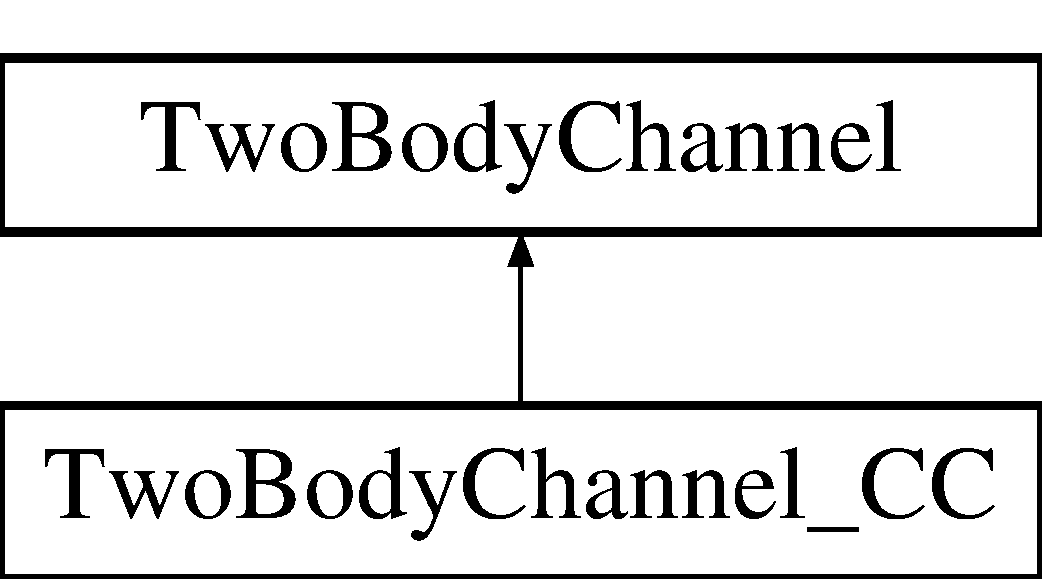
\includegraphics[height=2.000000cm]{classTwoBodyChannel}
\end{center}
\end{figure}
\subsection*{Public Member Functions}
\begin{DoxyCompactItemize}
\item 
\mbox{\Hypertarget{classTwoBodyChannel_af9b4f971e24b254b1c8bee51310f02a1}\label{classTwoBodyChannel_af9b4f971e24b254b1c8bee51310f02a1}} 
{\bfseries Two\+Body\+Channel} (int j, int p, int t, \hyperlink{classModelSpace}{Model\+Space} $\ast$ms)
\item 
\mbox{\Hypertarget{classTwoBodyChannel_a77f02ae715ac81c4d9915388c35a1941}\label{classTwoBodyChannel_a77f02ae715ac81c4d9915388c35a1941}} 
{\bfseries Two\+Body\+Channel} (int N, \hyperlink{classModelSpace}{Model\+Space} $\ast$ms)
\item 
void \hyperlink{classTwoBodyChannel_abe82c6109a1de6cfe94e8bb88b84cdc2}{Initialize} (int N, \hyperlink{classModelSpace}{Model\+Space} $\ast$ms)
\item 
\mbox{\Hypertarget{classTwoBodyChannel_adaa6d12ab3ece4a669af12f5dfedb370}\label{classTwoBodyChannel_adaa6d12ab3ece4a669af12f5dfedb370}} 
int \hyperlink{classTwoBodyChannel_adaa6d12ab3ece4a669af12f5dfedb370}{Get\+Number\+Kets} () const
\begin{DoxyCompactList}\small\item\em return Number\+Kets(\+Number of pq configs that participate in this channel) \end{DoxyCompactList}\item 
\mbox{\Hypertarget{classTwoBodyChannel_a5197ccb18558efb246099aa1ff3c5a14}\label{classTwoBodyChannel_a5197ccb18558efb246099aa1ff3c5a14}} 
int \hyperlink{classTwoBodyChannel_a5197ccb18558efb246099aa1ff3c5a14}{Get\+Local\+Index} (int ketindex) const
\begin{DoxyCompactList}\small\item\em modelspace ket index =$>$ local ket index \end{DoxyCompactList}\item 
\mbox{\Hypertarget{classTwoBodyChannel_a2224b31880155cce31003b793ca65d68}\label{classTwoBodyChannel_a2224b31880155cce31003b793ca65d68}} 
int {\bfseries Get\+Local\+Index} (int p, int q) const
\item 
\mbox{\Hypertarget{classTwoBodyChannel_a60a839eda4d1569f0f27da627be1bce6}\label{classTwoBodyChannel_a60a839eda4d1569f0f27da627be1bce6}} 
int \hyperlink{classTwoBodyChannel_a60a839eda4d1569f0f27da627be1bce6}{Get\+Ket\+Index} (int i) const
\begin{DoxyCompactList}\small\item\em local ket index =$>$ modelspace ket index \end{DoxyCompactList}\item 
\mbox{\Hypertarget{classTwoBodyChannel_aa6cf4eca0b9d1e82c0caf4744fc95d9e}\label{classTwoBodyChannel_aa6cf4eca0b9d1e82c0caf4744fc95d9e}} 
const \hyperlink{classKet}{Ket} \& \hyperlink{classTwoBodyChannel_aa6cf4eca0b9d1e82c0caf4744fc95d9e}{Get\+Ket} (int i) const
\begin{DoxyCompactList}\small\item\em get pointer to ket using local index \end{DoxyCompactList}\item 
\mbox{\Hypertarget{classTwoBodyChannel_ad4d43b775faff6cfb512d11dfed230c9}\label{classTwoBodyChannel_ad4d43b775faff6cfb512d11dfed230c9}} 
\hyperlink{classKet}{Ket} \& {\bfseries Get\+Ket} (int i)
\item 
\mbox{\Hypertarget{classTwoBodyChannel_a1e132833f7ca846b87f724dd0dfabfe2}\label{classTwoBodyChannel_a1e132833f7ca846b87f724dd0dfabfe2}} 
arma\+::uvec \hyperlink{classTwoBodyChannel_a1e132833f7ca846b87f724dd0dfabfe2}{Get\+Ket\+Index\+From\+List} (std\+::vector$<$ index\+\_\+t $>$ \&vec\+\_\+in)
\begin{DoxyCompactList}\small\item\em get \hyperlink{classKet}{Ket} index from List ? \end{DoxyCompactList}\item 
\mbox{\Hypertarget{classTwoBodyChannel_ab62d6440a9106dc9c93e0a74ac69bb1a}\label{classTwoBodyChannel_ab62d6440a9106dc9c93e0a74ac69bb1a}} 
const arma\+::uvec \& \hyperlink{classTwoBodyChannel_ab62d6440a9106dc9c93e0a74ac69bb1a}{Get\+Ket\+Index\+\_\+pp} () const
\begin{DoxyCompactList}\small\item\em get \hyperlink{classKet}{Ket} index of pp channel ? \end{DoxyCompactList}\item 
\mbox{\Hypertarget{classTwoBodyChannel_aadaffd935e935e7eeac860cce28e7db5}\label{classTwoBodyChannel_aadaffd935e935e7eeac860cce28e7db5}} 
const arma\+::uvec \& \hyperlink{classTwoBodyChannel_aadaffd935e935e7eeac860cce28e7db5}{Get\+Ket\+Index\+\_\+hh} () const
\begin{DoxyCompactList}\small\item\em get \hyperlink{classKet}{Ket} index of hh channel ? \end{DoxyCompactList}\item 
\mbox{\Hypertarget{classTwoBodyChannel_a49c55ec79a3e58a8812196e43c5891a2}\label{classTwoBodyChannel_a49c55ec79a3e58a8812196e43c5891a2}} 
const arma\+::uvec \& \hyperlink{classTwoBodyChannel_a49c55ec79a3e58a8812196e43c5891a2}{Get\+Ket\+Index\+\_\+ph} () const
\begin{DoxyCompactList}\small\item\em get \hyperlink{classKet}{Ket} index of ph channel ? \end{DoxyCompactList}\item 
\mbox{\Hypertarget{classTwoBodyChannel_ac976c6b427b6f958d1e3fa1bb0da37c4}\label{classTwoBodyChannel_ac976c6b427b6f958d1e3fa1bb0da37c4}} 
const arma\+::uvec \& \hyperlink{classTwoBodyChannel_ac976c6b427b6f958d1e3fa1bb0da37c4}{Get\+Ket\+Index\+\_\+cc} () const
\begin{DoxyCompactList}\small\item\em get \hyperlink{classKet}{Ket} index of cc channel ? \end{DoxyCompactList}\item 
\mbox{\Hypertarget{classTwoBodyChannel_a0269b5d5d31b4895031573eec92f6139}\label{classTwoBodyChannel_a0269b5d5d31b4895031573eec92f6139}} 
const arma\+::uvec \& {\bfseries Get\+Ket\+Index\+\_\+vc} () const
\item 
\mbox{\Hypertarget{classTwoBodyChannel_a910622ad4d7f85363a75bed9953586f0}\label{classTwoBodyChannel_a910622ad4d7f85363a75bed9953586f0}} 
const arma\+::uvec \& {\bfseries Get\+Ket\+Index\+\_\+qc} () const
\item 
\mbox{\Hypertarget{classTwoBodyChannel_a432bc92f03756cbb5b2c933ac7267380}\label{classTwoBodyChannel_a432bc92f03756cbb5b2c933ac7267380}} 
const arma\+::uvec \& {\bfseries Get\+Ket\+Index\+\_\+vv} () const
\item 
\mbox{\Hypertarget{classTwoBodyChannel_a2452be9ce3a7a5f78087c988fde2a387}\label{classTwoBodyChannel_a2452be9ce3a7a5f78087c988fde2a387}} 
const arma\+::uvec \& {\bfseries Get\+Ket\+Index\+\_\+qv} () const
\item 
\mbox{\Hypertarget{classTwoBodyChannel_aee32362443658da1f1d4b42687d6aaf2}\label{classTwoBodyChannel_aee32362443658da1f1d4b42687d6aaf2}} 
const arma\+::uvec \& {\bfseries Get\+Ket\+Index\+\_\+qq} () const
\item 
\mbox{\Hypertarget{classTwoBodyChannel_aa02ee6c87c6499a93233d58dc6553b48}\label{classTwoBodyChannel_aa02ee6c87c6499a93233d58dc6553b48}} 
virtual bool \hyperlink{classTwoBodyChannel_aa02ee6c87c6499a93233d58dc6553b48}{Check\+Channel\+\_\+ket} (\hyperlink{classOrbit}{Orbit} $\ast$op, \hyperlink{classOrbit}{Orbit} $\ast$oq) const
\begin{DoxyCompactList}\small\item\em check if $\vert$pq$>$ participates in this channel \end{DoxyCompactList}\item 
\mbox{\Hypertarget{classTwoBodyChannel_aee0885f4928d4b834d91120412e684d8}\label{classTwoBodyChannel_aee0885f4928d4b834d91120412e684d8}} 
bool {\bfseries Check\+Channel\+\_\+ket} (\hyperlink{classKet}{Ket} \&ket) const
\end{DoxyCompactItemize}
\subsection*{Public Attributes}
\begin{DoxyCompactItemize}
\item 
\mbox{\Hypertarget{classTwoBodyChannel_af9976c47e94db87fec18e1a546b9617f}\label{classTwoBodyChannel_af9976c47e94db87fec18e1a546b9617f}} 
int \hyperlink{classTwoBodyChannel_af9976c47e94db87fec18e1a546b9617f}{J}
\begin{DoxyCompactList}\small\item\em total angular momentum of channel \end{DoxyCompactList}\item 
\mbox{\Hypertarget{classTwoBodyChannel_a685363a37686469073bd1cef68af7d5c}\label{classTwoBodyChannel_a685363a37686469073bd1cef68af7d5c}} 
int \hyperlink{classTwoBodyChannel_a685363a37686469073bd1cef68af7d5c}{parity}
\begin{DoxyCompactList}\small\item\em parity of channel \end{DoxyCompactList}\item 
\mbox{\Hypertarget{classTwoBodyChannel_a3f40dbd98bca44d04d1f5e016d4a3bbc}\label{classTwoBodyChannel_a3f40dbd98bca44d04d1f5e016d4a3bbc}} 
int \hyperlink{classTwoBodyChannel_a3f40dbd98bca44d04d1f5e016d4a3bbc}{Tz}
\begin{DoxyCompactList}\small\item\em isospin Tz of channel \end{DoxyCompactList}\item 
\mbox{\Hypertarget{classTwoBodyChannel_ac088eba6c0d526f966a7f0544e512f72}\label{classTwoBodyChannel_ac088eba6c0d526f966a7f0544e512f72}} 
arma\+::uvec {\bfseries Ket\+Index\+\_\+pp}
\item 
\mbox{\Hypertarget{classTwoBodyChannel_acd538bd5dca3539c405fbb83277e131d}\label{classTwoBodyChannel_acd538bd5dca3539c405fbb83277e131d}} 
arma\+::uvec {\bfseries Ket\+Index\+\_\+hh}
\item 
\mbox{\Hypertarget{classTwoBodyChannel_a0379c61ac67f65a6bb167e9daf2c12fe}\label{classTwoBodyChannel_a0379c61ac67f65a6bb167e9daf2c12fe}} 
arma\+::uvec {\bfseries Ket\+Index\+\_\+ph}
\item 
\mbox{\Hypertarget{classTwoBodyChannel_ae26698f416e5b59d2a9ce1d8dbeb9454}\label{classTwoBodyChannel_ae26698f416e5b59d2a9ce1d8dbeb9454}} 
arma\+::uvec {\bfseries Ket\+Index\+\_\+cc}
\item 
\mbox{\Hypertarget{classTwoBodyChannel_a762dcd5771433d50dcfdeffa70f29c78}\label{classTwoBodyChannel_a762dcd5771433d50dcfdeffa70f29c78}} 
arma\+::uvec {\bfseries Ket\+Index\+\_\+vc}
\item 
\mbox{\Hypertarget{classTwoBodyChannel_aea3d9206d21bcc360bac06ee4d344b8d}\label{classTwoBodyChannel_aea3d9206d21bcc360bac06ee4d344b8d}} 
arma\+::uvec {\bfseries Ket\+Index\+\_\+qc}
\item 
\mbox{\Hypertarget{classTwoBodyChannel_a9233dd7b2b0dcaddf9790fd1583a411b}\label{classTwoBodyChannel_a9233dd7b2b0dcaddf9790fd1583a411b}} 
arma\+::uvec {\bfseries Ket\+Index\+\_\+vv}
\item 
\mbox{\Hypertarget{classTwoBodyChannel_a755fa9513101476da3186df726fbd822}\label{classTwoBodyChannel_a755fa9513101476da3186df726fbd822}} 
arma\+::uvec {\bfseries Ket\+Index\+\_\+qv}
\item 
\mbox{\Hypertarget{classTwoBodyChannel_a85704e33df96cc58026f2f96f44ca055}\label{classTwoBodyChannel_a85704e33df96cc58026f2f96f44ca055}} 
arma\+::uvec {\bfseries Ket\+Index\+\_\+qq}
\item 
\mbox{\Hypertarget{classTwoBodyChannel_ac0063833a374d8642cd6b4d8db7be1e2}\label{classTwoBodyChannel_ac0063833a374d8642cd6b4d8db7be1e2}} 
arma\+::vec {\bfseries Ket\+\_\+occ\+\_\+hh}
\item 
\mbox{\Hypertarget{classTwoBodyChannel_a74dc7bbce6fd62461c08be4ddb224de3}\label{classTwoBodyChannel_a74dc7bbce6fd62461c08be4ddb224de3}} 
arma\+::vec {\bfseries Ket\+\_\+unocc\+\_\+hh}
\item 
\mbox{\Hypertarget{classTwoBodyChannel_ad61411aa8b1e79b924a238c69fd9b574}\label{classTwoBodyChannel_ad61411aa8b1e79b924a238c69fd9b574}} 
arma\+::vec {\bfseries Ket\+\_\+occ\+\_\+ph}
\item 
\mbox{\Hypertarget{classTwoBodyChannel_af12dd5e981795a79aaa58e05a1012628}\label{classTwoBodyChannel_af12dd5e981795a79aaa58e05a1012628}} 
arma\+::vec {\bfseries Ket\+\_\+unocc\+\_\+ph}
\item 
\mbox{\Hypertarget{classTwoBodyChannel_a8fbda0f207db13abc96f7d6bb577c715}\label{classTwoBodyChannel_a8fbda0f207db13abc96f7d6bb577c715}} 
\hyperlink{classModelSpace}{Model\+Space} $\ast$ {\bfseries modelspace}
\item 
\mbox{\Hypertarget{classTwoBodyChannel_a7c74165bacde3f9e8fa2b6448ff48622}\label{classTwoBodyChannel_a7c74165bacde3f9e8fa2b6448ff48622}} 
int \hyperlink{classTwoBodyChannel_a7c74165bacde3f9e8fa2b6448ff48622}{Number\+Kets}
\begin{DoxyCompactList}\small\item\em Number of pq configs that participate in this channel. \end{DoxyCompactList}\item 
\mbox{\Hypertarget{classTwoBodyChannel_a55bbd64549b0c39c019eb28f6a8809ac}\label{classTwoBodyChannel_a55bbd64549b0c39c019eb28f6a8809ac}} 
std\+::vector$<$ int $>$ \hyperlink{classTwoBodyChannel_a55bbd64549b0c39c019eb28f6a8809ac}{Ket\+List}
\begin{DoxyCompactList}\small\item\em eg \mbox{[}2, 4, 7, ...\mbox{]} Used for looping over all the kets in the channel \end{DoxyCompactList}\item 
\mbox{\Hypertarget{classTwoBodyChannel_a5d353c3236f6b6067d51b9213be5e127}\label{classTwoBodyChannel_a5d353c3236f6b6067d51b9213be5e127}} 
std\+::vector$<$ int $>$ \hyperlink{classTwoBodyChannel_a5d353c3236f6b6067d51b9213be5e127}{Ket\+Map}
\begin{DoxyCompactList}\small\item\em eg \mbox{[} -\/1, -\/1, 0, -\/1, 1, -\/1, -\/1, 2 ...\mbox{]} Used for asking what is the local index of this ket. -\/1 means the ket doesn\textquotesingle{}t participate in this channel \end{DoxyCompactList}\end{DoxyCompactItemize}


\subsection{Detailed Description}
Two-\/body channel is a collection of Kets having same J,P,T in the model space

channel has Kets \{ $\vert$pq$>$ \} which can have same J,P,T. p and q can be particle/hole and core/valence/q 

\subsection{Member Function Documentation}
\mbox{\Hypertarget{classTwoBodyChannel_abe82c6109a1de6cfe94e8bb88b84cdc2}\label{classTwoBodyChannel_abe82c6109a1de6cfe94e8bb88b84cdc2}} 
\index{Two\+Body\+Channel@{Two\+Body\+Channel}!Initialize@{Initialize}}
\index{Initialize@{Initialize}!Two\+Body\+Channel@{Two\+Body\+Channel}}
\subsubsection{\texorpdfstring{Initialize()}{Initialize()}}
{\footnotesize\ttfamily void Two\+Body\+Channel\+::\+Initialize (\begin{DoxyParamCaption}\item[{int}]{N,  }\item[{\hyperlink{classModelSpace}{Model\+Space} $\ast$}]{ms }\end{DoxyParamCaption})}

construct two-\/body channels from model space

J, parity, Tz are infered from model space as

J = N\%(tbjmax+1);

parity = (N/(tbjmax+1))\%2;

Tz = (N/(2$\ast$(tbjmax+1))-\/1);

collect kets from model space for two-\/body channel \{ $\vert$pq$>$\+\_\+\{J\+PT\} \}


\begin{DoxyEnumerate}
\item J = N\%(tbjmax+1) \# it is not clear how N is defined..
\item parity = (N/(tbjmax+1))\%2;
\item Tz = (N/(2$\ast$(tbjmax+1))-\/1)
\item make Ket\+Map from model space Kets by Check\+Channel\+\_\+ket(ket)
\item Get Ket\+Index\+\_\+pp in this channel from modelspace Ket\+Index\+\_\+pp. other index of \+\_\+hh,\+\_\+ph,\+\_\+cc ..in a similar way.
\item Get Ket\+\_\+occ\+\_\+hh and Ket\+\_\+unocc\+\_\+hh in this channel from model space. Ket\+\_\+occ\+\_\+ph Ket\+\_\+unocc\+\_\+ph in a similar way 
\end{DoxyEnumerate}

The documentation for this class was generated from the following files\+:\begin{DoxyCompactItemize}
\item 
Model\+Space.\+hh\item 
Model\+Space.\+cc\end{DoxyCompactItemize}

\hypertarget{classTwoBodyChannel__CC}{}\section{Two\+Body\+Channel\+\_\+\+CC Class Reference}
\label{classTwoBodyChannel__CC}\index{Two\+Body\+Channel\+\_\+\+CC@{Two\+Body\+Channel\+\_\+\+CC}}


cross-\/coupled two-\/body channel (allows $<$pp$\vert$$\vert$nn$>$ but no $<$pp$\vert$$\vert$pn$>$ i.\+e. same $\vert$\+T\+\_\+z$\vert$)  




{\ttfamily \#include $<$Model\+Space.\+hh$>$}

Inheritance diagram for Two\+Body\+Channel\+\_\+\+CC\+:\begin{figure}[H]
\begin{center}
\leavevmode
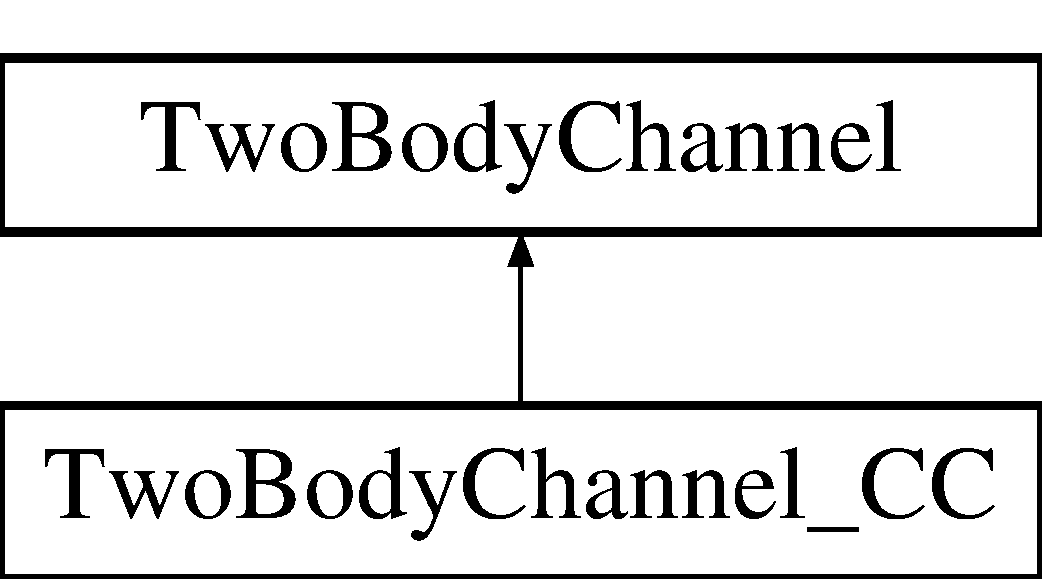
\includegraphics[height=2.000000cm]{classTwoBodyChannel__CC}
\end{center}
\end{figure}
\subsection*{Public Member Functions}
\begin{DoxyCompactItemize}
\item 
\mbox{\Hypertarget{classTwoBodyChannel__CC_add1c09d721a004cf2280111746ade74f}\label{classTwoBodyChannel__CC_add1c09d721a004cf2280111746ade74f}} 
{\bfseries Two\+Body\+Channel\+\_\+\+CC} (int j, int p, int t, \hyperlink{classModelSpace}{Model\+Space} $\ast$ms)
\item 
\mbox{\Hypertarget{classTwoBodyChannel__CC_ac10877d81204c16e095417d5eb7daa95}\label{classTwoBodyChannel__CC_ac10877d81204c16e095417d5eb7daa95}} 
{\bfseries Two\+Body\+Channel\+\_\+\+CC} (int N, \hyperlink{classModelSpace}{Model\+Space} $\ast$ms)
\item 
bool \hyperlink{classTwoBodyChannel__CC_a9a73ccfd9ba18bbc840547669254ef79}{Check\+Channel\+\_\+ket} (\hyperlink{classOrbit}{Orbit} $\ast$op, \hyperlink{classOrbit}{Orbit} $\ast$oq) const
\begin{DoxyCompactList}\small\item\em check if $\vert$pq$>$ participates in this channel \end{DoxyCompactList}\end{DoxyCompactItemize}
\subsection*{Additional Inherited Members}


\subsection{Detailed Description}
cross-\/coupled two-\/body channel (allows $<$pp$\vert$$\vert$nn$>$ but no $<$pp$\vert$$\vert$pn$>$ i.\+e. same $\vert$\+T\+\_\+z$\vert$) 

\subsection{Member Function Documentation}
\mbox{\Hypertarget{classTwoBodyChannel__CC_a9a73ccfd9ba18bbc840547669254ef79}\label{classTwoBodyChannel__CC_a9a73ccfd9ba18bbc840547669254ef79}} 
\index{Two\+Body\+Channel\+\_\+\+CC@{Two\+Body\+Channel\+\_\+\+CC}!Check\+Channel\+\_\+ket@{Check\+Channel\+\_\+ket}}
\index{Check\+Channel\+\_\+ket@{Check\+Channel\+\_\+ket}!Two\+Body\+Channel\+\_\+\+CC@{Two\+Body\+Channel\+\_\+\+CC}}
\subsubsection{\texorpdfstring{Check\+Channel\+\_\+ket()}{CheckChannel\_ket()}}
{\footnotesize\ttfamily bool Two\+Body\+Channel\+\_\+\+C\+C\+::\+Check\+Channel\+\_\+ket (\begin{DoxyParamCaption}\item[{\hyperlink{classOrbit}{Orbit} $\ast$}]{op,  }\item[{\hyperlink{classOrbit}{Orbit} $\ast$}]{oq }\end{DoxyParamCaption}) const\hspace{0.3cm}{\ttfamily [virtual]}}



check if $\vert$pq$>$ participates in this channel 

Check if orbits pq participate in this cross-\/coupled two-\/body channel

Difference from regular channels\+: no Pauli rule, $<$pp$\vert$$\vert$nn$>$ is allowed. But $\vert$\+Tz$\vert$ is still conserved, i.\+e. $<$pp$\vert$$\vert$pn$>$ is not allowed. So we use $\vert$\+Tz$\vert$ rather than Tz, and don\textquotesingle{}t use Tz=-\/1. 

Reimplemented from \hyperlink{classTwoBodyChannel_aa02ee6c87c6499a93233d58dc6553b48}{Two\+Body\+Channel}.



The documentation for this class was generated from the following files\+:\begin{DoxyCompactItemize}
\item 
Model\+Space.\+hh\item 
Model\+Space.\+cc\end{DoxyCompactItemize}

\hypertarget{classTwoBodyME}{}\section{Two\+Body\+ME Class Reference}
\label{classTwoBodyME}\index{Two\+Body\+ME@{Two\+Body\+ME}}


{\ttfamily \#include $<$Two\+Body\+M\+E.\+hh$>$}

\subsection*{Public Member Functions}
\begin{DoxyCompactItemize}
\item 
\mbox{\Hypertarget{classTwoBodyME_ab83ecb946db481f645f203e76ea3db52}\label{classTwoBodyME_ab83ecb946db481f645f203e76ea3db52}} 
{\bfseries Two\+Body\+ME} (\hyperlink{classModelSpace}{Model\+Space} $\ast$)
\item 
\mbox{\Hypertarget{classTwoBodyME_a059914b2a21bac504d566540b611fe37}\label{classTwoBodyME_a059914b2a21bac504d566540b611fe37}} 
{\bfseries Two\+Body\+ME} (Two\+Body\+M\+E\+\_\+ph \&)
\item 
\mbox{\Hypertarget{classTwoBodyME_a493598d48d18fdd38c056ebf89376dc9}\label{classTwoBodyME_a493598d48d18fdd38c056ebf89376dc9}} 
{\bfseries Two\+Body\+ME} (\hyperlink{classModelSpace}{Model\+Space} $\ast$ms, int rankJ, int rankT, int parity)
\item 
\mbox{\Hypertarget{classTwoBodyME_a0e511eefd39cdf5112d86bc4a0a0414a}\label{classTwoBodyME_a0e511eefd39cdf5112d86bc4a0a0414a}} 
\hyperlink{classTwoBodyME}{Two\+Body\+ME} \& {\bfseries operator$\ast$=} (const double)
\item 
\mbox{\Hypertarget{classTwoBodyME_acad0fc7cee36df621b8c4be14b3d5505}\label{classTwoBodyME_acad0fc7cee36df621b8c4be14b3d5505}} 
\hyperlink{classTwoBodyME}{Two\+Body\+ME} \& {\bfseries operator+=} (const \hyperlink{classTwoBodyME}{Two\+Body\+ME} \&)
\item 
\mbox{\Hypertarget{classTwoBodyME_a6922afa4634c683b899dd99a3d49f913}\label{classTwoBodyME_a6922afa4634c683b899dd99a3d49f913}} 
\hyperlink{classTwoBodyME}{Two\+Body\+ME} \& {\bfseries operator-\/=} (const \hyperlink{classTwoBodyME}{Two\+Body\+ME} \&)
\item 
\mbox{\Hypertarget{classTwoBodyME_a27ad6f262c2371d2f8eab3747af594ad}\label{classTwoBodyME_a27ad6f262c2371d2f8eab3747af594ad}} 
void {\bfseries Allocate} ()
\item 
\mbox{\Hypertarget{classTwoBodyME_a822e0bdd66bc67532f6e244eb496ff20}\label{classTwoBodyME_a822e0bdd66bc67532f6e244eb496ff20}} 
bool {\bfseries Is\+Hermitian} ()
\item 
\mbox{\Hypertarget{classTwoBodyME_aee424b280d0cdfb44fecbf5b0ec5c23d}\label{classTwoBodyME_aee424b280d0cdfb44fecbf5b0ec5c23d}} 
bool {\bfseries Is\+Anti\+Hermitian} ()
\item 
\mbox{\Hypertarget{classTwoBodyME_af3a2034735ce16504ca51459e29932e7}\label{classTwoBodyME_af3a2034735ce16504ca51459e29932e7}} 
bool {\bfseries Is\+Non\+Hermitian} ()
\item 
\mbox{\Hypertarget{classTwoBodyME_ae3d48007a67b3ab8e97232fd84812dce}\label{classTwoBodyME_ae3d48007a67b3ab8e97232fd84812dce}} 
void {\bfseries Set\+Hermitian} ()
\item 
\mbox{\Hypertarget{classTwoBodyME_ab782a80a918095a69189a0f9d2e43e44}\label{classTwoBodyME_ab782a80a918095a69189a0f9d2e43e44}} 
void {\bfseries Set\+Anti\+Hermitian} ()
\item 
\mbox{\Hypertarget{classTwoBodyME_af71f00cd1035917147f048156ee20072}\label{classTwoBodyME_af71f00cd1035917147f048156ee20072}} 
void {\bfseries Set\+Non\+Hermitian} ()
\item 
\mbox{\Hypertarget{classTwoBodyME_a76241fa6336d763b47f3619e5c4b2963}\label{classTwoBodyME_a76241fa6336d763b47f3619e5c4b2963}} 
arma\+::mat \& {\bfseries Get\+Matrix} (int chbra, int chket)
\item 
\mbox{\Hypertarget{classTwoBodyME_abba656ff6b5773a16424b71fe6f3c73f}\label{classTwoBodyME_abba656ff6b5773a16424b71fe6f3c73f}} 
arma\+::mat \& {\bfseries Get\+Matrix} (int ch)
\item 
\mbox{\Hypertarget{classTwoBodyME_a676e0c9ef53e7ad937713b0bb518f94b}\label{classTwoBodyME_a676e0c9ef53e7ad937713b0bb518f94b}} 
arma\+::mat \& {\bfseries Get\+Matrix} (std\+::array$<$ int, 2 $>$ a)
\item 
\mbox{\Hypertarget{classTwoBodyME_aa2ed0dcf17e0eb7dd38a0c7bf2df8562}\label{classTwoBodyME_aa2ed0dcf17e0eb7dd38a0c7bf2df8562}} 
const arma\+::mat \& {\bfseries Get\+Matrix} (int chbra, int chket) const
\item 
\mbox{\Hypertarget{classTwoBodyME_a209a1bcc3286c165b426e33845b1455d}\label{classTwoBodyME_a209a1bcc3286c165b426e33845b1455d}} 
const arma\+::mat \& {\bfseries Get\+Matrix} (int ch) const
\item 
\mbox{\Hypertarget{classTwoBodyME_a86c81a876ec642f8a28750df4d0c1907}\label{classTwoBodyME_a86c81a876ec642f8a28750df4d0c1907}} 
double \hyperlink{classTwoBodyME_a86c81a876ec642f8a28750df4d0c1907}{Get\+T\+B\+ME} (int ch\+\_\+bra, int ch\+\_\+ket, int a, int b, int c, int d) const
\begin{DoxyCompactList}\small\item\em This returns the matrix element times a factor $ \sqrt{(1+\delta_{ij})(1+\delta_{kl})} $. \end{DoxyCompactList}\item 
\mbox{\Hypertarget{classTwoBodyME_a26ca6f74a4815c5b23c82fe2c29f8f36}\label{classTwoBodyME_a26ca6f74a4815c5b23c82fe2c29f8f36}} 
double \hyperlink{classTwoBodyME_a26ca6f74a4815c5b23c82fe2c29f8f36}{Get\+T\+B\+M\+E\+\_\+norm} (int ch\+\_\+bra, int ch\+\_\+ket, int a, int b, int c, int d) const
\begin{DoxyCompactList}\small\item\em This returns the normalized matrix element. \end{DoxyCompactList}\item 
\mbox{\Hypertarget{classTwoBodyME_a361aa001f5e09b6a906bbd0504582e2b}\label{classTwoBodyME_a361aa001f5e09b6a906bbd0504582e2b}} 
void {\bfseries Set\+T\+B\+ME} (int ch\+\_\+bra, int ch\+\_\+ket, int a, int b, int c, int d, double tbme)
\item 
\mbox{\Hypertarget{classTwoBodyME_af5c7ce4cf4638b7946db6aa01b502455}\label{classTwoBodyME_af5c7ce4cf4638b7946db6aa01b502455}} 
void {\bfseries Add\+To\+T\+B\+ME} (int ch\+\_\+bra, int ch\+\_\+ket, int a, int b, int c, int d, double tbme)
\item 
\mbox{\Hypertarget{classTwoBodyME_a5e6112c43feadffc5b5eb0c01aaa0f7c}\label{classTwoBodyME_a5e6112c43feadffc5b5eb0c01aaa0f7c}} 
double {\bfseries Get\+T\+B\+ME} (int ch\+\_\+bra, int ch\+\_\+ket, \hyperlink{classKet}{Ket} \&bra, \hyperlink{classKet}{Ket} \&ket) const
\item 
\mbox{\Hypertarget{classTwoBodyME_a3c217bf0da82dd9a4bfbe364852af672}\label{classTwoBodyME_a3c217bf0da82dd9a4bfbe364852af672}} 
void {\bfseries Set\+T\+B\+ME} (int ch\+\_\+bra, int ch\+\_\+ket, \hyperlink{classKet}{Ket} \&bra, \hyperlink{classKet}{Ket} \&ket, double tbme)
\item 
\mbox{\Hypertarget{classTwoBodyME_a314e2a6279e88c00c8ae5a2f12a73a59}\label{classTwoBodyME_a314e2a6279e88c00c8ae5a2f12a73a59}} 
void {\bfseries Add\+To\+T\+B\+ME} (int ch\+\_\+bra, int ch\+\_\+ket, \hyperlink{classKet}{Ket} \&bra, \hyperlink{classKet}{Ket} \&ket, double tbme)
\item 
\mbox{\Hypertarget{classTwoBodyME_a1fd7f49611b96d44705684b63480e5ff}\label{classTwoBodyME_a1fd7f49611b96d44705684b63480e5ff}} 
double {\bfseries Get\+T\+B\+M\+E\+\_\+norm} (int ch\+\_\+bra, int ch\+\_\+ket, int ibra, int iket) const
\item 
\mbox{\Hypertarget{classTwoBodyME_a70964978f2900035b751b152f69dece1}\label{classTwoBodyME_a70964978f2900035b751b152f69dece1}} 
void {\bfseries Set\+T\+B\+ME} (int ch\+\_\+bra, int ch\+\_\+ket, int ibra, int iket, double tbme)
\item 
\mbox{\Hypertarget{classTwoBodyME_a6191d7b60382fe36cf323a63386fb032}\label{classTwoBodyME_a6191d7b60382fe36cf323a63386fb032}} 
void {\bfseries Add\+To\+T\+B\+ME} (int ch\+\_\+bra, int ch\+\_\+ket, int ibra, int iket, double tbme)
\item 
\mbox{\Hypertarget{classTwoBodyME_a2c073e3f4daed440609d8f7a45a8cf53}\label{classTwoBodyME_a2c073e3f4daed440609d8f7a45a8cf53}} 
double {\bfseries Get\+T\+B\+ME} (int j\+\_\+bra, int p\+\_\+bra, int t\+\_\+bra, int j\+\_\+ket, int p\+\_\+ket, int t\+\_\+ket, \hyperlink{classKet}{Ket} \&bra, \hyperlink{classKet}{Ket} \&ket) const
\item 
\mbox{\Hypertarget{classTwoBodyME_af3441f4f28102dd66c31ad5d67bba5c4}\label{classTwoBodyME_af3441f4f28102dd66c31ad5d67bba5c4}} 
void {\bfseries Set\+T\+B\+ME} (int j\+\_\+bra, int p\+\_\+bra, int t\+\_\+bra, int j\+\_\+ket, int p\+\_\+ket, int t\+\_\+ket, \hyperlink{classKet}{Ket} \&bra, \hyperlink{classKet}{Ket} \&ket, double tbme)
\item 
\mbox{\Hypertarget{classTwoBodyME_af3d13a2434e9614de1a40a78c0c16ba1}\label{classTwoBodyME_af3d13a2434e9614de1a40a78c0c16ba1}} 
void {\bfseries Add\+To\+T\+B\+ME} (int j\+\_\+bra, int p\+\_\+bra, int t\+\_\+bra, int j\+\_\+ket, int p\+\_\+ket, int t\+\_\+ket, \hyperlink{classKet}{Ket} \&bra, \hyperlink{classKet}{Ket} \&ket, double tbme)
\item 
\mbox{\Hypertarget{classTwoBodyME_aac838c8a4fbff88efd7c7ba70cf80873}\label{classTwoBodyME_aac838c8a4fbff88efd7c7ba70cf80873}} 
double {\bfseries Get\+T\+B\+ME} (int j\+\_\+bra, int p\+\_\+bra, int t\+\_\+bra, int j\+\_\+ket, int p\+\_\+ket, int t\+\_\+ket, int a, int b, int c, int d) const
\item 
\mbox{\Hypertarget{classTwoBodyME_abea5301c27dd939a7e5269405aaf9291}\label{classTwoBodyME_abea5301c27dd939a7e5269405aaf9291}} 
void {\bfseries Set\+T\+B\+ME} (int j\+\_\+bra, int p\+\_\+bra, int t\+\_\+bra, int j\+\_\+ket, int p\+\_\+ket, int t\+\_\+ket, int a, int b, int c, int d, double tbme)
\item 
\mbox{\Hypertarget{classTwoBodyME_ae29ace6699855265f35a5c5d8b4a4baf}\label{classTwoBodyME_ae29ace6699855265f35a5c5d8b4a4baf}} 
void {\bfseries Add\+To\+T\+B\+ME} (int j\+\_\+bra, int p\+\_\+bra, int t\+\_\+bra, int j\+\_\+ket, int p\+\_\+ket, int t\+\_\+ket, int a, int b, int c, int d, double tbme)
\item 
\mbox{\Hypertarget{classTwoBodyME_a385455012cf6f22fb94a218c70ce25e8}\label{classTwoBodyME_a385455012cf6f22fb94a218c70ce25e8}} 
double {\bfseries Get\+T\+B\+M\+E\+\_\+J} (int j\+\_\+bra, int j\+\_\+ket, int a, int b, int c, int d) const
\item 
\mbox{\Hypertarget{classTwoBodyME_a5f3f5cff3f7908b53d280a3e3c6d335c}\label{classTwoBodyME_a5f3f5cff3f7908b53d280a3e3c6d335c}} 
void {\bfseries Set\+T\+B\+M\+E\+\_\+J} (int j\+\_\+bra, int j\+\_\+ket, int a, int b, int c, int d, double tbme)
\item 
\mbox{\Hypertarget{classTwoBodyME_a99e7650830fdc19a7d7fef5d0be8d7f2}\label{classTwoBodyME_a99e7650830fdc19a7d7fef5d0be8d7f2}} 
void {\bfseries Add\+To\+T\+B\+M\+E\+\_\+J} (int j\+\_\+bra, int j\+\_\+ket, int a, int b, int c, int d, double tbme)
\item 
\mbox{\Hypertarget{classTwoBodyME_ab5df6a8eca64b0e88ebcff3b1a1d04e3}\label{classTwoBodyME_ab5df6a8eca64b0e88ebcff3b1a1d04e3}} 
double {\bfseries Get\+T\+B\+M\+E\+\_\+\+J\+\_\+norm} (int j\+\_\+bra, int j\+\_\+ket, int a, int b, int c, int d) const
\item 
\mbox{\Hypertarget{classTwoBodyME_a04aa5b2c179869ec42d8b7b554db58bd}\label{classTwoBodyME_a04aa5b2c179869ec42d8b7b554db58bd}} 
double {\bfseries Get\+T\+B\+ME} (int ch, int a, int b, int c, int d) const
\item 
\mbox{\Hypertarget{classTwoBodyME_a722a433a9f256ea269e6c827f185926b}\label{classTwoBodyME_a722a433a9f256ea269e6c827f185926b}} 
double {\bfseries Get\+T\+B\+M\+E\+\_\+norm} (int ch, int a, int b, int c, int d) const
\item 
\mbox{\Hypertarget{classTwoBodyME_a255f61e91a2cee85cd34714bc5132221}\label{classTwoBodyME_a255f61e91a2cee85cd34714bc5132221}} 
void {\bfseries Set\+T\+B\+ME} (int ch, int a, int b, int c, int d, double tbme)
\item 
\mbox{\Hypertarget{classTwoBodyME_a202536f8f9cb8c74f1976d9bbafdaaf8}\label{classTwoBodyME_a202536f8f9cb8c74f1976d9bbafdaaf8}} 
void {\bfseries Add\+To\+T\+B\+ME} (int ch, int a, int b, int c, int d, double tbme)
\item 
\mbox{\Hypertarget{classTwoBodyME_aae40b7e6005d6afe4ed69a7ff8a201cb}\label{classTwoBodyME_aae40b7e6005d6afe4ed69a7ff8a201cb}} 
double {\bfseries Get\+T\+B\+ME} (int ch, \hyperlink{classKet}{Ket} \&bra, \hyperlink{classKet}{Ket} \&ket) const
\item 
\mbox{\Hypertarget{classTwoBodyME_a57db036e0c5c13219339d9e6b775a3c0}\label{classTwoBodyME_a57db036e0c5c13219339d9e6b775a3c0}} 
double {\bfseries Get\+T\+B\+M\+E\+\_\+norm} (int ch, \hyperlink{classKet}{Ket} \&bra, \hyperlink{classKet}{Ket} \&ket) const
\item 
\mbox{\Hypertarget{classTwoBodyME_a8b42151c12ae112e507e1ab9b1053427}\label{classTwoBodyME_a8b42151c12ae112e507e1ab9b1053427}} 
void {\bfseries Set\+T\+B\+ME} (int ch, \hyperlink{classKet}{Ket} \&bra, \hyperlink{classKet}{Ket} \&ket, double tbme)
\item 
\mbox{\Hypertarget{classTwoBodyME_a0e92d946139161a62151508fd82b545f}\label{classTwoBodyME_a0e92d946139161a62151508fd82b545f}} 
void {\bfseries Add\+To\+T\+B\+ME} (int ch, \hyperlink{classKet}{Ket} \&bra, \hyperlink{classKet}{Ket} \&ket, double tbme)
\item 
\mbox{\Hypertarget{classTwoBodyME_a5a27797e50e4203c678a812b061d0d9e}\label{classTwoBodyME_a5a27797e50e4203c678a812b061d0d9e}} 
double {\bfseries Get\+T\+B\+M\+E\+\_\+norm} (int ch, int ibra, int iket) const
\item 
\mbox{\Hypertarget{classTwoBodyME_a194371fee0b854e0c7342943a41aa28e}\label{classTwoBodyME_a194371fee0b854e0c7342943a41aa28e}} 
void {\bfseries Set\+T\+B\+ME} (int ch, int ibra, int iket, double tbme)
\item 
\mbox{\Hypertarget{classTwoBodyME_a97d624575ad1eb7704d5b46fead19b20}\label{classTwoBodyME_a97d624575ad1eb7704d5b46fead19b20}} 
void {\bfseries Add\+To\+T\+B\+ME} (int ch, int ibra, int iket, double tbme)
\item 
\mbox{\Hypertarget{classTwoBodyME_afbdedfaf6ae67aa7b151fded81113bd2}\label{classTwoBodyME_afbdedfaf6ae67aa7b151fded81113bd2}} 
double {\bfseries Get\+T\+B\+ME} (int j, int p, int t, \hyperlink{classKet}{Ket} \&bra, \hyperlink{classKet}{Ket} \&ket) const
\item 
\mbox{\Hypertarget{classTwoBodyME_a68578ba3df3f1b511d295d48071886ee}\label{classTwoBodyME_a68578ba3df3f1b511d295d48071886ee}} 
void {\bfseries Set\+T\+B\+ME} (int j, int p, int t, \hyperlink{classKet}{Ket} \&bra, \hyperlink{classKet}{Ket} \&ket, double tbme)
\item 
\mbox{\Hypertarget{classTwoBodyME_afab3a9c6c8bdca85fba816a94b326217}\label{classTwoBodyME_afab3a9c6c8bdca85fba816a94b326217}} 
void {\bfseries Add\+To\+T\+B\+ME} (int j, int p, int t, \hyperlink{classKet}{Ket} \&bra, \hyperlink{classKet}{Ket} \&ket, double tbme)
\item 
\mbox{\Hypertarget{classTwoBodyME_a39ae626faf77c3548479226897482706}\label{classTwoBodyME_a39ae626faf77c3548479226897482706}} 
double {\bfseries Get\+T\+B\+ME} (int j, int p, int t, int a, int b, int c, int d) const
\item 
\mbox{\Hypertarget{classTwoBodyME_af7a447f398390e3f536a22fcece3b677}\label{classTwoBodyME_af7a447f398390e3f536a22fcece3b677}} 
double {\bfseries Get\+T\+B\+M\+E\+\_\+norm} (int j, int p, int t, int a, int b, int c, int d) const
\item 
\mbox{\Hypertarget{classTwoBodyME_a5e7801ffab553d88ff8e2ef6e706e013}\label{classTwoBodyME_a5e7801ffab553d88ff8e2ef6e706e013}} 
void {\bfseries Set\+T\+B\+ME} (int j, int p, int t, int a, int b, int c, int d, double tbme)
\item 
\mbox{\Hypertarget{classTwoBodyME_a0c87a5d98d044af0cd9995653264b5a9}\label{classTwoBodyME_a0c87a5d98d044af0cd9995653264b5a9}} 
void {\bfseries Add\+To\+T\+B\+ME} (int j, int p, int t, int a, int b, int c, int d, double tbme)
\item 
\mbox{\Hypertarget{classTwoBodyME_aa2da878a0a9a14d9e37ebc2e8bfcfb3a}\label{classTwoBodyME_aa2da878a0a9a14d9e37ebc2e8bfcfb3a}} 
double {\bfseries Get\+T\+B\+M\+E\+\_\+J} (int j, int a, int b, int c, int d) const
\item 
\mbox{\Hypertarget{classTwoBodyME_a796ab8b1112f1acc7eb5d6b886fa9865}\label{classTwoBodyME_a796ab8b1112f1acc7eb5d6b886fa9865}} 
void {\bfseries Set\+T\+B\+M\+E\+\_\+J} (int j, int a, int b, int c, int d, double tbme)
\item 
\mbox{\Hypertarget{classTwoBodyME_ad2fed429571805bd4d8aa07a5d3903f1}\label{classTwoBodyME_ad2fed429571805bd4d8aa07a5d3903f1}} 
void {\bfseries Add\+To\+T\+B\+M\+E\+\_\+J} (int j, int a, int b, int c, int d, double tbme)
\item 
\mbox{\Hypertarget{classTwoBodyME_a2e9eb9c3f053e26e88fe8cda70ed0a21}\label{classTwoBodyME_a2e9eb9c3f053e26e88fe8cda70ed0a21}} 
double {\bfseries Get\+T\+B\+M\+E\+\_\+\+J\+\_\+norm} (int j, int a, int b, int c, int d) const
\item 
void \hyperlink{classTwoBodyME_adc76bb65d2b3bc2006a70fb2a61464c9}{Set\+\_\+pn\+\_\+\+T\+B\+M\+E\+\_\+from\+\_\+iso} (int j, int T, int tz, int a, int b, int c, int d, double tbme)
\item 
\mbox{\Hypertarget{classTwoBodyME_a98aa9dc5ab0e1d66be59e4266e4000d2}\label{classTwoBodyME_a98aa9dc5ab0e1d66be59e4266e4000d2}} 
double {\bfseries Get\+\_\+iso\+\_\+\+T\+B\+M\+E\+\_\+from\+\_\+pn} (int j, int T, int tz, int a, int b, int c, int d)
\item 
double \hyperlink{classTwoBodyME_a41e1d7a520f31b57283b7817a35bceb7}{Get\+T\+B\+M\+Emonopole} (int a, int b, int c, int d) const
\item 
\mbox{\Hypertarget{classTwoBodyME_a4ae220acdb84f7b77e96304224fda0ba}\label{classTwoBodyME_a4ae220acdb84f7b77e96304224fda0ba}} 
double {\bfseries Get\+T\+B\+M\+Emonopole\+\_\+norm} (int a, int b, int c, int d) const
\item 
\mbox{\Hypertarget{classTwoBodyME_a5d53d53d4ba757974c2ffe6ebabd4911}\label{classTwoBodyME_a5d53d53d4ba757974c2ffe6ebabd4911}} 
double {\bfseries Get\+T\+B\+M\+Emonopole} (\hyperlink{classKet}{Ket} \&bra, \hyperlink{classKet}{Ket} \&ket) const
\item 
void \hyperlink{classTwoBodyME_acd6f31eaef7652136740204ce5c4d226}{Erase} ()
\begin{DoxyCompactList}\small\item\em Take a matrix element expressed in relative/\+CM frame, and add it to the lab frame T\+B\+ME. \end{DoxyCompactList}\item 
\mbox{\Hypertarget{classTwoBodyME_a5084b43918669e7876887ed44a145f3b}\label{classTwoBodyME_a5084b43918669e7876887ed44a145f3b}} 
void {\bfseries Scale} (double)
\item 
\mbox{\Hypertarget{classTwoBodyME_a3fa4bbb2ab3359aa9d0d9035659c839b}\label{classTwoBodyME_a3fa4bbb2ab3359aa9d0d9035659c839b}} 
double {\bfseries Norm} () const
\item 
\mbox{\Hypertarget{classTwoBodyME_aefe69c49a0fd79f35b9541539b1767ce}\label{classTwoBodyME_aefe69c49a0fd79f35b9541539b1767ce}} 
void {\bfseries Symmetrize} ()
\item 
\mbox{\Hypertarget{classTwoBodyME_a30f4d86bda647d3688b1b0aaa20efb2d}\label{classTwoBodyME_a30f4d86bda647d3688b1b0aaa20efb2d}} 
void {\bfseries Anti\+Symmetrize} ()
\item 
\mbox{\Hypertarget{classTwoBodyME_a3e5d862e3471a5090d3498cf0103d07c}\label{classTwoBodyME_a3e5d862e3471a5090d3498cf0103d07c}} 
void {\bfseries Eye} ()
\item 
\mbox{\Hypertarget{classTwoBodyME_aad1e0f5311c52fa7caf07694ead3a949}\label{classTwoBodyME_aad1e0f5311c52fa7caf07694ead3a949}} 
void {\bfseries Print\+Matrix} (int chbra, int chket) const
\item 
\mbox{\Hypertarget{classTwoBodyME_a51cc0901f3bab4c288a2be006f72513a}\label{classTwoBodyME_a51cc0901f3bab4c288a2be006f72513a}} 
int {\bfseries Dimension} ()
\item 
\mbox{\Hypertarget{classTwoBodyME_ab13203f1f3d383fd241650f175cf5bb5}\label{classTwoBodyME_ab13203f1f3d383fd241650f175cf5bb5}} 
int {\bfseries size} ()
\item 
\mbox{\Hypertarget{classTwoBodyME_adb64bdb222c28be1b32467681111b1ec}\label{classTwoBodyME_adb64bdb222c28be1b32467681111b1ec}} 
void {\bfseries Write\+Binary} (std\+::ofstream \&)
\item 
\mbox{\Hypertarget{classTwoBodyME_a97fb923863bbaf7464115040e4e3cc3d}\label{classTwoBodyME_a97fb923863bbaf7464115040e4e3cc3d}} 
void {\bfseries Read\+Binary} (std\+::ifstream \&)
\end{DoxyCompactItemize}
\subsection*{Public Attributes}
\begin{DoxyCompactItemize}
\item 
\mbox{\Hypertarget{classTwoBodyME_af80319b759d9f0a1409e429def4dfbd7}\label{classTwoBodyME_af80319b759d9f0a1409e429def4dfbd7}} 
\hyperlink{classModelSpace}{Model\+Space} $\ast$ {\bfseries modelspace}
\item 
\mbox{\Hypertarget{classTwoBodyME_a3d9a200451347886bd72b94e47b30750}\label{classTwoBodyME_a3d9a200451347886bd72b94e47b30750}} 
std\+::map$<$ std\+::array$<$ int, 2 $>$, arma\+::mat $>$ {\bfseries Mat\+El}
\item 
\mbox{\Hypertarget{classTwoBodyME_aa389c365fc444a554a4e253df10f14c9}\label{classTwoBodyME_aa389c365fc444a554a4e253df10f14c9}} 
int {\bfseries n\+Channels}
\item 
\mbox{\Hypertarget{classTwoBodyME_ad29c6a4d543d73f008503312ac4184bf}\label{classTwoBodyME_ad29c6a4d543d73f008503312ac4184bf}} 
bool {\bfseries hermitian}
\item 
\mbox{\Hypertarget{classTwoBodyME_a1483d9997eee9c3b9aff840488ebb09a}\label{classTwoBodyME_a1483d9997eee9c3b9aff840488ebb09a}} 
bool {\bfseries antihermitian}
\item 
\mbox{\Hypertarget{classTwoBodyME_a2582cd10bbc17baf24dae2d8a25e78da}\label{classTwoBodyME_a2582cd10bbc17baf24dae2d8a25e78da}} 
int {\bfseries rank\+\_\+J}
\item 
\mbox{\Hypertarget{classTwoBodyME_a1f82dd6078226acd0afbe3b510b7098a}\label{classTwoBodyME_a1f82dd6078226acd0afbe3b510b7098a}} 
int {\bfseries rank\+\_\+T}
\item 
\mbox{\Hypertarget{classTwoBodyME_af4dc0e00484359f1f880e07ecc599cae}\label{classTwoBodyME_af4dc0e00484359f1f880e07ecc599cae}} 
int {\bfseries parity}
\end{DoxyCompactItemize}


\subsection{Detailed Description}
The two-\/body piece of the operator, stored in a vector of maps of of armadillo matrices. The index of the vector indicates the J-\/coupled two-\/body channel of the ket state, while the map key is the two-\/body channel of the bra state. This is done to allow for tensor operators which connect different two-\/body channels without having to store all possible combinations. In the case of a scalar operator, there is only one map key for the bra state, corresponding to that of the ket state. The normalized J-\/coupled T\+B\+ME\textquotesingle{}s are stored in the matrices. However, when the T\+B\+ME\textquotesingle{}s are accessed by \hyperlink{classTwoBodyME_a86c81a876ec642f8a28750df4d0c1907}{Get\+T\+B\+M\+E()}, they are returned as $ \tilde{\Gamma}_{ijkl} \equiv \sqrt{(1+\delta_{ij})(1+\delta_{kl})} \Gamma_{ijkl} $ because the flow equations are derived in terms of $ \tilde{\Gamma} $. For efficiency, only matrix elements with $ i\leq j $ and $ k\leq l $ are stored. When performing sums that can be cast as matrix multiplication, we have something of the form \[ \tilde{Z}_{ijkl} \sim \frac{1}{2} \sum_{ab}\tilde{X}_{ijab} \tilde{Y}_{abkl} \] which may be rewritten as a restricted sum, or matrix multiplication \[ Z_{ijkl} \sim \sum_{a\leq b} X_{ijab} Y_{abkl} = \left( X\cdot Y \right)_{ijkl} \] 

\subsection{Member Function Documentation}
\mbox{\Hypertarget{classTwoBodyME_acd6f31eaef7652136740204ce5c4d226}\label{classTwoBodyME_acd6f31eaef7652136740204ce5c4d226}} 
\index{Two\+Body\+ME@{Two\+Body\+ME}!Erase@{Erase}}
\index{Erase@{Erase}!Two\+Body\+ME@{Two\+Body\+ME}}
\subsubsection{\texorpdfstring{Erase()}{Erase()}}
{\footnotesize\ttfamily void Two\+Body\+M\+E\+::\+Erase (\begin{DoxyParamCaption}{ }\end{DoxyParamCaption})}



Take a matrix element expressed in relative/\+CM frame, and add it to the lab frame T\+B\+ME. 

For a given ket expressed in relative/\+CM coordinates, return the indices of all the lab frame kets with non-\/zero overlap, as well as the overlap \mbox{\Hypertarget{classTwoBodyME_a41e1d7a520f31b57283b7817a35bceb7}\label{classTwoBodyME_a41e1d7a520f31b57283b7817a35bceb7}} 
\index{Two\+Body\+ME@{Two\+Body\+ME}!Get\+T\+B\+M\+Emonopole@{Get\+T\+B\+M\+Emonopole}}
\index{Get\+T\+B\+M\+Emonopole@{Get\+T\+B\+M\+Emonopole}!Two\+Body\+ME@{Two\+Body\+ME}}
\subsubsection{\texorpdfstring{Get\+T\+B\+M\+Emonopole()}{GetTBMEmonopole()}}
{\footnotesize\ttfamily double Two\+Body\+M\+E\+::\+Get\+T\+B\+M\+Emonopole (\begin{DoxyParamCaption}\item[{int}]{a,  }\item[{int}]{b,  }\item[{int}]{c,  }\item[{int}]{d }\end{DoxyParamCaption}) const}

Returns an unnormalized monopole-\/like (angle-\/averaged) term \[ \bar{V}_{ijkl} = \sqrt{(1+\delta_{ij})(1+\delta_{kl})} \frac{\sum_{J}(2J+1) V_{ijkl}^J}{(2j_i+1)(2j_j+1)} \] \mbox{\Hypertarget{classTwoBodyME_adc76bb65d2b3bc2006a70fb2a61464c9}\label{classTwoBodyME_adc76bb65d2b3bc2006a70fb2a61464c9}} 
\index{Two\+Body\+ME@{Two\+Body\+ME}!Set\+\_\+pn\+\_\+\+T\+B\+M\+E\+\_\+from\+\_\+iso@{Set\+\_\+pn\+\_\+\+T\+B\+M\+E\+\_\+from\+\_\+iso}}
\index{Set\+\_\+pn\+\_\+\+T\+B\+M\+E\+\_\+from\+\_\+iso@{Set\+\_\+pn\+\_\+\+T\+B\+M\+E\+\_\+from\+\_\+iso}!Two\+Body\+ME@{Two\+Body\+ME}}
\subsubsection{\texorpdfstring{Set\+\_\+pn\+\_\+\+T\+B\+M\+E\+\_\+from\+\_\+iso()}{Set\_pn\_TBME\_from\_iso()}}
{\footnotesize\ttfamily void Two\+Body\+M\+E\+::\+Set\+\_\+pn\+\_\+\+T\+B\+M\+E\+\_\+from\+\_\+iso (\begin{DoxyParamCaption}\item[{int}]{j,  }\item[{int}]{T,  }\item[{int}]{tz,  }\item[{int}]{a,  }\item[{int}]{b,  }\item[{int}]{c,  }\item[{int}]{d,  }\item[{double}]{tbme }\end{DoxyParamCaption})}

Useful for reading in files in isospin formalism \[ \left\langle ab | V | cd \right\rangle_{pnpn} = \frac{\sqrt{(1+\delta_{ab})(1+\delta_{cd})}}{2} \left( \left\langle ab | V | cd \right\rangle_{10} + \left\langle ab | V | cd \right\rangle_{00} \right) \] \[ \left\langle ab | V | cd \right\rangle_{pnnp} = \frac{\sqrt{(1+\delta_{ab})(1+\delta_{cd})}}{2} \left( \left\langle ab | V | cd \right\rangle_{10} - \left\langle ab | V | cd \right\rangle_{00} \right) \] 

The documentation for this class was generated from the following files\+:\begin{DoxyCompactItemize}
\item 
Two\+Body\+M\+E.\+hh\item 
Two\+Body\+M\+E.\+cc\end{DoxyCompactItemize}

\hypertarget{structboost_1_1numeric_1_1odeint_1_1vector__space__norm__inf_3_01deque_3_01Operator_01_4_01_4}{}\section{boost\+:\+:numeric\+:\+:odeint\+:\+:vector\+\_\+space\+\_\+norm\+\_\+inf$<$ deque$<$ Operator $>$ $>$ Struct Template Reference}
\label{structboost_1_1numeric_1_1odeint_1_1vector__space__norm__inf_3_01deque_3_01Operator_01_4_01_4}\index{boost\+::numeric\+::odeint\+::vector\+\_\+space\+\_\+norm\+\_\+inf$<$ deque$<$ Operator $>$ $>$@{boost\+::numeric\+::odeint\+::vector\+\_\+space\+\_\+norm\+\_\+inf$<$ deque$<$ Operator $>$ $>$}}
\subsection*{Public Types}
\begin{DoxyCompactItemize}
\item 
\mbox{\Hypertarget{structboost_1_1numeric_1_1odeint_1_1vector__space__norm__inf_3_01deque_3_01Operator_01_4_01_4_a7471e65d5fb919be93eb809eb06f0b3f}\label{structboost_1_1numeric_1_1odeint_1_1vector__space__norm__inf_3_01deque_3_01Operator_01_4_01_4_a7471e65d5fb919be93eb809eb06f0b3f}} 
typedef double {\bfseries result\+\_\+type}
\end{DoxyCompactItemize}
\subsection*{Public Member Functions}
\begin{DoxyCompactItemize}
\item 
\mbox{\Hypertarget{structboost_1_1numeric_1_1odeint_1_1vector__space__norm__inf_3_01deque_3_01Operator_01_4_01_4_ac0908ecf46a9061d58d15c581d0ce8bd}\label{structboost_1_1numeric_1_1odeint_1_1vector__space__norm__inf_3_01deque_3_01Operator_01_4_01_4_ac0908ecf46a9061d58d15c581d0ce8bd}} 
double {\bfseries operator()} (const deque$<$ \hyperlink{classOperator}{Operator} $>$ \&X)
\end{DoxyCompactItemize}


The documentation for this struct was generated from the following file\+:\begin{DoxyCompactItemize}
\item 
I\+M\+S\+R\+G\+Solver.\+cc\end{DoxyCompactItemize}

\hypertarget{classVectorStream}{}\section{Vector\+Stream Class Reference}
\label{classVectorStream}\index{Vector\+Stream@{Vector\+Stream}}


{\ttfamily \#include $<$Read\+Write.\+hh$>$}

\subsection*{Public Member Functions}
\begin{DoxyCompactItemize}
\item 
\mbox{\Hypertarget{classVectorStream_a695674b148ae15db7422e6590aaa5408}\label{classVectorStream_a695674b148ae15db7422e6590aaa5408}} 
{\bfseries Vector\+Stream} (std\+::vector$<$ float $>$ \&v)
\item 
\mbox{\Hypertarget{classVectorStream_abc2e33c288f1cfa79eaea59ac98d3572}\label{classVectorStream_abc2e33c288f1cfa79eaea59ac98d3572}} 
\hyperlink{classVectorStream}{Vector\+Stream} \& {\bfseries operator$>$$>$} (float \&x)
\item 
\mbox{\Hypertarget{classVectorStream_aaba8ff30d1e9af1d7e049ff2a02936f3}\label{classVectorStream_aaba8ff30d1e9af1d7e049ff2a02936f3}} 
bool {\bfseries good} ()
\item 
\mbox{\Hypertarget{classVectorStream_a86d57229be3427661e8506c2accfcbc7}\label{classVectorStream_a86d57229be3427661e8506c2accfcbc7}} 
void {\bfseries getline} (char\mbox{[}$\,$\mbox{]}, int)
\item 
\mbox{\Hypertarget{classVectorStream_ab0a29d62e16e204aaf4390015a7b0978}\label{classVectorStream_ab0a29d62e16e204aaf4390015a7b0978}} 
void {\bfseries read} (char $\ast$buf, size\+\_\+t len)
\end{DoxyCompactItemize}


\subsection{Detailed Description}
Wrapper class so we can treat a std\+::vector of floats like a stream, using the extraction operator $>$$>$. This is used for the binary version of Read\+Write\+::\+Read\+\_\+\+Darmstadt\+\_\+3body\+\_\+from\+\_\+stream(). 

The documentation for this class was generated from the following file\+:\begin{DoxyCompactItemize}
\item 
Read\+Write.\+hh\end{DoxyCompactItemize}

%--- End generated contents ---

% Index
\backmatter
\newpage
\phantomsection
\clearemptydoublepage
\addcontentsline{toc}{chapter}{Index}
\printindex

\end{document}
